% Options for packages loaded elsewhere
\PassOptionsToPackage{unicode}{hyperref}
\PassOptionsToPackage{hyphens}{url}
%
\documentclass[
]{article}
\usepackage{lmodern}
\usepackage{amssymb,amsmath}
\usepackage{ifxetex,ifluatex}
\ifnum 0\ifxetex 1\fi\ifluatex 1\fi=0 % if pdftex
  \usepackage[T1]{fontenc}
  \usepackage[utf8]{inputenc}
  \usepackage{textcomp} % provide euro and other symbols
\else % if luatex or xetex
  \usepackage{unicode-math}
  \defaultfontfeatures{Scale=MatchLowercase}
  \defaultfontfeatures[\rmfamily]{Ligatures=TeX,Scale=1}
\fi
% Use upquote if available, for straight quotes in verbatim environments
\IfFileExists{upquote.sty}{\usepackage{upquote}}{}
\IfFileExists{microtype.sty}{% use microtype if available
  \usepackage[]{microtype}
  \UseMicrotypeSet[protrusion]{basicmath} % disable protrusion for tt fonts
}{}
\makeatletter
\@ifundefined{KOMAClassName}{% if non-KOMA class
  \IfFileExists{parskip.sty}{%
    \usepackage{parskip}
  }{% else
    \setlength{\parindent}{0pt}
    \setlength{\parskip}{6pt plus 2pt minus 1pt}}
}{% if KOMA class
  \KOMAoptions{parskip=half}}
\makeatother
\usepackage{xcolor}
\IfFileExists{xurl.sty}{\usepackage{xurl}}{} % add URL line breaks if available
\IfFileExists{bookmark.sty}{\usepackage{bookmark}}{\usepackage{hyperref}}
\hypersetup{
  pdftitle={Computação em R: Análise experimental},
  pdfauthor={Eric Bastos Gorgens, Marcio Leles Romarco de Oliveira},
  hidelinks,
  pdfcreator={LaTeX via pandoc}}
\urlstyle{same} % disable monospaced font for URLs
\usepackage[margin=1in]{geometry}
\usepackage{color}
\usepackage{fancyvrb}
\newcommand{\VerbBar}{|}
\newcommand{\VERB}{\Verb[commandchars=\\\{\}]}
\DefineVerbatimEnvironment{Highlighting}{Verbatim}{commandchars=\\\{\}}
% Add ',fontsize=\small' for more characters per line
\usepackage{framed}
\definecolor{shadecolor}{RGB}{248,248,248}
\newenvironment{Shaded}{\begin{snugshade}}{\end{snugshade}}
\newcommand{\AlertTok}[1]{\textcolor[rgb]{0.94,0.16,0.16}{#1}}
\newcommand{\AnnotationTok}[1]{\textcolor[rgb]{0.56,0.35,0.01}{\textbf{\textit{#1}}}}
\newcommand{\AttributeTok}[1]{\textcolor[rgb]{0.77,0.63,0.00}{#1}}
\newcommand{\BaseNTok}[1]{\textcolor[rgb]{0.00,0.00,0.81}{#1}}
\newcommand{\BuiltInTok}[1]{#1}
\newcommand{\CharTok}[1]{\textcolor[rgb]{0.31,0.60,0.02}{#1}}
\newcommand{\CommentTok}[1]{\textcolor[rgb]{0.56,0.35,0.01}{\textit{#1}}}
\newcommand{\CommentVarTok}[1]{\textcolor[rgb]{0.56,0.35,0.01}{\textbf{\textit{#1}}}}
\newcommand{\ConstantTok}[1]{\textcolor[rgb]{0.00,0.00,0.00}{#1}}
\newcommand{\ControlFlowTok}[1]{\textcolor[rgb]{0.13,0.29,0.53}{\textbf{#1}}}
\newcommand{\DataTypeTok}[1]{\textcolor[rgb]{0.13,0.29,0.53}{#1}}
\newcommand{\DecValTok}[1]{\textcolor[rgb]{0.00,0.00,0.81}{#1}}
\newcommand{\DocumentationTok}[1]{\textcolor[rgb]{0.56,0.35,0.01}{\textbf{\textit{#1}}}}
\newcommand{\ErrorTok}[1]{\textcolor[rgb]{0.64,0.00,0.00}{\textbf{#1}}}
\newcommand{\ExtensionTok}[1]{#1}
\newcommand{\FloatTok}[1]{\textcolor[rgb]{0.00,0.00,0.81}{#1}}
\newcommand{\FunctionTok}[1]{\textcolor[rgb]{0.00,0.00,0.00}{#1}}
\newcommand{\ImportTok}[1]{#1}
\newcommand{\InformationTok}[1]{\textcolor[rgb]{0.56,0.35,0.01}{\textbf{\textit{#1}}}}
\newcommand{\KeywordTok}[1]{\textcolor[rgb]{0.13,0.29,0.53}{\textbf{#1}}}
\newcommand{\NormalTok}[1]{#1}
\newcommand{\OperatorTok}[1]{\textcolor[rgb]{0.81,0.36,0.00}{\textbf{#1}}}
\newcommand{\OtherTok}[1]{\textcolor[rgb]{0.56,0.35,0.01}{#1}}
\newcommand{\PreprocessorTok}[1]{\textcolor[rgb]{0.56,0.35,0.01}{\textit{#1}}}
\newcommand{\RegionMarkerTok}[1]{#1}
\newcommand{\SpecialCharTok}[1]{\textcolor[rgb]{0.00,0.00,0.00}{#1}}
\newcommand{\SpecialStringTok}[1]{\textcolor[rgb]{0.31,0.60,0.02}{#1}}
\newcommand{\StringTok}[1]{\textcolor[rgb]{0.31,0.60,0.02}{#1}}
\newcommand{\VariableTok}[1]{\textcolor[rgb]{0.00,0.00,0.00}{#1}}
\newcommand{\VerbatimStringTok}[1]{\textcolor[rgb]{0.31,0.60,0.02}{#1}}
\newcommand{\WarningTok}[1]{\textcolor[rgb]{0.56,0.35,0.01}{\textbf{\textit{#1}}}}
\usepackage{longtable,booktabs}
% Correct order of tables after \paragraph or \subparagraph
\usepackage{etoolbox}
\makeatletter
\patchcmd\longtable{\par}{\if@noskipsec\mbox{}\fi\par}{}{}
\makeatother
% Allow footnotes in longtable head/foot
\IfFileExists{footnotehyper.sty}{\usepackage{footnotehyper}}{\usepackage{footnote}}
\makesavenoteenv{longtable}
\usepackage{graphicx,grffile}
\makeatletter
\def\maxwidth{\ifdim\Gin@nat@width>\linewidth\linewidth\else\Gin@nat@width\fi}
\def\maxheight{\ifdim\Gin@nat@height>\textheight\textheight\else\Gin@nat@height\fi}
\makeatother
% Scale images if necessary, so that they will not overflow the page
% margins by default, and it is still possible to overwrite the defaults
% using explicit options in \includegraphics[width, height, ...]{}
\setkeys{Gin}{width=\maxwidth,height=\maxheight,keepaspectratio}
% Set default figure placement to htbp
\makeatletter
\def\fps@figure{htbp}
\makeatother
\setlength{\emergencystretch}{3em} % prevent overfull lines
\providecommand{\tightlist}{%
  \setlength{\itemsep}{0pt}\setlength{\parskip}{0pt}}
\setcounter{secnumdepth}{5}

\title{Computação em R: Análise experimental}
\author{Eric Bastos Gorgens, Marcio Leles Romarco de Oliveira}
\date{2021-02-06}

\begin{document}
\maketitle

{
\setcounter{tocdepth}{2}
\tableofcontents
}
\hypertarget{introduuxe7uxe3o}{%
\section{Introdução}\label{introduuxe7uxe3o}}

\begin{figure}
\centering
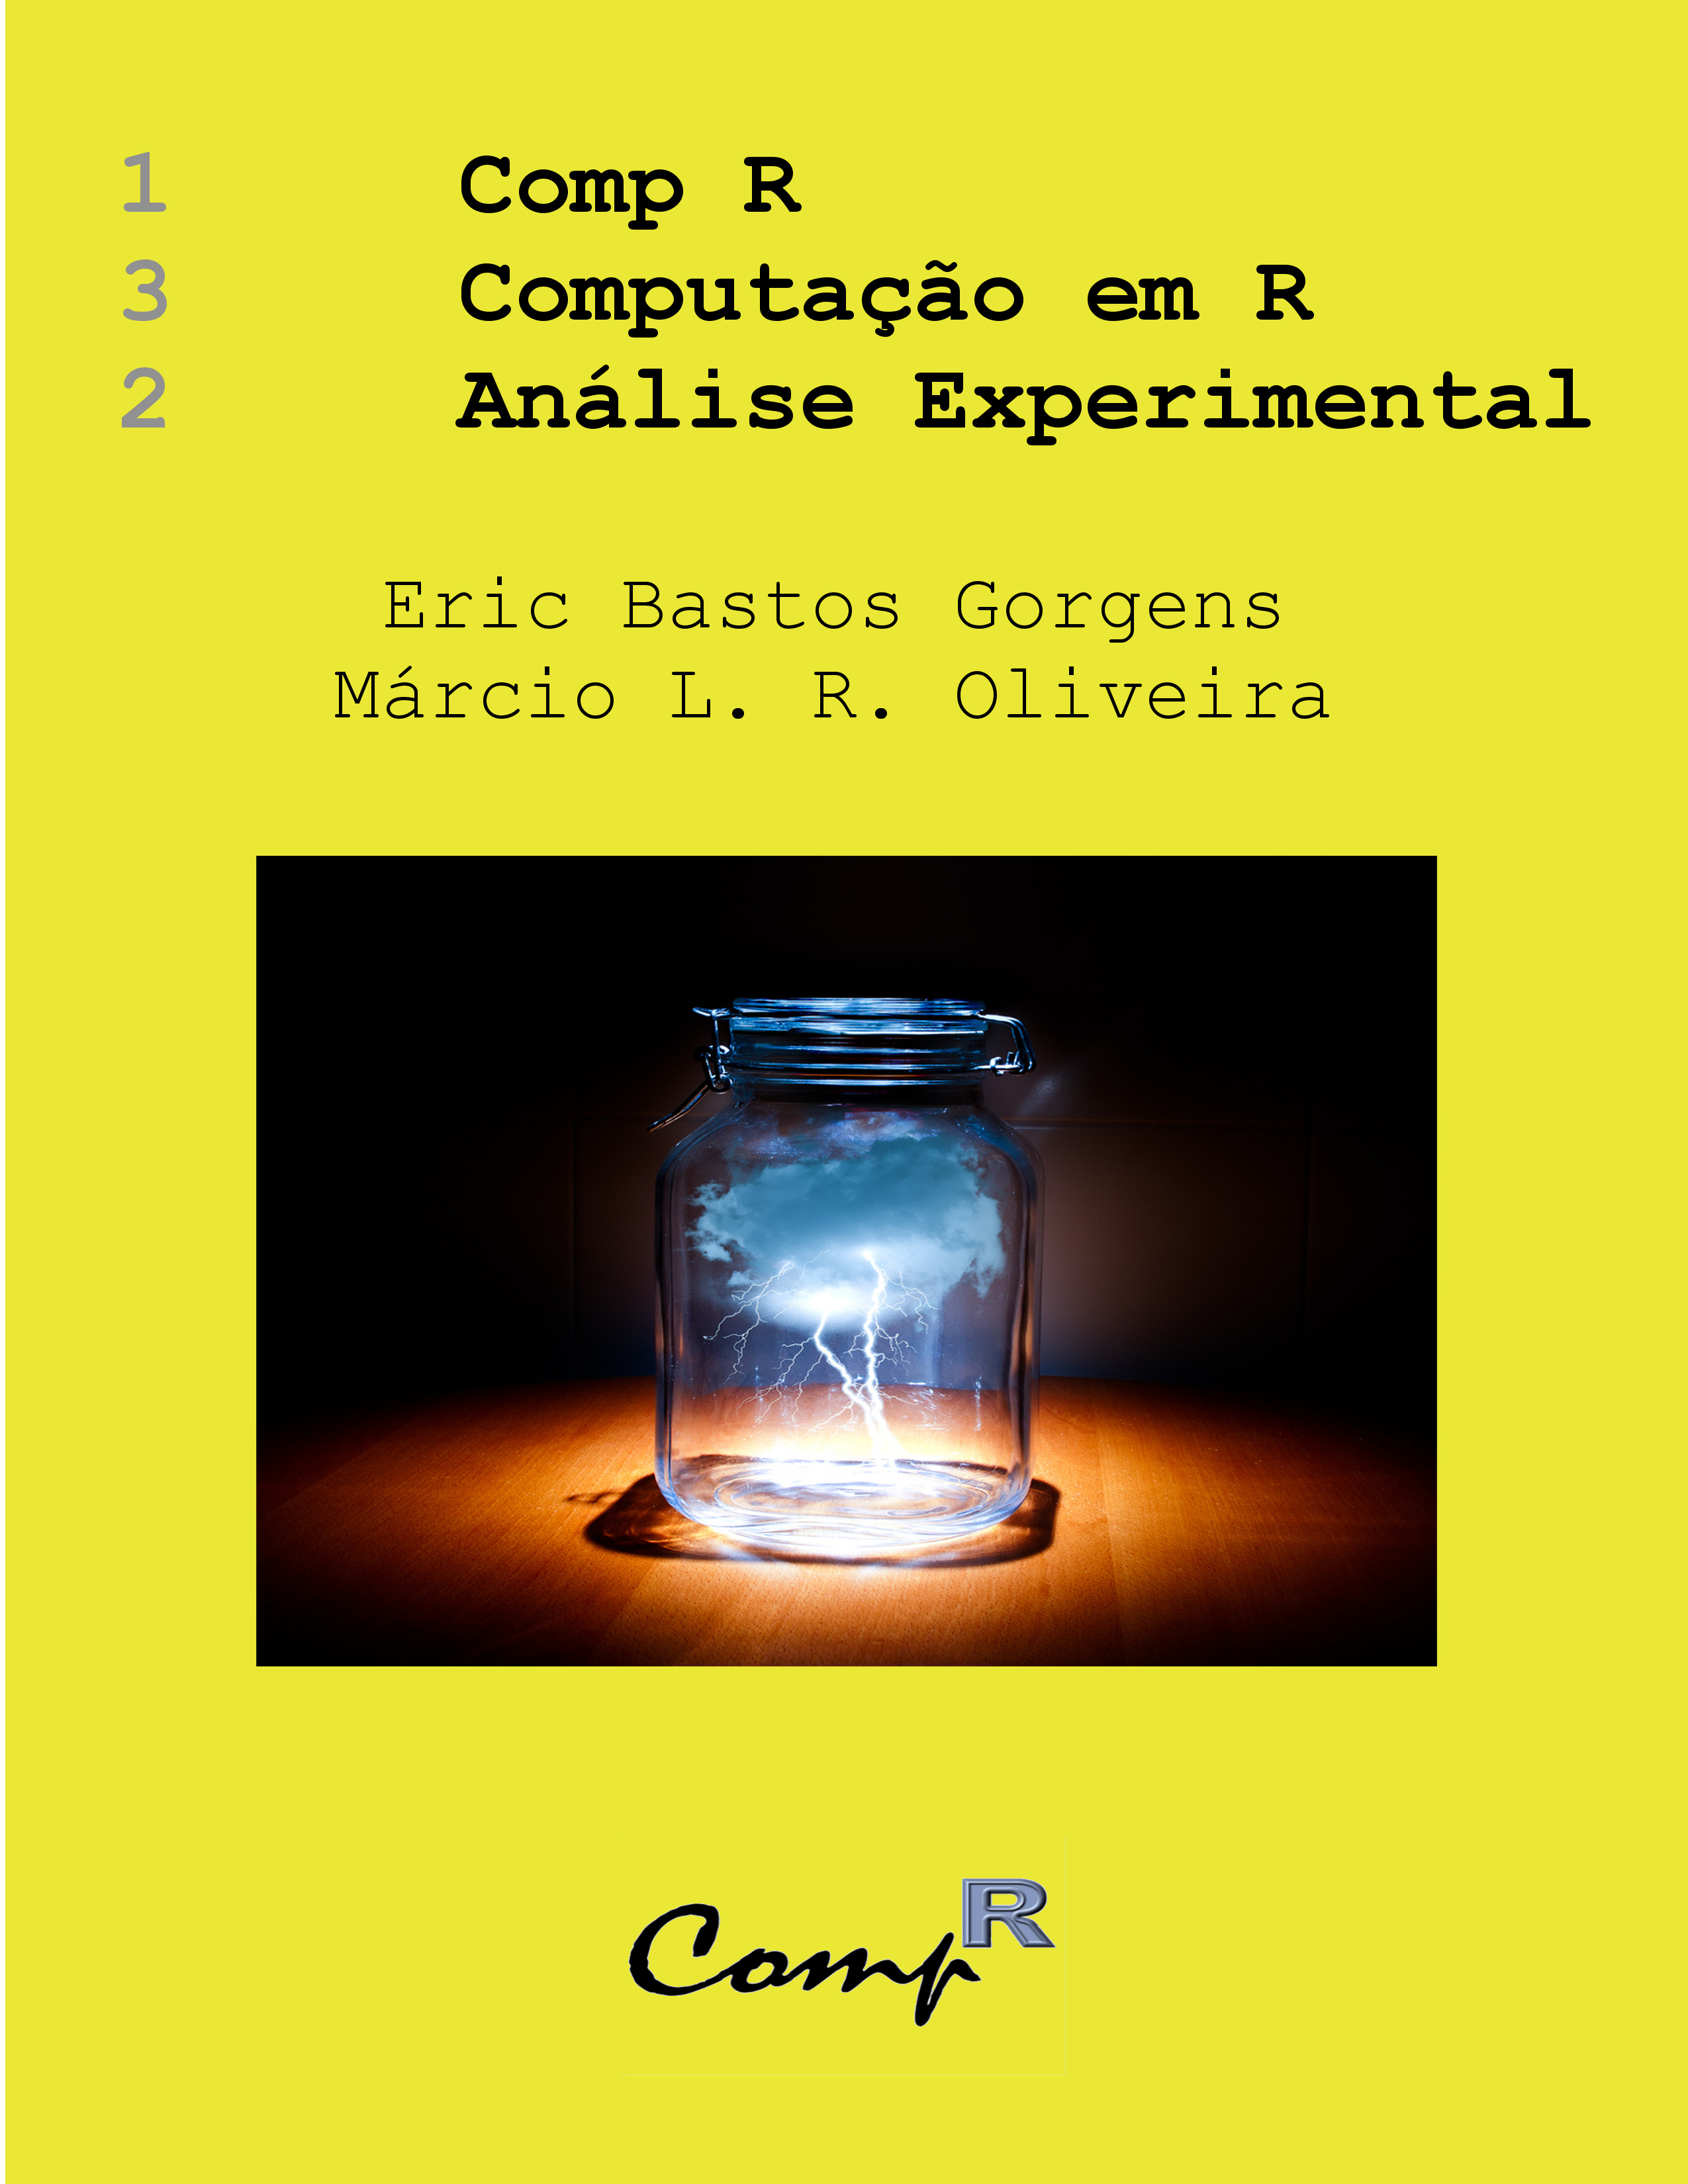
\includegraphics{./figuras/capa.png}
\caption{Capa}
\end{figure}

Bem-vindo ao mundo do R. O R não é só um software, nem se resume a uma linguagem. O R é um estilo de pesquisar, estudar e ensinar. Através de seus códigos e scripts você entrará num mundo sem limites, aberto à experimentação e à troca de experiência. Um mundo em que não existe apenas uma forma de se chegar à resposta correta, mas sim uma gama de alternativas! Você deve estar se perguntando: porque começar a trabalhar com o R? A resposta passa por algumas perspectivas interessantes.

R é gratuito. Por se tratar de um projeto de código aberto, você pode usar o R sem nenhum custo adicional: ou seja sem necessidade de pagar por inscrições, assinaturas, licenças ou limitações. Sendo o R aberto, você pode ter acesso ao código e ajustá-lo às suas necessidades (para mais detalhes veja: GNU General Public License version 2). Centenas de experts ao redor do mundo fazem exatamente isto e suas contribuições beneficiam milhares de usuários do R.

R é uma linguagem. No R, você realiza uma análise escrevendo funções e scripts; e não clicando em botões na tela. Isto pode assustar e parecer difícil, mas na verdade, a linguagem R é uma linguagem simples de aprender e muito natural para análise de dados. Aprender uma linguagem tem vários benefícios. Por se tratar de uma linguagem interativa, o R promove uma oportunidade de experimentar e explorar os dados de forma profunda e detalhada. Um script documenta passo a passo da análise, do acesso aos dados até os resultados das análises, podendo ser executados a qualquer momento, por qualquer pessoa.
Gráficos e visualização de dados. Faz parte das premissas de criações do R, a certeza de que a visualização dos dados através de gráficos é uma parte essencial de qualquer análise dos dados. Como resultado, o R oferece excelentes ferramentas para criação de gráficos, de barras até multi-painéis. Os recursos gráficos do R é influenciado pelos principais pensadores da área de visualização de dados como Bill Cleveland e Edward Tufte. Gráficos do R podem ser vistos em respeitadas publicações mundiais como The New York Times, The Economist, e o blog FlowingData.

Pacote flexível de análises estatísticas. Você irá encontrar no R um conjunto de ferramentas prontamente disponíveis, desde o acesso à vários tipos de dados, até recursos para manipulação de dados, passando pelos modelos estatísticos tradicionais e modernos. Todos os recursos estão disponíveis numa plataforma orientada a objeto que torna fácil a programação e construção de relatórios.

Acesso às poderosas e avançadas técnicas estatísticas. Os principais acadêmicos e pesquisadores do mundo utilizam o R para desenvolver as novidades nas áreas de estatística, máquinas de aprendizado e modelagem. Você pode encontrar extensões para o R contendo desenvolvimento de ponta na área econômica, genética e muitos outros campos. Atualmente são mais de 2000 pacotes que incrementam o seu R disponíveis para download.

Uma brilhante e vibrante comunidade. Com centenas de contribuidores e mais de dois milhões de usuários ao redor do mundo, se você tiver uma dúvida sobre o R, as chances de alguém já ter esbarrada com este problema é muito grande. A comunidade é gigante e participativa. A mediana de tempo que uma pergunta leva para ser respondida no StackOverflow (maior comunidade de programadores do mundo) é de 0.0147 dias, o que equivale a 21 minutos.

O R é multiplataforma rodando em Linux, Mac ou Windows. Ainda é possível configurar para rodar diretamente da nuvem. O R valoriza o que a empresa tem de mais valioso: você!

Possibilidades infinitas. Com o R você não está limitado por uma sequência pré-definida de rotinas. Você pode usar todo o portfólio de códigos e soluções disponíveis na comunidade ou mesmo criar suas próprias funções. É possível inclusive combinar o R com outros recursos como uma base de dados MySQL, ou um Apache web-server, ou ainda com o Google Maps API. Qual a sua ideia?

\hypertarget{delineamentos-experimentais}{%
\section{Delineamentos experimentais}\label{delineamentos-experimentais}}

Delineamento experimental se trata do desenho do experimento. Ou seja, ele define a organização das unidades experimentais em função da pergunta científica que se deseja responder. Com base no delineamento escolhido, regras precisam ser seguidas, especialmente relacionados à maneira que os tratamentos são distribuídos nas unidades experimentais.

A unidade experimental é o objeto que identifica um sistema de interesse de uma pesquisa e representa uma unidade da população. É sobre a unidade experimental que os tratamento serão aplicados e avaliados.

Os tratamentos são variáveis manipuladas e controladas pelo pesquisador. Desta forma, qualquer outra influência tem que ocorrer ao acaso, e por isto, as unidades experimentais devem ser o homogêneas e o tratamento deve ser a ela atribuída de forma aleatória.

Outro ponto importante num delineamento experimental, é o número de repetições. Desta forma, deve haver unidades experimentais suficientes para que os tratamentos sejam aplicados e repetidos. Quanto maior o número de repetições, menor o intervalo de confiança e, portanto, mais precisa as inferências estatísticas. Existem metodologias específicas para a determinação do número ideal de repetições, mas na prática, adotam-se trabalhos anteriores como referência, ou mesmo a disponibilidade de material acaba definindo o número de repetições.

\hypertarget{anova}{%
\subsection{ANOVA}\label{anova}}

A Análise de Variância, ou simplesmente ANOVA, é uma análise estatística para determinar a contribuição de diferentes fatores na variância total de um experimento.

O método foi desenvolvido em 1925 por Ronald Fisher para experimentos balanceados, ou seja, experimentos com o mesmo número de repetições em cada tratamento. No entanto, correções foram desenvolvidas para tratar experimentos desbalanceados, como será observado mais adiante. Assim, podemos definir Análise de Variância (ANOVA) como uma técnica que decompõe a variância total e seus graus de liberdade em partes atribuídas a fatores controlados (tratamento) e a uma outra parte associada a uma causa não controlada, também chamada de resíduo.

\hypertarget{partiuxe7uxe3o-da-variauxe7uxe3o}{%
\subsubsection{Partição da variação}\label{partiuxe7uxe3o-da-variauxe7uxe3o}}

Suponha que estamos analisando o efeito de três materiais genéticos através de um experimento inteiramente casualizado. Cada tratamento foi formado por seis repetições, e cada repetição contendo 36 plantas. Tratamentos com a mesma quantidade de repetições formam um experimento balanceado. Resumindo:

\begin{itemize}
\tightlist
\item
  Um fator com 3 tratamentos (\texttt{i} variando de 1 a 3)
\item
  6 repetições por tratamento (\texttt{j} variando de 1 a 6)
\item
  18 unidades experimentais presentes no experimento
\end{itemize}

A variável de interesse é a altura. Portanto, deseja observar se os tratamentos influenciam a altura das plantas. A média das alturas das árvores de cada uma das repetições é:

\begin{table}

\caption{\label{tab:unnamed-chunk-1}Dados de exemplo.}
\centering
\begin{tabular}[t]{l|r|r|r}
\hline
Repeticao & MatGen1 & MatGen2 & MatGen3\\
\hline
Rep 1 & 21 & 19 & 18\\
\hline
Rep 2 & 20 & 19 & 18\\
\hline
Rep 3 & 20 & 17 & 15\\
\hline
Rep 4 & 17 & 13 & 13\\
\hline
Rep 5 & 18 & 16 & 13\\
\hline
Rep 6 & 17 & 14 & 13\\
\hline
\end{tabular}
\end{table}

Para analisar o experimento, será necessario obter a média e a soma para cada tratamento:

\begin{verbatim}
## Warning in read.table(file = file, header =
## header, sep = sep, quote = quote, : incomplete
## final line found by readTableHeader on './data/
## anova_sumRep.csv'
\end{verbatim}

\begin{table}

\caption{\label{tab:unnamed-chunk-2}Média e soma de cada tratamento.}
\centering
\begin{tabular}[t]{l|l|l|l}
\hline
Estatistica & MatGen1 & MatGen2 & MatGen3\\
\hline
Soma & ? & ? & ?\\
\hline
Media & ? & ? & ?\\
\hline
\end{tabular}
\end{table}

E também a soma e média geral:

\begin{verbatim}
## Warning in read.table(file = file, header =
## header, sep = sep, quote = quote, : incomplete
## final line found by readTableHeader on './data/
## anova_sumTotal.csv'
\end{verbatim}

\begin{table}

\caption{\label{tab:unnamed-chunk-3}Média e soma total.}
\centering
\begin{tabular}[t]{l|l}
\hline
Estatistica & Valor\\
\hline
Total geral & ?\\
\hline
Media Geral & ?\\
\hline
\end{tabular}
\end{table}

Todas as somas - \texttt{sum()} e médias - \texttt{mean()} que faltam nas tabelas acimas serão computadas uma a uma por meio de linhas de comando no R. Desta forma, aproveite para relembrar um pouco da sintaxe, bem como dos operadores matemáticos:

\begin{enumerate}
\def\labelenumi{\arabic{enumi}.}
\tightlist
\item
  Entrar com os vetores correspondentes a cada tratamento com os valore de suas respectivas repetições.
\end{enumerate}

\begin{Shaded}
\begin{Highlighting}[]
\NormalTok{matGen1 =}\StringTok{ }\KeywordTok{c}\NormalTok{(}\DecValTok{21}\NormalTok{, }\DecValTok{20}\NormalTok{, }\DecValTok{20}\NormalTok{, }\DecValTok{17}\NormalTok{, }\DecValTok{18}\NormalTok{, }\DecValTok{17}\NormalTok{)}
\NormalTok{matGen2 =}\StringTok{ }\KeywordTok{c}\NormalTok{(}\DecValTok{19}\NormalTok{, }\DecValTok{19}\NormalTok{, }\DecValTok{17}\NormalTok{, }\DecValTok{13}\NormalTok{, }\DecValTok{16}\NormalTok{, }\DecValTok{14}\NormalTok{)}
\NormalTok{matGen3 =}\StringTok{ }\KeywordTok{c}\NormalTok{(}\DecValTok{18}\NormalTok{, }\DecValTok{18}\NormalTok{, }\DecValTok{15}\NormalTok{, }\DecValTok{13}\NormalTok{, }\DecValTok{13}\NormalTok{, }\DecValTok{13}\NormalTok{)}
\end{Highlighting}
\end{Shaded}

\begin{enumerate}
\def\labelenumi{\arabic{enumi}.}
\setcounter{enumi}{1}
\tightlist
\item
  Calcular a soma das repetições do tratamento 1.
\end{enumerate}

\begin{Shaded}
\begin{Highlighting}[]
\NormalTok{s1 =}\StringTok{ }\KeywordTok{sum}\NormalTok{(matGen1)}
\KeywordTok{print}\NormalTok{ (}\KeywordTok{paste}\NormalTok{(}\StringTok{"Soma MATGEN1 = "}\NormalTok{, s1, }\DataTypeTok{sep =} \StringTok{" "}\NormalTok{))}
\end{Highlighting}
\end{Shaded}

\begin{verbatim}
## [1] "Soma MATGEN1 =  113"
\end{verbatim}

\begin{enumerate}
\def\labelenumi{\arabic{enumi}.}
\setcounter{enumi}{2}
\tightlist
\item
  Calcular a média das repetições do tratamento 1.
\end{enumerate}

\begin{Shaded}
\begin{Highlighting}[]
\NormalTok{m1 =}\StringTok{ }\KeywordTok{mean}\NormalTok{(matGen1)}
\KeywordTok{print}\NormalTok{ (}\KeywordTok{paste}\NormalTok{(}\StringTok{"Media MATGEN1 = "}\NormalTok{, m1, }\DataTypeTok{sep =} \StringTok{" "}\NormalTok{))}
\end{Highlighting}
\end{Shaded}

\begin{verbatim}
## [1] "Media MATGEN1 =  18.8333333333333"
\end{verbatim}

\begin{enumerate}
\def\labelenumi{\arabic{enumi}.}
\setcounter{enumi}{3}
\tightlist
\item
  Calcular a soma das repetições do tratamento 2.
\end{enumerate}

\begin{Shaded}
\begin{Highlighting}[]
\NormalTok{s2 =}\StringTok{ }\KeywordTok{sum}\NormalTok{(matGen2)}
\KeywordTok{print}\NormalTok{ (}\KeywordTok{paste}\NormalTok{(}\StringTok{"Soma MATGEN2 = "}\NormalTok{, s2, }\DataTypeTok{sep =} \StringTok{" "}\NormalTok{))}
\end{Highlighting}
\end{Shaded}

\begin{verbatim}
## [1] "Soma MATGEN2 =  98"
\end{verbatim}

\begin{enumerate}
\def\labelenumi{\arabic{enumi}.}
\setcounter{enumi}{4}
\tightlist
\item
  Calcular a média das repetições do tratamento 2.
\end{enumerate}

\begin{Shaded}
\begin{Highlighting}[]
\NormalTok{m2 =}\StringTok{ }\KeywordTok{mean}\NormalTok{(matGen2)}
\KeywordTok{print}\NormalTok{ (}\KeywordTok{paste}\NormalTok{(}\StringTok{"Media MATGEN1 = "}\NormalTok{, m2, }\DataTypeTok{sep =} \StringTok{" "}\NormalTok{))}
\end{Highlighting}
\end{Shaded}

\begin{verbatim}
## [1] "Media MATGEN1 =  16.3333333333333"
\end{verbatim}

\begin{enumerate}
\def\labelenumi{\arabic{enumi}.}
\setcounter{enumi}{5}
\tightlist
\item
  Calcular a soma das repetições do tratamento 3.
\end{enumerate}

\begin{Shaded}
\begin{Highlighting}[]
\NormalTok{s3 =}\StringTok{ }\KeywordTok{sum}\NormalTok{(matGen3)}
\KeywordTok{print}\NormalTok{ (}\KeywordTok{paste}\NormalTok{(}\StringTok{"Soma MATGEN3 = "}\NormalTok{, s3, }\DataTypeTok{sep =} \StringTok{" "}\NormalTok{))}
\end{Highlighting}
\end{Shaded}

\begin{verbatim}
## [1] "Soma MATGEN3 =  90"
\end{verbatim}

\begin{enumerate}
\def\labelenumi{\arabic{enumi}.}
\setcounter{enumi}{6}
\tightlist
\item
  Calcular a média das repetições do tratamento 3.
\end{enumerate}

\begin{Shaded}
\begin{Highlighting}[]
\NormalTok{m3 =}\StringTok{ }\KeywordTok{mean}\NormalTok{(matGen3)}
\KeywordTok{print}\NormalTok{ (}\KeywordTok{paste}\NormalTok{(}\StringTok{"Media MATGEN3 = "}\NormalTok{, m3, }\DataTypeTok{sep =} \StringTok{" "}\NormalTok{))}
\end{Highlighting}
\end{Shaded}

\begin{verbatim}
## [1] "Media MATGEN3 =  15"
\end{verbatim}

\begin{enumerate}
\def\labelenumi{\arabic{enumi}.}
\setcounter{enumi}{7}
\tightlist
\item
  Calcular a soma de todas as repetições, dos três tratamentos.
\end{enumerate}

\begin{Shaded}
\begin{Highlighting}[]
\NormalTok{somaTotal =}\StringTok{ }\KeywordTok{sum}\NormalTok{(}\KeywordTok{c}\NormalTok{(matGen1, matGen2, matGen3))}
\KeywordTok{print}\NormalTok{ (}\KeywordTok{paste}\NormalTok{(}\StringTok{"Soma total = "}\NormalTok{, somaTotal, }\DataTypeTok{sep =} \StringTok{" "}\NormalTok{))}
\end{Highlighting}
\end{Shaded}

\begin{verbatim}
## [1] "Soma total =  301"
\end{verbatim}

\begin{enumerate}
\def\labelenumi{\arabic{enumi}.}
\setcounter{enumi}{8}
\tightlist
\item
  Calcular a média geral de todos os tratamentos e repetições.
\end{enumerate}

\begin{Shaded}
\begin{Highlighting}[]
\NormalTok{mediaGeral =}\StringTok{ }\KeywordTok{mean}\NormalTok{(}\KeywordTok{c}\NormalTok{(matGen1, matGen2, matGen3))}
\KeywordTok{print}\NormalTok{ (}\KeywordTok{paste}\NormalTok{(}\StringTok{"Media geral = "}\NormalTok{, mediaGeral, }\DataTypeTok{sep =} \StringTok{" "}\NormalTok{))}
\end{Highlighting}
\end{Shaded}

\begin{verbatim}
## [1] "Media geral =  16.7222222222222"
\end{verbatim}

A partir dos resultados obtidos nas etapas anteriores, as tabelas ficarão assim:

\begin{verbatim}
## Warning in read.table(file = file, header =
## header, sep = sep, quote = quote, : incomplete
## final line found by readTableHeader on './data/
## anova_sumRep2.csv'
\end{verbatim}

\begin{table}

\caption{\label{tab:unnamed-chunk-13}Média e soma de cada tratamento calculado.}
\centering
\begin{tabular}[t]{l|r|r|r}
\hline
Estatistica & MatGen1 & MatGen2 & MatGen3\\
\hline
Soma & 113.00 & 98.00 & 90\\
\hline
Media & 18.83 & 16.33 & 15\\
\hline
\end{tabular}
\end{table}

\begin{verbatim}
## Warning in read.table(file = file, header =
## header, sep = sep, quote = quote, : incomplete
## final line found by readTableHeader on './data/
## anova_sumTotal2.csv'
\end{verbatim}

\begin{table}

\caption{\label{tab:unnamed-chunk-14}Média e soma total calculado.}
\centering
\begin{tabular}[t]{l|r}
\hline
Estatistica & Valor\\
\hline
Total geral & 301.00\\
\hline
Media Geral & 16.72\\
\hline
\end{tabular}
\end{table}

\hypertarget{soma-de-quadrados-total}{%
\paragraph{Soma de quadrados total}\label{soma-de-quadrados-total}}

O próximo passo é analisar a diferença de cada uma das 18 observações (3 tratamentos * 6 repetições cada) em relação à média geral:

\[desvio = x_{ij} - \bar{x}\]

em que \texttt{j} indica a repetição variando de 1 a 6; e \texttt{i} indica o tratamento variando de 1 a 3.

No R, esta operação fica fácil, pois é possível fazer de uma única vez a subtração dos elementos de um vetor pela média geral:

\begin{Shaded}
\begin{Highlighting}[]
\NormalTok{desvio1 =}\StringTok{ }\NormalTok{matGen1 }\OperatorTok{-}\StringTok{ }\NormalTok{mediaGeral}
\NormalTok{desvio1}
\end{Highlighting}
\end{Shaded}

\begin{verbatim}
## [1] 4.2777778 3.2777778 3.2777778 0.2777778
## [5] 1.2777778 0.2777778
\end{verbatim}

\begin{Shaded}
\begin{Highlighting}[]
\NormalTok{desvio2 =}\StringTok{ }\NormalTok{matGen2 }\OperatorTok{-}\StringTok{ }\NormalTok{mediaGeral}
\NormalTok{desvio2}
\end{Highlighting}
\end{Shaded}

\begin{verbatim}
## [1]  2.2777778  2.2777778  0.2777778 -3.7222222
## [5] -0.7222222 -2.7222222
\end{verbatim}

\begin{Shaded}
\begin{Highlighting}[]
\NormalTok{desvio3 =}\StringTok{ }\NormalTok{matGen3 }\OperatorTok{-}\StringTok{ }\NormalTok{mediaGeral}
\NormalTok{desvio3}
\end{Highlighting}
\end{Shaded}

\begin{verbatim}
## [1]  1.277778  1.277778 -1.722222 -3.722222
## [5] -3.722222 -3.722222
\end{verbatim}

Tabulando os desvios calculados acima, tem-se uma tabela da seguinte forma:

\begin{table}

\caption{\label{tab:unnamed-chunk-16}Desvio da observação para e média geral.}
\centering
\begin{tabular}[t]{r|r|r}
\hline
MatGen1 & MatGen2 & MatGen3\\
\hline
4.28 & 2.28 & 1.28\\
\hline
3.28 & 2.28 & 1.28\\
\hline
3.28 & 0.28 & 1.72\\
\hline
0.28 & -3.72 & -3.72\\
\hline
1.28 & -0.72 & -3.72\\
\hline
0.28 & -2.72 & -3.72\\
\hline
\end{tabular}
\end{table}

Elevando cada um dos desvios ao quadrado e somando, obtem-se a soma de quadrados total (SQTotal). Esta soma de quadrados é a variação total dos dados.

\[SQTotal = \sum (x_{ij} - \bar{x})^2\]

em que \texttt{i} indica a repetição variando de 1 a 6 e \texttt{j} indica o tratamento variando de 1 a 3. A soma de quadrados total pode ser obtida com:

\begin{Shaded}
\begin{Highlighting}[]
\NormalTok{sqTotal =}\StringTok{ }\KeywordTok{sum}\NormalTok{(desvio1}\OperatorTok{^}\DecValTok{2}\NormalTok{, desvio2}\OperatorTok{^}\DecValTok{2}\NormalTok{, desvio3}\OperatorTok{^}\DecValTok{2}\NormalTok{)}
\KeywordTok{print}\NormalTok{(sqTotal)}
\end{Highlighting}
\end{Shaded}

\begin{verbatim}
## [1] 121.6111
\end{verbatim}

\hypertarget{soma-de-quadrados-dos-tratamentos}{%
\paragraph{Soma de quadrados dos tratamentos}\label{soma-de-quadrados-dos-tratamentos}}

A soma de quadrados dos tratamentos, ou a soma de quadrados entre os tratamentos, pode ser calculada pela diferença entre a média de cada tratamento em relação à média geral.

\[desvio_{i} = \bar{x}_{i} - \bar{x}\]

em que \texttt{j} indica a repetição variando de 1 a 6 e \texttt{i} indica o tratamento variando de 1 a 3. Para isto, o valor de cada repetição é substituído pela média do seu tratamento. Isto é, através da fórmula \texttt{rep}, cria-se um vetor com a média do material genético repetida 6 vezes. Com esse procedimento, elimina-se o efeito do erro, já que cada tratamento será representado \texttt{j} vezes pelo valor da sua média. Finalmente, cada repetição é subtraída pela média geral.

\begin{Shaded}
\begin{Highlighting}[]
\NormalTok{desvioTrat1 =}\StringTok{ }\KeywordTok{rep}\NormalTok{(}\KeywordTok{mean}\NormalTok{(matGen1), }\DecValTok{6}\NormalTok{) }\OperatorTok{-}\StringTok{ }\NormalTok{mediaGeral}
\NormalTok{desvioTrat1}
\end{Highlighting}
\end{Shaded}

\begin{verbatim}
## [1] 2.111111 2.111111 2.111111 2.111111 2.111111
## [6] 2.111111
\end{verbatim}

\begin{Shaded}
\begin{Highlighting}[]
\NormalTok{desvioTrat2 =}\StringTok{ }\KeywordTok{rep}\NormalTok{(}\KeywordTok{mean}\NormalTok{(matGen2), }\DecValTok{6}\NormalTok{) }\OperatorTok{-}\StringTok{ }\NormalTok{mediaGeral}
\NormalTok{desvioTrat2}
\end{Highlighting}
\end{Shaded}

\begin{verbatim}
## [1] -0.3888889 -0.3888889 -0.3888889 -0.3888889
## [5] -0.3888889 -0.3888889
\end{verbatim}

\begin{Shaded}
\begin{Highlighting}[]
\NormalTok{desvioTrat3 =}\StringTok{ }\KeywordTok{rep}\NormalTok{(}\KeywordTok{mean}\NormalTok{(matGen3), }\DecValTok{6}\NormalTok{) }\OperatorTok{-}\StringTok{ }\NormalTok{mediaGeral}
\NormalTok{desvioTrat3}
\end{Highlighting}
\end{Shaded}

\begin{verbatim}
## [1] -1.722222 -1.722222 -1.722222 -1.722222
## [5] -1.722222 -1.722222
\end{verbatim}

Trazendo os resultados do R para uma tabela de desvios tem-se:

\begin{table}

\caption{\label{tab:unnamed-chunk-19}Desvio entre a média do tratamento e média geral.}
\centering
\begin{tabular}[t]{r|r|r}
\hline
MatGen1 & MatGen2 & MatGen3\\
\hline
2.11 & -0.39 & -1.72\\
\hline
2.11 & -0.39 & -1.72\\
\hline
2.11 & -0.39 & -1.72\\
\hline
2.11 & -0.39 & -1.72\\
\hline
2.11 & -0.39 & -1.72\\
\hline
2.11 & -0.39 & -1.72\\
\hline
\end{tabular}
\end{table}

Os desvios são então elevados ao quadrado e somados, resultando na soma de quadrados dos tratamentos (SQTrat):

\begin{Shaded}
\begin{Highlighting}[]
\NormalTok{sqTrat =}\StringTok{ }\KeywordTok{sum}\NormalTok{(desvioTrat1}\OperatorTok{^}\DecValTok{2}\NormalTok{, desvioTrat2}\OperatorTok{^}\DecValTok{2}\NormalTok{, desvioTrat3}\OperatorTok{^}\DecValTok{2}\NormalTok{)}
\KeywordTok{print}\NormalTok{(sqTrat)}
\end{Highlighting}
\end{Shaded}

\begin{verbatim}
## [1] 45.44444
\end{verbatim}

\hypertarget{soma-de-quadrados-dos-resuxedduos}{%
\paragraph{Soma de quadrados dos resíduos}\label{soma-de-quadrados-dos-resuxedduos}}

A soma de quadrados dos resíduos (SQRes) é também conhecida como soma de quadrados dentro do tratamento. Primeiro, calcula-se o desvio entre a cada uma das repetições e a média do respectivo tratamento:

\[desvio = x_{ij} - \bar{x}_{i}\]
No R, podemos calcular da seguinte forma:

\begin{Shaded}
\begin{Highlighting}[]
\NormalTok{desvioRes1 =}\StringTok{ }\NormalTok{matGen1 }\OperatorTok{-}\StringTok{ }\KeywordTok{mean}\NormalTok{(matGen1)}
\NormalTok{desvioRes1}
\end{Highlighting}
\end{Shaded}

\begin{verbatim}
## [1]  2.1666667  1.1666667  1.1666667 -1.8333333
## [5] -0.8333333 -1.8333333
\end{verbatim}

\begin{Shaded}
\begin{Highlighting}[]
\NormalTok{desvioRes2 =}\StringTok{ }\NormalTok{matGen2 }\OperatorTok{-}\StringTok{ }\KeywordTok{mean}\NormalTok{(matGen2)}
\NormalTok{desvioRes2}
\end{Highlighting}
\end{Shaded}

\begin{verbatim}
## [1]  2.6666667  2.6666667  0.6666667 -3.3333333
## [5] -0.3333333 -2.3333333
\end{verbatim}

\begin{Shaded}
\begin{Highlighting}[]
\NormalTok{desvioRes3 =}\StringTok{ }\NormalTok{matGen3 }\OperatorTok{-}\StringTok{ }\KeywordTok{mean}\NormalTok{(matGen3)}
\NormalTok{desvioRes3}
\end{Highlighting}
\end{Shaded}

\begin{verbatim}
## [1]  3  3  0 -2 -2 -2
\end{verbatim}

Trazendo os resultados do R para uma tabela de desvios tem-se:

\begin{table}

\caption{\label{tab:unnamed-chunk-22}Desvio da observação para e média do tratamento}
\centering
\begin{tabular}[t]{r|r|r}
\hline
MatGen1 & MatGen2 & MatGen3\\
\hline
2.17 & 2.67 & 3\\
\hline
1.17 & 2.67 & 3\\
\hline
1.17 & 0.67 & 0\\
\hline
-1.83 & -3.33 & -2\\
\hline
0.83 & 0.33 & -2\\
\hline
-1.83 & -2.33 & -2\\
\hline
\end{tabular}
\end{table}

Elevando cada desvio ao quadrado e somando-os, calcula-se a soma de quadrados dos resíduos:

\begin{Shaded}
\begin{Highlighting}[]
\NormalTok{sqRes =}\StringTok{ }\KeywordTok{sum}\NormalTok{(desvioRes1}\OperatorTok{^}\DecValTok{2}\NormalTok{, desvioRes2}\OperatorTok{^}\DecValTok{2}\NormalTok{, desvioRes3}\OperatorTok{^}\DecValTok{2}\NormalTok{)}
\KeywordTok{print}\NormalTok{(sqRes)}
\end{Highlighting}
\end{Shaded}

\begin{verbatim}
## [1] 76.16667
\end{verbatim}

\hypertarget{quadrado-muxe9dio}{%
\paragraph{Quadrado médio}\label{quadrado-muxe9dio}}

O próximo passo é montar o quadro da ANOVA e determinar os quadrados médios:

\begin{verbatim}
## Warning in read.table(file = file, header = header,
## sep = sep, quote = quote, : incomplete final line
## found by readTableHeader on './data/anova_qm.csv'
\end{verbatim}

\begin{table}

\caption{\label{tab:unnamed-chunk-24}Fórmulas para o caluclo do quandrado médio.}
\centering
\begin{tabular}[t]{l|l|l|l}
\hline
Fonte.de.variacao & Soma.de.quadrados & Graus.de.liberdade & Quadrado.medio\\
\hline
Trat & SQTrat & \$i-1\$ & \$SQTotal / (i-1)\$\\
\hline
Residuos & SQRes & \$i * (j - 1)\$ & \$SQRes / (i * (j-1))\$\\
\hline
Total & SQTotal & \$(i * j) - 1\$ & \\
\hline
\end{tabular}
\end{table}

Tanto a soma de quadrados, como os graus de liberdade são aditivos. Isto é, obtendo dois termos do quadro de variância, o terceiro pode ser obtido pela diferença.

Na prática, calcula-se a soma de quadrados total e a soma de quadrados do tratamento. Por diferença, obtém-se a soma de quadrados dos resíduos. O mesmo raciocínio vale para os graus de liberdade.

O quadrado médio, nada mais é que uma variância. Por isso, divide-se a soma de quadrados pelos graus de liberdade. Os quadrados médios são calculados da seguinte forma:

\begin{enumerate}
\def\labelenumi{\arabic{enumi}.}
\tightlist
\item
  Quadrado médio dos tratamentos
\end{enumerate}

\begin{Shaded}
\begin{Highlighting}[]
\NormalTok{qmTrat =}\StringTok{ }\NormalTok{sqTrat }\OperatorTok{/}\StringTok{ }\NormalTok{(}\DecValTok{3} \OperatorTok{-}\StringTok{ }\DecValTok{1}\NormalTok{)}
\KeywordTok{print}\NormalTok{(qmTrat)}
\end{Highlighting}
\end{Shaded}

\begin{verbatim}
## [1] 22.72222
\end{verbatim}

\begin{enumerate}
\def\labelenumi{\arabic{enumi}.}
\setcounter{enumi}{1}
\tightlist
\item
  Quadrado médio do residuo
\end{enumerate}

\begin{Shaded}
\begin{Highlighting}[]
\NormalTok{qmRes =}\StringTok{ }\NormalTok{sqRes }\OperatorTok{/}\StringTok{ }\NormalTok{(}\DecValTok{3} \OperatorTok{*}\StringTok{ }\NormalTok{(}\DecValTok{6} \OperatorTok{-}\StringTok{ }\DecValTok{1}\NormalTok{))}
\KeywordTok{print}\NormalTok{(qmRes)}
\end{Highlighting}
\end{Shaded}

\begin{verbatim}
## [1] 5.077778
\end{verbatim}

\hypertarget{teste-f}{%
\paragraph{Teste F}\label{teste-f}}

Assim, o objetivo final da ANOVA é comparar a variância dos tratamentos relativa à variância dos resíduos. O valor da razão entre estas duas variâncias segue a distribuição F, recorrendo-se então à uma tabela de distribuição amostral da razão F para avaliar a significância do teste.

\begin{Shaded}
\begin{Highlighting}[]
\NormalTok{Fcalc =}\StringTok{ }\NormalTok{qmTrat }\OperatorTok{/}\StringTok{ }\NormalTok{qmRes}
\KeywordTok{print}\NormalTok{(Fcalc)}
\end{Highlighting}
\end{Shaded}

\begin{verbatim}
## [1] 4.474836
\end{verbatim}

O quadro final da ANOVA será:

\begin{verbatim}
## Warning in read.table(file = file, header =
## header, sep = sep, quote = quote, : incomplete
## final line found by readTableHeader on './data/
## anova_final.csv'
\end{verbatim}

\begin{table}

\caption{\label{tab:unnamed-chunk-28}Quandro final da ANOVA}
\centering
\begin{tabular}[t]{l|r|r|r|r}
\hline
Fonte.de.variacao & Soma.de.quadrados & Graus.de.liberdade & Quadrado.medio & FCalc\\
\hline
Trat & 45.44 & 2 & 22.72 & 4.47\\
\hline
Resíduos & 76.17 & 15 & 5.08 & NA\\
\hline
Total & 121.61 & 17 & NA & NA\\
\hline
\end{tabular}
\end{table}

A hipótese nula é de que a variância entre os tratamentos é igual à variância populacional, ou variância dos resíduos. Um teste não significativo aceita-se a hipótese nula. Já um teste significativo rejeita-se a hipótese nula.

\begin{Shaded}
\begin{Highlighting}[]
\NormalTok{Ftabelado =}\StringTok{ }\KeywordTok{qf}\NormalTok{(}\FloatTok{0.95}\NormalTok{, }\DecValTok{2}\NormalTok{, }\DecValTok{15}\NormalTok{)}
\KeywordTok{print}\NormalTok{(Ftabelado)}
\end{Highlighting}
\end{Shaded}

\begin{verbatim}
## [1] 3.68232
\end{verbatim}

Neste exercício, o \texttt{F} calculado é superior ao \texttt{F} tabelado. Assim o teste F é significativo e a hipótese nula é rejeitada para um nível de significância de 95\%. A variância dos tratamentos não pode ser considerada igual à variância da população. Na prática isto indica que existe um efeito significativo dos tratamentos, e que pelo menor um dos tratamentos diferem dos demais.

Se o teste F é não significativo (\texttt{F\ calculado\ \textless{}\ F\ tabelado}), entende-se que os tratamentos não influenciaram as observações e a análise de seu experimento encerra-se aqui.

Por outro lado, o teste F significativo indica que pelo menos um dos tratamentos influenciou os dados observados. Se apenas dois tratamentos tiverem sido realizados, o teste F é conclusivo e as médias dos tratamentos podem ser comparadas diretamente. Se três ou mais tratamentos estiverem sendo comparados, o teste F é inconclusivo, uma vez que diz apenas que existe uma influência dos tratamentos, sem no entanto indicar qual deles é igual ou diferente. Assim uma pergunta surge: como os tratamentos se diferem uns dos outros?

Entram em cena os testes de médias ou a análise de regressão. Quando os tratamentos são qualitativos e significativos, o teste de médias irá dizer quais tratamentos são iguais e quais tratamentos são diferentes. Quando os tratamentos são quantitativos e significativos, utiliza-se a análise de regressão para definir o ponto ótimo. Dependendo do objetivo do experimento, mesmo tratamentos quantitativos podem ser analisados por meio de um teste de médias.

Para facilitar, a figura a seguir resume o que foi visto até agora por meio de uma árvore de decisão:

\begin{figure}
\centering
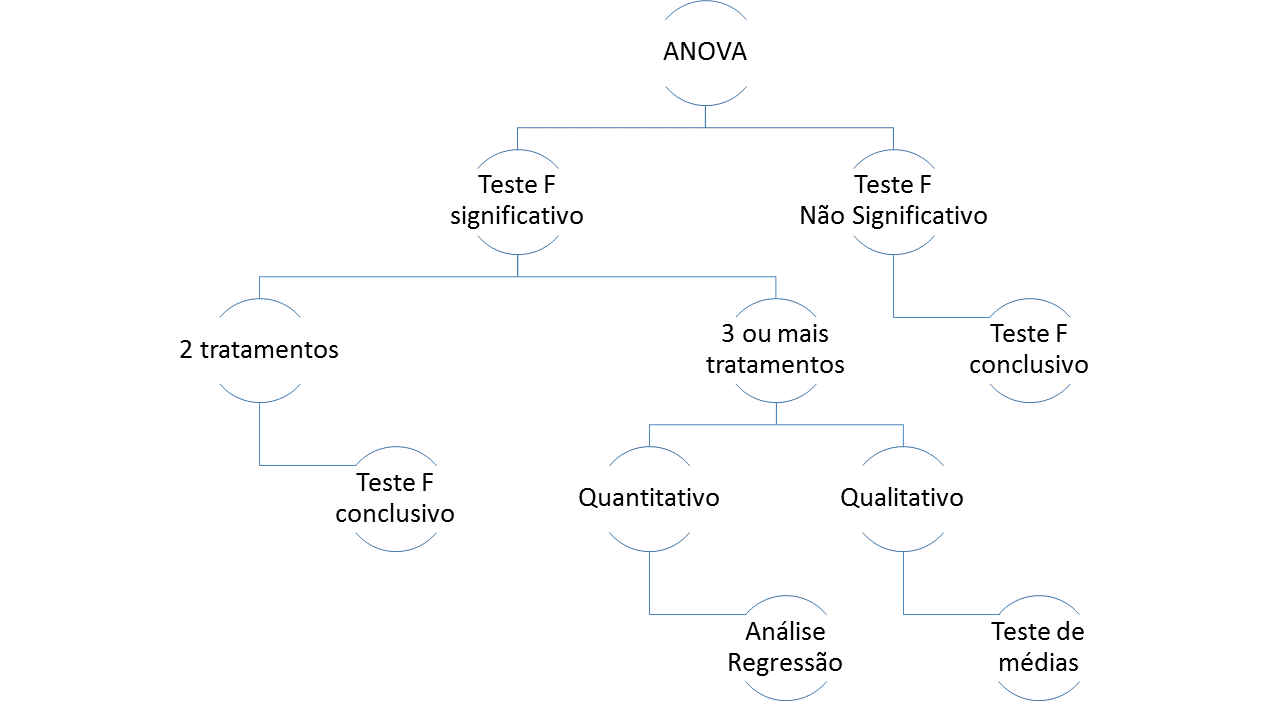
\includegraphics{./figuras/resumo_anova.png}
\caption{Fluxograma de decisão para interpretação de uma ANOVA}
\end{figure}

\hypertarget{tipos-de-anova}{%
\subsection{Tipos de ANOVA}\label{tipos-de-anova}}

Existem pelo menos 3 formas para se calcular a soma de quadrados da ANOVA, que são conhecidos como soma de quadrados do TIPO I, TIPO II e TIPO III. Esta notação foi introduzida pelo software SAS, mas acabou sendo adotada pela comunidade para diferenciar entre as diferentes formas de se calcular a soma de quadrados para composição da ANOVA.

A recomendação de uso dos diferentes tipos de soma de quadrados leva a calorosas discussões entre estatísticos. De modo geral, o tipo I é o padrão usado para dados balanceados. O tipo II e tipo III são mais indicados para dados desbalanceados. Quando o experimento é balanceado, os três tipos de ANOVA apresentam resultados idênticos.

\hypertarget{variauxe7uxf5es-no-cuxe1lculo-da-soma-de-quadrados}{%
\subsubsection{Variações no cálculo da soma de quadrados}\label{variauxe7uxf5es-no-cuxe1lculo-da-soma-de-quadrados}}

Partindo de um experimento que considere dois fatores A e B; sendo dois fatores principais e a interação AB, o modelo completo pode ser representado por \texttt{SQ(A,\ B,\ AB)}. Também podem ser considerados modelos parciais como \texttt{SQ(A,\ B)} que indica um modelo sem interação, ou como \texttt{SQ(B,\ AB)} que indica um modelo que não considera efeitos do fator A.

A influência de um determinado fator (ou interação) é testada examinando as diferenças entre os modelos. Por exemplo, para determinar a presença de interação entre os fatores, um teste F é conduzido comparando o modelo com interação \texttt{SQ(A,\ B,\ AB)} e o modelo sem interação \texttt{SQ(A,\ B)}.

\hypertarget{anova-tipo-i}{%
\subsubsection{ANOVA Tipo I}\label{anova-tipo-i}}

A ANOVA tipo I testa primeiro o efeito de A, seguido do efeito de B dado que se conhece A, seguido pela interação dado que os efeitos principais já são conhecidos. Esta ordem natural (\texttt{A\ -\textgreater{}\ B\ -\textgreater{}\ AB}) é a razão desta ANOVA ser conhecida como soma de quadrados sequencial.

\begin{enumerate}
\def\labelenumi{\arabic{enumi}.}
\tightlist
\item
  \texttt{SQ(A)} para o fator A.
\item
  \texttt{SQ(B\ \textbar{}\ A)} para fator B.
\item
  \texttt{SQ(AB\ \textbar{}\ B,\ A)} para interação AB.
\end{enumerate}

\hypertarget{anova-tipo-ii}{%
\subsubsection{ANOVA Tipo II}\label{anova-tipo-ii}}

Este tipo de ANOVA testa o efeito de um dos fatores principais dado que o outro já é conhecido. Assim, assume-se a não significância da interação.

Sugere-se no entanto que se teste \texttt{SQ(AB\ \textbar{}\ A,\ B)}. Se de fato a interação for não significativa, então o tipo II é estatisticamente mais poderoso que o tipo III.

\begin{enumerate}
\def\labelenumi{\arabic{enumi}.}
\tightlist
\item
  \texttt{SQ(A\ \textbar{}\ B)} para o fator A.
\item
  \texttt{SQ(B\ \textbar{}\ A)} para o fator B.
\end{enumerate}

\hypertarget{anova-tipo-iii}{%
\subsubsection{ANOVA Tipo III}\label{anova-tipo-iii}}

Este tipo de ANOVA só é válido quando a interação é significativa. No entanto, em muitos casos não se tem interesse em analisar os fatores principais quando a interação está presente, ou seja, na presença de interação, os efeitos principais deixam de ser interessantes isoladamente.

\begin{enumerate}
\def\labelenumi{\arabic{enumi}.}
\tightlist
\item
  \texttt{SQ(A\ \textbar{}\ B,\ AB)} para o fator A.
\item
  \texttt{SQ(B\ \textbar{}\ A,\ AB)} para o fator B.
\end{enumerate}

Assim, na prática, só é necessário preocupar com dados desbalanceados quando a interação entre fontes de variação for considerada no modelo estatístico do experimento.

\hypertarget{pressuposiuxe7uxf5es-e-transformauxe7uxf5es}{%
\section{Pressuposições e transformações}\label{pressuposiuxe7uxf5es-e-transformauxe7uxf5es}}

Duas são as pressuposições da ANOVA:

\begin{itemize}
\tightlist
\item
  Homogeneidade de variâncias
\item
  Normalidade dos resíduos
\end{itemize}

Neste momento, não se preocupe com os testes estatísticos utilizados para a verificação dessas pressuposições. Até mesmo, porque as pressuposições precisam ser analisadas após a análise de variância ser realizada, já que a normalidade da variável não garante a normalidade dos resíduos.

No caso de uma das pressuposições não serem atendidas, os dados devem ser transformados, a análise refeita e as pressuposições novamente verificadas. Na sequência serao apresentadas as principais transformações usadas na área das ciências florestais e biológicas.

\hypertarget{transformauxe7uxe3o-logaruxedtmica}{%
\subsection{Transformação Logarítmica}\label{transformauxe7uxe3o-logaruxedtmica}}

Esta transformação é indicada para variáveis contínuas e consiste em obter o \texttt{log} de cada uma das observações. É possível usar tanto o log base 10 quanto o log base \textbf{e}. Utilizar um ou outro não faz nenhuma diferença para o teste estatístico, pois a única diferença é a constante logarítmica.

Não deixe de registrar qual a base foi utilizada já que esta decisão influencia a interpretação do coeficiente angular e o coeficiente de inclinação da regressão num eventual desdobramento.

\begin{Shaded}
\begin{Highlighting}[]
\NormalTok{a =}\StringTok{ }\FloatTok{5.7}
\NormalTok{trans_a =}\StringTok{ }\KeywordTok{log}\NormalTok{(a)}
\end{Highlighting}
\end{Shaded}

Para reverter a transformação logarítmica:

\begin{Shaded}
\begin{Highlighting}[]
\KeywordTok{exp}\NormalTok{(trans_a)}
\end{Highlighting}
\end{Shaded}

\begin{verbatim}
## [1] 5.7
\end{verbatim}

Lembre-se de que se os dados possuem zeros ou valores negativos, não se pode usar a transformação logarítmica. Uma saída é adicionar uma constante a cada número para torná-lo positivo e não zero. Se os dados forem contagem com presença de zero, a solução é adicionar 0,5 a cada observação.

Muitas variáveis biológicas tem distribuição log-normal. Desta forma, após a transformação logarítmica, os valores passam a ter distribuição normal. O produto de conjunto de fatores independentes é log-normal. Por exemplo, a altura de uma árvore é uma função de (nitrogênio x água x luz x pragas). Matematicamente esta função é uma log-normal.

\hypertarget{transformauxe7uxe3o-da-raiz-quadrada}{%
\subsection{Transformação da Raiz quadrada}\label{transformauxe7uxe3o-da-raiz-quadrada}}

Esta transformação consiste na obtenção da raiz quadrada de cada uma das observações. Esta transformação é muito utilizada para variáveis de contagem. No entanto ela só pode ser utilizada para dados positivos. Em caso de número negativos, uma saída é adicionar uma constante a todas as observações eliminando assim as observações negativas.

\begin{Shaded}
\begin{Highlighting}[]
\NormalTok{b =}\StringTok{ }\DecValTok{10}
\NormalTok{trans_b =}\StringTok{ }\KeywordTok{sqrt}\NormalTok{(b)}
\end{Highlighting}
\end{Shaded}

Para reverter a transformação:

\begin{Shaded}
\begin{Highlighting}[]
\NormalTok{trans_b}\OperatorTok{^}\DecValTok{2}
\end{Highlighting}
\end{Shaded}

\begin{verbatim}
## [1] 10
\end{verbatim}

\hypertarget{transformauxe7uxe3o-do-arcoseno}{%
\subsection{Transformação do Arcoseno}\label{transformauxe7uxe3o-do-arcoseno}}

Esta transformação consiste em calcular o arcoseno da raiz quadrada de cada uma das observações. O resultado é dado em radianos e não em graus, e pode variar de -π/2 a π/2. Os números para serem transformados pelo arcoseno precisam estar entre -1 e 1. Por isso, é comum utilizar esta transformação para proporções, cuja amplitude geralmente está entre 0 e 1

\begin{Shaded}
\begin{Highlighting}[]
\NormalTok{c =}\StringTok{ }\FloatTok{0.8}
\NormalTok{trans_c =}\StringTok{ }\KeywordTok{asin}\NormalTok{(}\KeywordTok{sqrt}\NormalTok{(c))}
\end{Highlighting}
\end{Shaded}

Para reverter a transformação:

\begin{Shaded}
\begin{Highlighting}[]
\NormalTok{(}\KeywordTok{sin}\NormalTok{(trans_c))}\OperatorTok{^}\DecValTok{2}
\end{Highlighting}
\end{Shaded}

\begin{verbatim}
## [1] 0.8
\end{verbatim}

\hypertarget{anova-no-r}{%
\section{ANOVA no R}\label{anova-no-r}}

Este capítulo começa com uma boa notícia. O R conta com diversos pacotes desenvolvidos que realizam toda a sequência de uma análise de variância, tanto para o caso balanceado, quanto para o caso desbalanceado. Ao longo deste livro serão utilizados dois pacotes:

\begin{itemize}
\tightlist
\item
  \texttt{ExpDes.pt}
\item
  \texttt{easyanova}
\end{itemize}

Os pacotes no R são desenvolvidos e disponibilizados de forma oficial no repositório chamado de CRAN. Embora um pacote precise seguir determinadas regras mínimas para ser disponibilizado no repositório oficial, o estilo de cada desenvolvedor leva a diferenças significativas nas características e no funcionamento dos pacotes.

\hypertarget{pacote-expdes.pt}{%
\subsection{Pacote ExpDes.pt}\label{pacote-expdes.pt}}

O pacote \texttt{ExpDes.pt} (e sua versão em inglês \texttt{ExpDes}) foi desenvolvido por uma equipe da Universidade de Alfenas (Unifal) composta por Eric Batista Ferreira, Pórtya Piscitelli Cavalcanti, Denismar Alves Nogueira e outros. Este pacote realiza a análise de diversos delineamentos experimentais e desdobramentos tanto de fatores qualitativos quanto de fatores quantitativos. Para instalar o \texttt{ExpDes.pt}:

\begin{Shaded}
\begin{Highlighting}[]
\KeywordTok{install.packages}\NormalTok{(}\StringTok{"ExpDes.pt"}\NormalTok{)}
\end{Highlighting}
\end{Shaded}

O pacote \texttt{ExpDes.pt} ao ser instalado trás diversas funções para analisar os seguintes delineamentos experimentais:

\begin{itemize}
\tightlist
\item
  DIC: delineamento inteiramente casualizado
\item
  DBC: delineamento em blocos casualizados
\item
  DQL: delineamento em quadrado latino
\item
  Experimentos em esquema de fatorial duplo (em DIC e DBC)
\item
  Experimentos em esquema de parcelas subdivididas (em DIC e DBC)
\item
  Experimentos em esquema de fatorial duplo com um tratamento adicional (em DIC e DBC)
\item
  Experimentos em esquema de fatorial triplo (em DIC e DBC)
\item
  Experimentos em esquema de fatorial triplo com um tratamento adicional (em DIC e DBC)
\end{itemize}

O pacote permite ainda o desdobramento de níveis quantitativos a partir de modelos de regressão até o terceiro grau. No caso de níveis qualitativos, o desdobramento ocorre por testes de comparação múltipla incluindo:

\begin{itemize}
\tightlist
\item
  Teste de Tukey
\item
  Teste de Student-Newman-Keuls (SNK)
\item
  Teste de Scott-Knott
\item
  Teste de Duncan
\item
  Teste t (LSD)
\item
  Teste t de Bonferroni (LSD protegido)
\item
  Teste Bootstrap
\end{itemize}

Mesmo depois de instalados, os pacotes precisam ser ativados antes de serem utilizados. A ativação pode ser feita pelo comando:

\begin{Shaded}
\begin{Highlighting}[]
\KeywordTok{require}\NormalTok{(ExpDes.pt)}
\end{Highlighting}
\end{Shaded}

Uma vez ativado, as funções do pacote passam a estar disponíveis para o usuário. Para conhecer os parâmetros e o funcionamento da função, a página de ajuda pode ser consultada digitando no console \texttt{?} seguido do nome da função:

\begin{Shaded}
\begin{Highlighting}[]
\NormalTok{?dic}
\end{Highlighting}
\end{Shaded}

Toda função no R é composta por parâmetros obrigatórios e parâmetros opcionais. Esta indicação será obtida analisando a sintaxe da função, também disponível na página de ajuda. Como exemplo, consultando a página de ajuda da função \texttt{dic}, nota-se que a sintaxe básica da funçao é:

\begin{Shaded}
\begin{Highlighting}[]
\KeywordTok{dic}\NormalTok{(trat, resp, }\DataTypeTok{quali =} \OtherTok{TRUE}\NormalTok{, }\DataTypeTok{mcomp =} \StringTok{"tukey"}\NormalTok{, }\DataTypeTok{sigT =} \FloatTok{0.05}\NormalTok{, }\DataTypeTok{sigF =} \FloatTok{0.05}\NormalTok{)}
\end{Highlighting}
\end{Shaded}

Pela sintaxe apresentada acima, dois parâmetros são obrigatórios: \texttt{trat} e \texttt{resp}. Estes parâmetros correspondem às colunas da nossa base de dados em que \texttt{trat} indica tratamento e \texttt{resp} indica variável resposta. Os demais parâmetros não são obrigatórios pois já estão pré-definidos. Por exemplo, o parâmetro \texttt{quali} está pré-definido como \texttt{TRUE}. Isto implica que os níveis do tratamento serão interpretados como qualitativos. Assim, se o experimento possuir tratamento com níveis quantitativos, como por exemplo dosagem de nutrientes, o parâmetro \texttt{quali} deverá ser definido como \texttt{FALSE}. Os demais parâmetros optativos indicam:

\begin{itemize}
\tightlist
\item
  \texttt{mcomp}: o teste de média que será aplicado caso seja necessário realizar o desdobramento dos tratamentos. O parâmetro vem pré-definido como Teste de Tukey (\texttt{tukey}).
\item
  \texttt{sigT}: o nível de significância para o teste de médias. Pré-definido como 5\% (\texttt{0,05}).
\item
  \texttt{sigF}: o nível de significância para o teste F da análise de variância. Pré-definido como 5\% (\texttt{0,05}).
\end{itemize}

O pacote \texttt{ExpDes.pt} só é capaz de computar a ANOVA do Tipo I, e é por isto que os experimentos desbalanceados que possuam interação não serão analisados por meio desse pacote.

\hypertarget{pacote-easyanova}{%
\subsection{Pacote easyanova}\label{pacote-easyanova}}

O pacote \texttt{easyanova} foi desenvolvido pelo professor Emmanuel Arnhold, que leciona disciplinas de estatística aplicada à experimentação agropecuária em nível de graduação e pós-graduação na Universidade Federal de Goiás (UFG). O pacote \texttt{easyanova} pode ser utilizado para qualquer tipo de experimento - balanceado e desbalanceado - já que possui um mecanismo que define o tipo de ANOVA com base na estrutura dos dados apresentados. Para instalar o \texttt{easyanova}:

\begin{Shaded}
\begin{Highlighting}[]
\KeywordTok{install.packages}\NormalTok{(}\StringTok{"easyanova"}\NormalTok{)}
\end{Highlighting}
\end{Shaded}

Estando o pacote instalado, a sua ativação pode ser feita através da função \texttt{require()}:

\begin{Shaded}
\begin{Highlighting}[]
\KeywordTok{require}\NormalTok{(easyanova)}
\end{Highlighting}
\end{Shaded}

Diferentemente do pacote \texttt{ExpDes.pt}, o easyanova possui apenas duas funções básicas para análise de experimentos:

\begin{itemize}
\tightlist
\item
  \texttt{ea1()}
\item
  \texttt{ea2()}
\end{itemize}

A definição do delineamento e/ou do esquema é feito através de um parâmetro dentro destas duas funções. Assim, através da definição do parâmetro \texttt{design}, a função \texttt{ea1()} é capaz de analisar os seguintes delineamentos:

\begin{enumerate}
\def\labelenumi{\arabic{enumi}.}
\tightlist
\item
  inteiramente casualizado
\item
  blocos casualizados
\item
  quadrado latino
\item
  several latin squares
\item
  análise de covariância (dic)
\item
  análise de covariância (dbc)
\item
  blocos incompletos tipo I e II
\item
  blocos incompletos tipo III ou blocos aumentados
\item
  blocos incompletos tipo III em experimentos com animais
\item
  lattice (intra-blocos)
\item
  lattice (inter-blocos)
\item
  switchback
\item
  switchback em blocos
\item
  teste Kruskal-Wallis
\item
  teste Friedman
\end{enumerate}

Já a função \texttt{ea2()} é capaz, através da definição do parâmetro \texttt{design}, de analisar os seguintes delineamentos:

\begin{enumerate}
\def\labelenumi{\arabic{enumi}.}
\tightlist
\item
  fatorial duplo inteiramente casualizado
\item
  fatorial duplo em blocos casualizados
\item
  fatorial duplo em quadrados latinos
\item
  parcela subdividida inteiramente casualizado
\item
  parcela subdividida em blocos casualizados
\item
  parcela dividida em quadrados latinos
\item
  fatorial triplo inteiramente casualizado
\item
  fatorial triplo em blocos casualizados
\item
  fatorial duplo em parcela subdividida (DIC)
\item
  fatorial duplo em parcela subdividida (DBC)
\item
  blocos hierárquicos
\item
  quadrado latino com linhas hierárquicas
\item
  quadrado latino com linhas e colunas hierárquicas
\end{enumerate}

Uma diferença importante entre os pacotes \texttt{ExpDes.pt} e \texttt{easyanova} é a forma de apresentação dos dados. No \texttt{ExpDes.pt} apresenta-se os vetores correspondentes às fontes de variação isoladamente: um vetor com os tratamentos (ex: \texttt{dic2\$Tratamento}), depois um vetor com a variável de interesse (ex: \texttt{dic2\$Altura}).

Já no pacote \texttt{easyanova}, as fontes de variação devem ser apresentadas em forma de dataframe contendo exatamente as fontes de variação, variável de interesse e a repetição. Para cada um dos delineamentos suportados, o pacote \texttt{easyanova} apresenta uma base exemplo que pode ser verificada via página de ajuda: \texttt{?ea1} ou \texttt{?ea2}.

Como exemplo, o experimento em delineamento inteiramente casualizado seria analisado através da função \texttt{ea1()} cuja sintaxe básica é:

\begin{Shaded}
\begin{Highlighting}[]
\KeywordTok{ea1}\NormalTok{(data, }\DataTypeTok{design =} \DecValTok{1}\NormalTok{, }\DataTypeTok{alpha =} \FloatTok{0.05}\NormalTok{, }\DataTypeTok{list =} \OtherTok{FALSE}\NormalTok{, }\DataTypeTok{p.adjust=}\DecValTok{1}\NormalTok{, }\DataTypeTok{plot=}\DecValTok{2}\NormalTok{)}
\end{Highlighting}
\end{Shaded}

O parâmetro \texttt{design} vem pré-definido como 1. Assim, fique atento em defini-lo de acordo com o delineamento correto do seu experimento.

Embora pela sintaxe acima, o único parâmetro obrigatório seja a base de dados - \texttt{data}, fica evidente que o \texttt{design} também precisa ser corretamente informado, de acordo com o delineamento do experimento a ser analisado. Um outro parâmetro opcional que vale a pena ser mencionado aqui é o \texttt{plot}. Três opções podem ser utilizadas para este parâmetro:

\texttt{1} - indicando gráfico boxplot dos resíduos.

\texttt{2} - indicando gráfico de dispersão dos resíduos padronizados em função dos dados sequenciais.

\texttt{3} - indicando gráfico de dispersão dos resíduos padronizados em função dos quantis teóricos.

As funções \texttt{ea1()} e \texttt{ea2()} retornam uma lista contendo a análise de variância, os desdobramentos e os testes de comparações múltiplas. O conteúdo da lista serão apresentados durante os exemplos dos capítulos subsequentes.

Lembre-se! Delineamentos balanceados serão analisados no pacote \texttt{ExpDes.pt} (ou sua versão com saídas em inglês \texttt{ExpDes}). Já os delineamentos desbalanceados serão analisados com o pacote \texttt{easyanova}.

\hypertarget{investigando-os-dados}{%
\section{Investigando os dados}\label{investigando-os-dados}}

O primeiro desejo ao receber os dados é partir para a análise estatística. Mas espere! Antes de partir para uma análise de variância e teste de médias, explore os dados através dos diferentes pacotes gráficos disponíveis no R. Neste livro serão apresentados dois tipos de gráficos disponíveis no pacote básico:

\begin{itemize}
\tightlist
\item
  \texttt{plot}
\item
  \texttt{boxplot}
\end{itemize}

Para quem busca opções avançadas para construção de gráficos sugerem-se os pacotes:

\begin{itemize}
\tightlist
\item
  \texttt{lattice}: \url{http://www.statmethods.net/advgraphs/trellis.html}
\item
  \texttt{ggplot2}: \url{http://docs.ggplot2.org/current/}
\end{itemize}

\hypertarget{plot-gruxe1fico-de-dispersuxe3o}{%
\subsection{Plot: Gráfico de dispersão}\label{plot-gruxe1fico-de-dispersuxe3o}}

A função \texttt{plot()} é indicada para analisar duas variáveis quantitativas, já que uma assumirá o eixo x e outra o eixo y, sendo ambos os eixos numéricos e contínuos. Para exemplificar o uso das funções gráficas, será utilizado dados de um experimento sobre o aparecimento de brotos em função do mês em que a poda é realizada. Deseja-se encontrar em qual mês que a poda deve ser realizada visando minimizar o número de brotos.

\begin{Shaded}
\begin{Highlighting}[]
\NormalTok{exp.grafico =}\StringTok{ }\KeywordTok{read.csv}\NormalTok{(}\StringTok{"./data/Exemplo para Graficos.csv"}\NormalTok{, }\DataTypeTok{sep =} \StringTok{","}\NormalTok{, }\DataTypeTok{dec =} \StringTok{"."}\NormalTok{)}
\end{Highlighting}
\end{Shaded}

Lembre-se que de acordo com a formatação regional do seu computador poderá ser necessário informar o separador de coluna e/ou separador decimal. Veja alguns exemplos de sintaxe logo em sequência.

\begin{enumerate}
\def\labelenumi{\arabic{enumi}.}
\tightlist
\item
  Para o caso de separador decimal \texttt{.} e separador de coluna \texttt{,}:
\end{enumerate}

\begin{Shaded}
\begin{Highlighting}[]
\NormalTok{exp.grafico =}\StringTok{ }\KeywordTok{read.csv}\NormalTok{(}\StringTok{"./data/Exemplo para Graficos.csv"}\NormalTok{, }\DataTypeTok{sep =} \StringTok{","}\NormalTok{, }\DataTypeTok{dec =} \StringTok{"."}\NormalTok{)}
\end{Highlighting}
\end{Shaded}

\begin{enumerate}
\def\labelenumi{\arabic{enumi}.}
\setcounter{enumi}{1}
\tightlist
\item
  Para o caso de separador decimal \texttt{,} e separador de coluna \texttt{;}:
\end{enumerate}

\begin{Shaded}
\begin{Highlighting}[]
\NormalTok{exp.grafico =}\StringTok{ }\KeywordTok{read.csv}\NormalTok{(}\StringTok{"./data/Exemplo para Graficos.csv"}\NormalTok{, }\DataTypeTok{sep =} \StringTok{";"}\NormalTok{, }\DataTypeTok{dec =} \StringTok{","}\NormalTok{)}
\end{Highlighting}
\end{Shaded}

Os dados importador são apresentados logo abaixo:

\begin{table}

\caption{\label{tab:unnamed-chunk-46}Dados de delineamento inteiramente casualizado}
\centering
\begin{tabular}[t]{r|l|r|l|r}
\hline
Irrigacao & IrrigacaoInt & MesPoda & Bloco & Brotos\\
\hline
100 & Excesso & 2 & A & 22\\
\hline
100 & Excesso & 2 & B & 25\\
\hline
100 & Excesso & 2 & C & 26\\
\hline
100 & Excesso & 2 & D & 29\\
\hline
100 & Excesso & 2 & E & 28\\
\hline
75 & Alta & 2 & A & 22\\
\hline
75 & Alta & 2 & B & 23\\
\hline
75 & Alta & 2 & C & 25\\
\hline
75 & Alta & 2 & D & 25\\
\hline
75 & Alta & 2 & E & 21\\
\hline
50 & Media & 2 & A & 25\\
\hline
50 & Media & 2 & B & 24\\
\hline
50 & Media & 2 & C & 24\\
\hline
50 & Media & 2 & D & 21\\
\hline
50 & Media & 2 & E & 23\\
\hline
25 & Baixa & 2 & A & 25\\
\hline
25 & Baixa & 2 & B & 32\\
\hline
25 & Baixa & 2 & C & 25\\
\hline
25 & Baixa & 2 & D & 23\\
\hline
25 & Baixa & 2 & E & 25\\
\hline
0 & Ausencia & 2 & A & 29\\
\hline
0 & Ausencia & 2 & B & 23\\
\hline
0 & Ausencia & 2 & C & 28\\
\hline
0 & Ausencia & 2 & D & 37\\
\hline
0 & Ausencia & 2 & E & 26\\
\hline
100 & Excesso & 5 & A & 38\\
\hline
100 & Excesso & 5 & B & 40\\
\hline
100 & Excesso & 5 & C & 40\\
\hline
100 & Excesso & 5 & D & 40\\
\hline
100 & Excesso & 5 & E & 38\\
\hline
75 & Alta & 5 & A & 35\\
\hline
75 & Alta & 5 & B & 40\\
\hline
75 & Alta & 5 & C & 44\\
\hline
75 & Alta & 5 & D & 39\\
\hline
75 & Alta & 5 & E & 37\\
\hline
50 & Media & 5 & A & 37\\
\hline
50 & Media & 5 & B & 35\\
\hline
50 & Media & 5 & C & 37\\
\hline
50 & Media & 5 & D & 41\\
\hline
50 & Media & 5 & E & 34\\
\hline
25 & Baixa & 5 & A & 40\\
\hline
25 & Baixa & 5 & B & 35\\
\hline
25 & Baixa & 5 & C & 34\\
\hline
25 & Baixa & 5 & D & 40\\
\hline
25 & Baixa & 5 & E & 32\\
\hline
0 & Ausencia & 5 & A & 37\\
\hline
0 & Ausencia & 5 & B & 40\\
\hline
0 & Ausencia & 5 & C & 37\\
\hline
0 & Ausencia & 5 & D & 32\\
\hline
0 & Ausencia & 5 & E & 37\\
\hline
100 & Excesso & 7 & A & 44\\
\hline
100 & Excesso & 7 & B & 47\\
\hline
100 & Excesso & 7 & C & 47\\
\hline
100 & Excesso & 7 & D & 46\\
\hline
100 & Excesso & 7 & E & 46\\
\hline
75 & Alta & 7 & A & 43\\
\hline
75 & Alta & 7 & B & 47\\
\hline
75 & Alta & 7 & C & 50\\
\hline
75 & Alta & 7 & D & 44\\
\hline
75 & Alta & 7 & E & 44\\
\hline
50 & Media & 7 & A & 41\\
\hline
50 & Media & 7 & B & 41\\
\hline
50 & Media & 7 & C & 46\\
\hline
50 & Media & 7 & D & 47\\
\hline
50 & Media & 7 & E & 46\\
\hline
25 & Baixa & 7 & A & 44\\
\hline
25 & Baixa & 7 & B & 41\\
\hline
25 & Baixa & 7 & C & 41\\
\hline
25 & Baixa & 7 & D & 47\\
\hline
25 & Baixa & 7 & E & 40\\
\hline
0 & Ausencia & 7 & A & 41\\
\hline
0 & Ausencia & 7 & B & 43\\
\hline
0 & Ausencia & 7 & C & 40\\
\hline
0 & Ausencia & 7 & D & 38\\
\hline
0 & Ausencia & 7 & E & 40\\
\hline
\end{tabular}
\end{table}

\begin{Shaded}
\begin{Highlighting}[]
\KeywordTok{plot}\NormalTok{(}\DataTypeTok{data =}\NormalTok{ exp.grafico, Brotos }\OperatorTok{~}\StringTok{ }\NormalTok{MesPoda, }
     \DataTypeTok{xlab =} \StringTok{"Mes da poda"}\NormalTok{, }
     \DataTypeTok{ylab =} \StringTok{"Numero de brotos"}\NormalTok{)}
\end{Highlighting}
\end{Shaded}

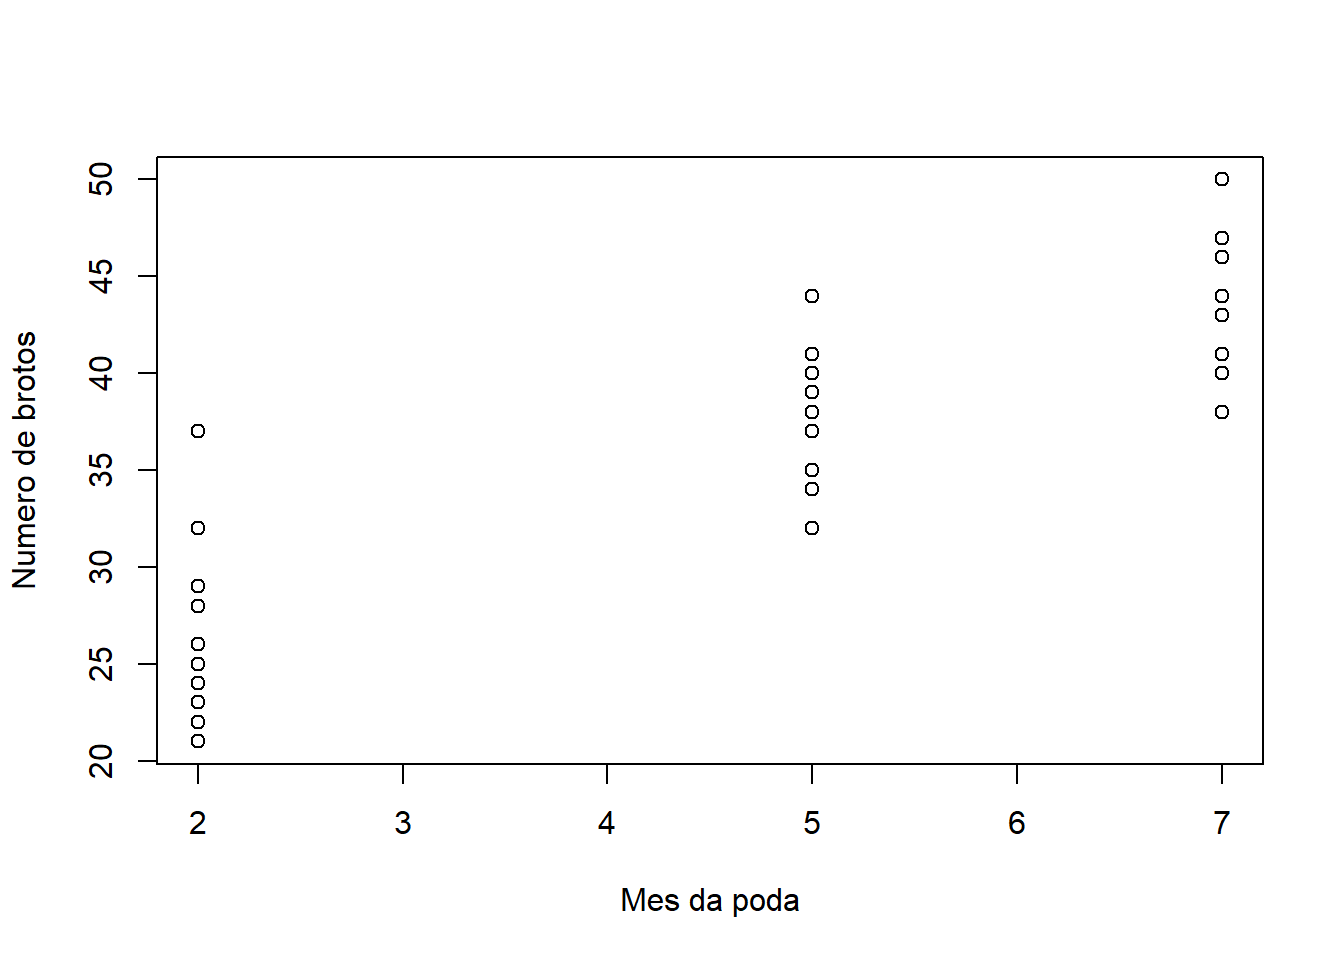
\includegraphics{bookdown_files/unnamed-chunk-47-1.png}

A interpretação de um gráfico de dispersão é bastante intuitiva e direta. Em geral, no eixo X (horizontal) coloca-se a variável que espera-se influenciar de alguma maneira a variável que está no eixo Y (vertical). A variável X é chamada de variável independente ou explicativa e a variável Y é chamada de variável dependente ou explicada.

Dessa maneira, analisa-se o quanto a variável do eixo X está influenciando a variável do eixo Y.

No exemplo apresentado acima, a variável mês de poda influencia positivamente o número de brotos. Uma vez que quanto maior o mês de poda, maior é o número de brotos. Neste caso, observa-se uma relação diretamente proporcional.

\hypertarget{boxplot-gruxe1fico-de-caixas}{%
\subsection{Boxplot: Gráfico de caixas}\label{boxplot-gruxe1fico-de-caixas}}

A função \texttt{boxplot()} é indicada para analisar uma variável categórica e outra variável contínua. Situação ideal, por exemplo, para verificar a influência de tratamentos qualitativos sobre uma variável de interesse. Ou ainda, avaliar o efeito do bloco sobre a variável de interesse.

\begin{Shaded}
\begin{Highlighting}[]
\NormalTok{exp.grafico =}\StringTok{ }\KeywordTok{read.csv}\NormalTok{(}\StringTok{"./data/Exemplo para Graficos.csv"}\NormalTok{, }\DataTypeTok{sep =} \StringTok{","}\NormalTok{, }\DataTypeTok{dec =} \StringTok{"."}\NormalTok{)}
\KeywordTok{boxplot}\NormalTok{(}\DataTypeTok{data =}\NormalTok{ exp.grafico, Brotos }\OperatorTok{~}\StringTok{ }\NormalTok{Bloco, }
        \DataTypeTok{xlab =} \StringTok{"Bloco"}\NormalTok{, }
        \DataTypeTok{ylab =} \StringTok{"Numero de brotos"}\NormalTok{)}
\end{Highlighting}
\end{Shaded}

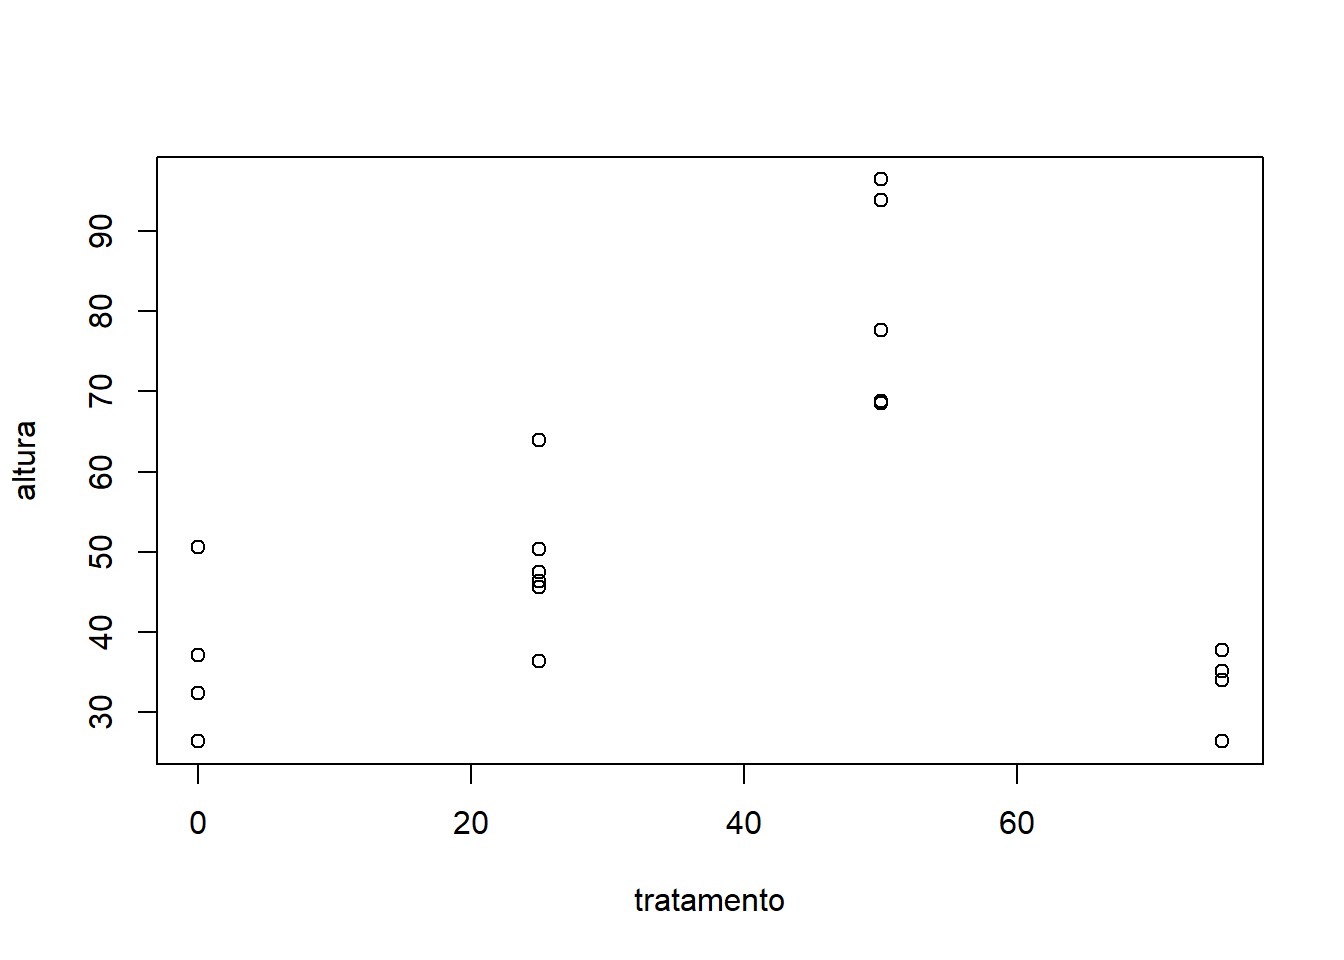
\includegraphics{bookdown_files/unnamed-chunk-48-1.png}

A interpretação do boxplot pode parecer complicada, já que este gráfico apresenta uma série de informações estatísticas em um único gráfico. Mas é justamente esta característica que o torna tão utilizado e tão importante.

A estrutura clássica do boxplot apresenta uma linha horizontal, dentro de uma caixa, sobreposta a uma linha vertical (do inglês \emph{whisker}, também conhecida como bigode).

A linha horizontal no interior da caixa indica a mediana, ou o segundo quartil. Os limites da caixa indicam o primeiro e o terceiro quartil. Os fios do bigode (ou \emph{whiskers}) indicam o máximo e o mínimo, excluindo \emph{outliers}. A função boxplot assume como outlier dados que estão acima ou abaixo de 1.5 vezes a distância inter-quartil. Estes pontos considerados \emph{outlier} serão marcados pontualmente no gráfico se estiverem presentes. No exemplo que apresentado acima, não houve a presença de \emph{outliers}.

Lembre-se! O gráfico criado com a função \texttt{boxplot()} não remove os \emph{outliers}, apenas exibe no gráfico. Assim, cabe a você a decisão de removê-los ou não.

\hypertarget{delineamento-inteiramente-casualizado}{%
\section{Delineamento inteiramente casualizado}\label{delineamento-inteiramente-casualizado}}

Este é sem dúvida o caso mais simples dos delineamentos experimentais. Aqui, o fenômeno de estudo se resume a apenas duas fontes de variação: uma fonte de variação conhecida, determinada pelo tratamento e uma fonte de variação desconhecida, determinada pelo resíduo.

\hypertarget{recapitulando}{%
\subsection{Recapitulando}\label{recapitulando}}

A análise começa pela determinação das somas de quadrados total, que é formada pela soma de quadrados do tratamento e pela soma de quadrados do resíduo. Uma vez obtidas as somas de quadrados, calculam-se os quadrados médios e o valor da estatística F. Se F calculado for superior ao F tabelado, assume-se que existe um efeito devido aos tratamentos, ao passo que se F calculado for inferior ao F tabelado, não há evidências suficientes para rejeitar a hipótese nula, aceitando-se a hipótese de que não existe efeito dos tratamentos.

Sendo o efeito dos tratamentos significativo, realiza-se o desdobramento por meio de um teste de médias, se os tratamentos forem qualitativos, ou por meio de uma análise de regressão se os tratamentos forem quantitativos.

\hypertarget{o-caso-balanceado}{%
\subsection{O caso balanceado}\label{o-caso-balanceado}}

Para exemplificar o caso balanceado, será analisado um estudo sobre a influência de três diferentes tipos de substrato no crescimento em altura de mudas. Cada tipo de substrato foi utilizado na germinação de 10 plantas. 90 dias após o semeio, as alturas das plântulas foram medidas e registradas numa planilha eletrônica. Os dados podem ser assim resumidos:

\begin{itemize}
\tightlist
\item
  Tratamento: 3 substratos
\item
  10 repetições
\item
  Variável de interesse: altura
\end{itemize}

Abaixo seguem as medições de altura tabuladas. Embora o R seja compatível com diversas extensões de planilhas eletrônicas, serão utilizados ao longo do livro arquivos em extensão \texttt{.csv}.

\begin{table}

\caption{\label{tab:unnamed-chunk-49}Dados de delineamento inteiramente casualizado}
\centering
\begin{tabular}[t]{l|r|r}
\hline
tratamento & rep & altura\\
\hline
Substrato 1 & 1 & 1.2\\
\hline
Substrato 1 & 2 & 8.6\\
\hline
Substrato 1 & 3 & 8.6\\
\hline
Substrato 1 & 4 & 3.7\\
\hline
Substrato 1 & 5 & 9.9\\
\hline
Substrato 1 & 6 & 2.5\\
\hline
Substrato 1 & 7 & 6.2\\
\hline
Substrato 1 & 8 & 6.2\\
\hline
Substrato 1 & 9 & 1.2\\
\hline
Substrato 1 & 10 & 3.7\\
\hline
Substrato 2 & 1 & 2.5\\
\hline
Substrato 2 & 2 & 8.6\\
\hline
Substrato 2 & 3 & 7.4\\
\hline
Substrato 2 & 4 & 6.2\\
\hline
Substrato 2 & 5 & 9.9\\
\hline
Substrato 2 & 6 & 2.5\\
\hline
Substrato 2 & 7 & 6.2\\
\hline
Substrato 2 & 8 & 6.2\\
\hline
Substrato 2 & 9 & 1.2\\
\hline
Substrato 2 & 10 & 3.7\\
\hline
Substrato 3 & 1 & 3.7\\
\hline
Substrato 3 & 2 & 9.9\\
\hline
Substrato 3 & 3 & 11.1\\
\hline
Substrato 3 & 4 & 7.4\\
\hline
Substrato 3 & 5 & 7.4\\
\hline
Substrato 3 & 6 & 3.7\\
\hline
Substrato 3 & 7 & 6.2\\
\hline
Substrato 3 & 8 & 8.6\\
\hline
Substrato 3 & 9 & 11.1\\
\hline
Substrato 3 & 10 & 11.1\\
\hline
\end{tabular}
\end{table}

O primeiro passo é importar o arquivo csv contendo o experimento para dentro do R. Esta tarefa pode ser realizada através do seguinte comando:

\begin{Shaded}
\begin{Highlighting}[]
\NormalTok{dic1 =}\StringTok{ }\KeywordTok{read.csv}\NormalTok{(}\StringTok{"./data/Experimento DIC 1.csv"}\NormalTok{)}
\end{Highlighting}
\end{Shaded}

Com a importação, cria-se um objeto chamado \texttt{dic1}, contendo os dados do experimento num formato de \texttt{dataframe}.

Antes de partir para a análise, é fundamental explorar os dados de forma gráfica para conhecer melhor as relações e antecipar o resultado da análise estatística. A construção do gráfico ajuda na compreensão do fenômeno estudado e na validação da análise estatística escolhida. Por se tratar de um experimento com o tratamento formado por níveis qualitativos, recomenda-se o uso do \texttt{boxplot()}.

\begin{Shaded}
\begin{Highlighting}[]
\KeywordTok{boxplot}\NormalTok{(}\DataTypeTok{data =}\NormalTok{ dic1, altura }\OperatorTok{~}\StringTok{ }\NormalTok{tratamento)}
\end{Highlighting}
\end{Shaded}

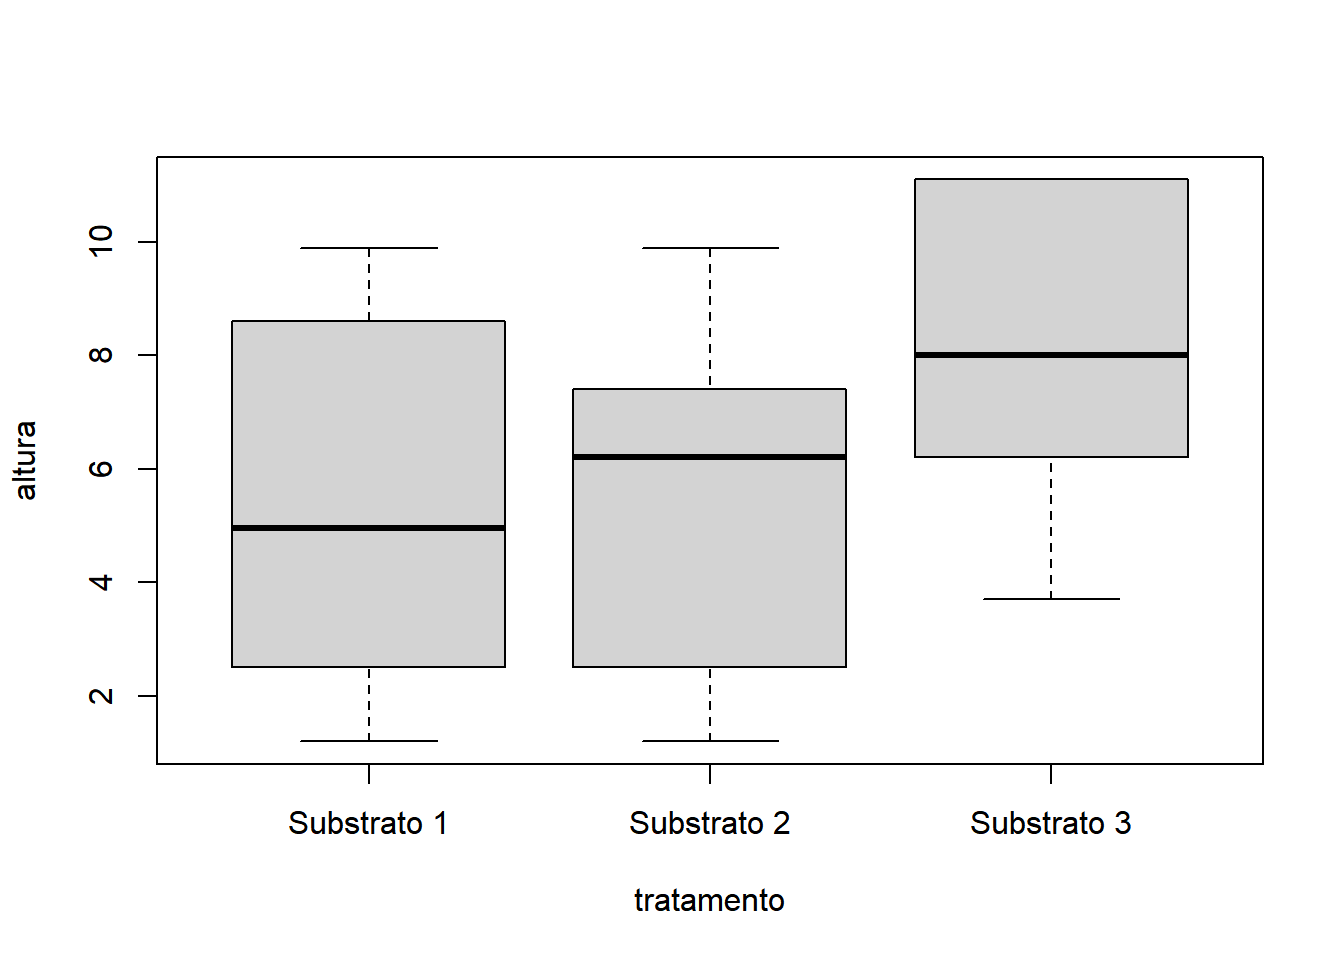
\includegraphics{bookdown_files/unnamed-chunk-51-1.png}

Pelo gráfico obtido, é razoável esperar que não haja diferenças significativas entre os tratamentos (3 substratos), pois existe uma grande sobreposição entre os interquartis dos substratos. Assim, espera-se que a análise estatística do experimento corrobore a conclusão empírica baseada no interpretação do gráfico.

Com a função \texttt{dic()} do pacote \texttt{ExpDes.pt} será possível realizar toda a análise de um experimento de delineamento inteiramente casualizado, inclusive o desdobramento caso o teste F seja significativo e o tratamento tenha três ou mais níveis.

Lembre-se que o pacote \texttt{ExpDes.pt} não faz parte da instalação padrão do R, e precisa ser adicionado à parte. A sintaxe básica da função \texttt{dic()} é:

\begin{Shaded}
\begin{Highlighting}[]
\KeywordTok{dic}\NormalTok{(trat, resp, }\DataTypeTok{quali =} \OtherTok{TRUE}\NormalTok{, }\DataTypeTok{mcomp =} \StringTok{"tukey"}\NormalTok{, }\DataTypeTok{sigT =} \FloatTok{0.05}\NormalTok{, }\DataTypeTok{sigF =} \FloatTok{0.05}\NormalTok{)}
\end{Highlighting}
\end{Shaded}

Neste experimento, não será necessário alterar nenhum parâmetro opcional, sendo então o comando construído da seguinte maneira:

\begin{Shaded}
\begin{Highlighting}[]
\KeywordTok{require}\NormalTok{(ExpDes.pt)}
\KeywordTok{dic}\NormalTok{(dic1}\OperatorTok{$}\NormalTok{tratamento, dic1}\OperatorTok{$}\NormalTok{altura)}
\end{Highlighting}
\end{Shaded}

\begin{verbatim}
## ------------------------------------------------------------------------
## Quadro da analise de variancia
## ------------------------------------------------------------------------
##            GL      SQ      QM     Fc    Pr>Fc
## Tratamento  2  49.299 24.6493 2.7908 0.079121
## Residuo    27 238.476  8.8324                
## Total      29 287.775                        
## ------------------------------------------------------------------------
## CV = 47.83 %
## 
## ------------------------------------------------------------------------
## Teste de normalidade dos residuos ( Shapiro-Wilk ) 
## Valor-p:  0.06889791 
## De acordo com o teste de Shapiro-Wilk a 5% de significancia, os residuos podem ser considerados normais.
## ------------------------------------------------------------------------
## 
## ------------------------------------------------------------------------
## Teste de homogeneidade de variancia 
## valor-p:  0.937449 
## De acordo com o teste de bartlett a 5% de significancia, as variancias podem ser consideradas homogeneas.
## ------------------------------------------------------------------------
## 
## De acordo com o teste F, as medias nao podem ser consideradas diferentes.
## ------------------------------------------------------------------------
##        Niveis Medias
## 1 Substrato 1   5.18
## 2 Substrato 2   5.44
## 3 Substrato 3   8.02
## ------------------------------------------------------------------------
\end{verbatim}

A primeira parte da análise é o quadro da variância que apresenta as fontes de variação com seus respectivos graus de liberdade, somas de quadrado e quadrados médio. Neste quadro também é apresentado o resultado do F calculado, que é a razão do quadrado médio do tratamento com o quadrado médio do resíduo.

No capítulo sobre a análise de variância, o quadro da ANOVA terminava com o F calculado, sendo seguido pela análise de uma tabela da estatística F para comparar o valor do F calculado com o valor de F tabelado. Nos softwares, não é necessário recorrer à tabela F, já que o \emph{p-valor} oferece uma interpretação direta da significância.

O \emph{p-valor} do experimento foi 0,079121, o que equivale à um grau de significância de 7,9\%. Sendo o nível de significância do experimento de 5\%, o \emph{p-valor} ficou acima da tolerância, indicando que o experimento não é significativo para um nível de 5\%. Obviamente, também não é significativo para um nível de 1\%.

Logo abaixo do quadro da ANOVA, é apresentado o coeficiente de variação do experimento (CV): 47,83\%. O CV é utilizado para medir a precisão do experimento, representado pelo o desvio-padrão expresso como porcentagem da média. A interpretação do CV é muito subjetiva e varia muito entre as áreas da ciência.

Outra informação importante antes de aceitar o resultado da ANOVA, é verificar se os resíduos apresentam normalidade. Esta é uma pressuposição importante, uma vez que valida a escolha do modelo teórico do DIC para explicar o fenômeno:

\[Y = \bar{Y} + TRAT + Erro\]

A não normalidade coloca em xeque o modelo teórico escolhido. Sendo então indicado a transformação dos dados e novo processamento da análise. A pressuposição deve então ser novamente verificada. Obtendo normalidade, os resultados obtidos com a variável transformada podem ser utilizados. Caso contrário, recomenda-se o uso de testes não paramétricos.

Neste exemplo, o teste de normalidade foi não significativo (\emph{p-valor} = 0,06) e portanto não há evidências para rejeitar a hipótese de normalidade dos resíduos. Lembre-se que a pressuposição de normalidade deve ser sempre analisada em relação aos resíduos, e não às variáveis. A variável apresentar normalidade não garante que os resíduos do modelo estatístico também apresentarão normalidade.

A última parte da saída apresenta o resultado do desdobramento caso o teste F seja significativo. Neste experimento, os tratamentos não são significativos e portanto, apresenta-se apenas a média de cada tratamento.

\hypertarget{outro-caso-balanceado}{%
\subsection{Outro caso balanceado}\label{outro-caso-balanceado}}

Neste exemplo, segue outro experimento em delineamento inteiramente casualizado, em que se avalia a resposta no desenvolvimento em altura das plantas de quatro níveis de um nutriente. Cada nível de nutriente foi repetido 6 vezes. Assim o experimento pode ser resumido como:

\begin{itemize}
\tightlist
\item
  Tratamento: 4 dosagens de um nutriente
\item
  6 repetições
\item
  Variável de interesse: altura
\end{itemize}

\begin{table}

\caption{\label{tab:unnamed-chunk-54}Dados de outro delineamento inteiramente casualizado}
\centering
\begin{tabular}[t]{r|r|r}
\hline
tratamento & rep & altura\\
\hline
0 & 1 & 32.3\\
\hline
0 & 2 & 50.6\\
\hline
0 & 3 & 50.6\\
\hline
0 & 4 & 38.8\\
\hline
0 & 5 & 37.1\\
\hline
0 & 6 & 26.3\\
\hline
25 & 1 & 46.3\\
\hline
25 & 2 & 50.3\\
\hline
25 & 3 & 47.5\\
\hline
25 & 4 & 45.6\\
\hline
25 & 5 & 63.9\\
\hline
25 & 6 & 36.3\\
\hline
50 & 1 & 68.5\\
\hline
50 & 2 & 93.9\\
\hline
50 & 3 & 96.5\\
\hline
50 & 4 & 77.7\\
\hline
50 & 5 & 77.7\\
\hline
50 & 6 & 68.8\\
\hline
75 & 1 & 26.3\\
\hline
75 & 2 & 40.3\\
\hline
75 & 3 & 37.7\\
\hline
75 & 4 & 35.1\\
\hline
75 & 5 & 33.9\\
\hline
75 & 6 & 26.3\\
\hline
\end{tabular}
\end{table}

O primeiro passo é importar o arquivo csv contendo os resultados do experimento para dentro do R. Esta tarefa pode ser realizada através do seguinte comando:

\begin{Shaded}
\begin{Highlighting}[]
\NormalTok{dic2 =}\StringTok{ }\KeywordTok{read.csv}\NormalTok{(}\StringTok{"./data/Experimento DIC 2.csv"}\NormalTok{)}
\end{Highlighting}
\end{Shaded}

Antes de chamar a análise estatística, recomenda-se explorar os dados graficamente. O gráfico permite verificar a tendência da variável altura em função das doses, além de verificar a possível ocorrência de \emph{outliers}. Por se tratar de um experimento de níveis quantitativos, o gráfico de dispersão é mais adequado:

\begin{Shaded}
\begin{Highlighting}[]
\KeywordTok{plot}\NormalTok{(}\DataTypeTok{data =}\NormalTok{ dic2, altura }\OperatorTok{~}\StringTok{ }\NormalTok{tratamento)}
\end{Highlighting}
\end{Shaded}

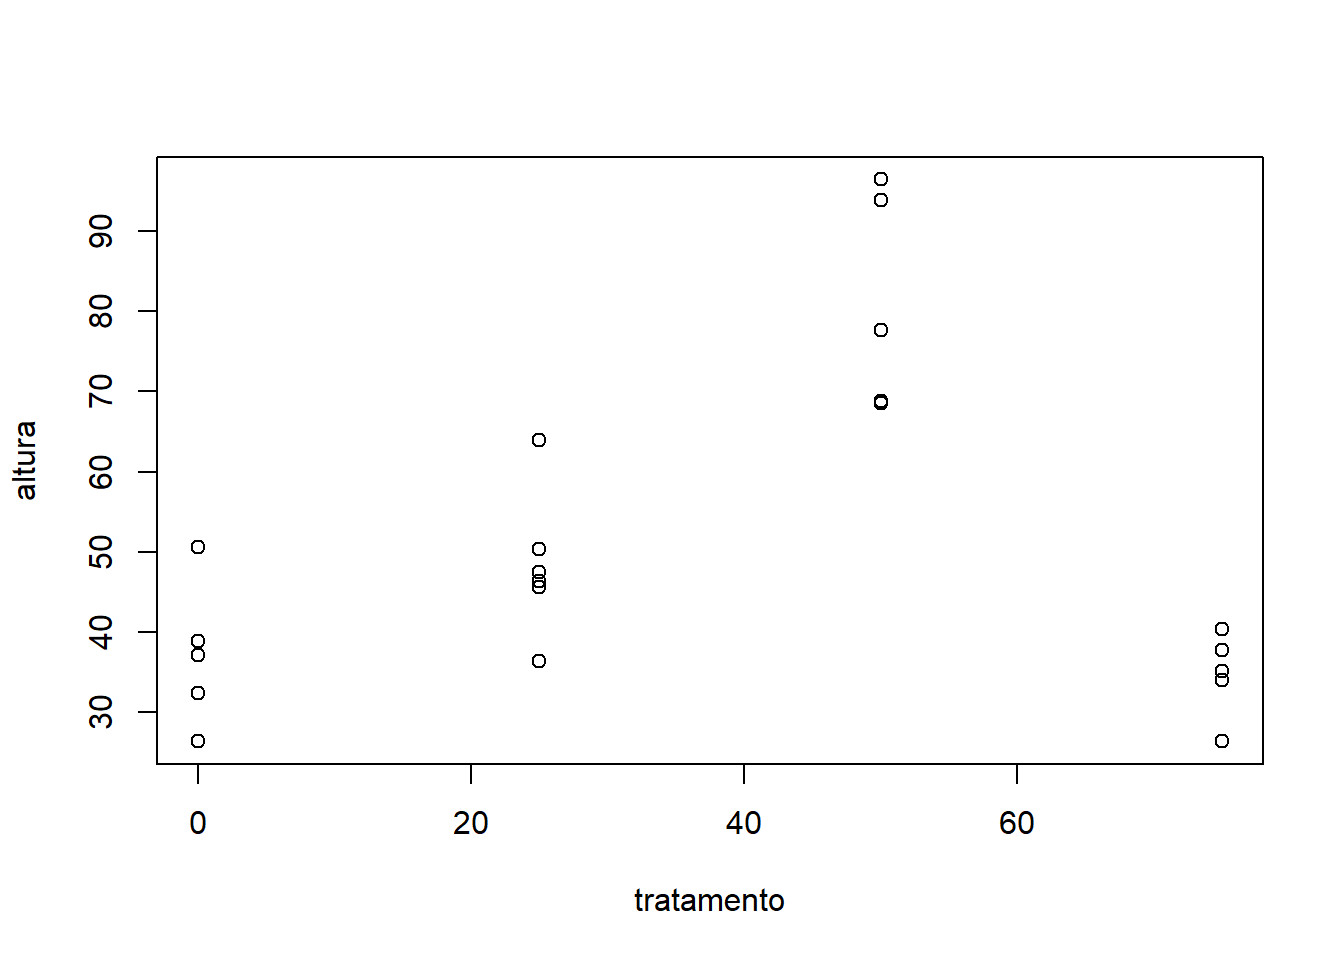
\includegraphics{bookdown_files/unnamed-chunk-56-1.png}

O gráfico indica que a dosagem de 50 apresenta um desenvolvimento em altura superior às demais dosagens. Outro ponto que fica claro com o gráfico, é que o tratamento tem um efeito quadrático sobre a altura. Por se tratar de um caso balanceado, a análise estatística pode ser realizada com a função \texttt{dic()} do pacote \texttt{ExpDes.pt}:

\begin{Shaded}
\begin{Highlighting}[]
\KeywordTok{require}\NormalTok{(ExpDes.pt)}
\KeywordTok{dic}\NormalTok{(dic2}\OperatorTok{$}\NormalTok{tratamento, dic2}\OperatorTok{$}\NormalTok{altura, }\DataTypeTok{quali =} \OtherTok{FALSE}\NormalTok{)}
\end{Highlighting}
\end{Shaded}

\begin{verbatim}
## ------------------------------------------------------------------------
## Quadro da analise de variancia
## ------------------------------------------------------------------------
##            GL     SQ      QM     Fc     Pr>Fc
## Tratamento  3 7970.8 2656.95 29.789 1.413e-07
## Residuo    20 1783.8   89.19                 
## Total      23 9754.7                         
## ------------------------------------------------------------------------
## CV = 18.76 %
## 
## ------------------------------------------------------------------------
## Teste de normalidade dos residuos ( Shapiro-Wilk ) 
## Valor-p:  0.1590112 
## De acordo com o teste de Shapiro-Wilk a 5% de significancia, os residuos podem ser considerados normais.
## ------------------------------------------------------------------------
## 
## ------------------------------------------------------------------------
## Teste de homogeneidade de variancia 
## valor-p:  0.5117623 
## De acordo com o teste de bartlett a 5% de significancia, as variancias podem ser consideradas homogeneas.
## ------------------------------------------------------------------------
## 
## Ajuste de modelos polinomiais de regressao
## ------------------------------------------------------------------------
## 
## Modelo Linear
## =========================================
##    Estimativa Erro.padrao   tc    valor.p
## -----------------------------------------
## b0  48.2233     3.2258    14.9493    0   
## b1   0.0566     0.0690    0.8206  0.4215 
## -----------------------------------------
## 
## R2 do modelo linear
## --------
## 0.007536
## --------
## 
## Analise de variancia do modelo linear
## ===========================================================
##                      GL     SQ         QM      Fc   valor.p
## -----------------------------------------------------------
## Efeito linear        1   60.0668    60.0668   0.67  0.42152
## Desvios de Regressao 2  7,910.7750 3,955.3870 44.35    0   
## Residuos             20 1,783.8380  89.1919                
## -----------------------------------------------------------
## ------------------------------------------------------------------------
## 
## Modelo quadratico
## =========================================
##    Estimativa Erro.padrao   tc    valor.p
## -----------------------------------------
## b0  34.1525     3.7579    9.0881     0   
## b1   1.7451     0.2414    7.2292     0   
## b2  -0.0225     0.0031    -7.2990    0   
## -----------------------------------------
## 
## R2 do modelo quadratico
## --------
## 0.603674
## --------
## 
## Analise de variancia do modelo quadratico
## ===========================================================
##                      GL     SQ         QM      Fc   valor.p
## -----------------------------------------------------------
## Efeito linear        1   60.0668    60.0668   0.67  0.42152
## Efeito quadratico    1  4,751.7200 4,751.7200 53.28    0   
## Desvios de Regressao 1  3,159.0540 3,159.0540 35.42  1e-05 
## Residuos             20 1,783.8380  89.1919                
## -----------------------------------------------------------
## ------------------------------------------------------------------------
## 
## Modelo cubico
## =========================================
##    Estimativa Erro.padrao   tc    valor.p
## -----------------------------------------
## b0  39.2833     3.8556    10.1888    0   
## b1  -1.4702     0.5917    -2.4846 0.0219 
## b2   0.1006     0.0209    4.8101  0.0001 
## b3  -0.0011     0.0002    -5.9514 0.00001
## -----------------------------------------
## 
## R2 do modelo cubico
## -
## 1
## -
## 
## Analise de variancia do modelo cubico
## ===========================================================
##                      GL     SQ         QM      Fc   valor.p
## -----------------------------------------------------------
## Efeito linear        1   60.0668    60.0668   0.67  0.42152
## Efeito quadratico    1  4,751.7200 4,751.7200 53.28    0   
## Efeito cubico        1  3,159.0540 3,159.0540 35.42  1e-05 
## Desvios de Regressao 0      0          0        0      1   
## Residuos             20 1,783.8380  89.1919                
## -----------------------------------------------------------
## ------------------------------------------------------------------------
\end{verbatim}

Note que o comando utilizado é muito semelhante ao exemplo anterior, com apenas uma diferença no parâmetro \texttt{quali}. Neste experimento, utiliza-se o parâmetro como \texttt{FALSE} por se tratar de um experimento com tratamento quantitativo.

O modelo estatístico pode ser aceito uma vez que não há evidências para rejeitar a hipótese de normalidade dos resíduos e homogeneidade de variâncias. Desta forma, pode-se dar sequência na interpretação dos resultados da análise do experimento.

Os tratamentos podem ser considerados significativos já que seu \emph{p-valor} é inferior a 1\%. O desdobramento do tratamento é realizado através de um teste de regressão, já que os níveis do tratamento são quantitativos e deseja-se obter uma equação de regressão que forneça a dose que proporciona a maior altura.

Como padrão, a função \texttt{dic()} desdobra os níveis do tratamento em três modelos: linear, quadrático e cúbico. Pelo gráfico de dispersão criado na fase de exploração dos dados, espera-se que o modelo quadrático seja o mais adequado para representação do experimento.

Com base nos resultados do desdobramento, nota-se que o modelo linear e cúbico são claramente inadequados. No caso do modelo linear, o \emph{p-valor} indica não significância do efeito linear, reforçado pelo coeficiente de determinação próximo a zero. O efeito cúbico, também foi inadequado pela falta de graus de liberdade. Como experimento analisado conta apenas com 4 níveis no tratamento, não sobra graus de liberdade para o resíduo. O modelo quadrático, por sua vez, apresenta um efeito significativo frente à análise de variância, tanto do efeito quanto dos coeficientes. O coeficiente de determinação de 60,36\% também indica um ajuste satisfatório.

A dose ótima do nutriente é de 38,8 gramas, indicado pelo ponto de máximo do modelo quadrático ajustado aos níveis analisados. Cuidado com extrapolações, uma vez que o experimento não contempla doses fora do intervalo analisado.

\hypertarget{o-caso-desbalanceado}{%
\subsection{O caso desbalanceado}\label{o-caso-desbalanceado}}

Experimentos desbalanceados são muito comuns na área das ciências agrárias. Isto ocorre principalmente devido à perda unidades experimentais devido à contaminação, morte ou eventos não previstos. Veja o experimento em delineamento inteiramente casualizado, em que se avalia a resposta no desenvolvimento em altura das plantas de quatro níveis de um nutriente. Cada nível de nutriente foi repetido 6 vezes.

\begin{itemize}
\tightlist
\item
  Tratamento: 4 dosagens de um nutriente
\item
  6 repetições
\item
  Variável de interesse: altura
\end{itemize}

No entanto, perceba que duas medições foram perdidas por morte das plantas:

\begin{itemize}
\tightlist
\item
  dose 0 repetição 4
\item
  dose 75 repetição 2
\end{itemize}

\begin{table}

\caption{\label{tab:unnamed-chunk-58}Dados de outro delineamento inteiramente casualizado, porém neste caso desbalanceado}
\centering
\begin{tabular}[t]{r|r|r}
\hline
tratamento & rep & altura\\
\hline
0 & 1 & 32.3\\
\hline
0 & 2 & 50.6\\
\hline
0 & 3 & 50.6\\
\hline
0 & 5 & 37.1\\
\hline
0 & 6 & 26.3\\
\hline
25 & 1 & 46.3\\
\hline
25 & 2 & 50.3\\
\hline
25 & 3 & 47.5\\
\hline
25 & 4 & 45.6\\
\hline
25 & 5 & 63.9\\
\hline
25 & 6 & 36.3\\
\hline
50 & 1 & 68.5\\
\hline
50 & 2 & 93.9\\
\hline
50 & 3 & 96.5\\
\hline
50 & 4 & 77.7\\
\hline
50 & 5 & 77.7\\
\hline
50 & 6 & 68.8\\
\hline
75 & 1 & 26.3\\
\hline
75 & 3 & 37.7\\
\hline
75 & 4 & 35.1\\
\hline
75 & 5 & 33.9\\
\hline
75 & 6 & 26.3\\
\hline
\end{tabular}
\end{table}

O primeiro passo é importar o arquivo contendo os resultados do experimento para dentro do R. Esta tarefa pode ser realizada através do seguinte comando:

\begin{Shaded}
\begin{Highlighting}[]
\NormalTok{dic3 =}\StringTok{ }\KeywordTok{read.csv}\NormalTok{(}\StringTok{"./data/Experimento DIC 3.csv"}\NormalTok{)}
\end{Highlighting}
\end{Shaded}

Antes de chamar a análise estatística, recomenda-se explorar os dados graficamente. Por se tratar de um tratamento de níveis quantitativos, o gráfico de dispersão é mais adequado:

\begin{Shaded}
\begin{Highlighting}[]
\KeywordTok{plot}\NormalTok{(}\DataTypeTok{data =}\NormalTok{ dic3, altura }\OperatorTok{~}\StringTok{ }\NormalTok{tratamento)}
\end{Highlighting}
\end{Shaded}

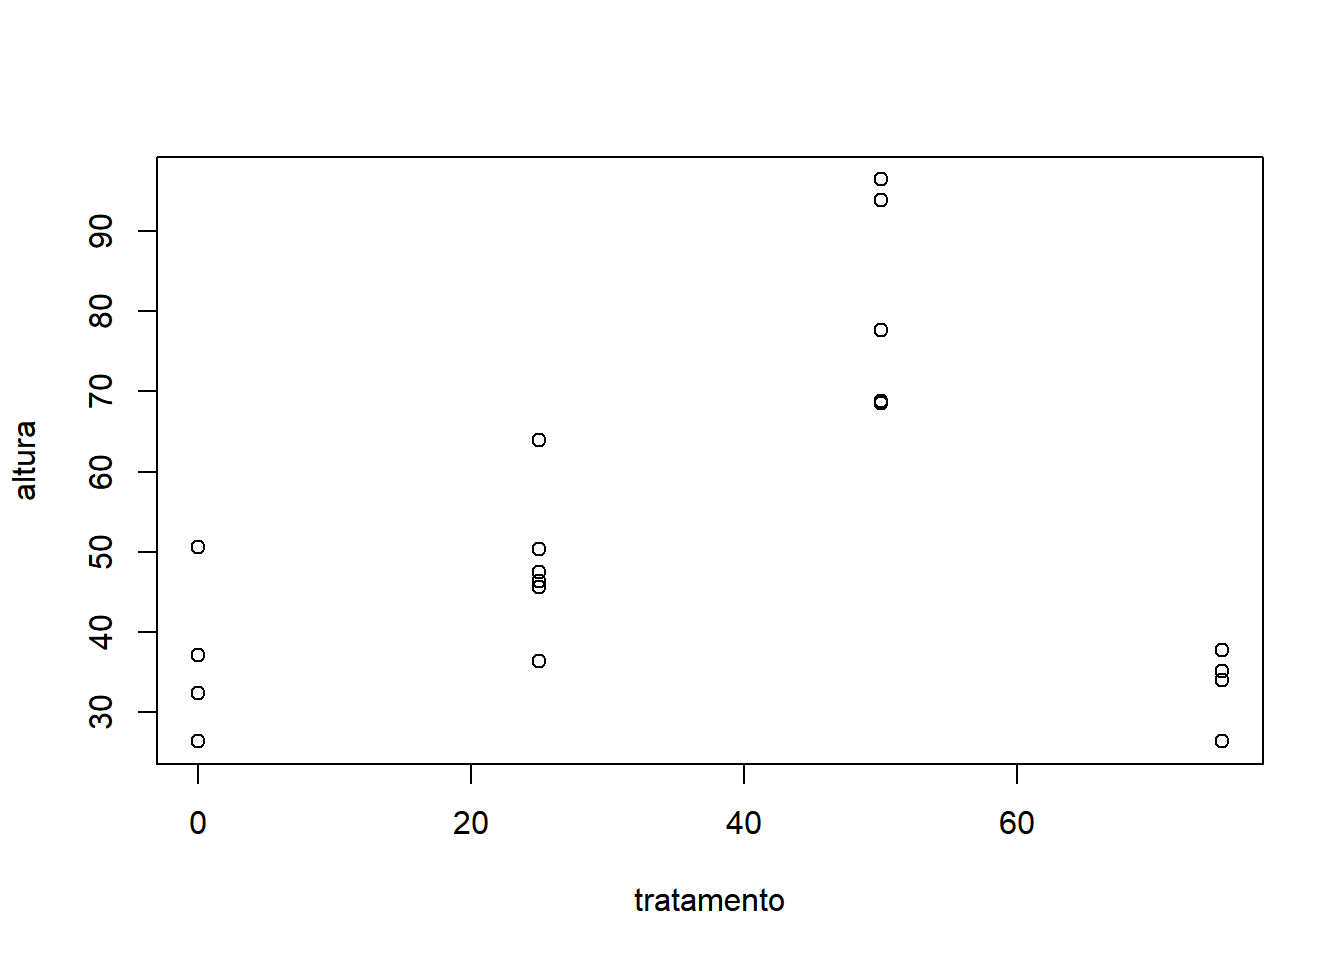
\includegraphics{bookdown_files/unnamed-chunk-60-1.png}

Mesmo se tratando de um experimento desbalanceado, por se tratar de um DIC e consequentemente não existir interações a serem calculadas, pode-se utilizar a ANOVA Tipo I. Com relação aos parâmetros opcionais, apenas o parâmetro \texttt{quali} precisa ser alterado para \texttt{FALSE}, por se tratar tratamento quantitativo:

\begin{Shaded}
\begin{Highlighting}[]
\KeywordTok{require}\NormalTok{(ExpDes.pt)}
\KeywordTok{dic}\NormalTok{(dic3}\OperatorTok{$}\NormalTok{tratamento, dic3}\OperatorTok{$}\NormalTok{altura, }\DataTypeTok{quali =} \OtherTok{FALSE}\NormalTok{)}
\end{Highlighting}
\end{Shaded}

\begin{verbatim}
## ------------------------------------------------------------------------
## Quadro da analise de variancia
## ------------------------------------------------------------------------
##            GL     SQ      QM     Fc      Pr>Fc
## Tratamento  3 7775.1 2591.69 27.056 6.8921e-07
## Residuo    18 1724.2   95.79                  
## Total      21 9499.3                          
## ------------------------------------------------------------------------
## CV = 19.07 %
## 
## ------------------------------------------------------------------------
## Teste de normalidade dos residuos ( Shapiro-Wilk ) 
## Valor-p:  0.1497467 
## De acordo com o teste de Shapiro-Wilk a 5% de significancia, os residuos podem ser considerados normais.
## ------------------------------------------------------------------------
## 
## ------------------------------------------------------------------------
## Teste de homogeneidade de variancia 
## valor-p:  0.4610355 
## De acordo com o teste de bartlett a 5% de significancia, as variancias podem ser consideradas homogeneas.
## ------------------------------------------------------------------------
## 
## Ajuste de modelos polinomiais de regressao
## ------------------------------------------------------------------------
## 
## Modelo Linear
## =========================================
##    Estimativa Erro.padrao   tc    valor.p
## -----------------------------------------
## b0  48.9626     3.5785    13.6823    0   
## b1   0.0631     0.0775    0.8134  0.4266 
## -----------------------------------------
## 
## R2 do modelo linear
## --------
## 0.008151
## --------
## 
## Analise de variancia do modelo linear
## ===========================================================
##                      GL     SQ         QM      Fc   valor.p
## -----------------------------------------------------------
## Efeito linear        1   63.3741    63.3741   0.66  0.42662
## Desvios de Regressao 2  7,711.6930 3,855.8460 40.25    0   
## Residuos             18 1,724.1970  95.7887                
## -----------------------------------------------------------
## ------------------------------------------------------------------------
## 
## Modelo quadratico
## =========================================
##    Estimativa Erro.padrao   tc    valor.p
## -----------------------------------------
## b0  33.2553     4.2463    7.8316     0   
## b1   1.7909     0.2631    6.8063     0   
## b2  -0.0230     0.0034    -6.8717    0   
## -----------------------------------------
## 
## R2 do modelo quadratico
## --------
## 0.589904
## --------
## 
## Analise de variancia do modelo quadratico
## ===========================================================
##                      GL     SQ         QM      Fc   valor.p
## -----------------------------------------------------------
## Efeito linear        1   63.3741    63.3741   0.66  0.42662
## Efeito quadratico    1  4,523.1710 4,523.1710 47.22    0   
## Desvios de Regressao 1  3,188.5220 3,188.5220 33.29  2e-05 
## Residuos             18 1,724.1970  95.7887                
## -----------------------------------------------------------
## ------------------------------------------------------------------------
## 
## Modelo cubico
## =========================================
##    Estimativa Erro.padrao   tc    valor.p
## -----------------------------------------
## b0  39.3800     4.3770    8.9971     0   
## b1  -1.4961     0.6275    -2.3840 0.0283 
## b2   0.1019     0.0219    4.6503  0.0002 
## b3  -0.0011     0.0002    -5.7695 0.00002
## -----------------------------------------
## 
## R2 do modelo cubico
## -
## 1
## -
## 
## Analise de variancia do modelo cubico
## ===========================================================
##                      GL     SQ         QM      Fc   valor.p
## -----------------------------------------------------------
## Efeito linear        1   63.3741    63.3741   0.66  0.42662
## Efeito quadratico    1  4,523.1710 4,523.1710 47.22    0   
## Efeito cubico        1  3,188.5220 3,188.5220 33.29  2e-05 
## Desvios de Regressao 0      0          0        0      1   
## Residuos             18 1,724.1970  95.7887                
## -----------------------------------------------------------
## ------------------------------------------------------------------------
\end{verbatim}

\hypertarget{delineamento-casualizado-em-blocos}{%
\section{Delineamento casualizado em blocos}\label{delineamento-casualizado-em-blocos}}

Nos experimentos casualizados em blocos (DBC), além do tratamento, uma segunda fonte de variação controlada é inserida no modelo e é denominada de bloco. O bloco é inserido pelo analista para controlar uma variação conhecida do ambiente, como por exemplo tipo de solo, insolação e outros. Assim a ANOVA contará com três fontes de variação: duas fontes de variação conhecidas (tratamento e bloco), e uma fonte de variação desconhecida (resíduo).

Vale destacar, que no DBC, não há interesse pela interação do bloco com o tratamento, sendo o bloco apenas para controlar uma possível variação sobre os tratamentos induzida por uma possível variação do ambiente. O modelo estatístico do delineamento casualizado em blocos é:

\[Y = \bar{Y} + BLOCO + TRAT + Erro\]

A análise começa pela determinação das somas de quadrados total, composta pela soma de quadrado do tratamento, pela soma de quadrado do bloco e pela soma de quadrado do resíduo. Em seguida, calculam-se os quadrados médios do tratamento e do resíduo e o valor da estatística F. Se F calculado for superior ao F tabelado, assume-se que existe um efeito devido aos tratamentos, ao passo que se F calculado for inferior ao F tabelado, não há evidências suficientes para rejeitar a hipótese nula, aceitando-se a hipótese de que não existe efeito dos tratamentos.

Embora em alguns softwares o teste F para o bloco seja realizado, o mesmo não é necessário. A utilidade do bloco é apenas isolar uma possível variação atribuída ao ambiente. Uma vez que tenha optado pelo uso do bloco, é irrelevante encontrar sua significância (ou não significância). Sendo o efeito dos tratamentos significativo, realiza-se o desdobramento do efeito dos tratamentos por meio de um teste de médias, se os tratamentos forem qualitativos, ou por meio de uma análise de regressão se os tratamentos forem quantitativos.

Para a análise de experimentos casualizados em blocos, como não há no modelo estatístico a influência da interação, utiliza-se o pacote \texttt{ExpDes.pt} tanto para o caso balanceado, quanto para o desbalanceado.

\hypertarget{o-caso-balanceado-1}{%
\subsection{O caso balanceado}\label{o-caso-balanceado-1}}

Para exemplificar o caso balanceado, será analisado um estudo sobre a influência de duas intensidades de desbaste no diâmetro de árvores. Os desbastes foram repetidos em 4 parcelas para cada um dos cinco blocos. Os blocos foram considerados para isolar o efeito dos diferentes tipos de solo. Os dados podem ser resumidos através dos seguintes tópicos:

\begin{itemize}
\tightlist
\item
  Tratamento: 2 intensidades de desbaste (30\% e 50\%)
\item
  5 Blocos
\item
  4 repetições
\item
  Variável de interesse: diâmetro
\end{itemize}

\begin{table}

\caption{\label{tab:unnamed-chunk-62}Dados de delineamento casualizado em blocos}
\centering
\begin{tabular}[t]{r|r|r|r}
\hline
desbaste & bloco & rep & diametro\\
\hline
30 & 1 & 1 & 28.37041\\
\hline
30 & 1 & 2 & 29.28010\\
\hline
30 & 1 & 3 & 30.84926\\
\hline
30 & 1 & 4 & 27.89227\\
\hline
30 & 2 & 1 & 20.38856\\
\hline
30 & 2 & 2 & 21.47290\\
\hline
30 & 2 & 3 & 24.39744\\
\hline
30 & 2 & 4 & 24.65861\\
\hline
30 & 3 & 1 & 23.79856\\
\hline
30 & 3 & 2 & 25.69388\\
\hline
30 & 3 & 3 & 24.45922\\
\hline
30 & 3 & 4 & 27.94071\\
\hline
30 & 4 & 1 & 28.05501\\
\hline
30 & 4 & 2 & 26.42934\\
\hline
30 & 4 & 3 & 23.09124\\
\hline
30 & 4 & 4 & 22.54273\\
\hline
30 & 5 & 1 & 32.73052\\
\hline
30 & 5 & 2 & 29.17538\\
\hline
30 & 5 & 3 & 29.94747\\
\hline
30 & 5 & 4 & 29.35810\\
\hline
50 & 1 & 1 & 31.20701\\
\hline
50 & 1 & 2 & 40.85273\\
\hline
50 & 1 & 3 & 33.66891\\
\hline
50 & 1 & 4 & 33.15001\\
\hline
50 & 2 & 1 & 34.03869\\
\hline
50 & 2 & 2 & 36.24517\\
\hline
50 & 2 & 3 & 35.49081\\
\hline
50 & 2 & 4 & 31.58952\\
\hline
50 & 3 & 1 & 31.92634\\
\hline
50 & 3 & 2 & 28.82107\\
\hline
50 & 3 & 3 & 32.18963\\
\hline
50 & 3 & 4 & 31.55686\\
\hline
50 & 4 & 1 & 31.11534\\
\hline
50 & 4 & 2 & 31.05093\\
\hline
50 & 4 & 3 & 34.69215\\
\hline
50 & 4 & 4 & 32.95378\\
\hline
50 & 5 & 1 & 25.26880\\
\hline
50 & 5 & 2 & 30.48375\\
\hline
50 & 5 & 3 & 31.73922\\
\hline
50 & 5 & 4 & 26.21619\\
\hline
\end{tabular}
\end{table}

O primeiro passo é importar o arquivo do experimento para dentro do R. Esta tarefa pode ser realizada através do seguinte comando:

\begin{Shaded}
\begin{Highlighting}[]
\NormalTok{dbc1 =}\StringTok{ }\KeywordTok{read.csv}\NormalTok{(}\StringTok{"./data/Experimento DBC 1.csv"}\NormalTok{)}
\end{Highlighting}
\end{Shaded}

Antes de partir para a análise, é fundamental explorar os dados de forma gráfica para conhecer melhor os dados e antecipar o resultado da análise estatística. A construção do gráfico ajuda na compreensão do fenômeno estudado e na validação da análise estatística escolhida. Por se tratar de um experimento com o tratamento formado por níveis quantitativos, porém com apenas dois níveis, recomenda-se o uso do \texttt{boxplot()}.

\begin{Shaded}
\begin{Highlighting}[]
\KeywordTok{boxplot}\NormalTok{(}\DataTypeTok{data =}\NormalTok{ dbc1, diametro }\OperatorTok{~}\StringTok{ }\NormalTok{desbaste}\OperatorTok{/}\NormalTok{bloco)}
\end{Highlighting}
\end{Shaded}

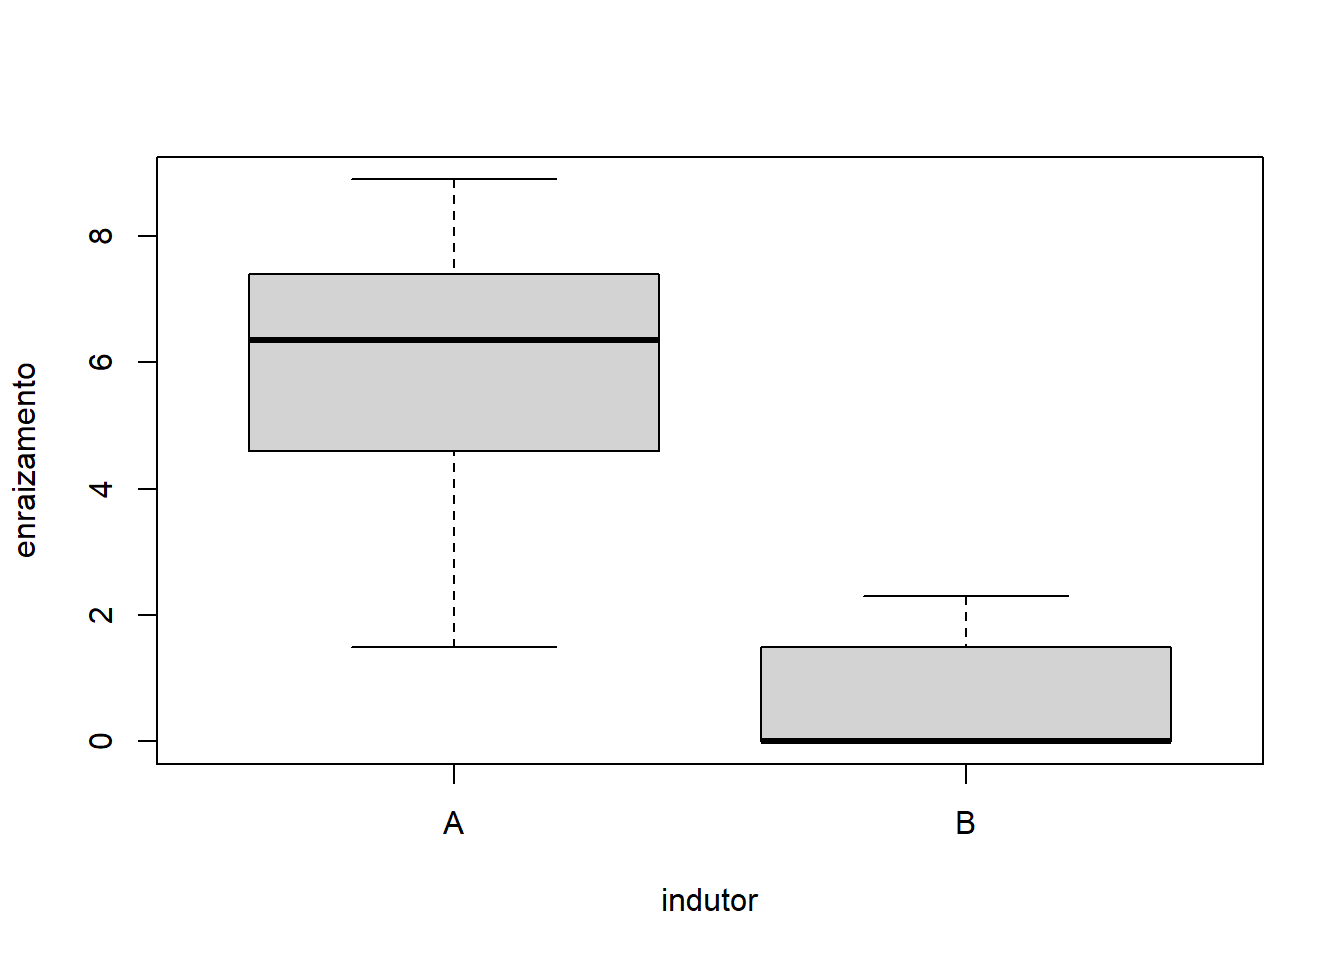
\includegraphics{bookdown_files/unnamed-chunk-64-1.png}

Note que os rótulo do eixo X são compostos pela união do desbaste e do bloco. Pode ser que dependendo do espaço disponível alguns rótulos sejam omitidos, mas ele devem ser lidos alternadamente, uma caixa para 30.1, outra para 50.1, depois 30.2, seguido de 50.2 e assim por diante.

Os tratamentos podem ser analisados isoladamente em relação a cada bloco, utilizando um filtro para escolher qual bloco considerar.

\begin{enumerate}
\def\labelenumi{\arabic{enumi}.}
\tightlist
\item
  Para bloco igual a 1:
\end{enumerate}

\begin{Shaded}
\begin{Highlighting}[]
\KeywordTok{boxplot}\NormalTok{(}\DataTypeTok{data =}\NormalTok{ dbc1[dbc1}\OperatorTok{$}\NormalTok{bloco }\OperatorTok{==}\StringTok{ }\DecValTok{1}\NormalTok{,], diametro}\OperatorTok{~}\NormalTok{desbaste}\OperatorTok{/}\NormalTok{bloco)}
\end{Highlighting}
\end{Shaded}

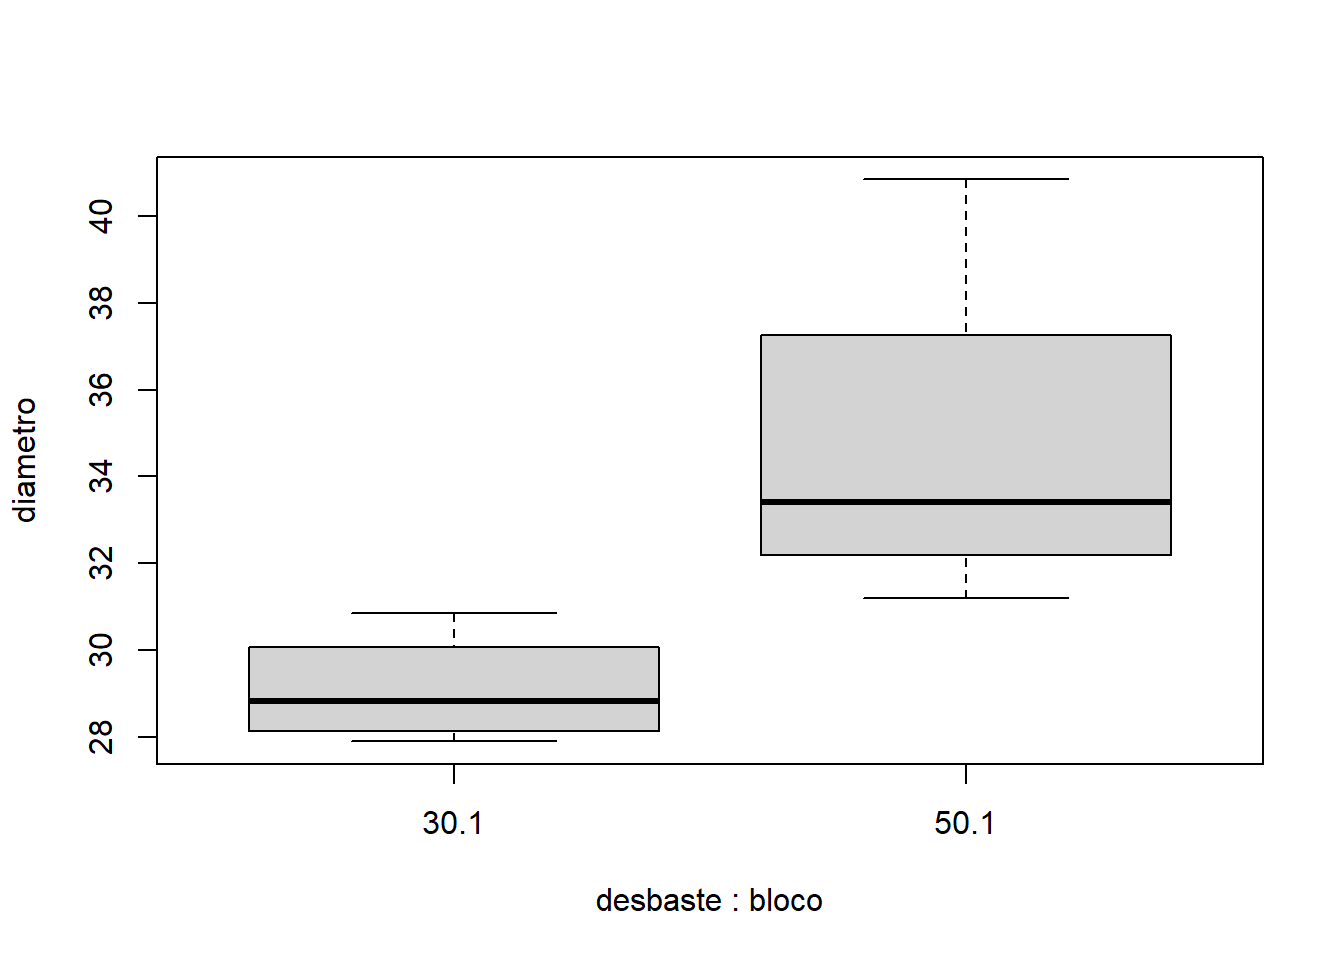
\includegraphics{bookdown_files/unnamed-chunk-65-1.png}

\begin{enumerate}
\def\labelenumi{\arabic{enumi}.}
\setcounter{enumi}{1}
\tightlist
\item
  Para bloco igual a 2:
\end{enumerate}

\begin{Shaded}
\begin{Highlighting}[]
\KeywordTok{boxplot}\NormalTok{(}\DataTypeTok{data =}\NormalTok{ dbc1[dbc1}\OperatorTok{$}\NormalTok{bloco }\OperatorTok{==}\StringTok{ }\DecValTok{2}\NormalTok{,], diametro}\OperatorTok{~}\NormalTok{desbaste}\OperatorTok{/}\NormalTok{bloco)}
\end{Highlighting}
\end{Shaded}

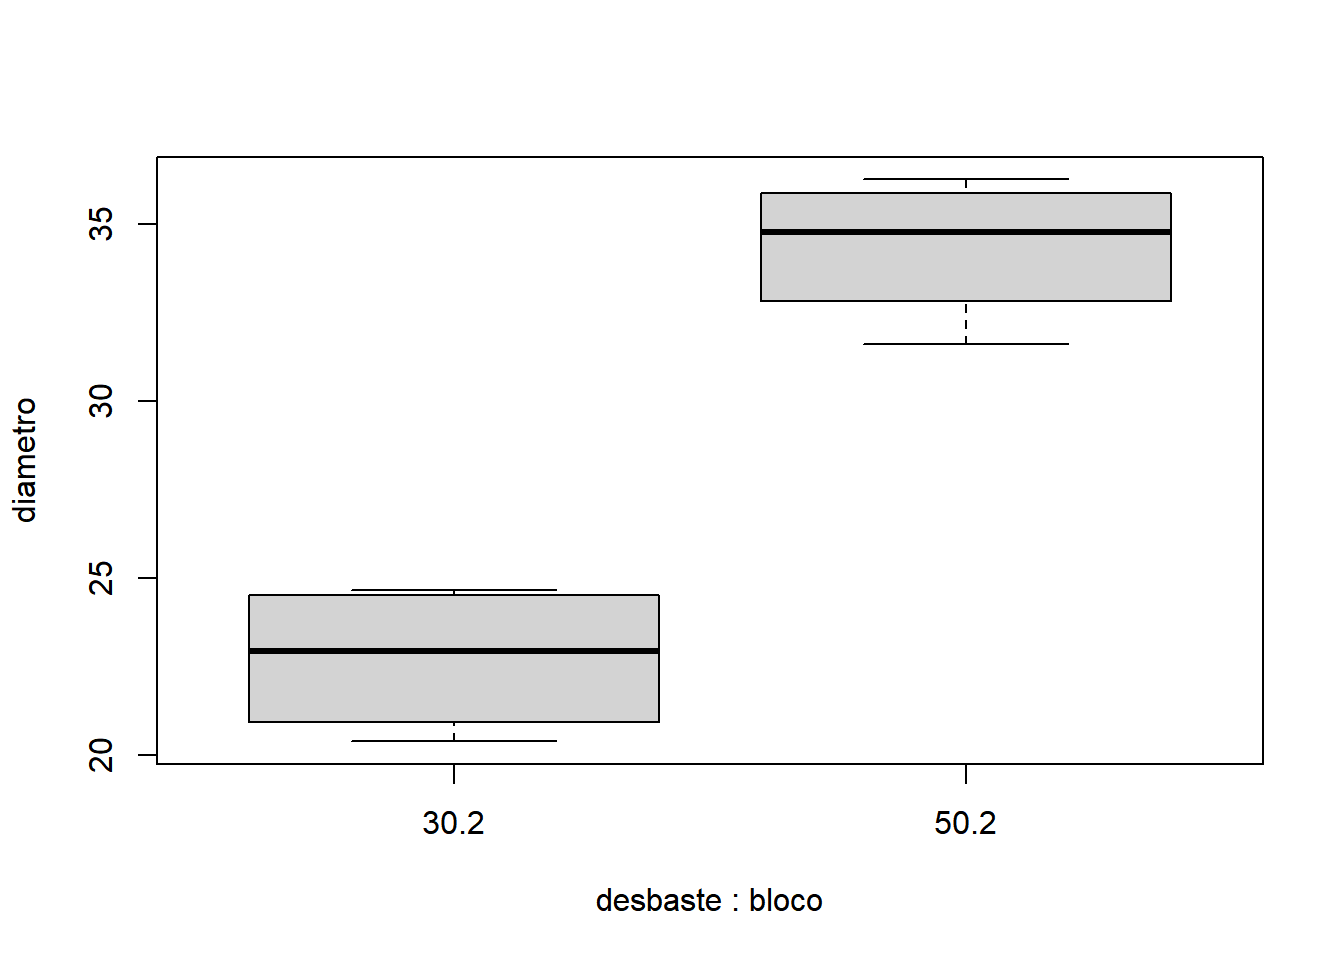
\includegraphics{bookdown_files/unnamed-chunk-66-1.png}

\begin{enumerate}
\def\labelenumi{\arabic{enumi}.}
\setcounter{enumi}{2}
\tightlist
\item
  Para bloco igual a 3:
\end{enumerate}

\begin{Shaded}
\begin{Highlighting}[]
\KeywordTok{boxplot}\NormalTok{(}\DataTypeTok{data =}\NormalTok{ dbc1[dbc1}\OperatorTok{$}\NormalTok{bloco }\OperatorTok{==}\StringTok{ }\DecValTok{3}\NormalTok{,], diametro}\OperatorTok{~}\NormalTok{desbaste}\OperatorTok{/}\NormalTok{bloco)}
\end{Highlighting}
\end{Shaded}

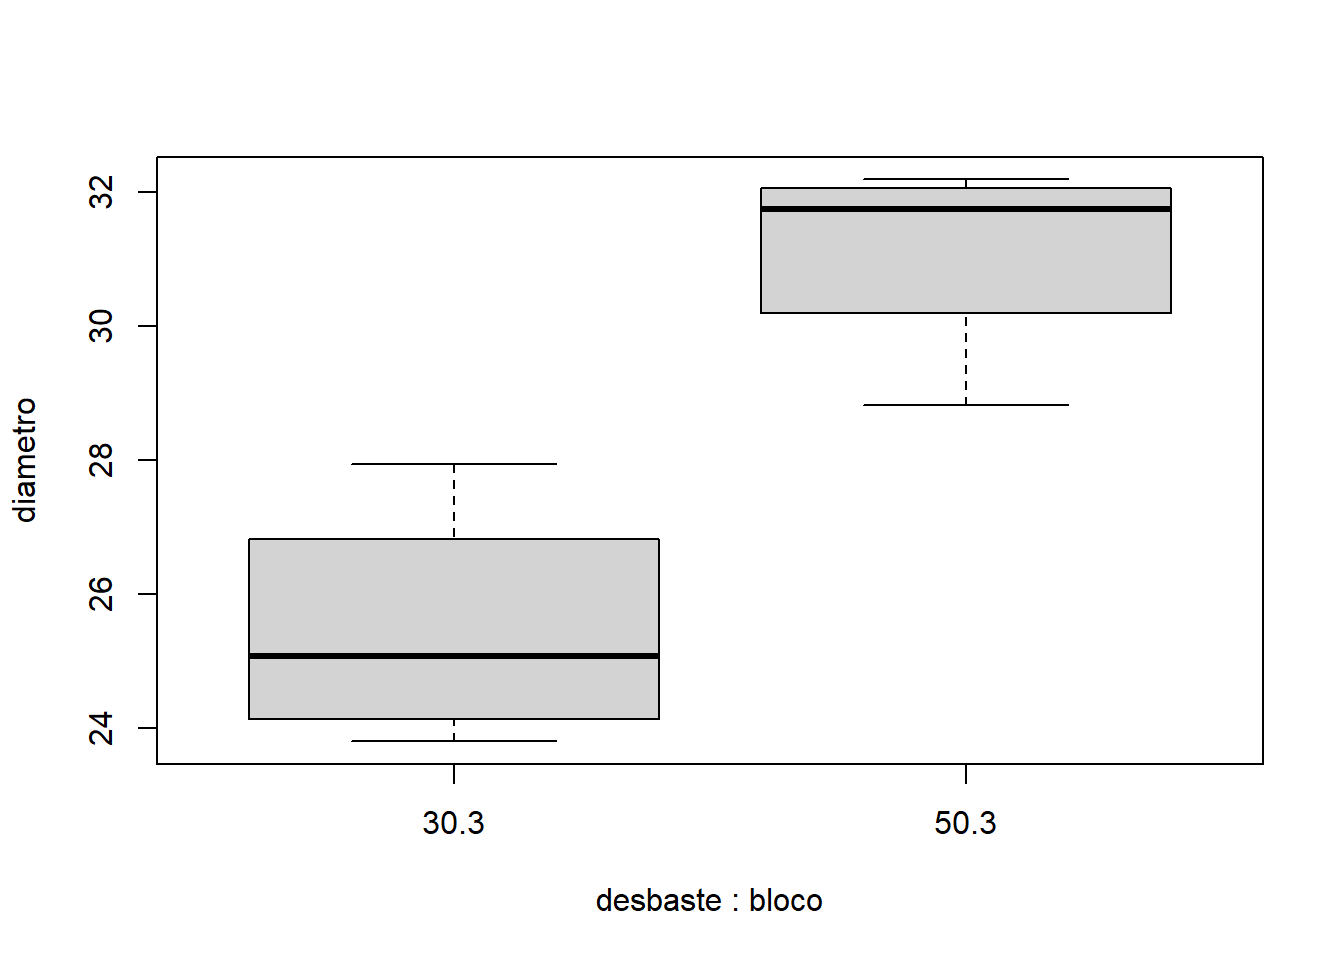
\includegraphics{bookdown_files/unnamed-chunk-67-1.png}

\begin{enumerate}
\def\labelenumi{\arabic{enumi}.}
\setcounter{enumi}{3}
\tightlist
\item
  Para bloco igual a 4:
\end{enumerate}

\begin{Shaded}
\begin{Highlighting}[]
\KeywordTok{boxplot}\NormalTok{(}\DataTypeTok{data =}\NormalTok{ dbc1[dbc1}\OperatorTok{$}\NormalTok{bloco }\OperatorTok{==}\StringTok{ }\DecValTok{4}\NormalTok{,], diametro}\OperatorTok{~}\NormalTok{desbaste}\OperatorTok{/}\NormalTok{bloco)}
\end{Highlighting}
\end{Shaded}

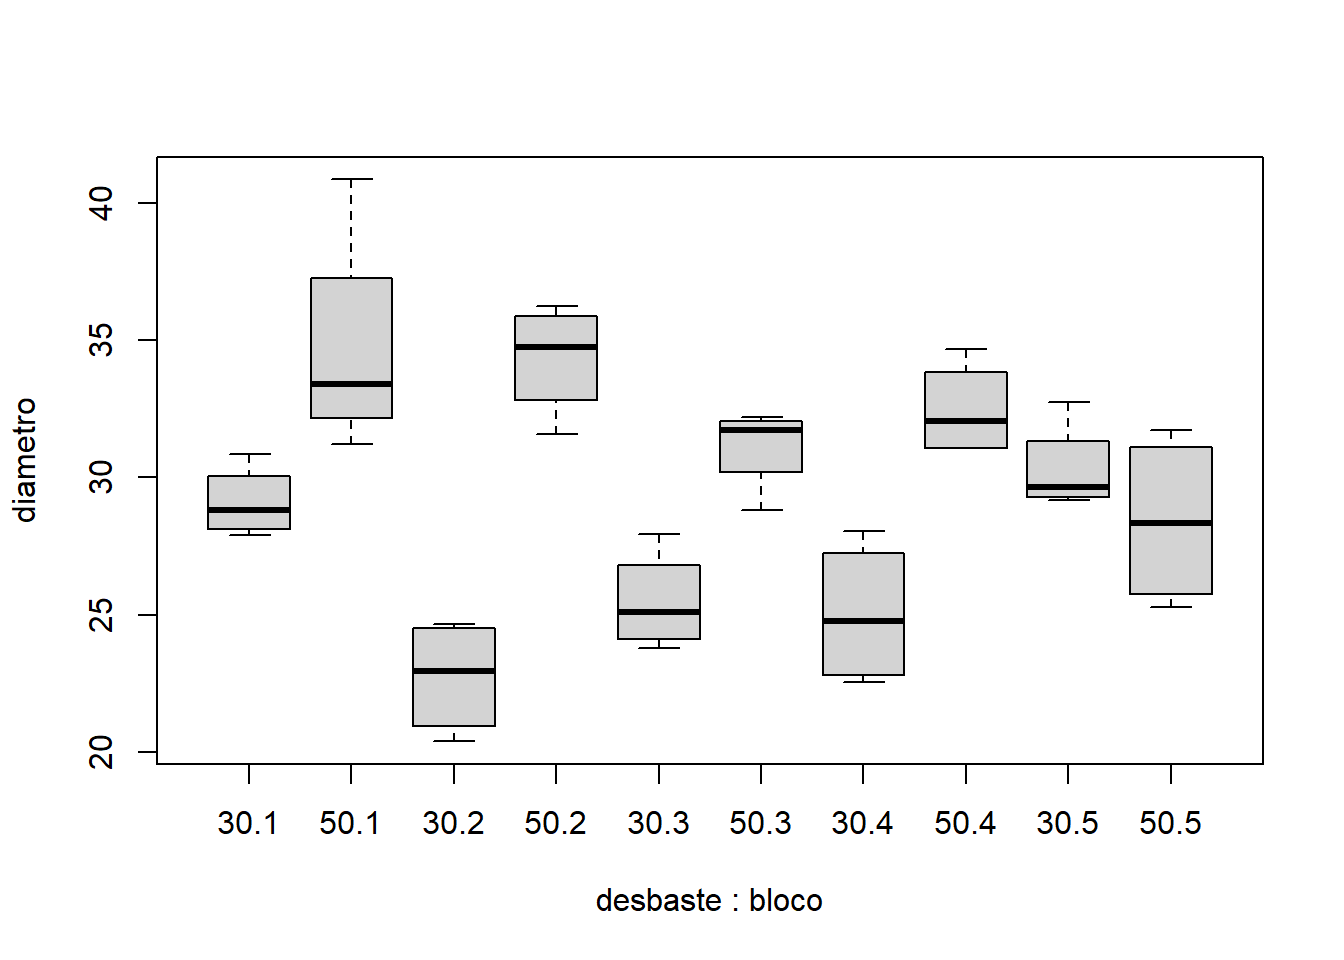
\includegraphics{bookdown_files/unnamed-chunk-68-1.png}

\begin{enumerate}
\def\labelenumi{\arabic{enumi}.}
\setcounter{enumi}{4}
\tightlist
\item
  Para bloco igual a 5:
\end{enumerate}

\begin{Shaded}
\begin{Highlighting}[]
\KeywordTok{boxplot}\NormalTok{(}\DataTypeTok{data =}\NormalTok{ dbc1[dbc1}\OperatorTok{$}\NormalTok{bloco }\OperatorTok{==}\StringTok{ }\DecValTok{5}\NormalTok{,], diametro}\OperatorTok{~}\NormalTok{desbaste}\OperatorTok{/}\NormalTok{bloco)}
\end{Highlighting}
\end{Shaded}

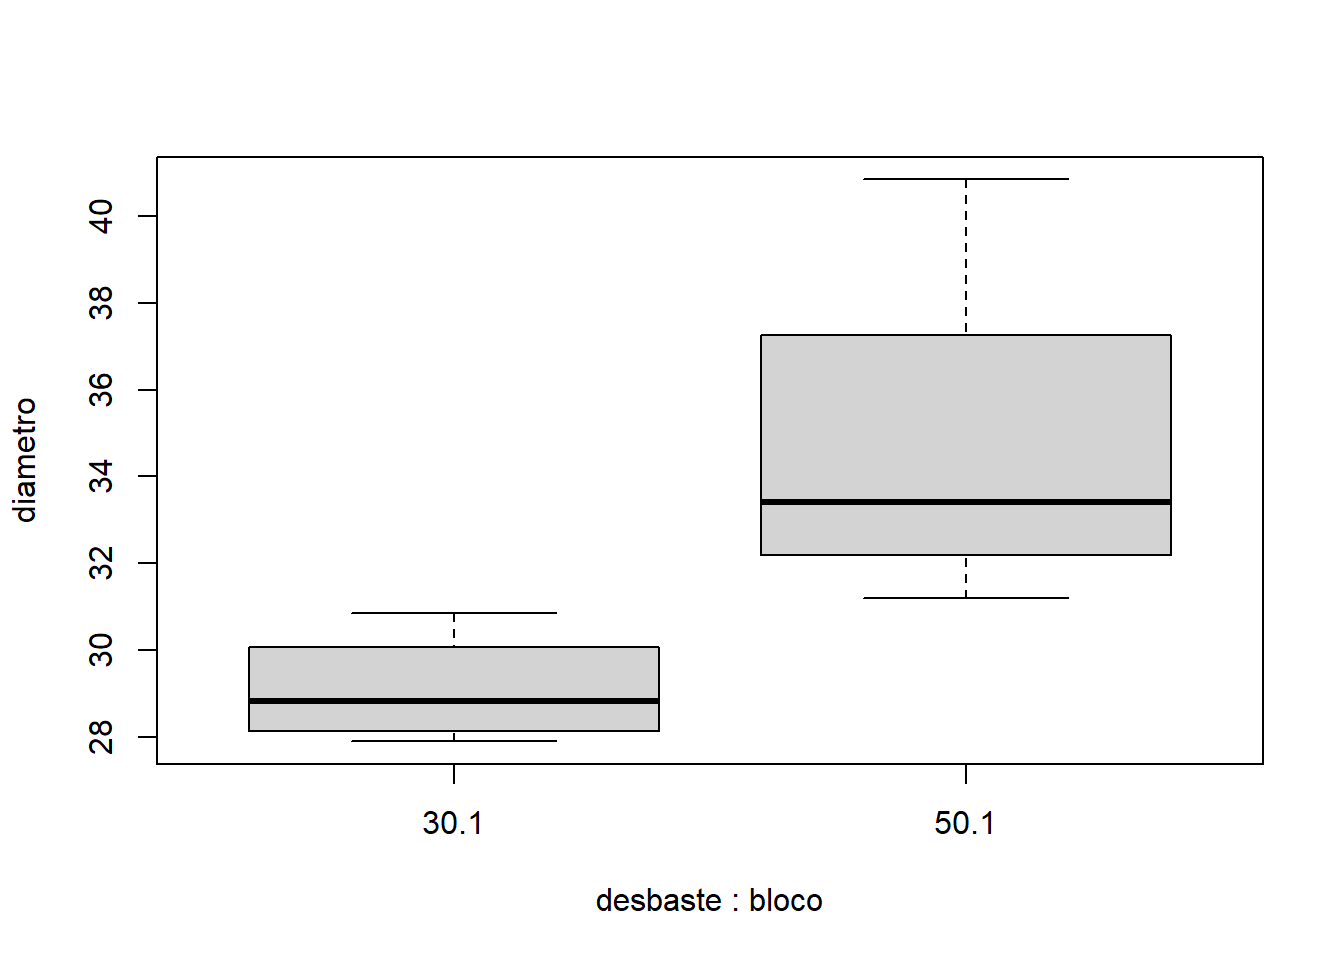
\includegraphics{bookdown_files/unnamed-chunk-69-1.png}

Pelo gráfico obtido, é razoável esperar que haja diferenças significativas entre as intensidades de desbaste (30\% e 50\%), pois existe um distanciamento entre os interquartis especialmente nos blocos 1 e 2. Também é possível esperar que não haja um efeito significativo dos blocos. Assim, espera-se que a análise estatística do experimento corrobore a conclusão empírica baseada no interpretação do gráfico.

Com a função \texttt{dbc()} do pacote \texttt{ExpDes.pt} será possível realizar toda a análise de um experimento de delineamento casualizado em blocos, inclusive desdobramentos. Para consultar a sintaxe do comando digita-se no console:

\begin{Shaded}
\begin{Highlighting}[]
\NormalTok{?dbc}
\end{Highlighting}
\end{Shaded}

Nas informações sobre a função \texttt{?dbc}, nota-se que a sintaxe básica da função \texttt{dbc()} é:

\begin{Shaded}
\begin{Highlighting}[]
\KeywordTok{dbc}\NormalTok{(trat, bloco, resp, }\DataTypeTok{quali =} \OtherTok{TRUE}\NormalTok{, }\DataTypeTok{mcomp =} \StringTok{"tukey"}\NormalTok{, }
    \DataTypeTok{sigT =} \FloatTok{0.05}\NormalTok{, }\DataTypeTok{sigF =} \FloatTok{0.05}\NormalTok{)}
\end{Highlighting}
\end{Shaded}

A análise do experimento em questão pode ser então realizada pelo comando:

\begin{Shaded}
\begin{Highlighting}[]
\KeywordTok{require}\NormalTok{(ExpDes.pt)}
\KeywordTok{dbc}\NormalTok{(dbc1}\OperatorTok{$}\NormalTok{desbaste, dbc1}\OperatorTok{$}\NormalTok{bloco, dbc1}\OperatorTok{$}\NormalTok{diametro, }\DataTypeTok{hvar=}\StringTok{'han'}\NormalTok{)}
\end{Highlighting}
\end{Shaded}

\begin{verbatim}
## ------------------------------------------------------------------------
## Quadro da analise de variancia
## ------------------------------------------------------------------------
##            GL     SQ     QM      Fc    Pr>Fc
## Tratamento  1 323.34 323.34 30.4546 0.000004
## Bloco       4  69.49  17.37  1.6363 0.187727
## Residuo    34 360.98  10.62                 
## Total      39 753.80                        
## ------------------------------------------------------------------------
## CV = 11.09 %
## 
## ------------------------------------------------------------------------
## Teste de normalidade dos residuos 
## valor-p:  0.9155415 
## De acordo com o teste de Shapiro-Wilk a 5% de significancia, os residuos podem ser considerados normais.
## ------------------------------------------------------------------------
## 
## ------------------------------------------------------------------------
## Teste de homogeneidade de variancia 
## valor-p:  0.3001718 
## De acordo com o teste de han a 5% de significancia, as variancias podem ser consideradas homogeneas.
## ------------------------------------------------------------------------
## 
## Teste de Tukey
## ------------------------------------------------------------------------
## Grupos Tratamentos Medias
## a     50      32.21285 
##  b    30      26.52659 
## ------------------------------------------------------------------------
\end{verbatim}

A interpretação da saída de um delineamento casualizado em blocos é muito parecido com os experimento em DIC. A inclusão do bloco como fonte de variação, não trás nenhuma implicação já que o bloco visa apenas isolar um potencial efeito do ambiente não controlado durante a instalação do experimento.

Neste primeiro exemplo, os resíduos apresentaram normalidade e homogeneidade de variâncias. Note que o teste apresentado para avaliar a homogeneidade de variâncias é diferente do que foi utilizado para o DIC. No caso do DIC foi realizado o teste de bartlett que não é aconselhado para aplicar em DBC em razão das variâncias não serem independentes entre si. No DBC foi apresentado o teste de Han, que é um teste considerado mais adquedo para delineamentos em blocos.

O efeito do tratamento foi significativo. Como existem apenas dois níveis, a significância do teste F já é conclusivo. Neste caso indicando que há diferença entre tratamentos. Neste caso não haveria a necessidade de aplicar um teste de média, mas a saída do teste de média já é padrão do pacote \texttt{ExpDes.pt}. O teste de médias que apenas reforça o resultado do teste F, indicando que o grupo \texttt{a} obteve média maior que o grupo \texttt{b}.

\hypertarget{o-caso-desbalanceado-1}{%
\subsection{O caso desbalanceado}\label{o-caso-desbalanceado-1}}

Embora o delineamento casualizado em blocos, tenha além do tratamento, o efeito do bloco, estes são analisados de forma independente sem considerar a interação entre eles. A rigor, a definição de blocos visa apenas controlar uma possível fonte de variação do ambiente não controlada pelo experimento. Desta forma, por não haver interação, o caso de DBC desbalanceado pode ser analisado através da ANOVA do Tipo I.

Na sequência, será utilizado o mesmo exemplo anterior, mas assumindo que foi perdida uma parcela devido à um incêndio: a repetição 1, do bloco 2 do tratamento intensidade de desbaste de 30\%:

\begin{itemize}
\tightlist
\item
  Tratamento: 2 intensidades de desbaste
\item
  5 Blocos
\item
  4 repetições
\item
  Variável de interesse: diâmetro
\item
  Parcela perdida: Tratamento 30, Bloco 2, Repetição 1.
\end{itemize}

\begin{table}

\caption{\label{tab:unnamed-chunk-73}Dados de outro delineamento casualizado em blocos, porém neste caso desbalanceado.}
\centering
\begin{tabular}[t]{r|r|r|r}
\hline
desbaste & bloco & rep & diametro\\
\hline
30 & 1 & 1 & 28.37041\\
\hline
30 & 1 & 2 & 29.28010\\
\hline
30 & 1 & 3 & 30.84926\\
\hline
30 & 1 & 4 & 27.89227\\
\hline
30 & 2 & 2 & 21.47290\\
\hline
30 & 2 & 3 & 24.39744\\
\hline
30 & 2 & 4 & 24.65861\\
\hline
30 & 3 & 1 & 23.79856\\
\hline
30 & 3 & 2 & 25.69388\\
\hline
30 & 3 & 3 & 24.45922\\
\hline
30 & 3 & 4 & 27.94071\\
\hline
30 & 4 & 1 & 28.05501\\
\hline
30 & 4 & 2 & 26.42934\\
\hline
30 & 4 & 3 & 23.09124\\
\hline
30 & 4 & 4 & 22.54273\\
\hline
30 & 5 & 1 & 32.73052\\
\hline
30 & 5 & 2 & 29.17538\\
\hline
30 & 5 & 3 & 29.94747\\
\hline
30 & 5 & 4 & 29.35810\\
\hline
50 & 1 & 1 & 31.20701\\
\hline
50 & 1 & 2 & 40.85273\\
\hline
50 & 1 & 3 & 33.66891\\
\hline
50 & 1 & 4 & 33.15001\\
\hline
50 & 2 & 1 & 34.03869\\
\hline
50 & 2 & 2 & 36.24517\\
\hline
50 & 2 & 3 & 35.49081\\
\hline
50 & 2 & 4 & 31.58952\\
\hline
50 & 3 & 1 & 31.92634\\
\hline
50 & 3 & 2 & 28.82107\\
\hline
50 & 3 & 3 & 32.18963\\
\hline
50 & 3 & 4 & 31.55686\\
\hline
50 & 4 & 1 & 31.11534\\
\hline
50 & 4 & 2 & 31.05093\\
\hline
50 & 4 & 3 & 34.69215\\
\hline
50 & 4 & 4 & 32.95378\\
\hline
50 & 5 & 1 & 25.26880\\
\hline
50 & 5 & 2 & 30.48375\\
\hline
50 & 5 & 3 & 31.73922\\
\hline
50 & 5 & 4 & 26.21619\\
\hline
\end{tabular}
\end{table}

O primeiro passo é importar o arquivo csv contendo os resultados do experimento para dentro do R. Esta tarefa pode ser realizada através do seguinte comando:

\begin{Shaded}
\begin{Highlighting}[]
\NormalTok{dbc2 =}\StringTok{ }\KeywordTok{read.csv}\NormalTok{(}\StringTok{"./data/Experimento DBC 2.csv"}\NormalTok{)}
\end{Highlighting}
\end{Shaded}

Mesmo no caso desbalanceado, a análise gráfica é fundamental e deve preceder qualquer análise estatística:

\begin{Shaded}
\begin{Highlighting}[]
\KeywordTok{boxplot}\NormalTok{(}\DataTypeTok{data =}\NormalTok{ dbc2, diametro }\OperatorTok{~}\StringTok{ }\NormalTok{desbaste}\OperatorTok{/}\NormalTok{bloco)}
\end{Highlighting}
\end{Shaded}

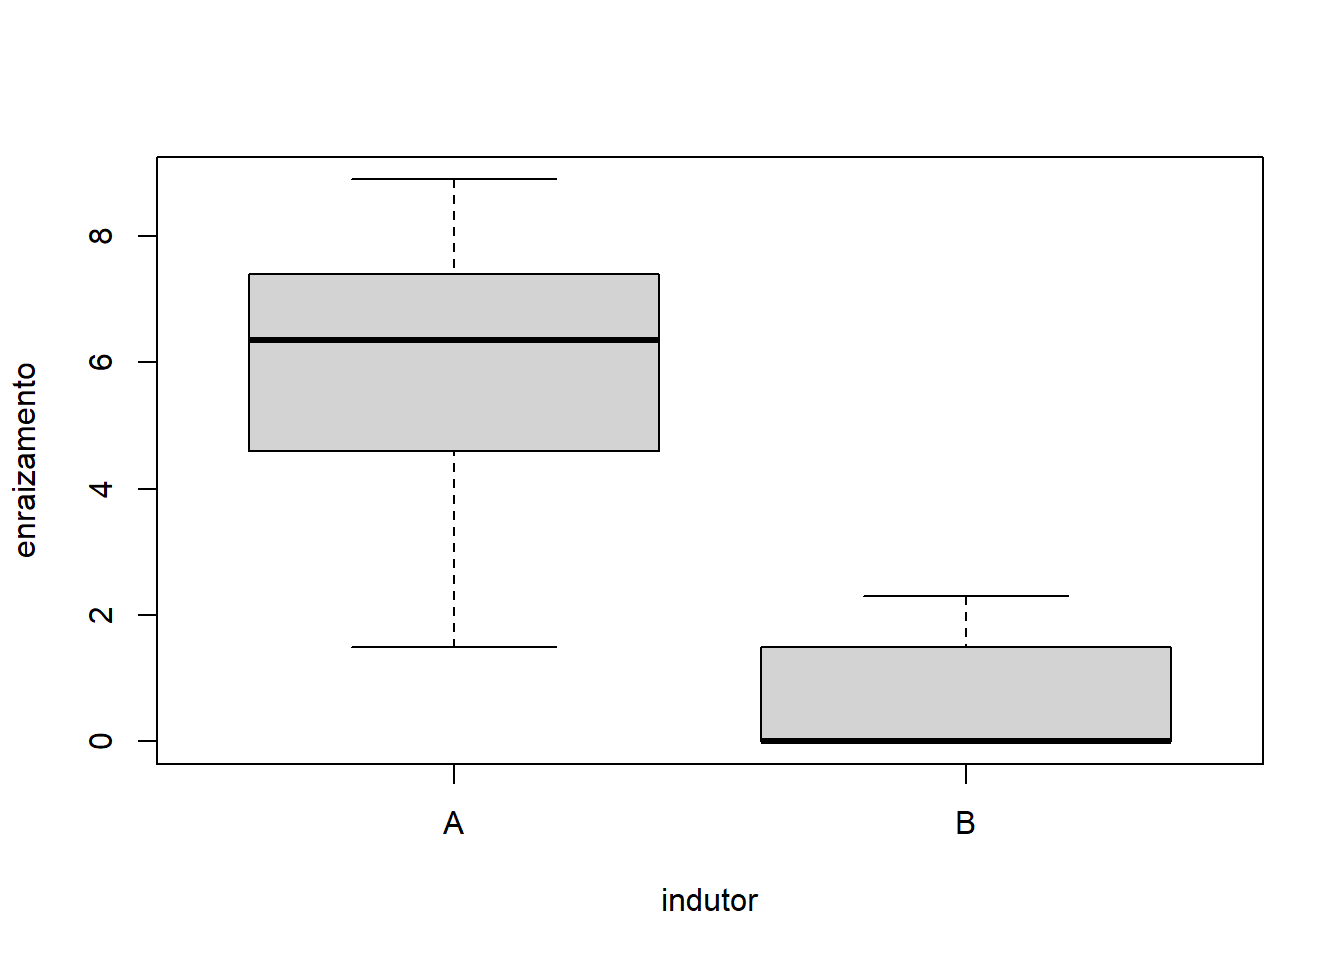
\includegraphics{bookdown_files/unnamed-chunk-75-1.png}

Os tratamentos podem ser analisados isoladamente em relação a cada bloco, utilizando um filtro para escolher qual bloco considerar.

\begin{enumerate}
\def\labelenumi{\arabic{enumi}.}
\tightlist
\item
  Para bloco igual a 1:
\end{enumerate}

\begin{Shaded}
\begin{Highlighting}[]
\KeywordTok{boxplot}\NormalTok{(}\DataTypeTok{data =}\NormalTok{ dbc2[dbc2}\OperatorTok{$}\NormalTok{bloco }\OperatorTok{==}\StringTok{ }\DecValTok{1}\NormalTok{,], diametro}\OperatorTok{~}\NormalTok{desbaste}\OperatorTok{/}\NormalTok{bloco)}
\end{Highlighting}
\end{Shaded}

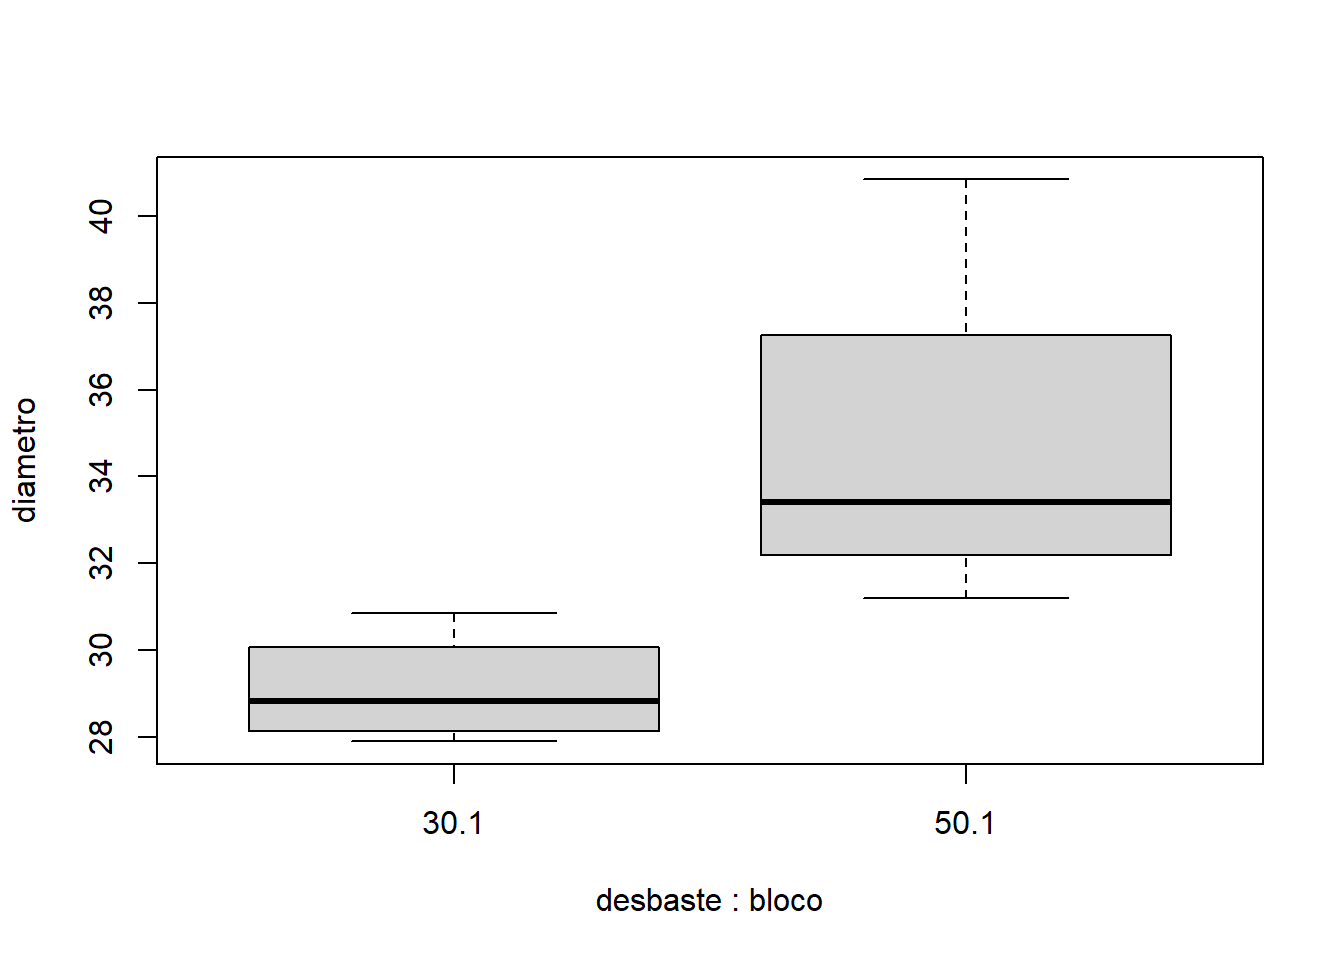
\includegraphics{bookdown_files/unnamed-chunk-76-1.png}

\begin{enumerate}
\def\labelenumi{\arabic{enumi}.}
\setcounter{enumi}{1}
\tightlist
\item
  Para bloco igual a 2:
\end{enumerate}

\begin{Shaded}
\begin{Highlighting}[]
\KeywordTok{boxplot}\NormalTok{(}\DataTypeTok{data =}\NormalTok{ dbc2[dbc2}\OperatorTok{$}\NormalTok{bloco }\OperatorTok{==}\StringTok{ }\DecValTok{2}\NormalTok{,], diametro}\OperatorTok{~}\NormalTok{desbaste}\OperatorTok{/}\NormalTok{bloco)}
\end{Highlighting}
\end{Shaded}

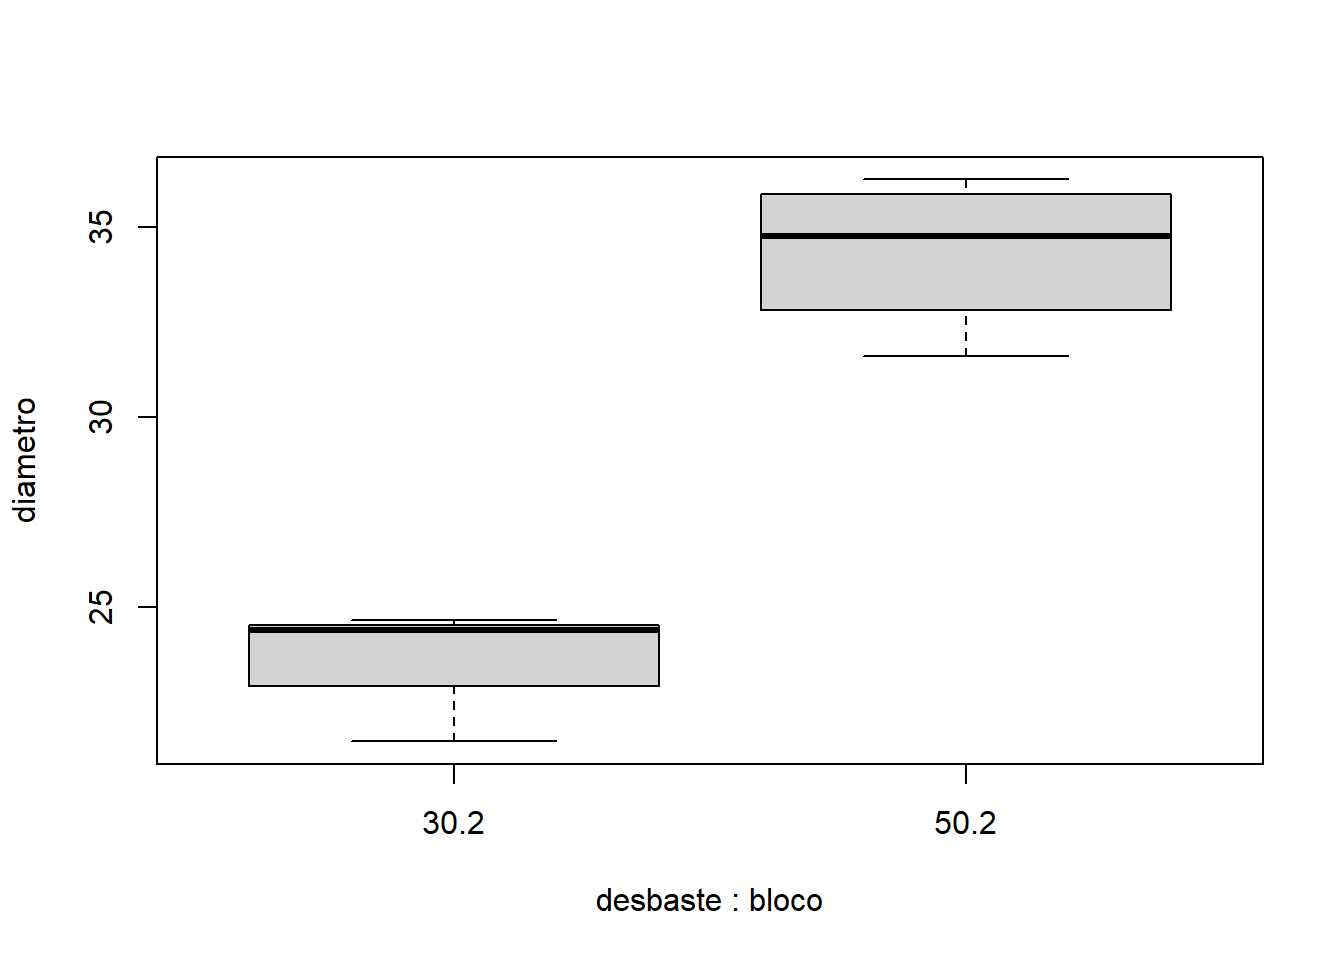
\includegraphics{bookdown_files/unnamed-chunk-77-1.png}

\begin{enumerate}
\def\labelenumi{\arabic{enumi}.}
\setcounter{enumi}{2}
\tightlist
\item
  Para bloco igual a 3:
\end{enumerate}

\begin{Shaded}
\begin{Highlighting}[]
\KeywordTok{boxplot}\NormalTok{(}\DataTypeTok{data =}\NormalTok{ dbc2[dbc2}\OperatorTok{$}\NormalTok{bloco }\OperatorTok{==}\StringTok{ }\DecValTok{3}\NormalTok{,], diametro}\OperatorTok{~}\NormalTok{desbaste}\OperatorTok{/}\NormalTok{bloco)}
\end{Highlighting}
\end{Shaded}

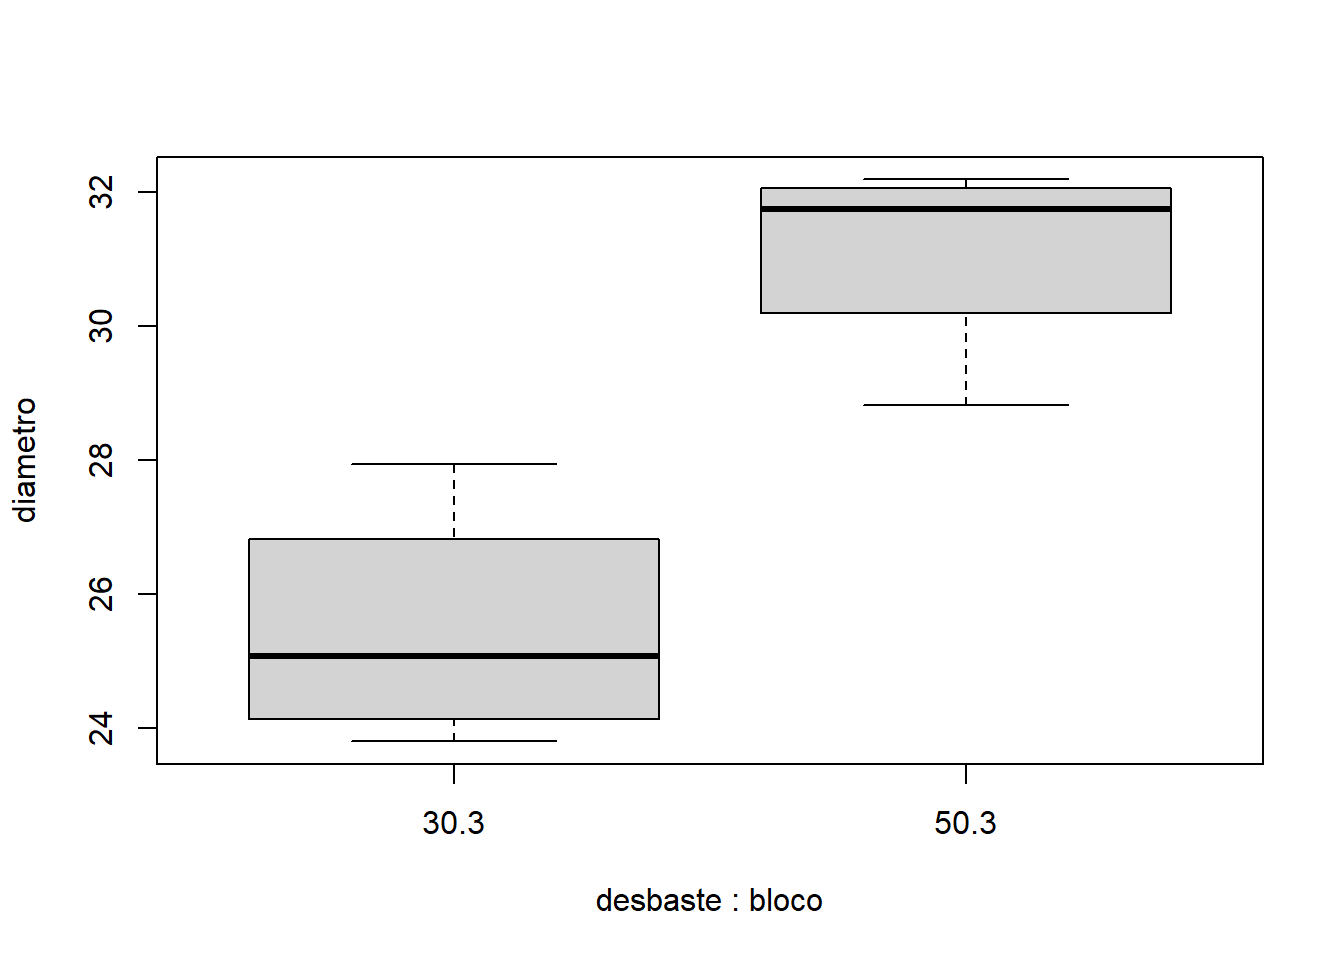
\includegraphics{bookdown_files/unnamed-chunk-78-1.png}

\begin{enumerate}
\def\labelenumi{\arabic{enumi}.}
\setcounter{enumi}{3}
\tightlist
\item
  Para bloco igual a 4:
\end{enumerate}

\begin{Shaded}
\begin{Highlighting}[]
\KeywordTok{boxplot}\NormalTok{(}\DataTypeTok{data =}\NormalTok{ dbc2[dbc2}\OperatorTok{$}\NormalTok{bloco }\OperatorTok{==}\StringTok{ }\DecValTok{4}\NormalTok{,], diametro}\OperatorTok{~}\NormalTok{desbaste}\OperatorTok{/}\NormalTok{bloco)}
\end{Highlighting}
\end{Shaded}

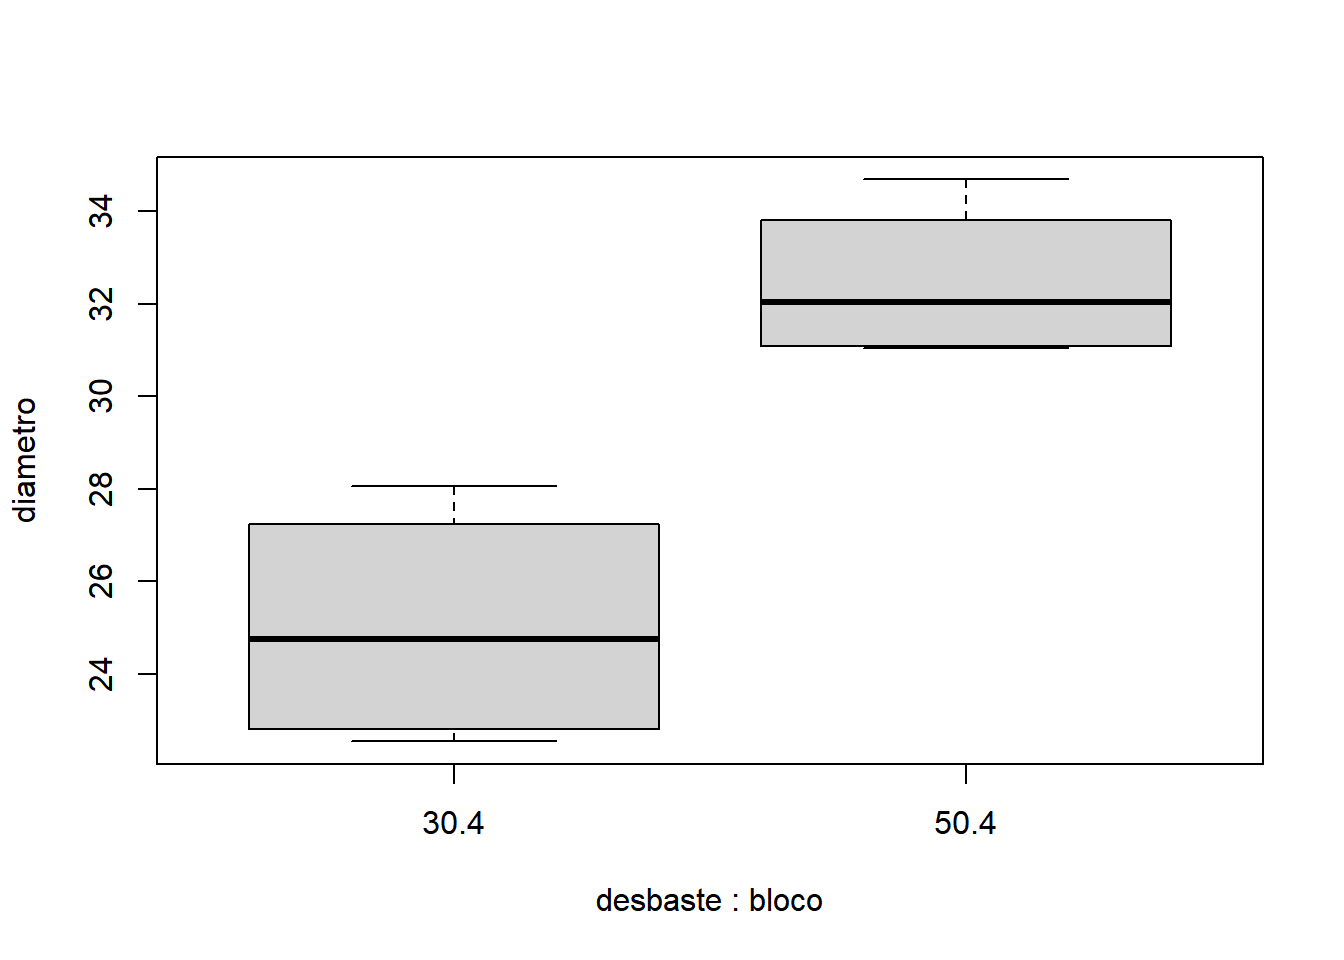
\includegraphics{bookdown_files/unnamed-chunk-79-1.png}

\begin{enumerate}
\def\labelenumi{\arabic{enumi}.}
\setcounter{enumi}{4}
\tightlist
\item
  Para bloco igual a 5:
\end{enumerate}

\begin{Shaded}
\begin{Highlighting}[]
\KeywordTok{boxplot}\NormalTok{(}\DataTypeTok{data =}\NormalTok{ dbc2[dbc2}\OperatorTok{$}\NormalTok{bloco }\OperatorTok{==}\StringTok{ }\DecValTok{5}\NormalTok{,], diametro}\OperatorTok{~}\NormalTok{desbaste}\OperatorTok{/}\NormalTok{bloco)}
\end{Highlighting}
\end{Shaded}

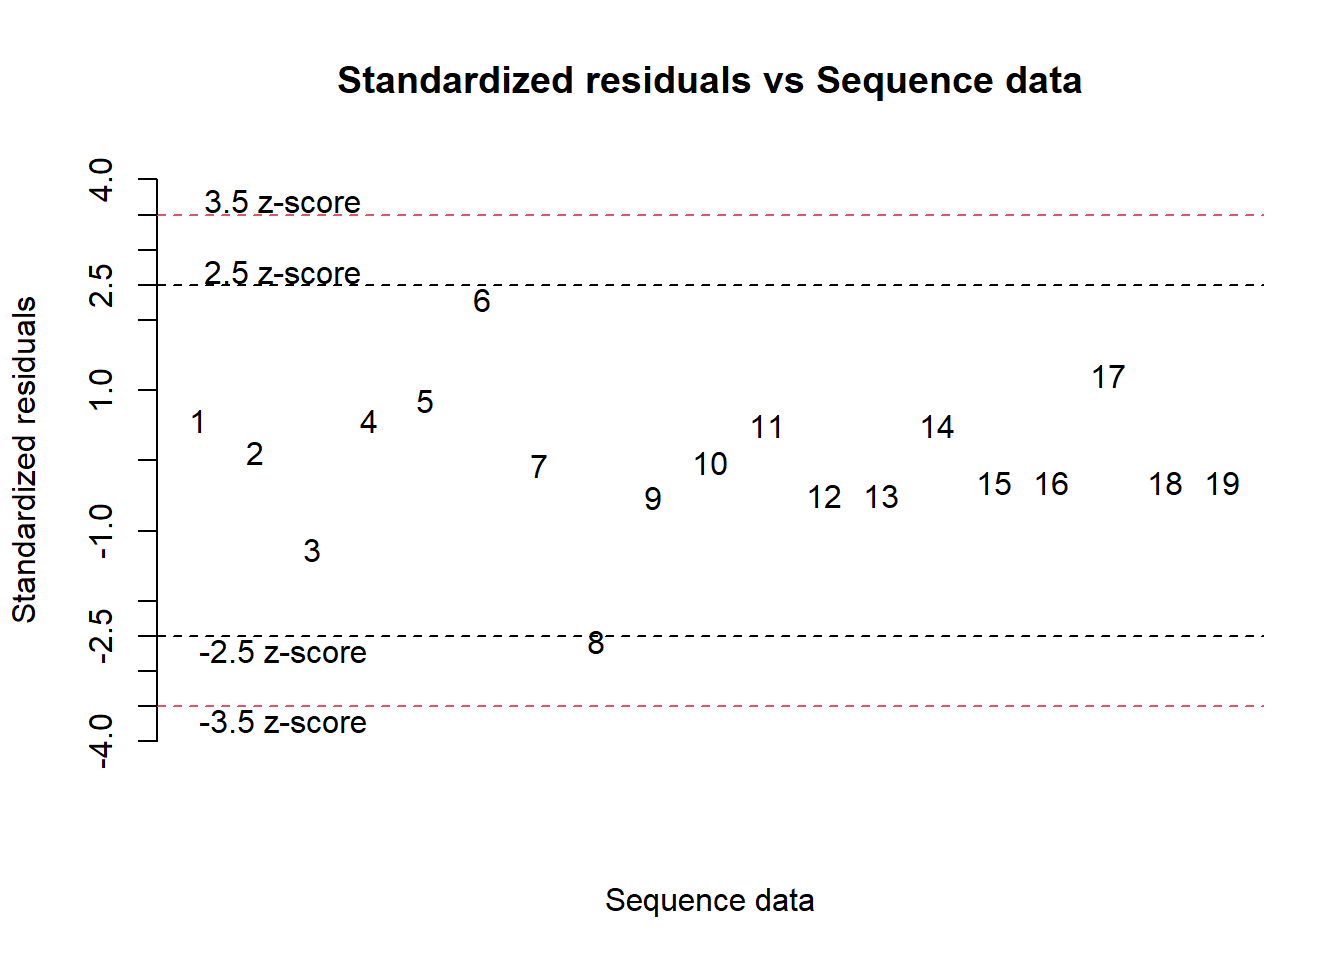
\includegraphics{bookdown_files/unnamed-chunk-80-1.png}

Como já discutido anteriormente, por não haver cálculo de interação entre fontes de variação, o DBC pode ser analisado usando o pacote \texttt{ExpDes.pt} e sua função \texttt{dbc()}:

\begin{Shaded}
\begin{Highlighting}[]
\KeywordTok{require}\NormalTok{(ExpDes.pt)}
\KeywordTok{dbc}\NormalTok{(dbc2}\OperatorTok{$}\NormalTok{desbaste, dbc2}\OperatorTok{$}\NormalTok{bloco, dbc2}\OperatorTok{$}\NormalTok{diametro, }\DataTypeTok{hvar=}\StringTok{'han'}\NormalTok{)}
\end{Highlighting}
\end{Shaded}

\begin{verbatim}
## ------------------------------------------------------------------------
## Quadro da analise de variancia
## ------------------------------------------------------------------------
##            GL     SQ      QM      Fc    Pr>Fc
## Tratamento  1 280.26 280.264 28.2071 0.000007
## Bloco       4  62.92  15.731  1.5832 0.201872
## Residuo    33 327.89   9.936                 
## Total      38 671.07                         
## ------------------------------------------------------------------------
## CV = 10.65 %
## 
## ------------------------------------------------------------------------
## Teste de normalidade dos residuos 
## valor-p:  0.9523324 
## De acordo com o teste de Shapiro-Wilk a 5% de significancia, os residuos podem ser considerados normais.
## ------------------------------------------------------------------------
## 
## ------------------------------------------------------------------------
## Teste de homogeneidade de variancia 
## valor-p:  0.3579419 
## De acordo com o teste de han a 5% de significancia, as variancias podem ser consideradas homogeneas.
## ------------------------------------------------------------------------
## 
## Teste de Tukey
## ------------------------------------------------------------------------
## Grupos Tratamentos Medias
## a     50      32.21285 
##  b    30      26.84964 
## ------------------------------------------------------------------------
\end{verbatim}

\hypertarget{fatorial-duplo-inteiramento-casualizado}{%
\section{Fatorial duplo inteiramento casualizado}\label{fatorial-duplo-inteiramento-casualizado}}

No caso de um fatorial inteiramente casualizado, a ANOVA contará com quatro fontes de variação: uma fonte de variação conhecida determinada pelo tratamento A, outra fonte de variação conhecida determinada pelo tratamento B, outra fonte de variação conhecida determinada pela interação entre os dois tratamentos e uma quarta fonte de variação desconhecida determinada pelo resíduo. O modelo estatístico do delineamento fatorial duplo inteiramente casualizado é:

\[Y = \bar{Y} + TRAT_A + TRAT_B + (TRAT_A * TRAT_B) + Erro\]

A análise começa pela determinação das somas de quadrados total, composta pela soma de quadrados do fator 1, pela soma de quadrados do fator 2, pela soma de quadrados da interação dos dois fatores e pela soma de quadrados do resíduo. Em seguida, calculam-se os quadrados médios do fator 1, fator 2, interação e do resíduo. A estatística F será computada para cada um dos fatores, bem como sua interação. Se F calculado for superior ao F tabelado, assume-se que existe um efeito devido ao respectivo fator (ou interação), ao passo que se F calculado for inferior ao F tabelado, não há evidências suficientes para rejeitar a hipótese nula, aceitando-se a hipótese de que não existe efeito do fator (ou da interação). Sendo a interação significativa, parte-se direto para o desdobramento de um fator dentro do outro. Apenas no caso de interação não significativa, considera-se o desdobramento dos fatores isolados.

\hypertarget{o-caso-balanceado-2}{%
\subsection{O caso balanceado}\label{o-caso-balanceado-2}}

Neste exemplo de delineamento inteiramente casualizado em esquema fatorial observa-se um experimento que avaliou o efeito de dois indutores de enraizamento em duas concentrações no enraizamento de estacas de uma espécie de árvore nativa do cerrado brasileiro. Os dados podem ser resumidos através dos seguintes tópicos:

\begin{itemize}
\tightlist
\item
  Fator 1: indutor A e indutor B
\item
  Fator 2: Dose 10 e 20\%
\item
  5 repetições
\item
  Variável de interesse: número médio de raízes
\end{itemize}

\begin{table}

\caption{\label{tab:unnamed-chunk-82}Dados de experimento em fatorial em DIC}
\centering
\begin{tabular}[t]{l|r|r|r}
\hline
indutor & concentracao & rep & enraizamento\\
\hline
A & 10 & 1 & 7.4\\
\hline
A & 10 & 2 & 6.7\\
\hline
A & 10 & 3 & 4.6\\
\hline
A & 10 & 4 & 7.4\\
\hline
A & 10 & 5 & 6.0\\
\hline
A & 20 & 1 & 6.7\\
\hline
A & 20 & 2 & 8.9\\
\hline
A & 20 & 3 & 5.3\\
\hline
A & 20 & 4 & 1.5\\
\hline
A & 20 & 5 & 4.6\\
\hline
B & 10 & 1 & 0.7\\
\hline
B & 10 & 2 & 1.5\\
\hline
B & 10 & 3 & 0.0\\
\hline
B & 10 & 4 & 0.0\\
\hline
B & 10 & 5 & 1.5\\
\hline
B & 20 & 1 & 0.0\\
\hline
B & 20 & 2 & 0.0\\
\hline
B & 20 & 3 & 2.3\\
\hline
B & 20 & 4 & 0.0\\
\hline
B & 20 & 5 & 0.0\\
\hline
\end{tabular}
\end{table}

O primeiro passo é importar o arquivo contendo os resultados do experimento para dentro do R. Esta tarefa pode ser realizada através do seguinte comando:

\begin{Shaded}
\begin{Highlighting}[]
\NormalTok{fatDIC1 =}\StringTok{ }\KeywordTok{read.csv}\NormalTok{(}\StringTok{"./data/Experimento Fatorial Duplo DIC 1.csv"}\NormalTok{)}
\end{Highlighting}
\end{Shaded}

Antes da análise estatística, exploram-se os dados através dos gráficos \texttt{boxplot()} ou \texttt{plot()}. Com base nos dados do experimento em questão, vamos analisá-lo através de uma série de gráficos boxplot. Embora a concentração seja uma variável contínua, este fator possui apenas dois níveis e portanto não é suficiente para considerar uma análise de tendência utilizando regressão.

\begin{enumerate}
\def\labelenumi{\arabic{enumi}.}
\tightlist
\item
  Considerando apenas fator 1:
\end{enumerate}

\begin{Shaded}
\begin{Highlighting}[]
\KeywordTok{boxplot}\NormalTok{(}\DataTypeTok{data =}\NormalTok{ fatDIC1, enraizamento }\OperatorTok{~}\StringTok{ }\NormalTok{indutor)}
\end{Highlighting}
\end{Shaded}

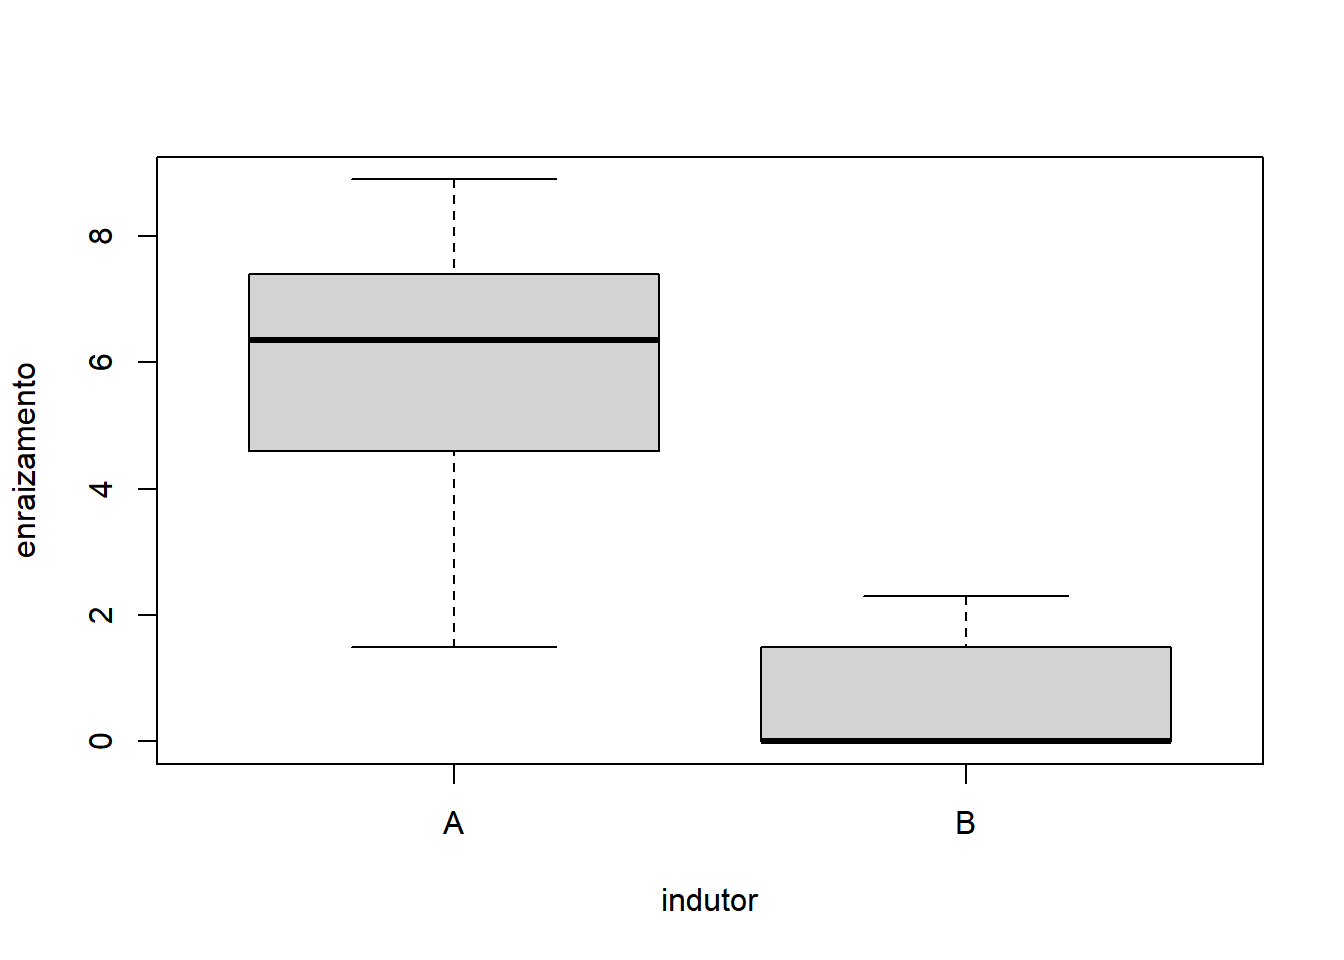
\includegraphics{bookdown_files/unnamed-chunk-84-1.png}

\begin{enumerate}
\def\labelenumi{\arabic{enumi}.}
\setcounter{enumi}{1}
\tightlist
\item
  Considerando apenas fator 2:
\end{enumerate}

\begin{Shaded}
\begin{Highlighting}[]
\KeywordTok{boxplot}\NormalTok{(}\DataTypeTok{data =}\NormalTok{ fatDIC1, enraizamento }\OperatorTok{~}\StringTok{ }\NormalTok{concentracao)}
\end{Highlighting}
\end{Shaded}

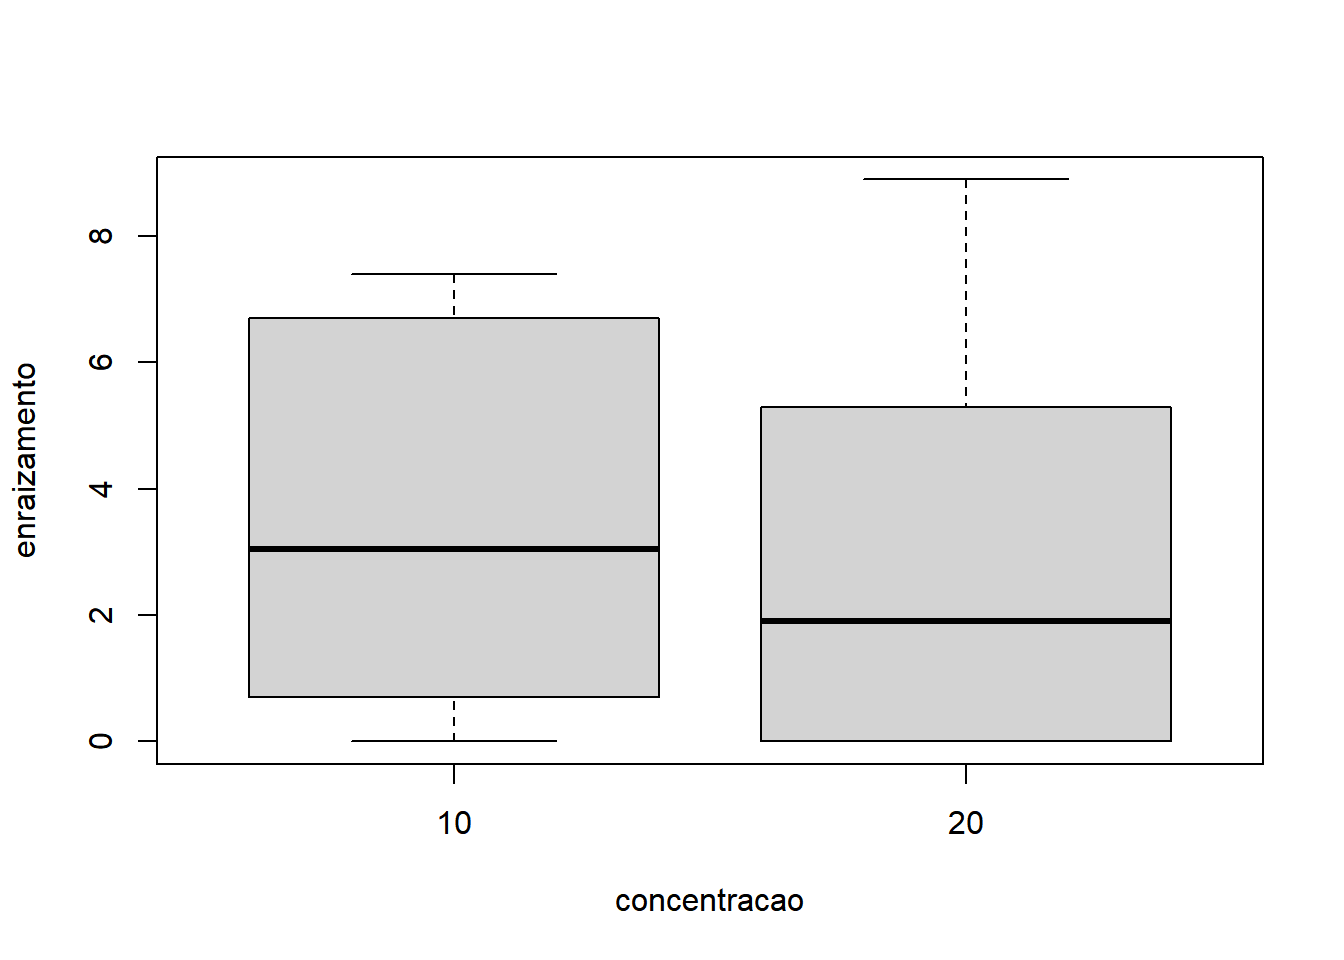
\includegraphics{bookdown_files/unnamed-chunk-85-1.png}

\begin{enumerate}
\def\labelenumi{\arabic{enumi}.}
\setcounter{enumi}{2}
\tightlist
\item
  Interação dos fatores:
\end{enumerate}

\begin{Shaded}
\begin{Highlighting}[]
\KeywordTok{boxplot}\NormalTok{(}\DataTypeTok{data =}\NormalTok{ fatDIC1, enraizamento }\OperatorTok{~}\StringTok{ }\NormalTok{indutor}\OperatorTok{/}\NormalTok{concentracao)}
\end{Highlighting}
\end{Shaded}

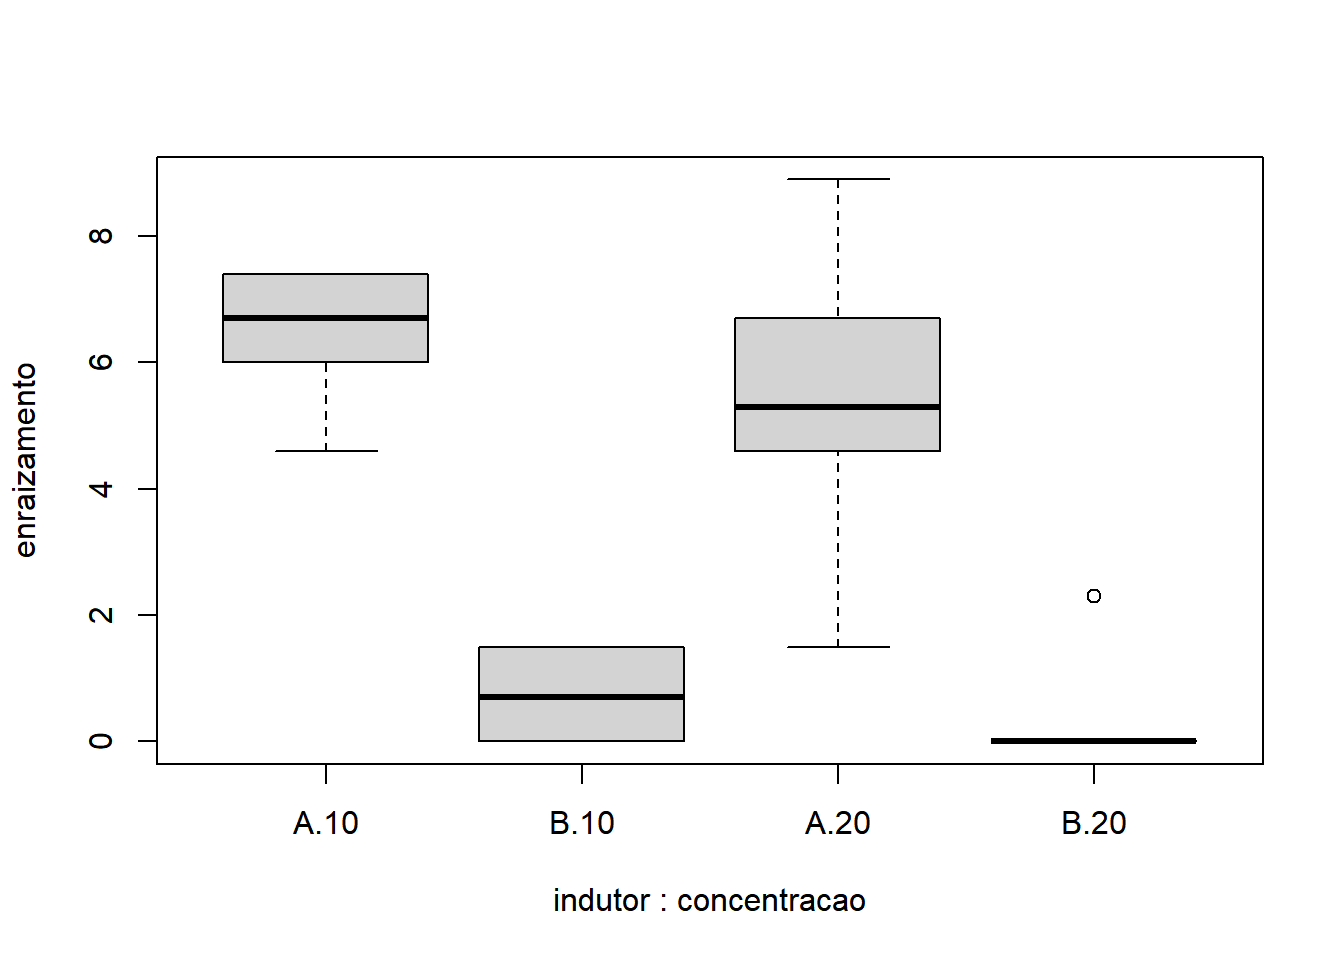
\includegraphics{bookdown_files/unnamed-chunk-86-1.png}

\begin{enumerate}
\def\labelenumi{\arabic{enumi}.}
\setcounter{enumi}{3}
\tightlist
\item
  Fixando concentracao igual a 10:
\end{enumerate}

\begin{Shaded}
\begin{Highlighting}[]
\KeywordTok{boxplot}\NormalTok{(}\DataTypeTok{data =}\NormalTok{ fatDIC1[fatDIC1}\OperatorTok{$}\NormalTok{concentracao }\OperatorTok{==}\StringTok{ }\DecValTok{10}\NormalTok{,], }
\NormalTok{        enraizamento }\OperatorTok{~}\StringTok{ }\NormalTok{indutor)}
\end{Highlighting}
\end{Shaded}

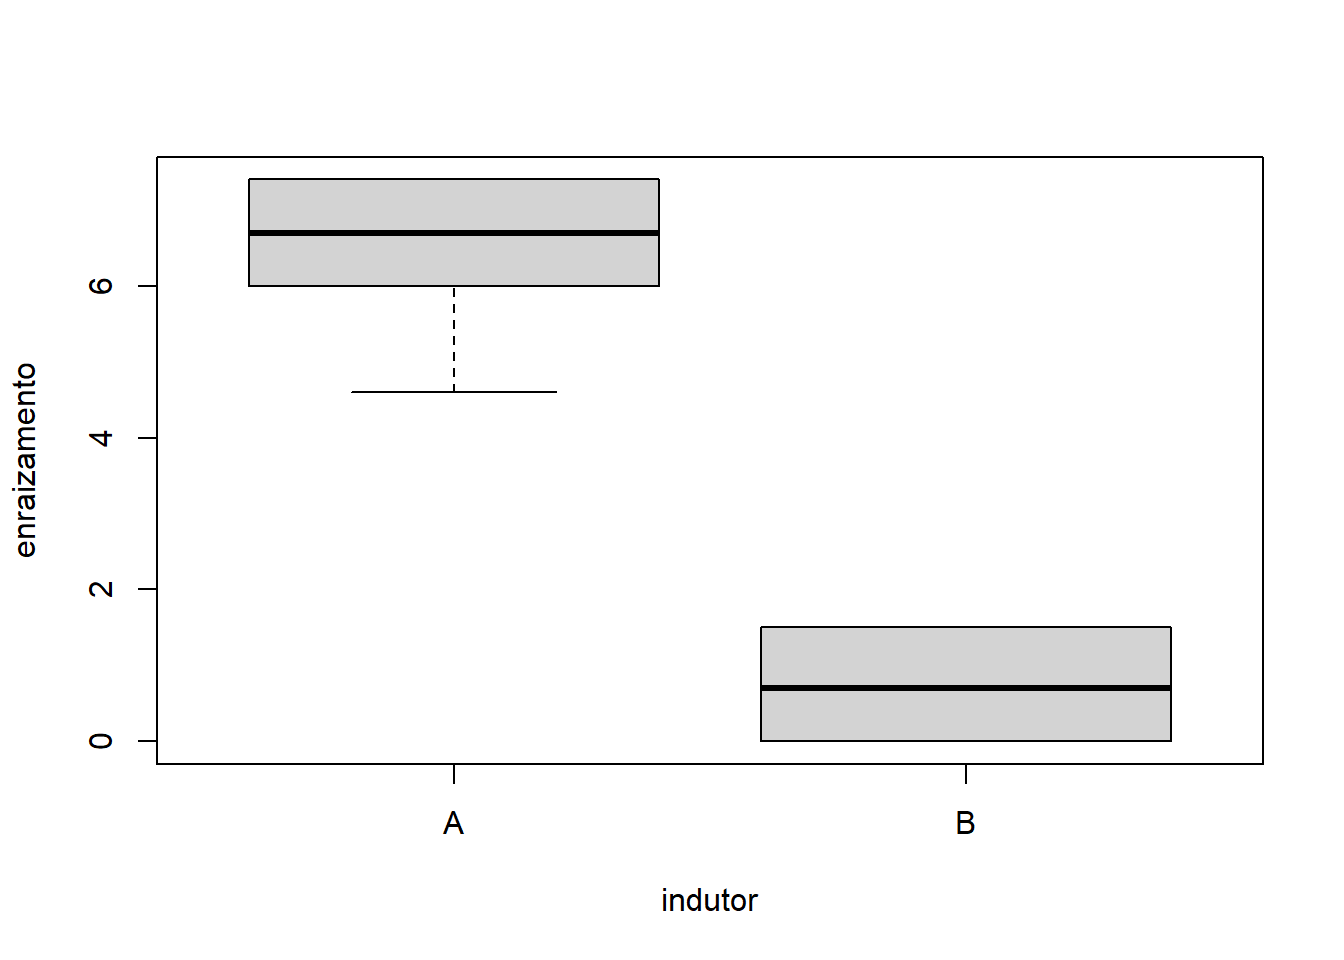
\includegraphics{bookdown_files/unnamed-chunk-87-1.png}

\begin{enumerate}
\def\labelenumi{\arabic{enumi}.}
\setcounter{enumi}{4}
\tightlist
\item
  Fixando concentracao igual a 20:
\end{enumerate}

\begin{Shaded}
\begin{Highlighting}[]
\KeywordTok{boxplot}\NormalTok{(}\DataTypeTok{data =}\NormalTok{ fatDIC1[fatDIC1}\OperatorTok{$}\NormalTok{concentracao }\OperatorTok{==}\StringTok{ }\DecValTok{20}\NormalTok{,], }
\NormalTok{        enraizamento }\OperatorTok{~}\StringTok{ }\NormalTok{indutor)}
\end{Highlighting}
\end{Shaded}

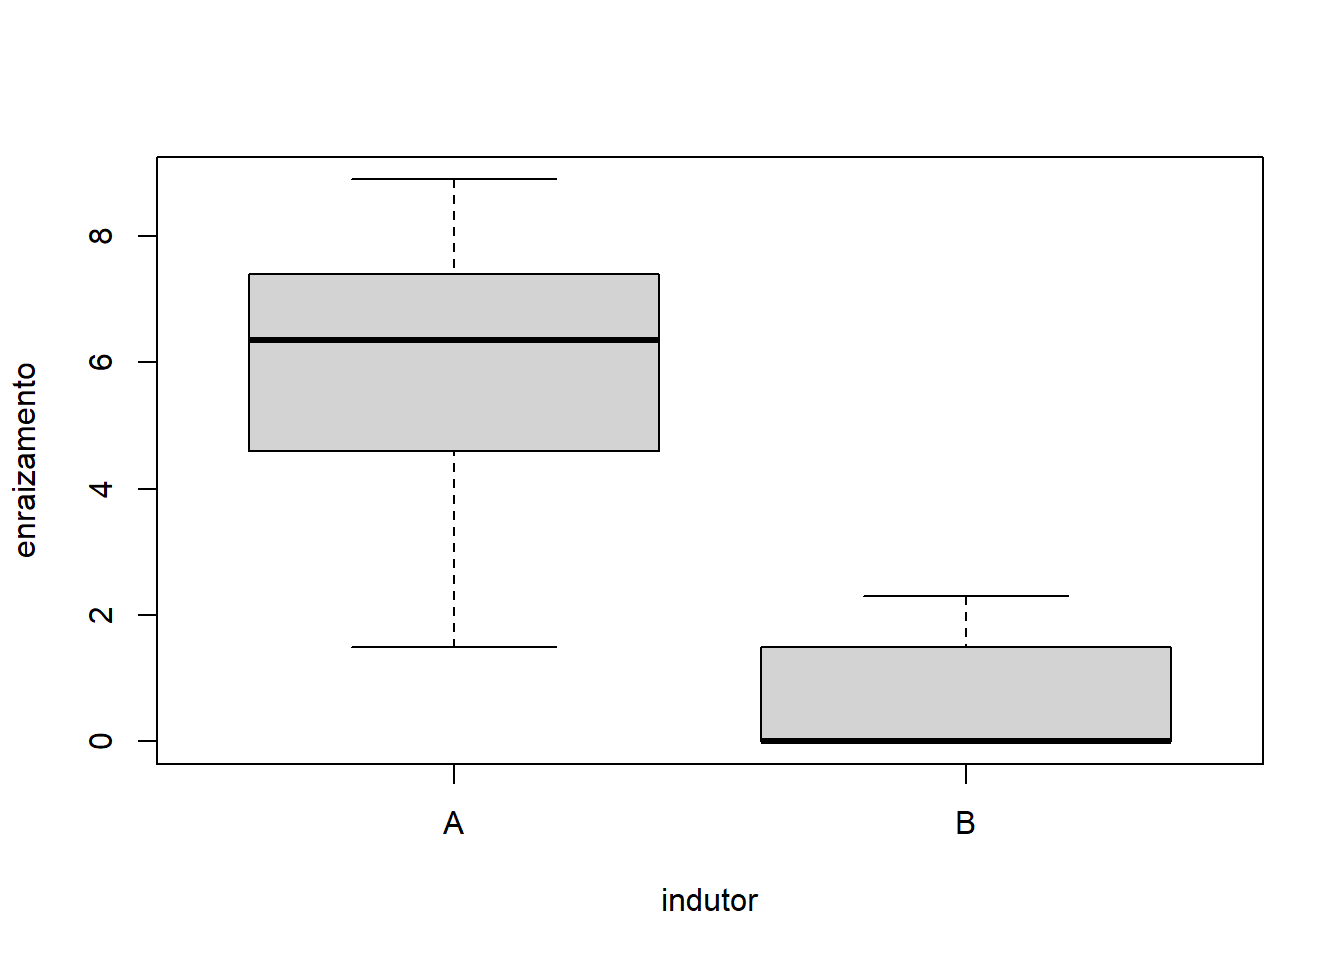
\includegraphics{bookdown_files/unnamed-chunk-88-1.png}

\begin{enumerate}
\def\labelenumi{\arabic{enumi}.}
\setcounter{enumi}{5}
\tightlist
\item
  Fixando Indutor igual a `A':
\end{enumerate}

\begin{Shaded}
\begin{Highlighting}[]
\KeywordTok{boxplot}\NormalTok{(}\DataTypeTok{data =}\NormalTok{ fatDIC1[fatDIC1}\OperatorTok{$}\NormalTok{indutor }\OperatorTok{==}\StringTok{ "A"}\NormalTok{,], }
\NormalTok{        enraizamento }\OperatorTok{~}\StringTok{ }\NormalTok{concentracao)}
\end{Highlighting}
\end{Shaded}

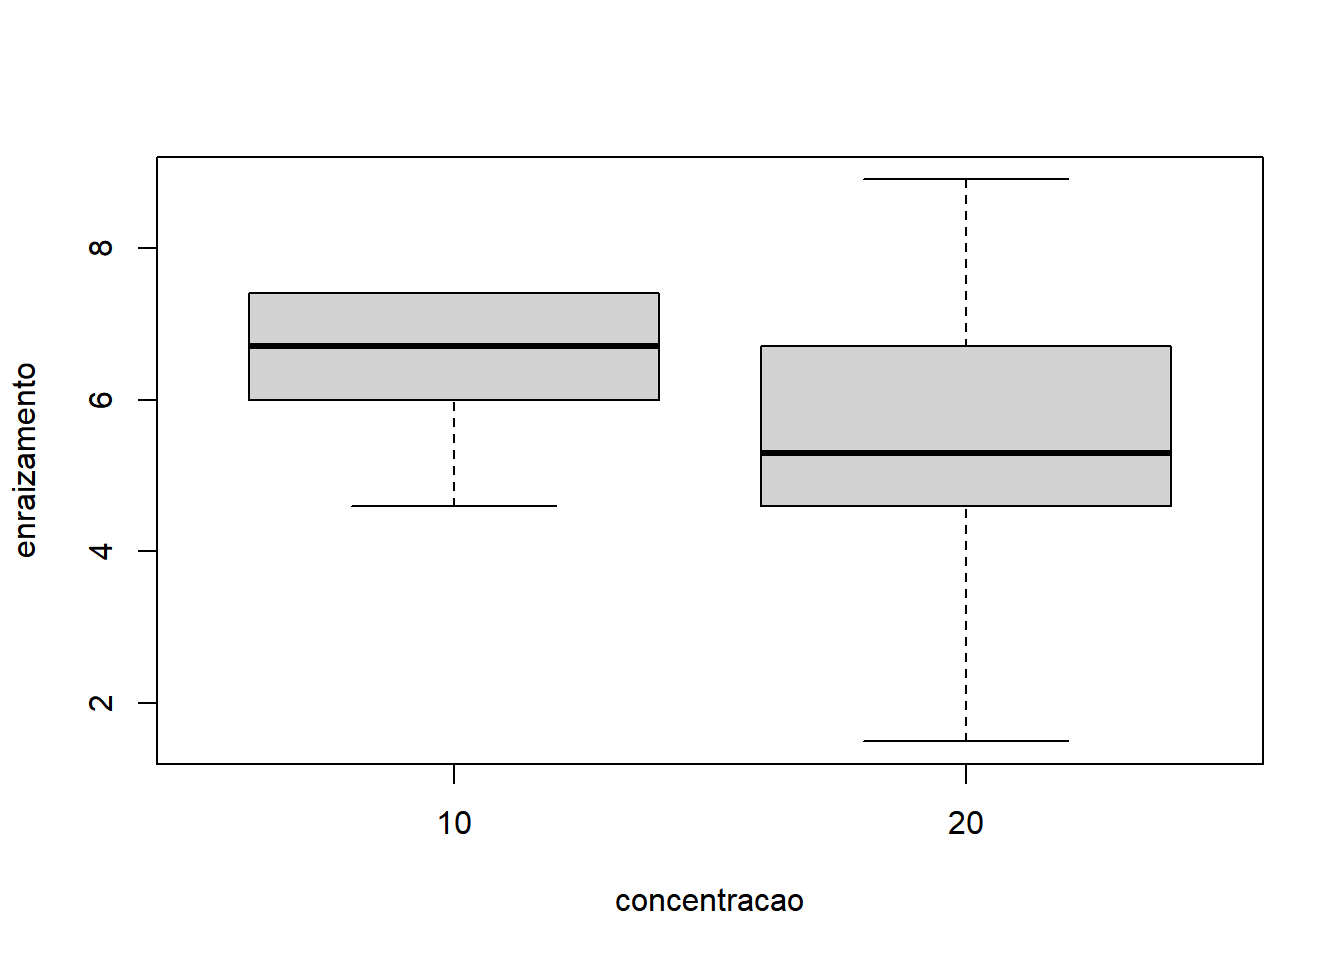
\includegraphics{bookdown_files/unnamed-chunk-89-1.png}

\begin{enumerate}
\def\labelenumi{\arabic{enumi}.}
\setcounter{enumi}{6}
\tightlist
\item
  Fixando Indutor igual a `B':
\end{enumerate}

\begin{Shaded}
\begin{Highlighting}[]
\KeywordTok{boxplot}\NormalTok{(}\DataTypeTok{data =}\NormalTok{ fatDIC1[fatDIC1}\OperatorTok{$}\NormalTok{indutor }\OperatorTok{==}\StringTok{ "B"}\NormalTok{,], }
\NormalTok{        enraizamento }\OperatorTok{~}\StringTok{ }\NormalTok{concentracao)}
\end{Highlighting}
\end{Shaded}

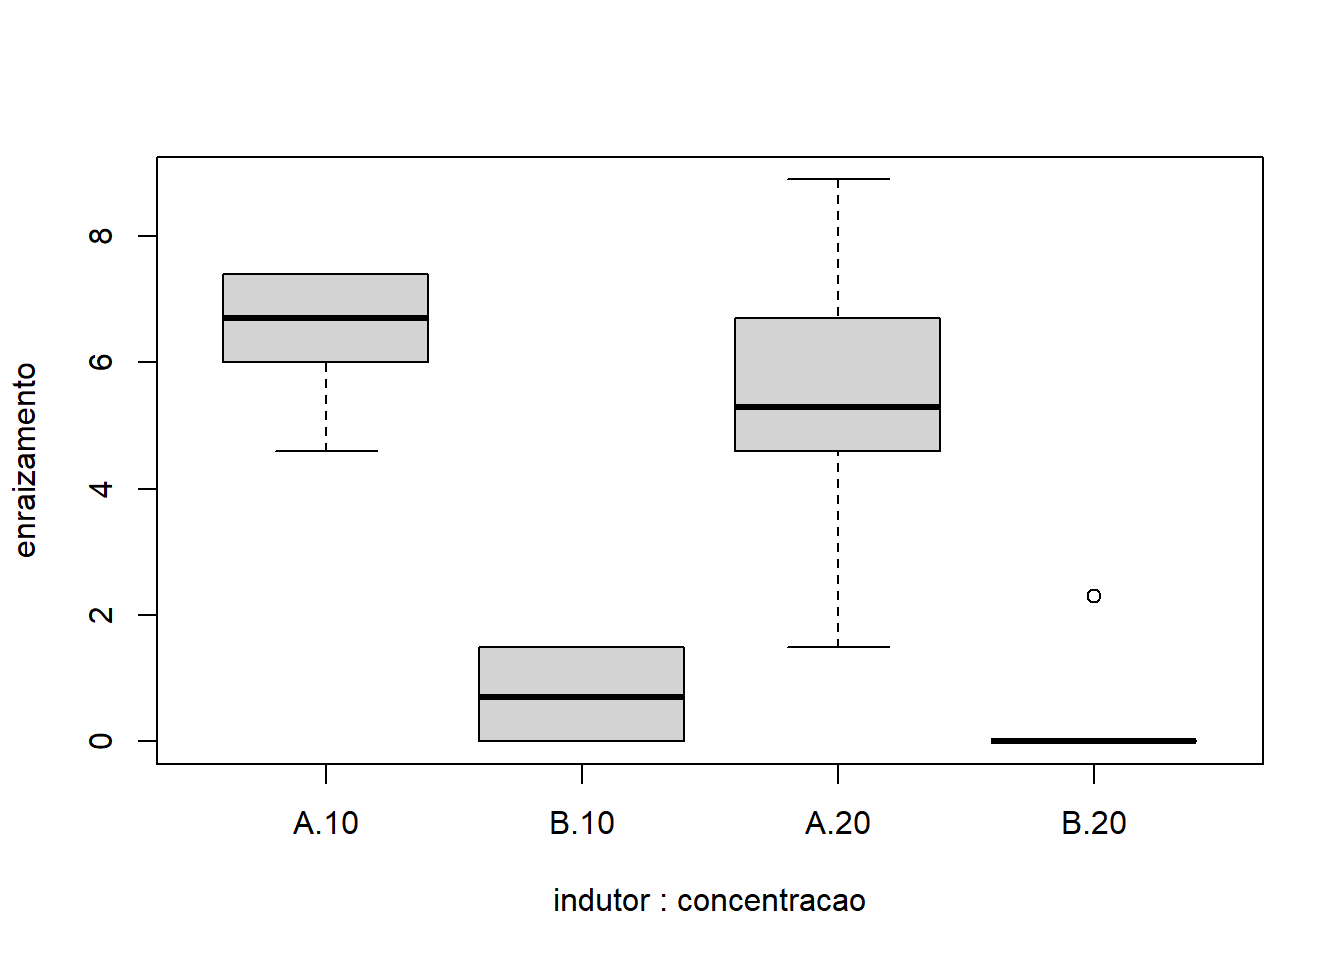
\includegraphics{bookdown_files/unnamed-chunk-90-1.png}

Com base nos gráficos, é razoável apontar que o fator Indutor apresentou maior variação do que o fator Concentração. A interação também não parece influenciar o comportamento já identificado pelos fatores, quando analisados isoladamente.

A função do pacote \texttt{ExpDes.pt} para análise deste tipo de experimento é a \texttt{fat2.dic()}. A sintaxe desta função é:

\begin{Shaded}
\begin{Highlighting}[]
\KeywordTok{fat2.dic}\NormalTok{(fator1, fator2, resp, }\DataTypeTok{quali =} \KeywordTok{c}\NormalTok{(}\OtherTok{TRUE}\NormalTok{, }\OtherTok{TRUE}\NormalTok{), }
         \DataTypeTok{mcomp =} \StringTok{"tukey"}\NormalTok{, }\DataTypeTok{fac.names =} \KeywordTok{c}\NormalTok{(}\StringTok{"F1"}\NormalTok{, }\StringTok{"F2"}\NormalTok{), }
         \DataTypeTok{sigT =} \FloatTok{0.05}\NormalTok{, }\DataTypeTok{sigF =} \FloatTok{0.05}\NormalTok{)}
\end{Highlighting}
\end{Shaded}

Ajustando com base nos dados do experimento, o comando fica:

\begin{Shaded}
\begin{Highlighting}[]
\KeywordTok{require}\NormalTok{(ExpDes.pt)}
\KeywordTok{fat2.dic}\NormalTok{(fatDIC1}\OperatorTok{$}\NormalTok{indutor, fatDIC1}\OperatorTok{$}\NormalTok{concentracao,                        }
\NormalTok{         fatDIC1}\OperatorTok{$}\NormalTok{enraizamento, }\DataTypeTok{quali =} \KeywordTok{c}\NormalTok{(}\OtherTok{TRUE}\NormalTok{, }\OtherTok{TRUE}\NormalTok{),}
         \DataTypeTok{fac.names =} \KeywordTok{c}\NormalTok{(}\StringTok{"Indutor"}\NormalTok{, }\StringTok{"Concentração"}\NormalTok{))}
\end{Highlighting}
\end{Shaded}

\begin{verbatim}
## ------------------------------------------------------------------------
## Legenda:
## FATOR 1:  Indutor 
## FATOR 2:  Concentração 
## ------------------------------------------------------------------------
## 
## 
## Quadro da analise de variancia
## ------------------------------------------------------------------------
##                      GL      SQ      QM     Fc
## Indutor               1 140.981 140.981 54.000
## Concentração          1   2.113   2.113  0.809
## Indutor*Concentração  1   0.684   0.684  0.262
## Residuo              16  41.772   2.611       
## Total                19 185.550               
##                        Pr>Fc
## Indutor              0.00000
## Concentração         0.38171
## Indutor*Concentração 0.61562
## Residuo                     
## Total                       
## ------------------------------------------------------------------------
## CV = 49.64 %
## 
## ------------------------------------------------------------------------
## Teste de normalidade dos residuos (Shapiro-Wilk)
## valor-p:  0.144 
## De acordo com o teste de Shapiro-Wilk a 5% de significancia, os residuos podem ser considerados normais.
## ------------------------------------------------------------------------
## 
## Interacao nao significativa: analisando os efeitos simples
## ------------------------------------------------------------------------
## Indutor
## Teste de Tukey
## ------------------------------------------------------------------------
## Grupos Tratamentos Medias
## a     A   5.91 
##  b    B   0.6 
## ------------------------------------------------------------------------
## 
## Concentração
## De acordo com o teste F, as medias desse fator sao estatisticamente iguais.
## ------------------------------------------------------------------------
##   Niveis Medias
## 1     10   3.58
## 2     20   2.93
## ------------------------------------------------------------------------
\end{verbatim}

O teste Shapiro-Wilk indica que os resíduos podem ser considerados normais. Assim, o modelo estatístico é adequado e os demais resultados podem ser considerados e analisados. A interação foi não significativa, e portanto os fatores devem ser analisados de forma independente. Apenas o fator Indutor foi significativo, levando então a um desdobramento dos níveis, que indica uma média do Indutor A superior à média do Indutor B.

\hypertarget{o-caso-desbalanceado-2}{%
\subsection{O caso desbalanceado}\label{o-caso-desbalanceado-2}}

Neste exemplo de delineamento inteiramente casualizado em esquema fatorial, com dados desbalanceados, tem-se um experimento para avaliar o enraizamento de dois tipos de substratos e duas intensidades de irrigação. Infelizmente, uma das bandejas de enraizamento foi contaminada com fungo e portanto foi considerada perdida. Por isto, este é um exemplo de experimento desbalanceado. Os dados podem ser resumidos através dos seguintes tópicos:

\begin{itemize}
\tightlist
\item
  Fator 1: substrato A e B
\item
  Fator 2: intensidade de irrigação 10 mm e 20 mm
\item
  5 repetições
\item
  Informação perdida: Repetição 5 do substrato A, intensidade de irrigação 10 mm
\item
  Variável de interesse: número médio de raízes
\end{itemize}

\begin{table}

\caption{\label{tab:unnamed-chunk-93}Dados de experimento em fatorial em DIC, porém desbalanceado.}
\centering
\begin{tabular}[t]{l|r|r|r}
\hline
substrato & irrigacao & rep & enraizamento\\
\hline
A & 10 & 1 & 7.4\\
\hline
A & 10 & 2 & 6.7\\
\hline
A & 10 & 3 & 4.6\\
\hline
A & 10 & 4 & 7.4\\
\hline
A & 20 & 1 & 6.7\\
\hline
A & 20 & 2 & 8.9\\
\hline
A & 20 & 3 & 5.3\\
\hline
A & 20 & 4 & 1.5\\
\hline
A & 20 & 5 & 4.6\\
\hline
B & 10 & 1 & 0.7\\
\hline
B & 10 & 2 & 1.5\\
\hline
B & 10 & 3 & 0.0\\
\hline
B & 10 & 4 & 0.0\\
\hline
B & 10 & 5 & 1.5\\
\hline
B & 20 & 1 & 0.0\\
\hline
B & 20 & 2 & 0.0\\
\hline
B & 20 & 3 & 2.3\\
\hline
B & 20 & 4 & 0.0\\
\hline
B & 20 & 5 & 0.0\\
\hline
\end{tabular}
\end{table}

O primeiro passo é importar o arquivo contendo os resultados do experimento para dentro do R. Esta tarefa pode ser realizada através do seguinte comando:

\begin{Shaded}
\begin{Highlighting}[]
\NormalTok{fatDIC2 =}\StringTok{ }\KeywordTok{read.csv}\NormalTok{(}\StringTok{"./data/Experimento Fatorial Duplo DIC 2.csv"}\NormalTok{, }
                   \DataTypeTok{sep =} \StringTok{","}\NormalTok{, }\DataTypeTok{dec =} \StringTok{"."}\NormalTok{)}
\end{Highlighting}
\end{Shaded}

Assim como no caso balanceado, é fundamental analisar os dados do experimento em gráficos e buscar antecipar os resultados que serão obtidos no teste estatístico. Os mesmo gráficos do exemplo balanceado podem ser utilizados:

\begin{enumerate}
\def\labelenumi{\arabic{enumi}.}
\tightlist
\item
  Considerando apenas fator 1:
\end{enumerate}

\begin{Shaded}
\begin{Highlighting}[]
\KeywordTok{boxplot}\NormalTok{(}\DataTypeTok{data =}\NormalTok{ fatDIC2, enraizamento }\OperatorTok{~}\StringTok{ }\NormalTok{substrato)}
\end{Highlighting}
\end{Shaded}

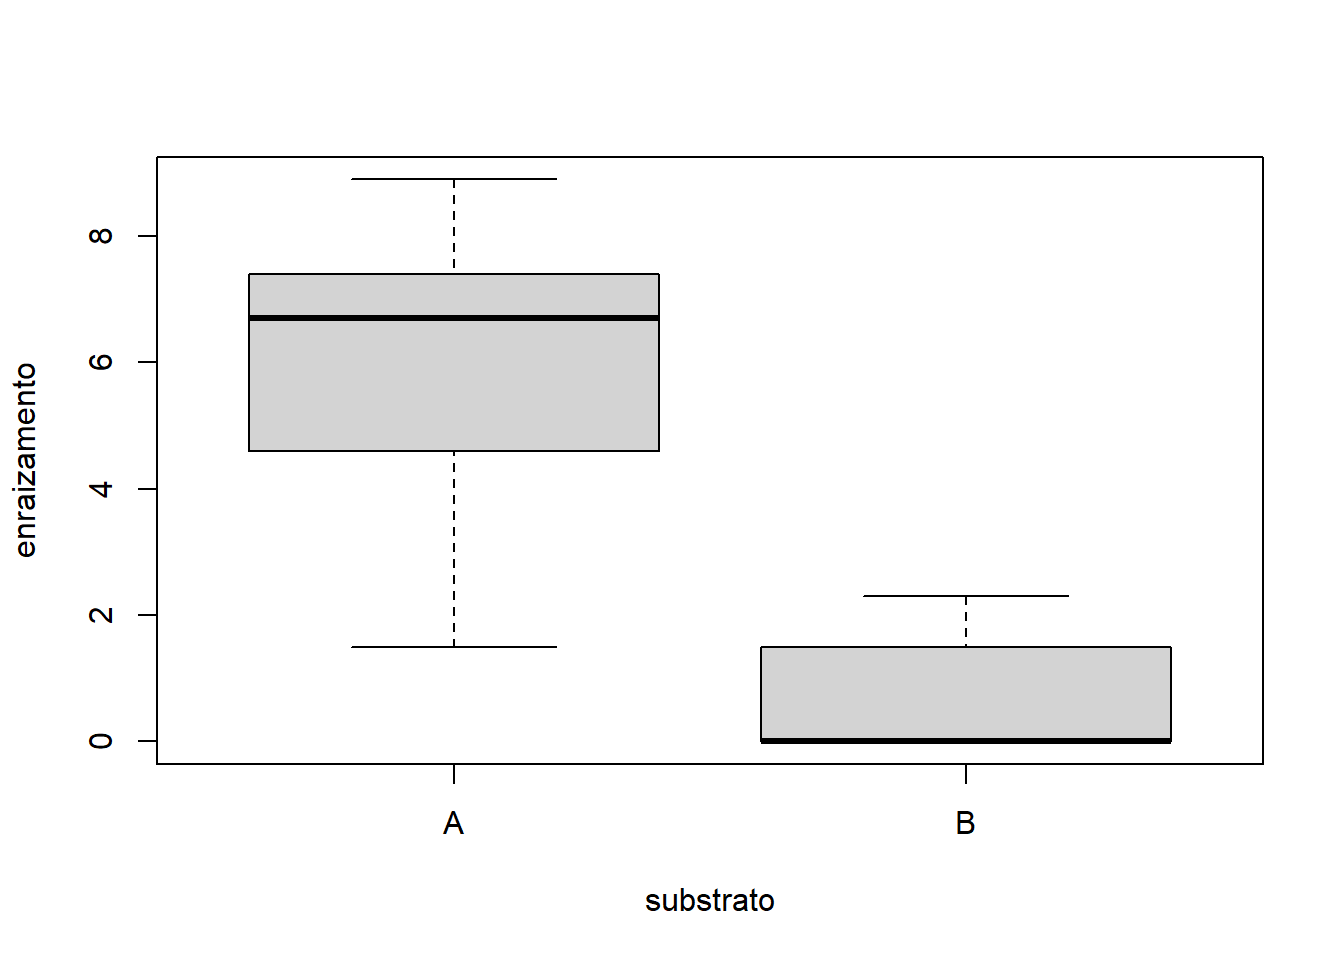
\includegraphics{bookdown_files/unnamed-chunk-95-1.png}

\begin{enumerate}
\def\labelenumi{\arabic{enumi}.}
\setcounter{enumi}{1}
\tightlist
\item
  Considerando apenas fator 2:
\end{enumerate}

\begin{Shaded}
\begin{Highlighting}[]
\KeywordTok{boxplot}\NormalTok{(}\DataTypeTok{data =}\NormalTok{ fatDIC2, enraizamento }\OperatorTok{~}\StringTok{ }\NormalTok{irrigacao)}
\end{Highlighting}
\end{Shaded}

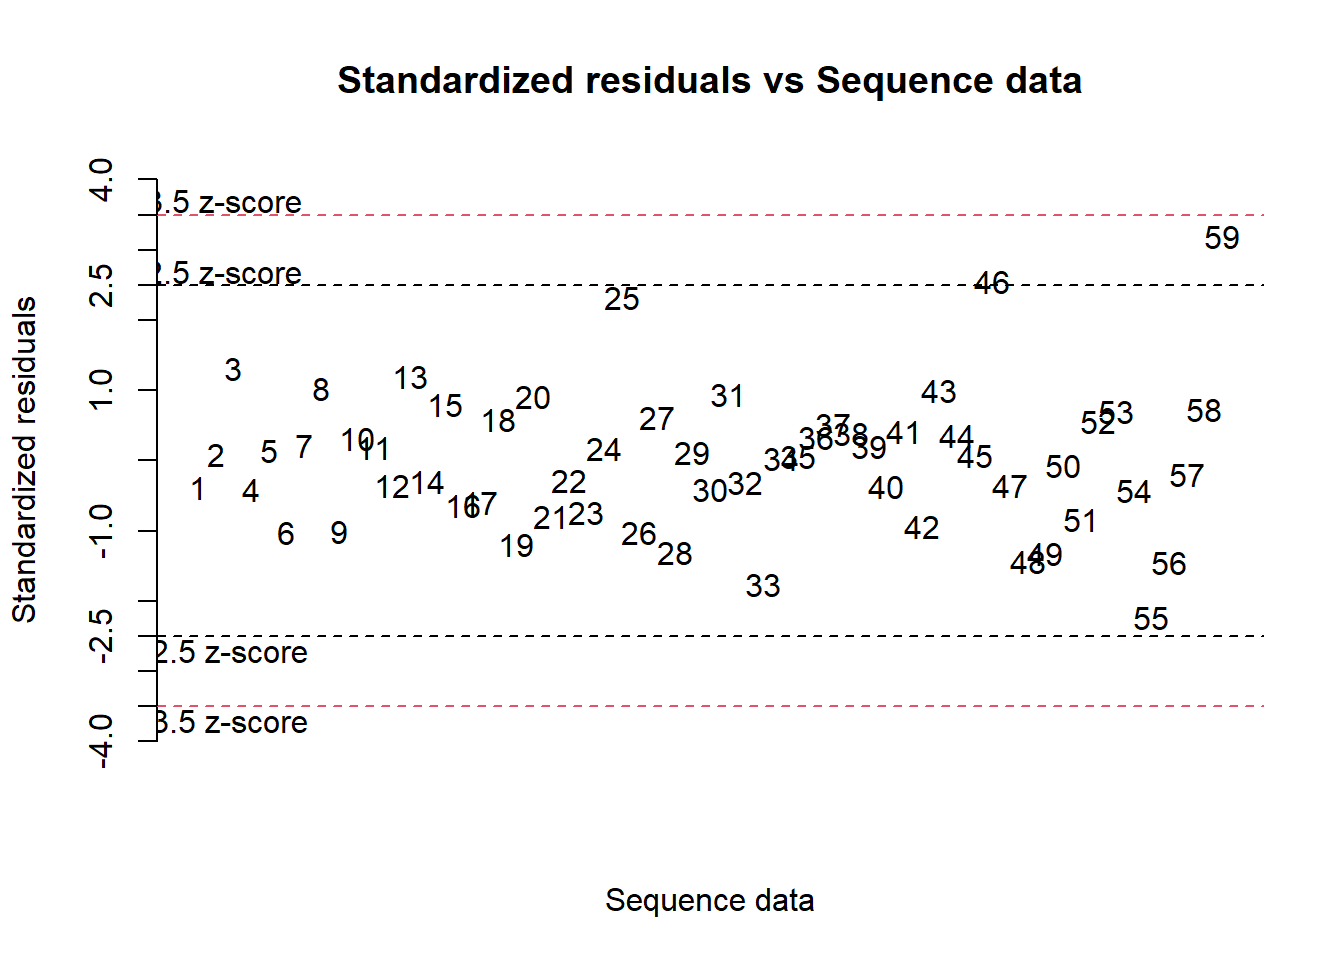
\includegraphics{bookdown_files/unnamed-chunk-96-1.png}

\begin{enumerate}
\def\labelenumi{\arabic{enumi}.}
\setcounter{enumi}{2}
\tightlist
\item
  Interação dos fatores:
\end{enumerate}

\begin{Shaded}
\begin{Highlighting}[]
\KeywordTok{boxplot}\NormalTok{(}\DataTypeTok{data =}\NormalTok{ fatDIC2, enraizamento }\OperatorTok{~}\StringTok{ }\NormalTok{substrato}\OperatorTok{/}\NormalTok{irrigacao)}
\end{Highlighting}
\end{Shaded}

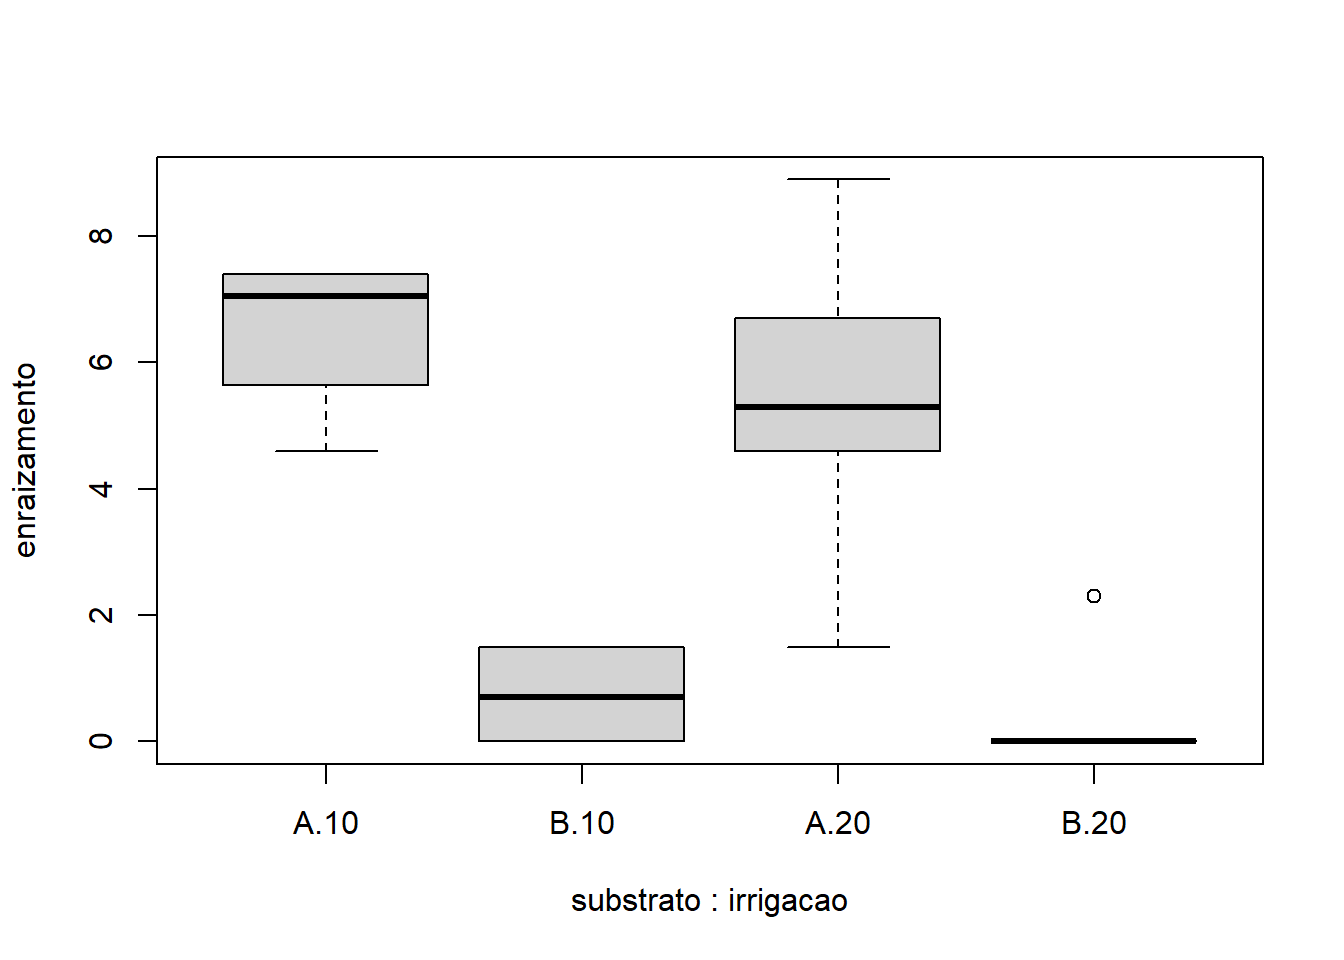
\includegraphics{bookdown_files/unnamed-chunk-97-1.png}

\begin{enumerate}
\def\labelenumi{\arabic{enumi}.}
\setcounter{enumi}{3}
\tightlist
\item
  Fixando concentracao igual a 10:
\end{enumerate}

\begin{Shaded}
\begin{Highlighting}[]
\KeywordTok{boxplot}\NormalTok{(}\DataTypeTok{data =}\NormalTok{ fatDIC2[fatDIC2}\OperatorTok{$}\NormalTok{irrigacao }\OperatorTok{==}\StringTok{ }\DecValTok{10}\NormalTok{,], }
\NormalTok{        enraizamento }\OperatorTok{~}\StringTok{ }\NormalTok{substrato)}
\end{Highlighting}
\end{Shaded}

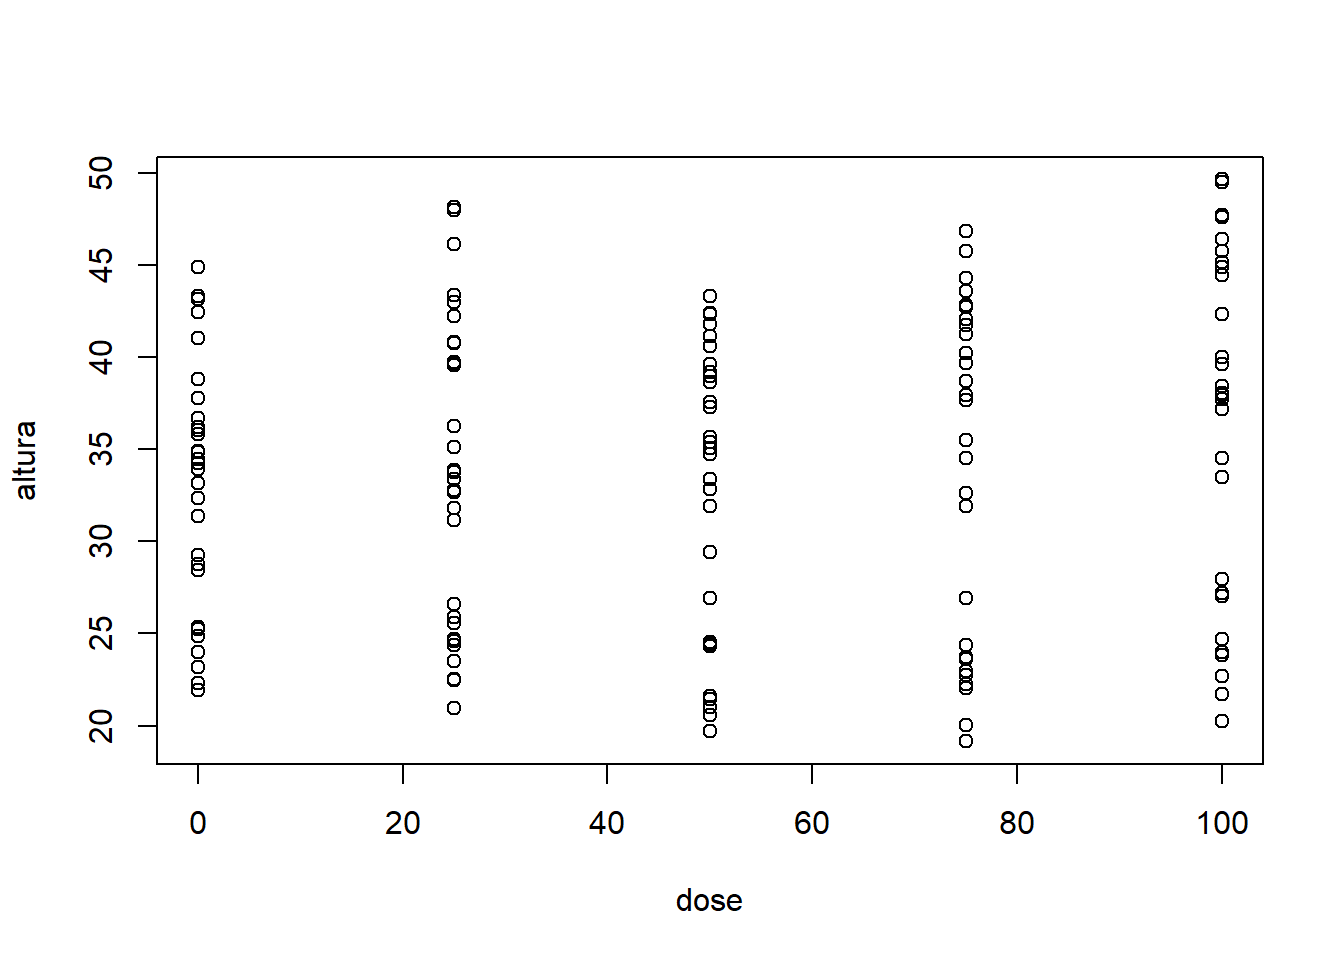
\includegraphics{bookdown_files/unnamed-chunk-98-1.png}

\begin{enumerate}
\def\labelenumi{\arabic{enumi}.}
\setcounter{enumi}{4}
\tightlist
\item
  Fixando concentracao igual a 20:
\end{enumerate}

\begin{Shaded}
\begin{Highlighting}[]
\KeywordTok{boxplot}\NormalTok{(}\DataTypeTok{data =}\NormalTok{ fatDIC2[fatDIC2}\OperatorTok{$}\NormalTok{irrigacao }\OperatorTok{==}\StringTok{ }\DecValTok{20}\NormalTok{,], }
\NormalTok{        enraizamento }\OperatorTok{~}\StringTok{ }\NormalTok{substrato)}
\end{Highlighting}
\end{Shaded}

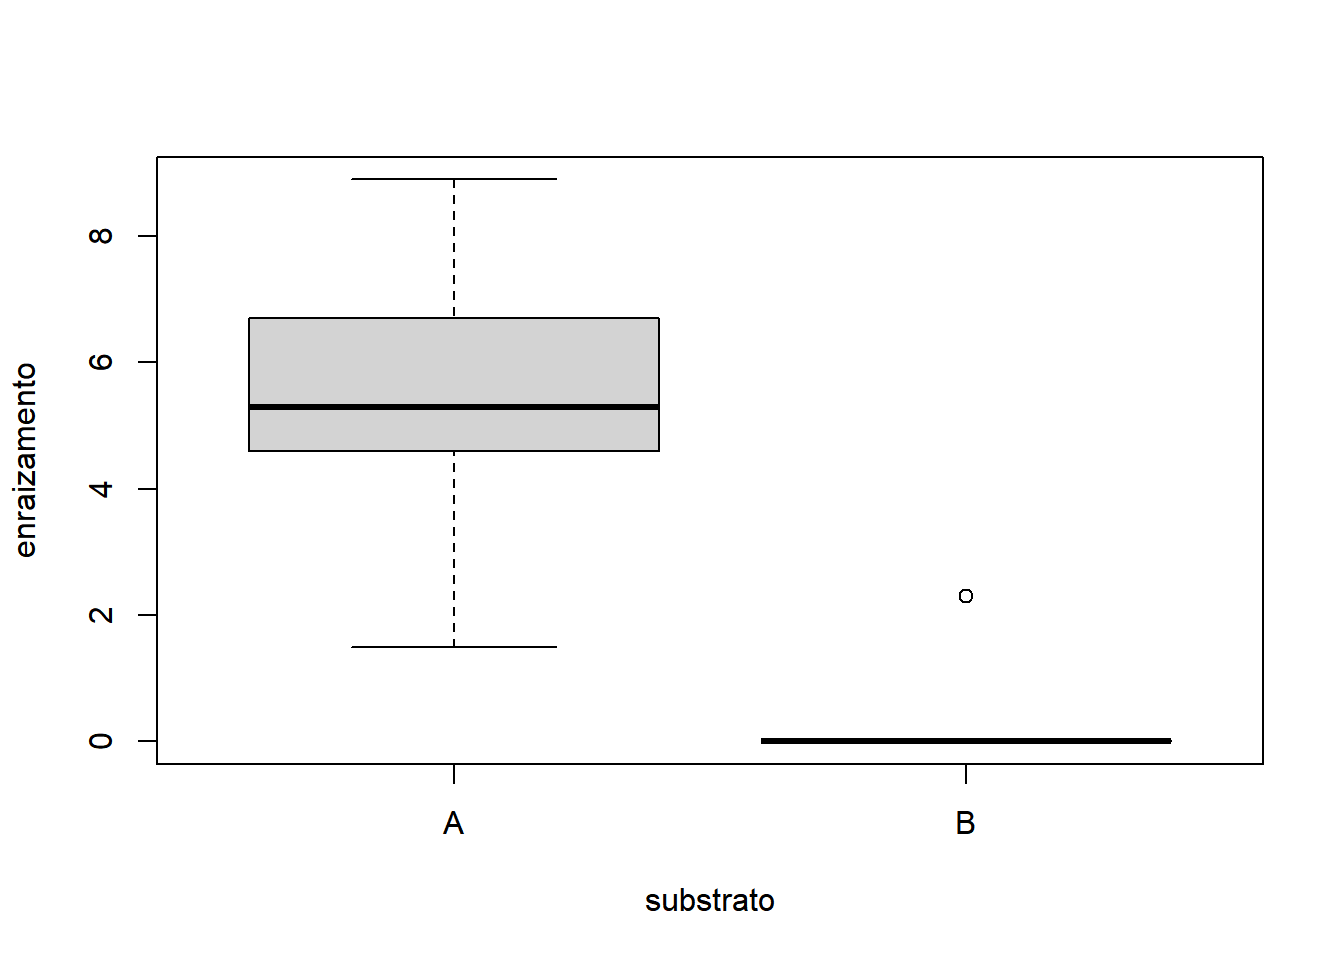
\includegraphics{bookdown_files/unnamed-chunk-99-1.png}

\begin{enumerate}
\def\labelenumi{\arabic{enumi}.}
\setcounter{enumi}{5}
\tightlist
\item
  Fixando Indutor igual a `A':
\end{enumerate}

\begin{Shaded}
\begin{Highlighting}[]
\KeywordTok{boxplot}\NormalTok{(}\DataTypeTok{data =}\NormalTok{ fatDIC2[fatDIC2}\OperatorTok{$}\NormalTok{substrato }\OperatorTok{==}\StringTok{ "A"}\NormalTok{,], }
\NormalTok{        enraizamento }\OperatorTok{~}\StringTok{ }\NormalTok{irrigacao)}
\end{Highlighting}
\end{Shaded}

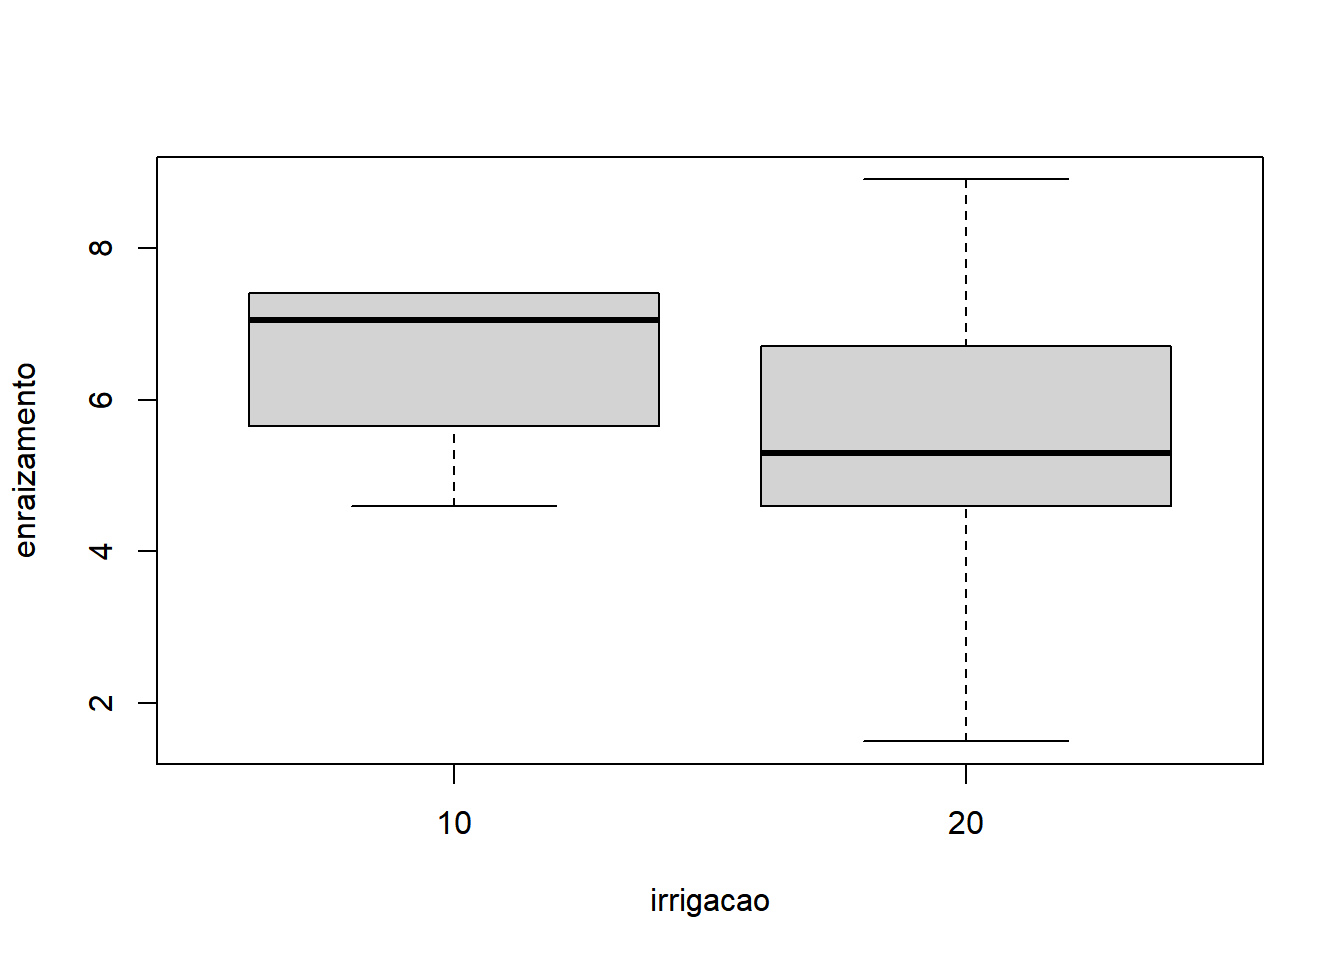
\includegraphics{bookdown_files/unnamed-chunk-100-1.png}

\begin{enumerate}
\def\labelenumi{\arabic{enumi}.}
\setcounter{enumi}{6}
\tightlist
\item
  Fixando Indutor igual a `B':
\end{enumerate}

\begin{Shaded}
\begin{Highlighting}[]
\KeywordTok{boxplot}\NormalTok{(}\DataTypeTok{data =}\NormalTok{ fatDIC2[fatDIC2}\OperatorTok{$}\NormalTok{substrato }\OperatorTok{==}\StringTok{ "B"}\NormalTok{,], }
\NormalTok{        enraizamento }\OperatorTok{~}\StringTok{ }\NormalTok{irrigacao)}
\end{Highlighting}
\end{Shaded}

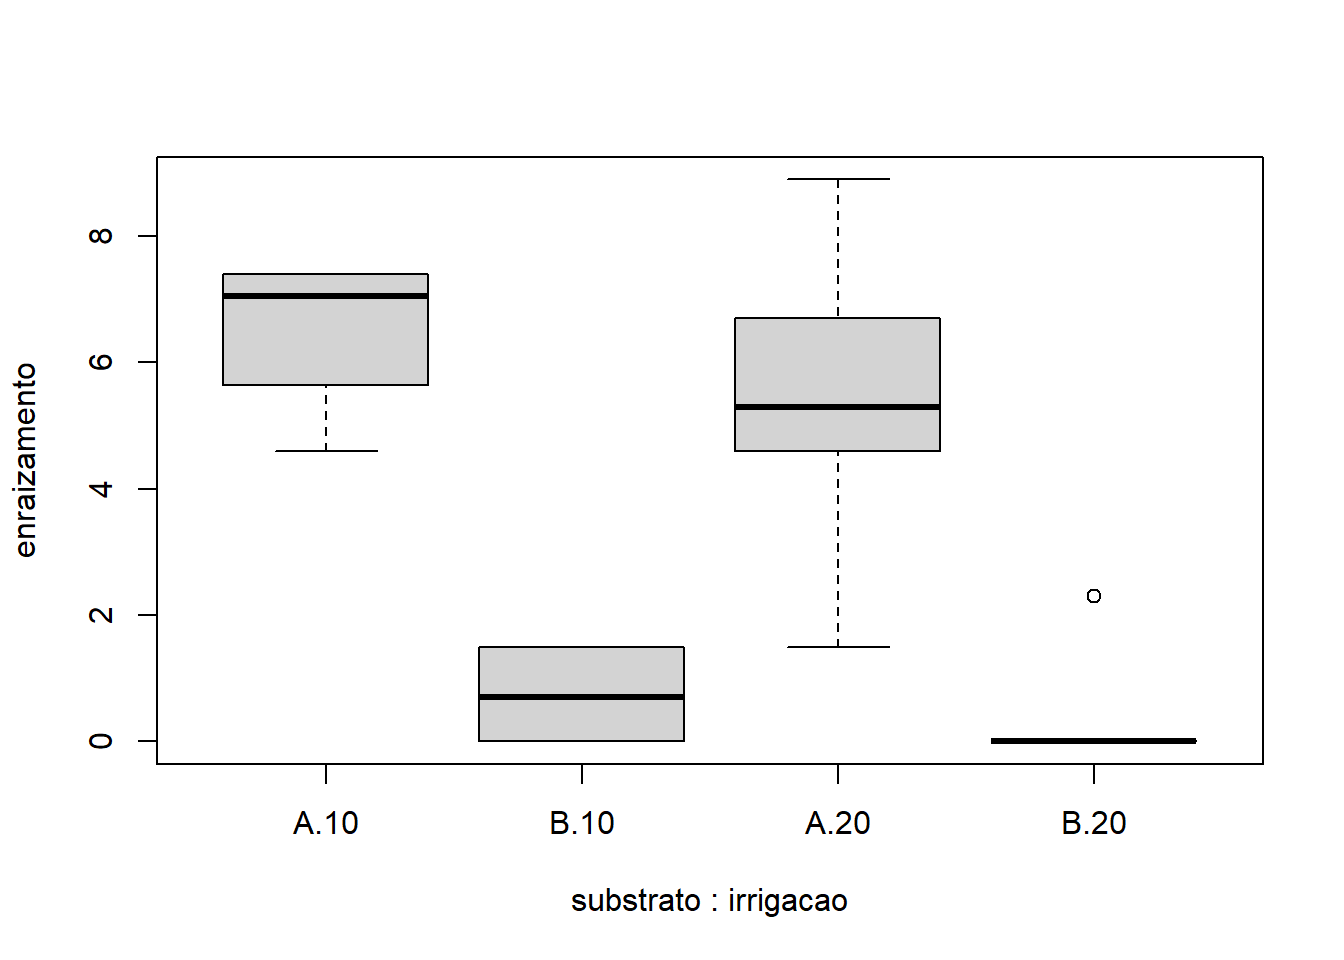
\includegraphics{bookdown_files/unnamed-chunk-101-1.png}

Os gráficos mostram que é razoável apontar que o fator substrato apresentou maior variação do que o fator irrigacao. A interação não parece influenciar o comportamento já identificado pelos fatores, quando analisados isoladamente. Sendo o nosso experimento desbalanceado, a função para rodar a ANOVA do tipo III é o \texttt{ea2()} (do pacote \texttt{easyanova}). A sintaxe da função é:

\begin{Shaded}
\begin{Highlighting}[]
\KeywordTok{ea2}\NormalTok{(data, }\DataTypeTok{design =} \DecValTok{1}\NormalTok{, }\DataTypeTok{alpha =} \FloatTok{0.05}\NormalTok{, }\DataTypeTok{cov =} \DecValTok{4}\NormalTok{, }\DataTypeTok{list =} \OtherTok{FALSE}\NormalTok{, }\DataTypeTok{p.adjust=}\DecValTok{1}\NormalTok{, }\DataTypeTok{plot=}\DecValTok{2}\NormalTok{)}
\end{Highlighting}
\end{Shaded}

Como já mencionado, o pacote \texttt{easyanova} exige que os dados sejam apresentados numa forma específica contendo apenas as colunas relevantes para a análise. No caso de um experimento fatorial duplo inteiramente casualizado, a ordem esperada das colunas é:

\begin{enumerate}
\def\labelenumi{\arabic{enumi}.}
\tightlist
\item
  Fator A
\item
  Fator B
\item
  Variável resposta
\end{enumerate}

Considerando as colunas \texttt{substrato}, \texttt{irrigacao} e \texttt{enraizamento} do dataframe \texttt{fatDIC2}. Os demais parâmetros da função \texttt{ea2()} serão definidos como \texttt{design\ =\ 1} e \texttt{plot\ =\ 2}.

\begin{Shaded}
\begin{Highlighting}[]
\KeywordTok{require}\NormalTok{(easyanova)}
\NormalTok{r.aov =}\StringTok{ }\KeywordTok{ea2}\NormalTok{(fatDIC2[, }\KeywordTok{c}\NormalTok{(}\DecValTok{1}\NormalTok{, }\DecValTok{2}\NormalTok{, }\DecValTok{4}\NormalTok{)], }\DataTypeTok{design =} \DecValTok{1}\NormalTok{)}
\end{Highlighting}
\end{Shaded}

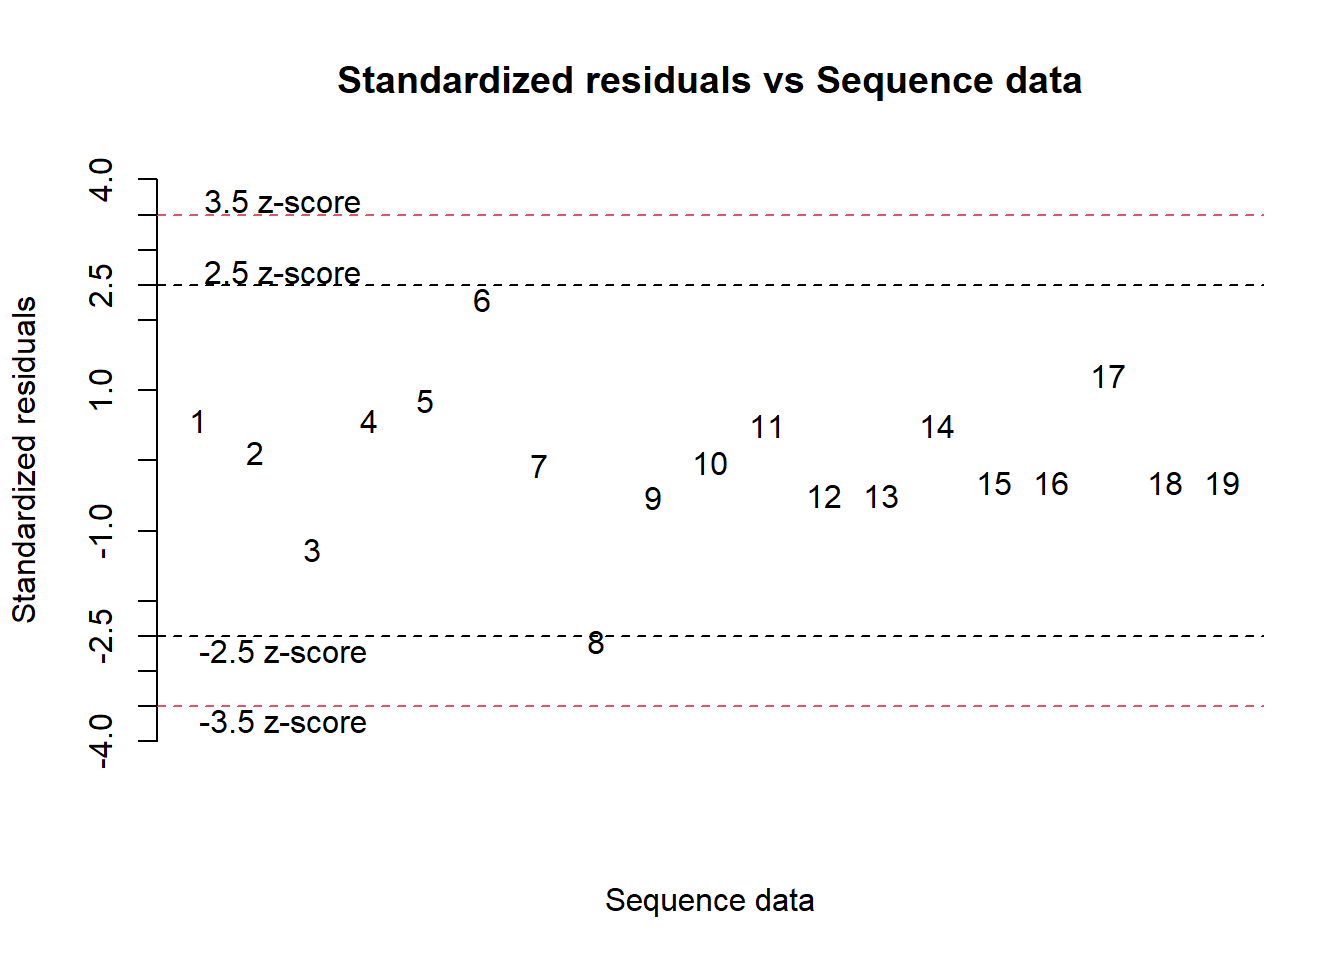
\includegraphics{bookdown_files/unnamed-chunk-103-1.png}

A saída da função \texttt{ea2()} é uma lista contendo os seguintes resultados:

\begin{Shaded}
\begin{Highlighting}[]
\KeywordTok{names}\NormalTok{(r.aov)}
\end{Highlighting}
\end{Shaded}

\begin{verbatim}
##  [1] "Analysis of variance"                                     
##  [2] "Adjusted means (factor 1)"                                
##  [3] "Multiple comparison test (factor 1)"                      
##  [4] "Adjusted means (factor 2)"                                
##  [5] "Multiple comparison test (factor 2)"                      
##  [6] "Adjusted means (factor 1 in levels of factor 2)"          
##  [7] "Multiple comparison test (factor 1 in levels of factor 2)"
##  [8] "Adjusted means (factor 2 in levels of factor 1)"          
##  [9] "Multiple comparison test (factor 2 in levels of factor 1)"
## [10] "Residual analysis"
\end{verbatim}

A lista acima contém os seguintes resultados:

\begin{enumerate}
\def\labelenumi{\arabic{enumi}.}
\tightlist
\item
  Análise de variância
\item
  Comparação de médias do fator 1
\item
  Teste de comparação múltipla do fator 1
\item
  Comparação de médias do fator 2\\
\item
  Teste de comparação múltipla do fator 2
\item
  Comparação de médias do fator 1 dentro dos níveis do fator 2
\item
  Teste de comparação múltipla do fator 1 dentro dos níveis do fator 2
\item
  Comparação de médias do fator 2 dentro dos níveis do fator 1
\item
  Teste de comparação múltipla do fator 2 dentro dos níveis do fator 1
\item
  Análise das pressuposições
\end{enumerate}

A primeira saída que deve ser verificada é a análise das pressuposições, na posição 10 da lista:

\begin{Shaded}
\begin{Highlighting}[]
\NormalTok{r.aov[}\DecValTok{10}\NormalTok{]}
\end{Highlighting}
\end{Shaded}

\begin{verbatim}
## $`Residual analysis`
## $`Residual analysis`$`residual analysis`
##                                     values
## p.value Shapiro-Wilk test           0.2084
## p.value Bartlett test (factor_1)    0.0146
## p.value Bartlett test (factor_2)    0.0610
## p.value Bartlett test (treatments)  0.0765
## coefficient of variation (%)       53.5100
## first value most discrepant         8.0000
## second value most discrepant        6.0000
## third value most discrepant         3.0000
## 
## $`Residual analysis`$residuals
##      1      2      3      4      5      6      7 
##  0.875  0.175 -1.925  0.875  1.300  3.500 -0.100 
##      8      9     10     11     12     13     14 
## -3.900 -0.800 -0.040  0.760 -0.740 -0.740  0.760 
##     15     16     17     18     19 
## -0.460 -0.460  1.840 -0.460 -0.460 
## 
## $`Residual analysis`$`standardized residuals`
##           1           2           3           4 
##  0.57590514  0.11518103 -1.26699130  0.57590514 
##           5           6           7           8 
##  0.85563049  2.30362055 -0.06581773 -2.56689147 
##           9          10          11          12 
## -0.52654184 -0.02632709  0.50021475 -0.48705120 
##          13          14          15          16 
## -0.48705120  0.50021475 -0.30276156 -0.30276156 
##          17          18          19 
##  1.21104623 -0.30276156 -0.30276156
\end{verbatim}

O teste de normalidade Shapiro-Wilk indica que não há evidência suficientes para rejeitar a pressuposição de normalidade do modelo estatístico e o teste de homogeneidade de variâncias Bartlett para os tratamentos indica que as variâncias são homogêneas. Portanto, o modelo escolhido é adequado para representar o experimento analisado. Desta forma, a análise de variância contido na posição 1 da lista de resultados pode ser analisado:

\begin{Shaded}
\begin{Highlighting}[]
\NormalTok{r.aov[}\DecValTok{1}\NormalTok{]}
\end{Highlighting}
\end{Shaded}

\begin{verbatim}
## $`Analysis of variance`
##                   df type III SS mean square
## factor_1           1    135.3243    135.3243
## factor_2           1      2.3224      2.3224
## factor_1:factor_2  1      0.8400      0.8400
## residuals         15     41.5515      2.7701
##                   F value    p>F
## factor_1          48.8518 <0.001
## factor_2           0.8384 0.3743
## factor_1:factor_2  0.3032   0.59
## residuals               -      -
\end{verbatim}

O fator 1 (Indutor) foi significativo, apresentando teste F inferior a 1\%. Já o fator 2 (Concentração), bem como a interação não foram significativas. Como a interação não foi significativa, não há necessidade de desdobramento, e o fator 1 pode ser analisado diretamente. Lembrando que no exemplo apresentado, o fator 1 possui apenas dois níveis e portanto o teste F é conclusivo. De qualquer maneira, o teste de médias do fator 1 pode ser obtido na posição 2 da lista de resultado.

\begin{Shaded}
\begin{Highlighting}[]
\NormalTok{r.aov[}\DecValTok{2}\NormalTok{]}
\end{Highlighting}
\end{Shaded}

\begin{verbatim}
## $`Adjusted means (factor 1)`
##   factor_1 adjusted.mean standard.error tukey snk
## 1        A        5.9625         0.5582     a   a
## 2        B        0.6000         0.5263     b   b
##   duncan t scott_knott
## 1      a a           a
## 2      b b           b
\end{verbatim}

\hypertarget{fatorial-duplo-em-blocos-casualizados}{%
\section{Fatorial duplo em blocos casualizados}\label{fatorial-duplo-em-blocos-casualizados}}

No caso de um fatorial duplo em blocos casualizados, a ANOVA contará com cinco fontes de variação: uma fonte de variação conhecida atribuída ao bloco, outra fonte de variação conhecida determinada pelo tratamento A, outra fonte de variação conhecida determinada pelo tratamento B, outra fonte de variação conhecida determinada pela interação entre os dois tratamentos e uma quinta fonte de variação desconhecida determinada pelo resíduo. O modelo estatístico do delineamento fatorial duplo inteiramente casualizado é:

\[Y = \bar{Y} + BLOCO + TRAT_A + TRAT_B + (TRAT_A * TRAT_B) + Erro\]

De forma semelhante ao experimento fatorial inteiramente casualizado, o caso balanceado será analisado através do pacote \texttt{ExpDes.pt} (função \texttt{fat2.dbc()}). Já o caso desbalanceado será analisado pelo pacote \texttt{easyanova} (função \texttt{ea2()} e \texttt{design=2}).

\hypertarget{o-caso-balanceado-3}{%
\subsection{O caso balanceado}\label{o-caso-balanceado-3}}

O exemplo balanceado trata de um experimento no qual se avalia a altura de um experimento fatorial combinando cinco doses de um adubo nitrogenado com três espécies de árvores nativas da Mata Atlântica, organizados em 10 blocos:

\begin{itemize}
\tightlist
\item
  Fator 1: Doses de adubos 0, 25, 50, 75 e 100
\item
  Fator 2: Espécies 2, 5 e 7
\item
  10 blocos
\item
  Variável de interesse: altura das plantas
\end{itemize}

\begin{table}

\caption{\label{tab:unnamed-chunk-108}Dados de experimento em fatorial DBC}
\centering
\begin{tabular}[t]{r|r|r|r}
\hline
dose & especie & bloco & altura\\
\hline
100 & 2 & 1 & 27.01093\\
\hline
100 & 2 & 2 & 24.67664\\
\hline
100 & 2 & 3 & 20.25999\\
\hline
100 & 2 & 4 & 23.98435\\
\hline
100 & 2 & 5 & 21.68730\\
\hline
100 & 2 & 6 & 27.95062\\
\hline
100 & 2 & 7 & 21.72693\\
\hline
100 & 2 & 8 & 23.81819\\
\hline
100 & 2 & 9 & 27.20599\\
\hline
100 & 2 & 10 & 22.71426\\
\hline
75 & 2 & 1 & 23.59123\\
\hline
75 & 2 & 2 & 22.25759\\
\hline
75 & 2 & 3 & 22.05516\\
\hline
75 & 2 & 4 & 20.04109\\
\hline
75 & 2 & 5 & 19.14948\\
\hline
75 & 2 & 6 & 22.95754\\
\hline
75 & 2 & 7 & 26.94884\\
\hline
75 & 2 & 8 & 22.74460\\
\hline
75 & 2 & 9 & 23.71342\\
\hline
75 & 2 & 10 & 24.38227\\
\hline
50 & 2 & 1 & 26.91505\\
\hline
50 & 2 & 2 & 19.72285\\
\hline
50 & 2 & 3 & 20.55555\\
\hline
50 & 2 & 4 & 24.44992\\
\hline
50 & 2 & 5 & 21.59082\\
\hline
50 & 2 & 6 & 24.56422\\
\hline
50 & 2 & 7 & 21.44374\\
\hline
50 & 2 & 8 & 20.99752\\
\hline
50 & 2 & 9 & 21.44592\\
\hline
50 & 2 & 10 & 24.29815\\
\hline
25 & 2 & 1 & 24.58642\\
\hline
25 & 2 & 2 & 22.54323\\
\hline
25 & 2 & 3 & 25.88379\\
\hline
25 & 2 & 4 & 23.48752\\
\hline
25 & 2 & 5 & 24.38289\\
\hline
25 & 2 & 6 & 24.72294\\
\hline
25 & 2 & 7 & 26.58771\\
\hline
25 & 2 & 8 & 22.46470\\
\hline
25 & 2 & 9 & 25.58907\\
\hline
25 & 2 & 10 & 20.94828\\
\hline
0 & 2 & 1 & 29.28761\\
\hline
0 & 2 & 2 & 24.83846\\
\hline
0 & 2 & 3 & 21.91967\\
\hline
0 & 2 & 4 & 25.25512\\
\hline
0 & 2 & 5 & 23.20428\\
\hline
0 & 2 & 6 & 22.30722\\
\hline
0 & 2 & 7 & 28.45246\\
\hline
0 & 2 & 8 & 25.35863\\
\hline
0 & 2 & 9 & 23.99814\\
\hline
0 & 2 & 10 & 28.78995\\
\hline
100 & 5 & 1 & 33.49074\\
\hline
100 & 5 & 2 & 37.72860\\
\hline
100 & 5 & 3 & 37.97029\\
\hline
100 & 5 & 4 & 39.65706\\
\hline
100 & 5 & 5 & 38.07058\\
\hline
100 & 5 & 6 & 38.46334\\
\hline
100 & 5 & 7 & 37.21368\\
\hline
100 & 5 & 8 & 40.00952\\
\hline
100 & 5 & 9 & 34.51427\\
\hline
100 & 5 & 10 & 38.46156\\
\hline
75 & 5 & 1 & 32.64211\\
\hline
75 & 5 & 2 & 42.87033\\
\hline
75 & 5 & 3 & 35.50921\\
\hline
75 & 5 & 4 & 34.52205\\
\hline
75 & 5 & 5 & 31.95030\\
\hline
75 & 5 & 6 & 40.25084\\
\hline
75 & 5 & 7 & 37.94206\\
\hline
75 & 5 & 8 & 41.28099\\
\hline
75 & 5 & 9 & 37.70441\\
\hline
75 & 5 & 10 & 39.68077\\
\hline
50 & 5 & 1 & 32.82667\\
\hline
50 & 5 & 2 & 31.92334\\
\hline
50 & 5 & 3 & 33.38743\\
\hline
50 & 5 & 4 & 29.40074\\
\hline
50 & 5 & 5 & 35.69536\\
\hline
50 & 5 & 6 & 38.64929\\
\hline
50 & 5 & 7 & 35.42279\\
\hline
50 & 5 & 8 & 34.72498\\
\hline
50 & 5 & 9 & 37.29969\\
\hline
50 & 5 & 10 & 35.06832\\
\hline
25 & 5 & 1 & 33.39860\\
\hline
25 & 5 & 2 & 39.56000\\
\hline
25 & 5 & 3 & 33.79608\\
\hline
25 & 5 & 4 & 33.88220\\
\hline
25 & 5 & 5 & 32.77403\\
\hline
25 & 5 & 6 & 31.14461\\
\hline
25 & 5 & 7 & 32.67330\\
\hline
25 & 5 & 8 & 31.84332\\
\hline
25 & 5 & 9 & 36.28326\\
\hline
25 & 5 & 10 & 35.10899\\
\hline
0 & 5 & 1 & 35.81985\\
\hline
0 & 5 & 2 & 36.19184\\
\hline
0 & 5 & 3 & 33.15076\\
\hline
0 & 5 & 4 & 33.92754\\
\hline
0 & 5 & 5 & 34.88189\\
\hline
0 & 5 & 6 & 34.25457\\
\hline
0 & 5 & 7 & 32.33597\\
\hline
0 & 5 & 8 & 31.39240\\
\hline
0 & 5 & 9 & 34.48195\\
\hline
0 & 5 & 10 & 35.83106\\
\hline
100 & 7 & 1 & 47.71383\\
\hline
100 & 7 & 2 & 45.75887\\
\hline
100 & 7 & 3 & 46.42036\\
\hline
100 & 7 & 4 & 44.89556\\
\hline
100 & 7 & 5 & 45.16561\\
\hline
100 & 7 & 6 & 44.48361\\
\hline
100 & 7 & 7 & 42.32970\\
\hline
100 & 7 & 8 & 49.53137\\
\hline
100 & 7 & 9 & 49.66715\\
\hline
100 & 7 & 10 & 47.61306\\
\hline
75 & 7 & 1 & 42.71420\\
\hline
75 & 7 & 2 & 42.74941\\
\hline
75 & 7 & 3 & 41.76867\\
\hline
75 & 7 & 4 & 44.32072\\
\hline
75 & 7 & 5 & 43.60612\\
\hline
75 & 7 & 6 & 38.70690\\
\hline
75 & 7 & 7 & 45.79070\\
\hline
75 & 7 & 8 & 42.08179\\
\hline
75 & 7 & 9 & 46.88940\\
\hline
75 & 7 & 10 & 45.78247\\
\hline
50 & 7 & 1 & 42.39296\\
\hline
50 & 7 & 2 & 38.98789\\
\hline
50 & 7 & 3 & 40.60666\\
\hline
50 & 7 & 4 & 39.63895\\
\hline
50 & 7 & 5 & 41.79340\\
\hline
50 & 7 & 6 & 42.35532\\
\hline
50 & 7 & 7 & 39.21753\\
\hline
50 & 7 & 8 & 41.16574\\
\hline
50 & 7 & 9 & 37.56872\\
\hline
50 & 7 & 10 & 43.35592\\
\hline
25 & 7 & 1 & 48.19243\\
\hline
25 & 7 & 2 & 43.00286\\
\hline
25 & 7 & 3 & 48.00344\\
\hline
25 & 7 & 4 & 40.75832\\
\hline
25 & 7 & 5 & 39.65651\\
\hline
25 & 7 & 6 & 46.13281\\
\hline
25 & 7 & 7 & 39.76537\\
\hline
25 & 7 & 8 & 43.41116\\
\hline
25 & 7 & 9 & 42.23041\\
\hline
25 & 7 & 10 & 40.82259\\
\hline
0 & 7 & 1 & 36.07182\\
\hline
0 & 7 & 2 & 43.15407\\
\hline
0 & 7 & 3 & 43.32585\\
\hline
0 & 7 & 4 & 37.79503\\
\hline
0 & 7 & 5 & 41.04694\\
\hline
0 & 7 & 6 & 44.91720\\
\hline
0 & 7 & 7 & 34.90952\\
\hline
0 & 7 & 8 & 42.47311\\
\hline
0 & 7 & 9 & 36.70185\\
\hline
0 & 7 & 10 & 38.83515\\
\hline
\end{tabular}
\end{table}

O primeiro passo é importar o arquivo contendo os resultados do experimento para dentro do R. Esta tarefa pode ser realizada através do seguinte comando:

\begin{Shaded}
\begin{Highlighting}[]
\NormalTok{fatDBC1 =}\StringTok{ }\KeywordTok{read.csv}\NormalTok{(}\StringTok{"./data/Experimento Fatorial Duplo DBC 1.csv"}\NormalTok{, }
                   \DataTypeTok{sep =} \StringTok{","}\NormalTok{, }\DataTypeTok{dec =} \StringTok{"."}\NormalTok{)}
\end{Highlighting}
\end{Shaded}

Para explorar este experimento graficamente, tanto a função \texttt{boxplot()} quanto a função \texttt{plot()} serão usadas. Isto ocorre porque o experimento apresenta um fator quantitativo (doses) e outro fator qualitativo (espécies). Assim, sempre que for analisado o efeito das doses, serão utilizar gráficos de dispersão. Enquanto que ao analisar o efeito dos clones, o boxplot será utilizado.

\begin{enumerate}
\def\labelenumi{\arabic{enumi}.}
\tightlist
\item
  Considerando apenas fator 1:
\end{enumerate}

\begin{Shaded}
\begin{Highlighting}[]
\KeywordTok{plot}\NormalTok{(}\DataTypeTok{data =}\NormalTok{ fatDBC1, altura }\OperatorTok{~}\StringTok{ }\NormalTok{dose)}
\end{Highlighting}
\end{Shaded}

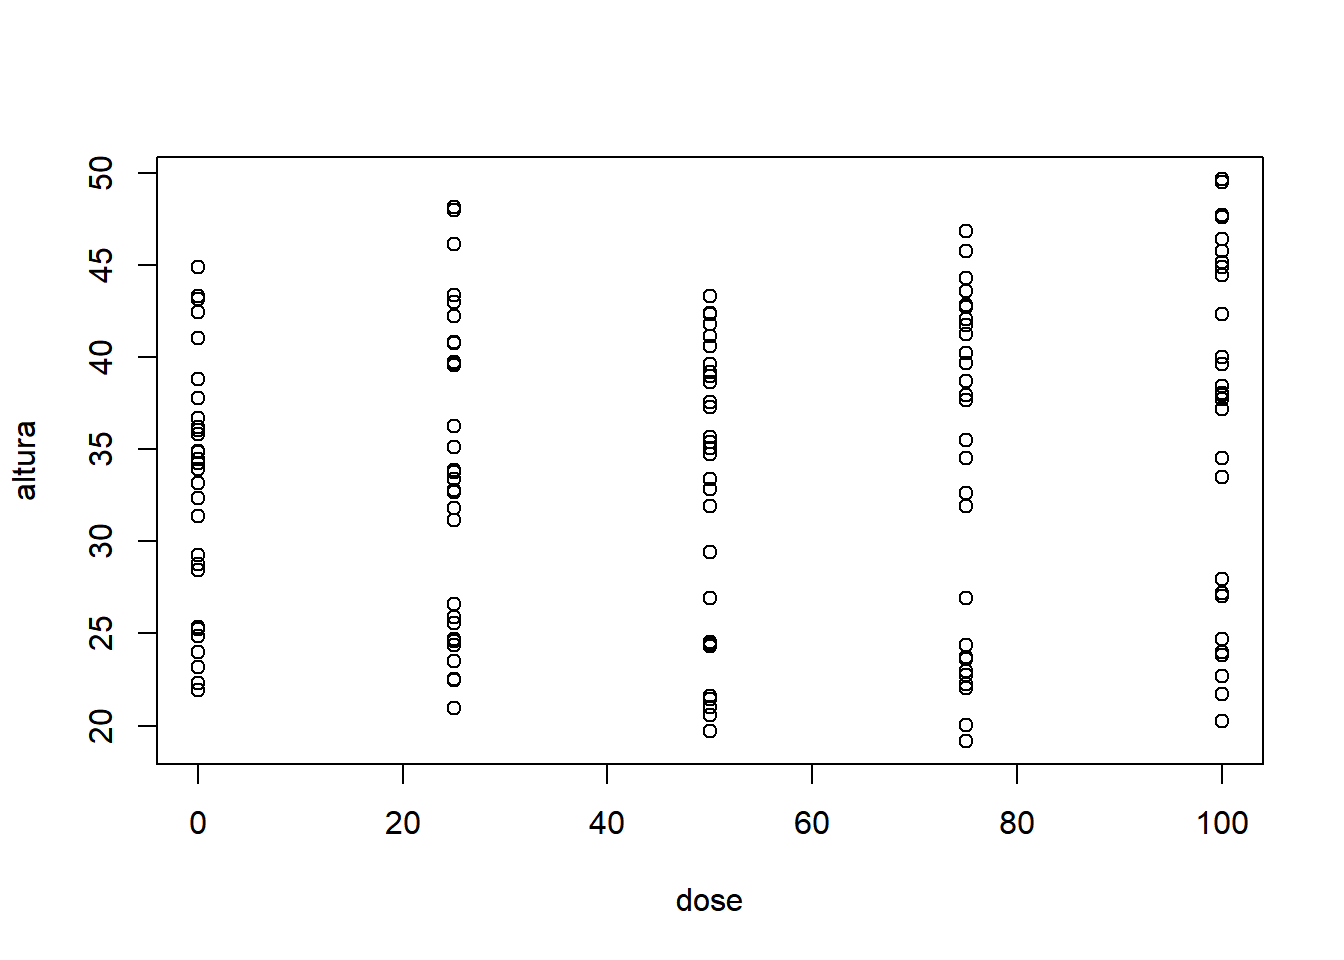
\includegraphics{bookdown_files/unnamed-chunk-110-1.png}

\begin{enumerate}
\def\labelenumi{\arabic{enumi}.}
\setcounter{enumi}{1}
\tightlist
\item
  Considerando apenas fator 2:
\end{enumerate}

\begin{Shaded}
\begin{Highlighting}[]
\KeywordTok{boxplot}\NormalTok{(}\DataTypeTok{data =}\NormalTok{ fatDBC1, altura }\OperatorTok{~}\StringTok{ }\NormalTok{especie)}
\end{Highlighting}
\end{Shaded}

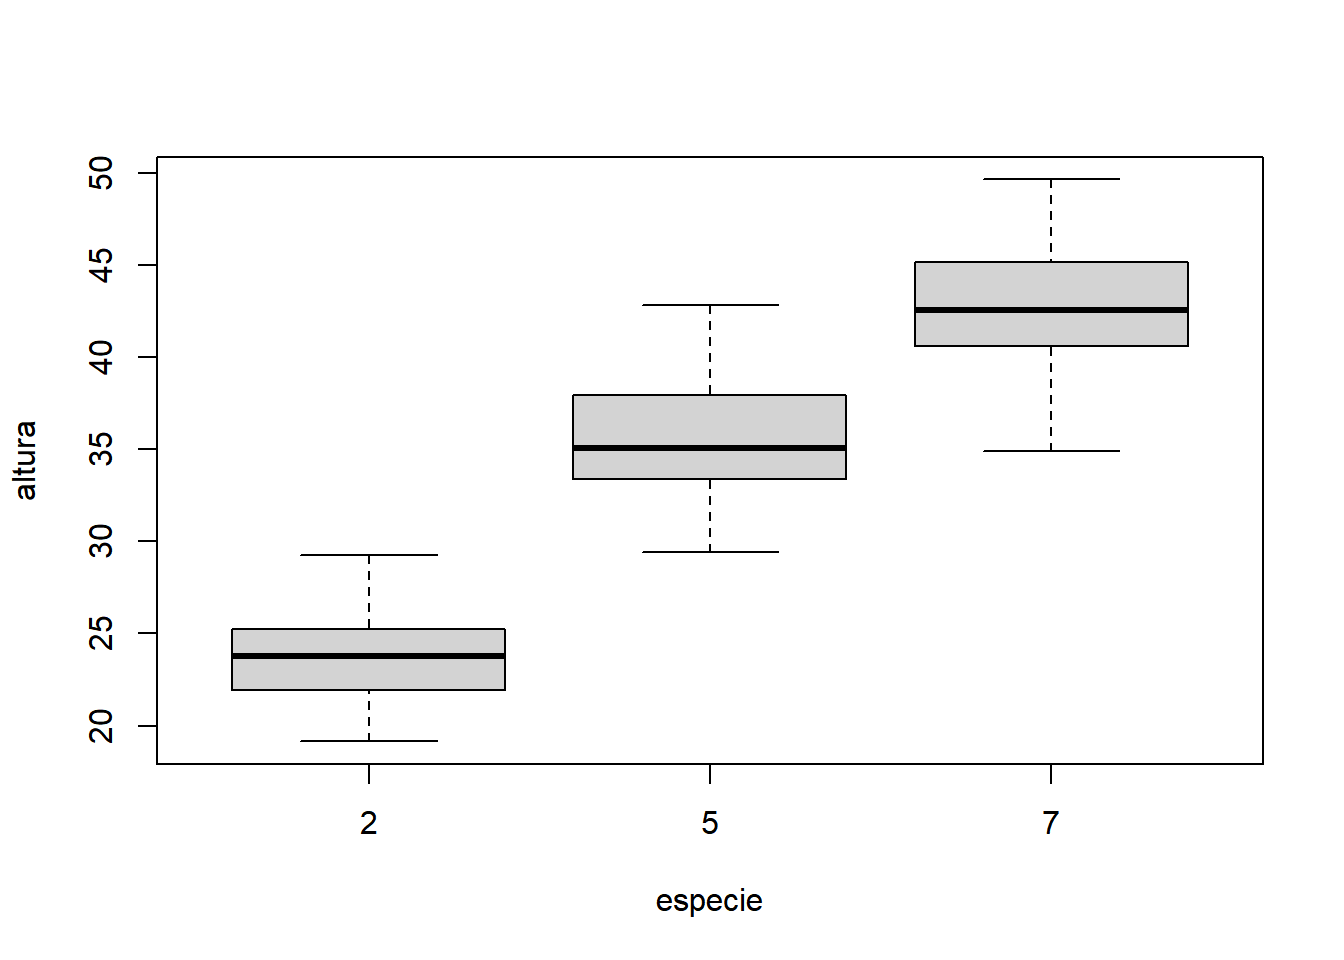
\includegraphics{bookdown_files/unnamed-chunk-111-1.png}

\begin{enumerate}
\def\labelenumi{\arabic{enumi}.}
\setcounter{enumi}{2}
\tightlist
\item
  Interação dos fatores:
\end{enumerate}

\begin{Shaded}
\begin{Highlighting}[]
\KeywordTok{boxplot}\NormalTok{(}\DataTypeTok{data =}\NormalTok{ fatDBC1, altura }\OperatorTok{~}\StringTok{ }\NormalTok{especie}\OperatorTok{/}\NormalTok{dose)}
\end{Highlighting}
\end{Shaded}

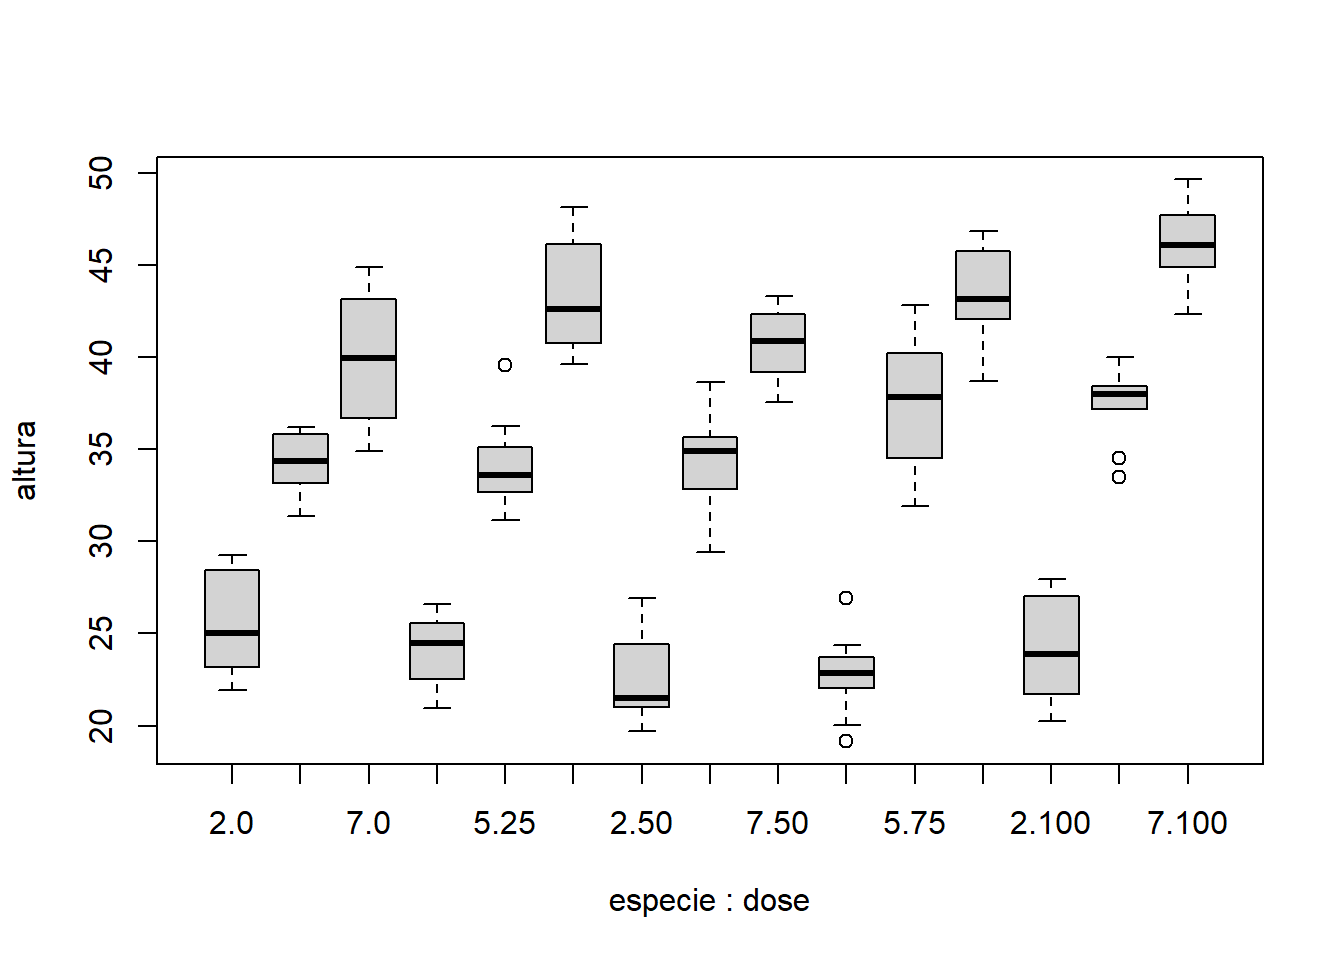
\includegraphics{bookdown_files/unnamed-chunk-112-1.png}

\begin{enumerate}
\def\labelenumi{\arabic{enumi}.}
\setcounter{enumi}{3}
\tightlist
\item
  Efeito dos blocos:
\end{enumerate}

\begin{Shaded}
\begin{Highlighting}[]
\KeywordTok{boxplot}\NormalTok{(}\DataTypeTok{data =}\NormalTok{ fatDBC1, altura }\OperatorTok{~}\StringTok{ }\NormalTok{especie}\OperatorTok{/}\NormalTok{bloco)}
\end{Highlighting}
\end{Shaded}

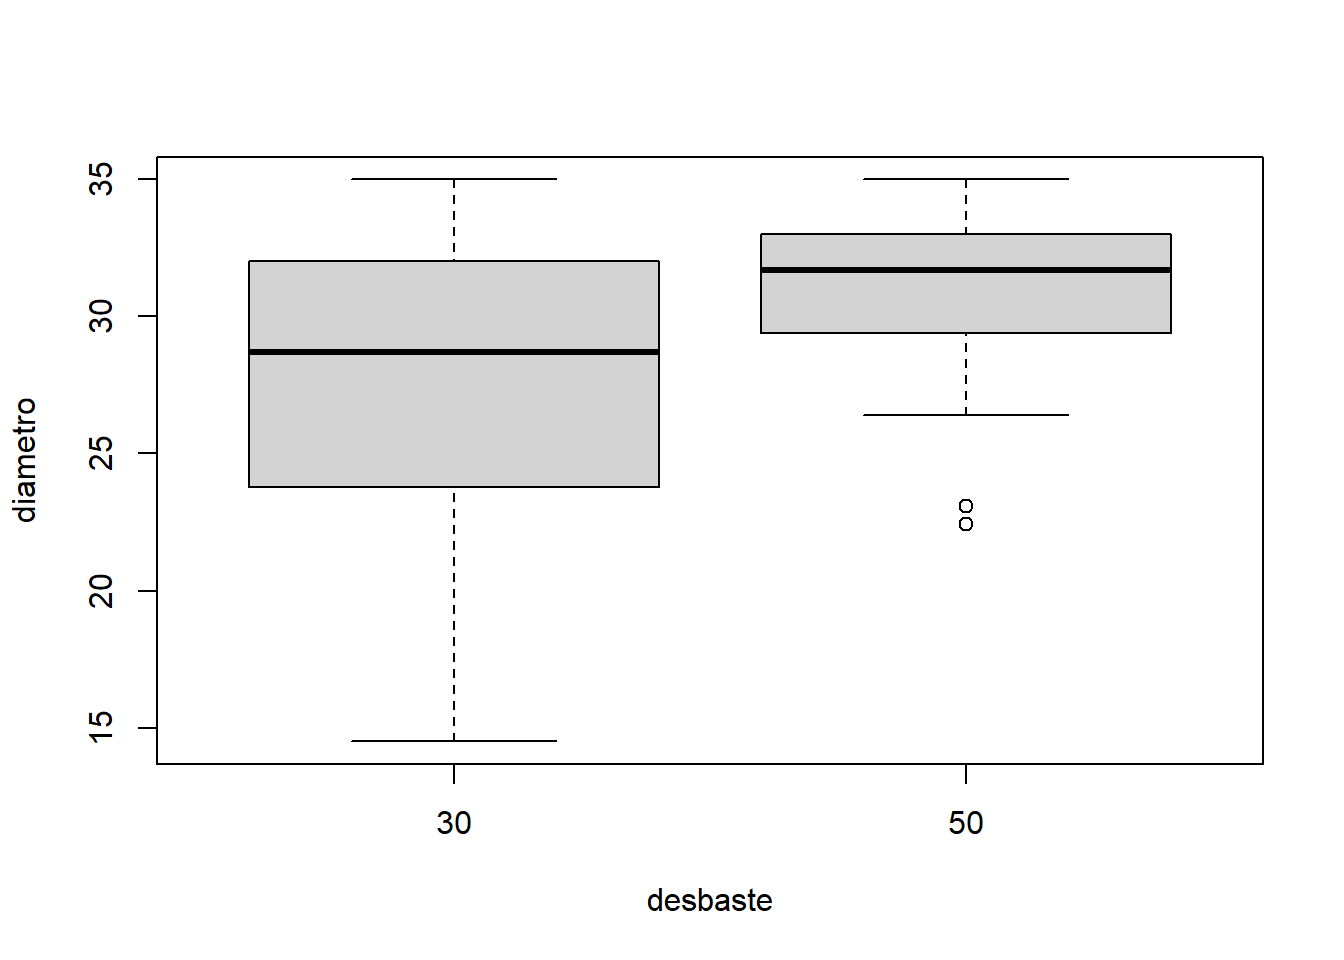
\includegraphics{bookdown_files/unnamed-chunk-113-1.png}

\begin{Shaded}
\begin{Highlighting}[]
\KeywordTok{boxplot}\NormalTok{(}\DataTypeTok{data =}\NormalTok{ fatDBC1, altura }\OperatorTok{~}\StringTok{ }\NormalTok{dose}\OperatorTok{/}\NormalTok{bloco)}
\end{Highlighting}
\end{Shaded}

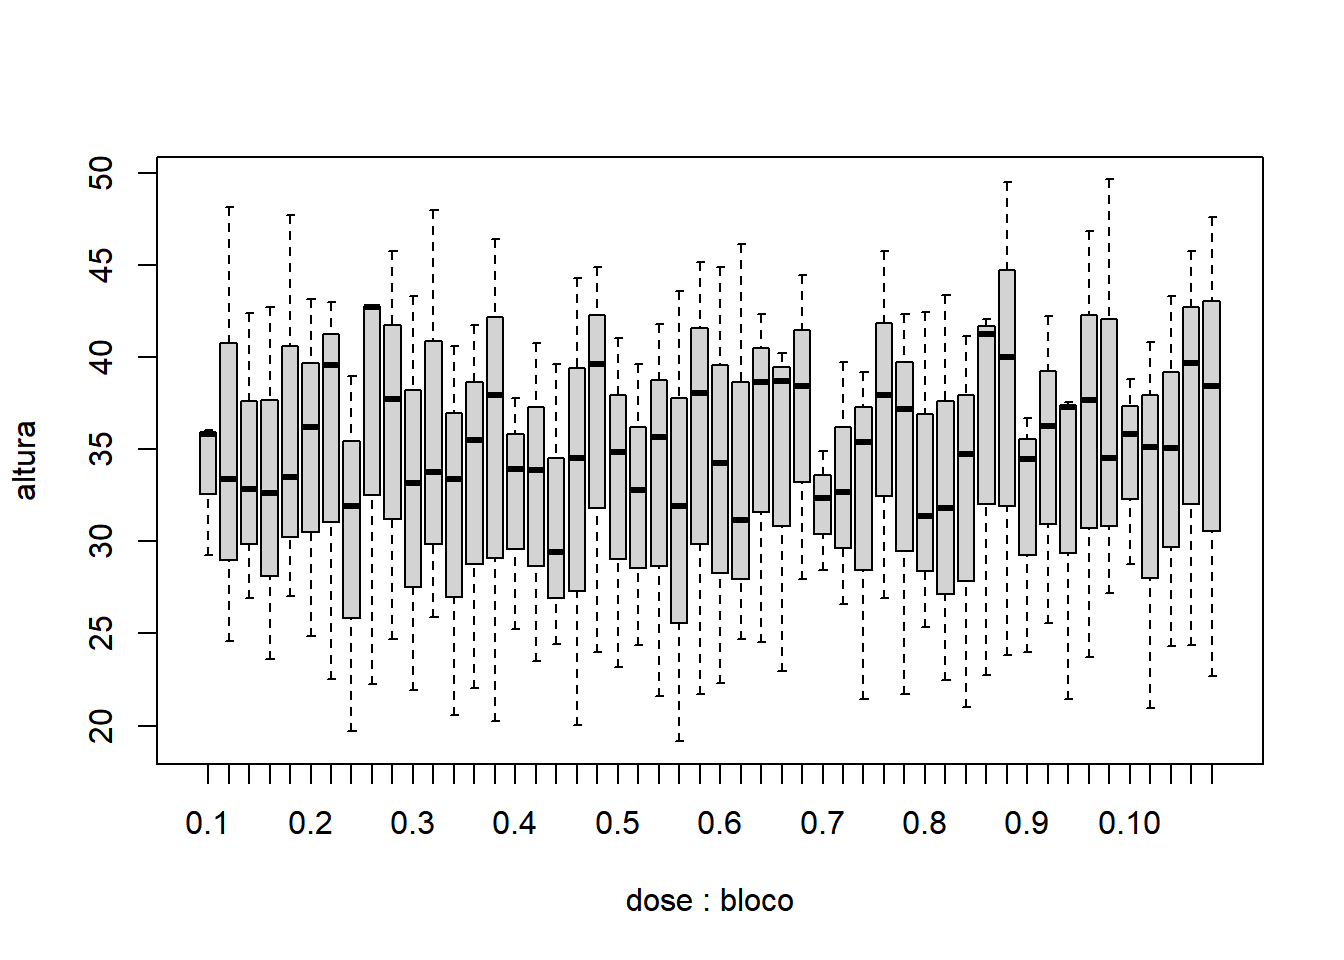
\includegraphics{bookdown_files/unnamed-chunk-113-2.png}

\begin{enumerate}
\def\labelenumi{\arabic{enumi}.}
\setcounter{enumi}{4}
\tightlist
\item
  Fixando especie igual a 2:
\end{enumerate}

\begin{Shaded}
\begin{Highlighting}[]
\KeywordTok{plot}\NormalTok{(}\DataTypeTok{data =}\NormalTok{ fatDBC1[fatDBC1}\OperatorTok{$}\NormalTok{especie }\OperatorTok{==}\StringTok{ }\DecValTok{2}\NormalTok{,], altura }\OperatorTok{~}\StringTok{ }\NormalTok{dose)}
\end{Highlighting}
\end{Shaded}

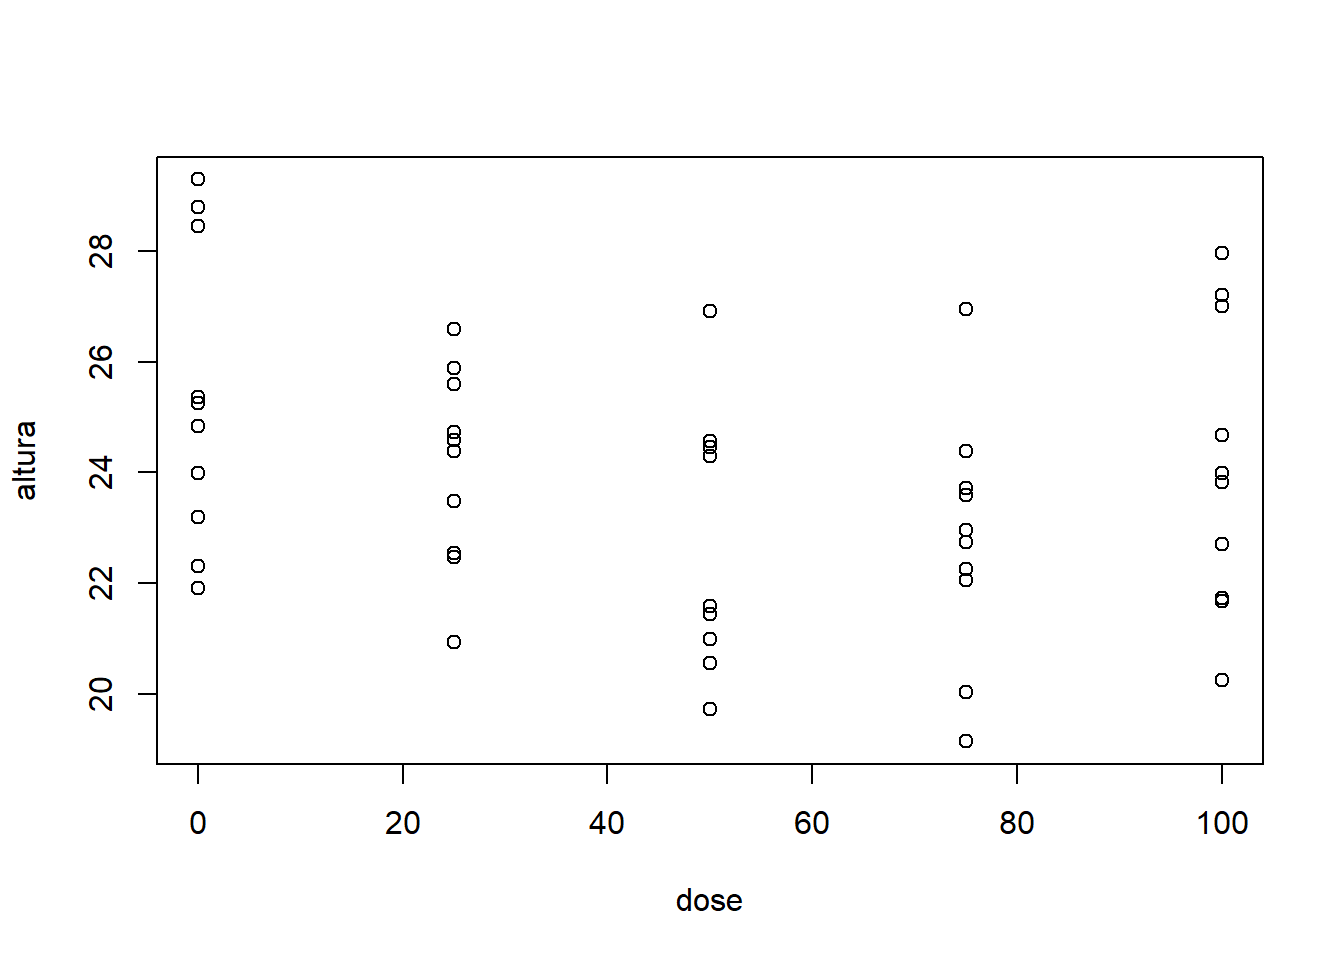
\includegraphics{bookdown_files/unnamed-chunk-114-1.png}

\begin{enumerate}
\def\labelenumi{\arabic{enumi}.}
\setcounter{enumi}{5}
\tightlist
\item
  Fixando especie igual a 5:
\end{enumerate}

\begin{Shaded}
\begin{Highlighting}[]
\KeywordTok{plot}\NormalTok{(}\DataTypeTok{data =}\NormalTok{ fatDBC1[fatDBC1}\OperatorTok{$}\NormalTok{especie }\OperatorTok{==}\StringTok{ }\DecValTok{5}\NormalTok{,], altura }\OperatorTok{~}\StringTok{ }\NormalTok{dose)}
\end{Highlighting}
\end{Shaded}

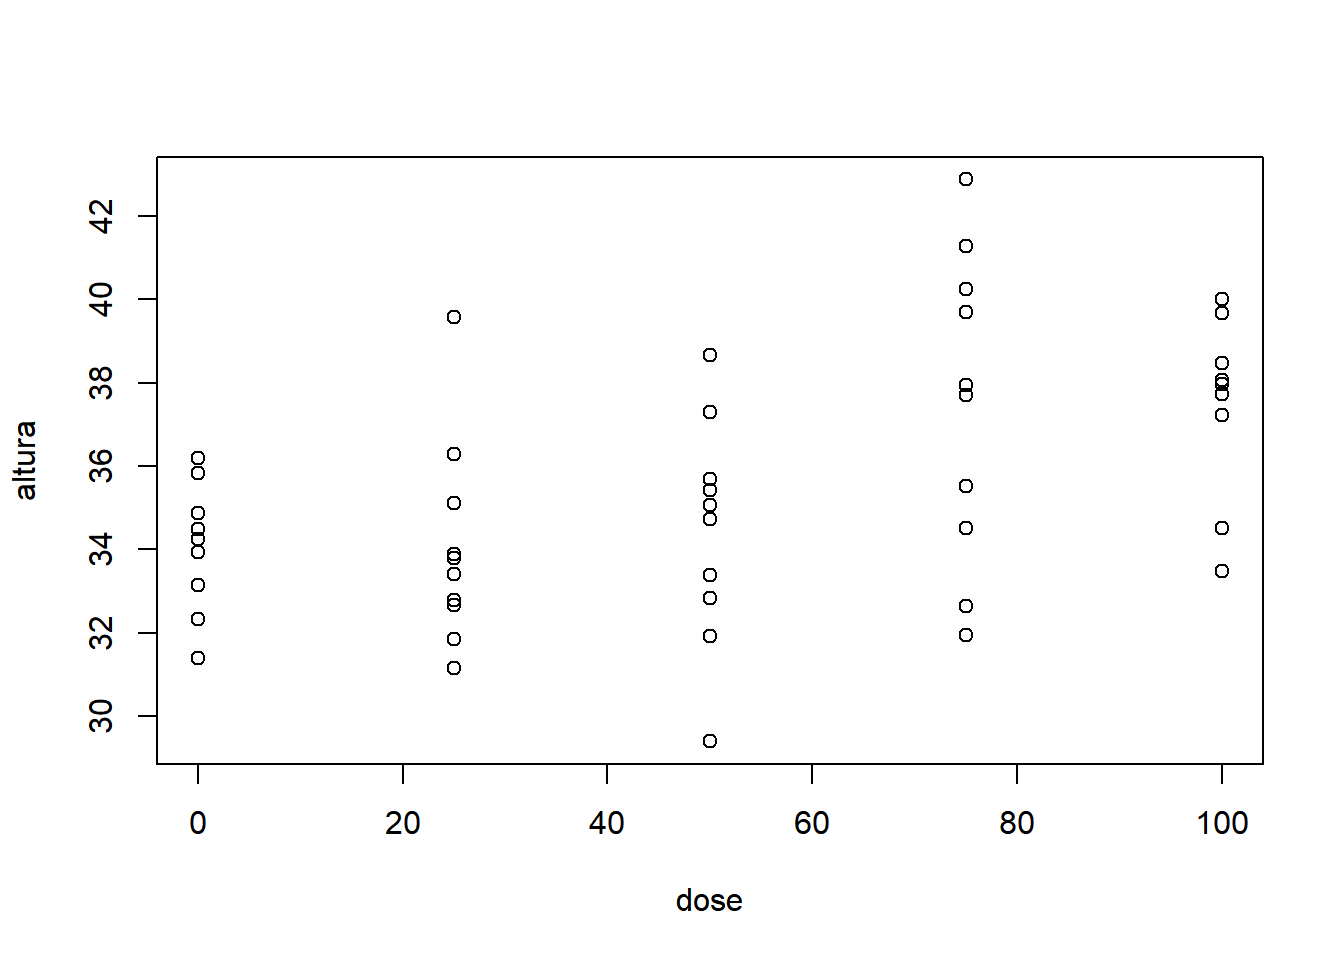
\includegraphics{bookdown_files/unnamed-chunk-115-1.png}

\begin{enumerate}
\def\labelenumi{\arabic{enumi}.}
\setcounter{enumi}{6}
\tightlist
\item
  Fixando especie igual a 7:
\end{enumerate}

\begin{Shaded}
\begin{Highlighting}[]
\KeywordTok{plot}\NormalTok{(}\DataTypeTok{data =}\NormalTok{ fatDBC1[fatDBC1}\OperatorTok{$}\NormalTok{especie }\OperatorTok{==}\StringTok{ }\DecValTok{7}\NormalTok{,], altura }\OperatorTok{~}\StringTok{ }\NormalTok{dose)}
\end{Highlighting}
\end{Shaded}

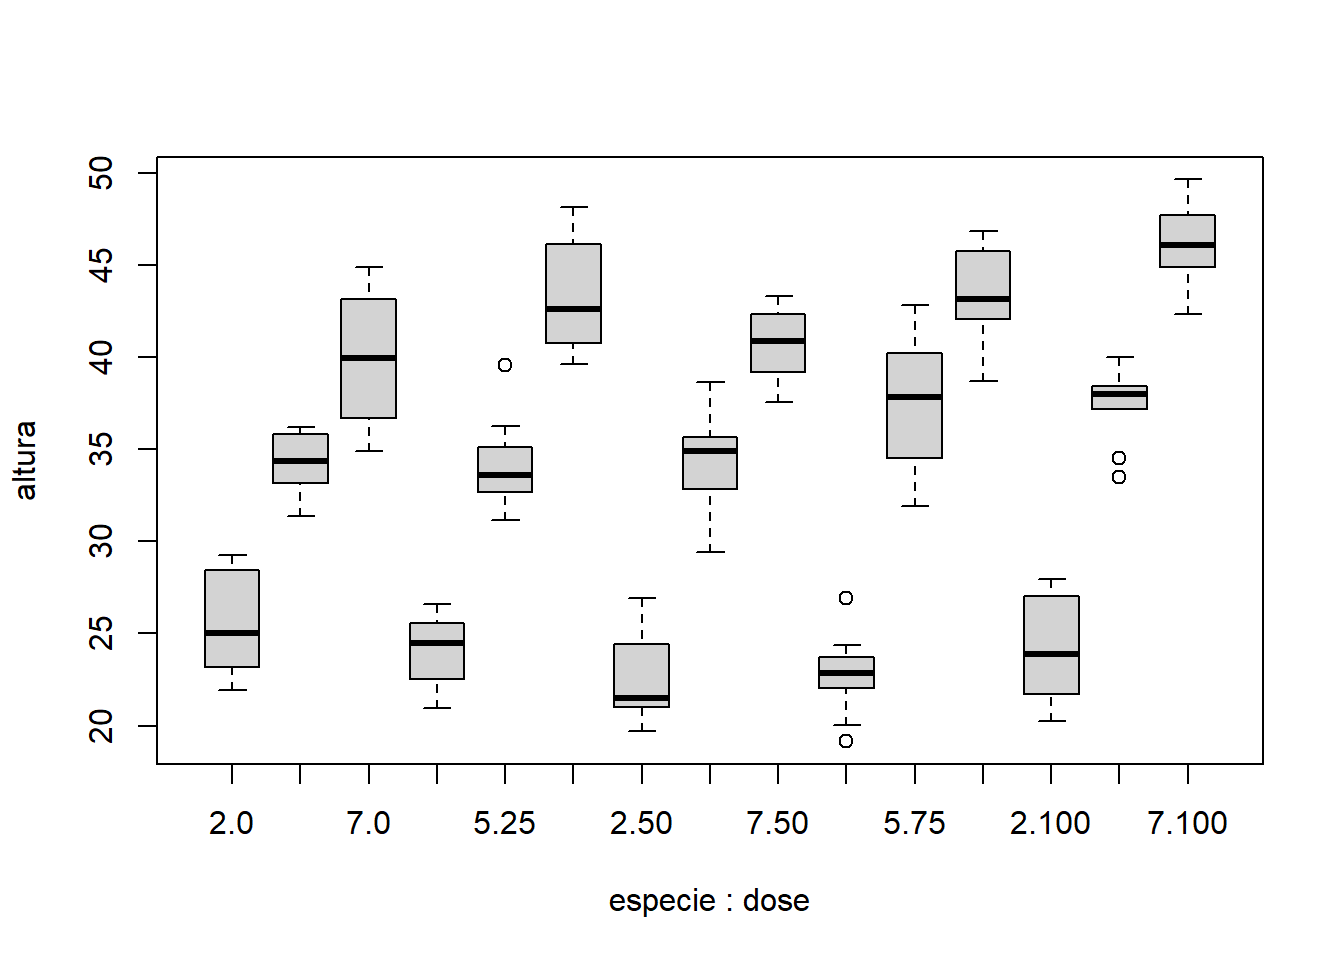
\includegraphics{bookdown_files/unnamed-chunk-116-1.png}

\begin{enumerate}
\def\labelenumi{\arabic{enumi}.}
\setcounter{enumi}{7}
\tightlist
\item
  Fixando dose igual a 0:
\end{enumerate}

\begin{Shaded}
\begin{Highlighting}[]
\KeywordTok{boxplot}\NormalTok{(}\DataTypeTok{data =}\NormalTok{ fatDBC1[fatDBC1}\OperatorTok{$}\NormalTok{dose }\OperatorTok{==}\StringTok{ }\DecValTok{0}\NormalTok{,], altura }\OperatorTok{~}\StringTok{ }\NormalTok{especie)}
\end{Highlighting}
\end{Shaded}

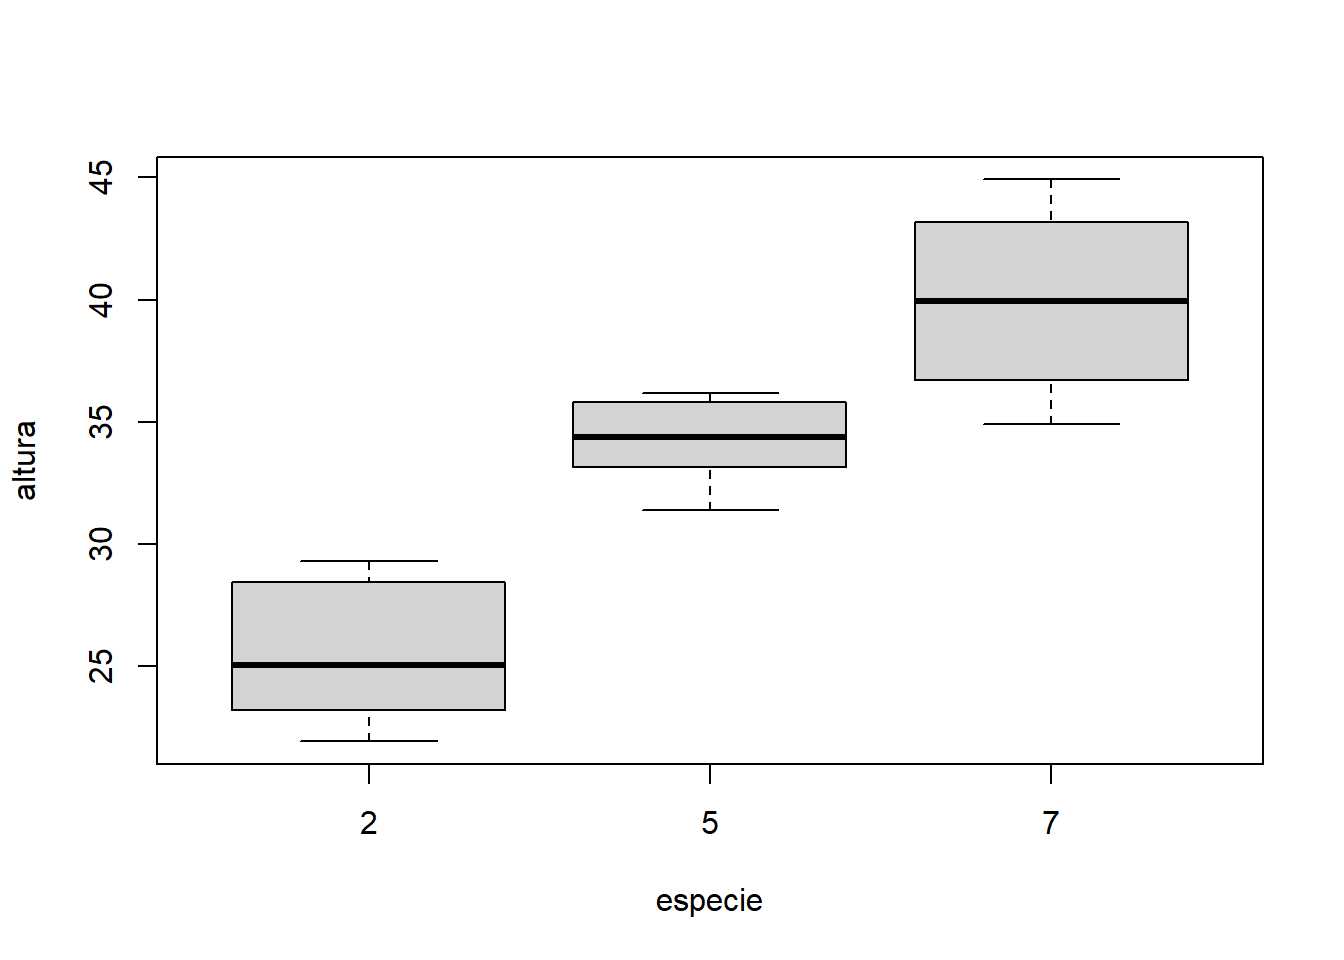
\includegraphics{bookdown_files/unnamed-chunk-117-1.png}

\begin{enumerate}
\def\labelenumi{\arabic{enumi}.}
\setcounter{enumi}{8}
\tightlist
\item
  Fixando dose igual a 25:
\end{enumerate}

\begin{Shaded}
\begin{Highlighting}[]
\KeywordTok{boxplot}\NormalTok{(}\DataTypeTok{data =}\NormalTok{ fatDBC1[fatDBC1}\OperatorTok{$}\NormalTok{dose }\OperatorTok{==}\StringTok{ }\DecValTok{25}\NormalTok{,], altura }\OperatorTok{~}\StringTok{ }\NormalTok{especie)}
\end{Highlighting}
\end{Shaded}

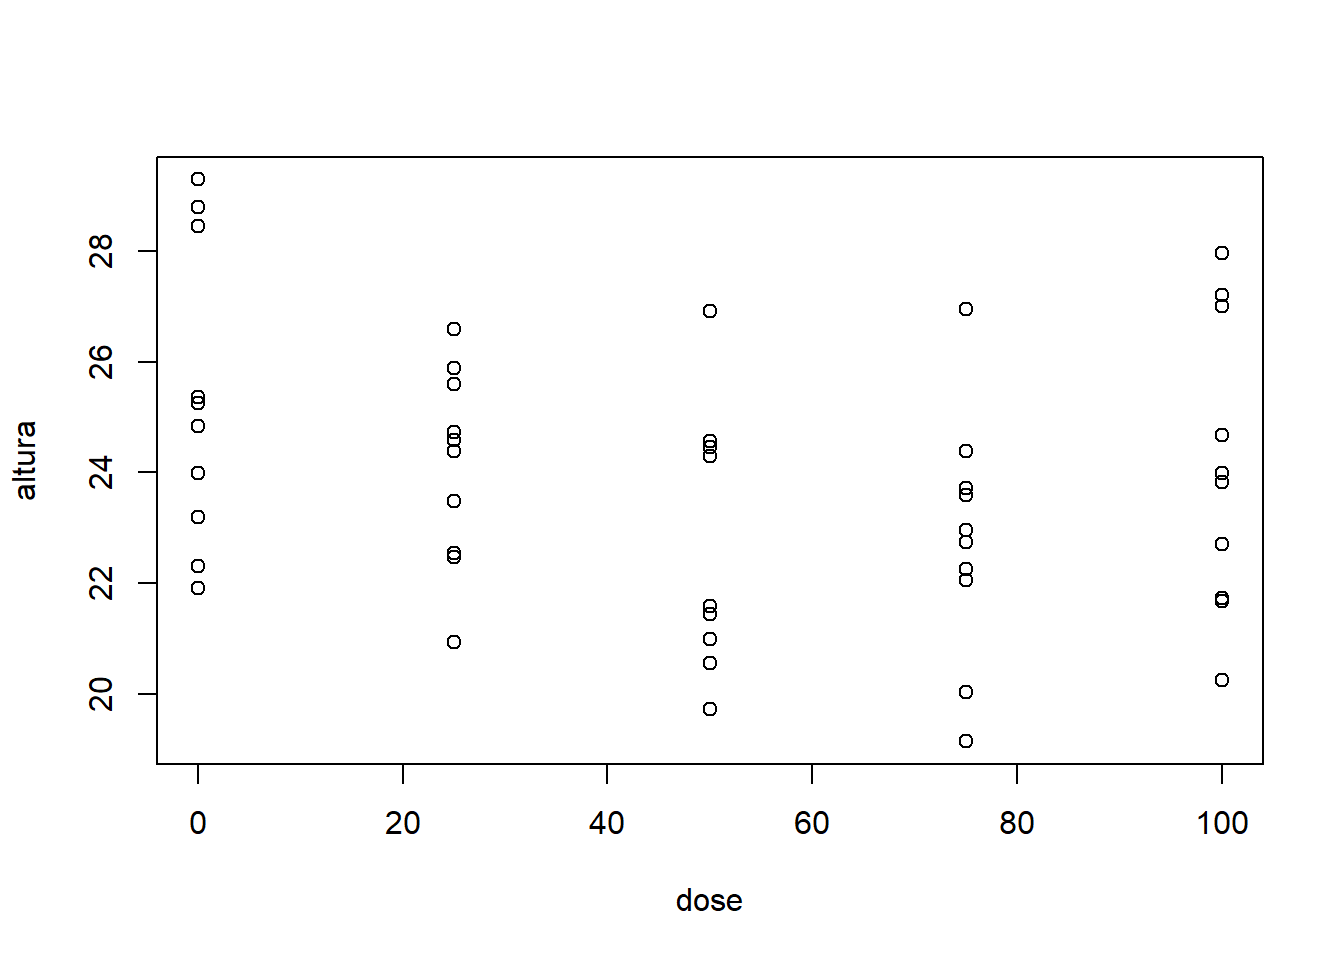
\includegraphics{bookdown_files/unnamed-chunk-118-1.png}

\begin{enumerate}
\def\labelenumi{\arabic{enumi}.}
\setcounter{enumi}{9}
\tightlist
\item
  Fixando dose igual a 50:
\end{enumerate}

\begin{Shaded}
\begin{Highlighting}[]
\KeywordTok{boxplot}\NormalTok{(}\DataTypeTok{data =}\NormalTok{ fatDBC1[fatDBC1}\OperatorTok{$}\NormalTok{dose }\OperatorTok{==}\StringTok{ }\DecValTok{50}\NormalTok{,], altura }\OperatorTok{~}\StringTok{ }\NormalTok{especie)}
\end{Highlighting}
\end{Shaded}

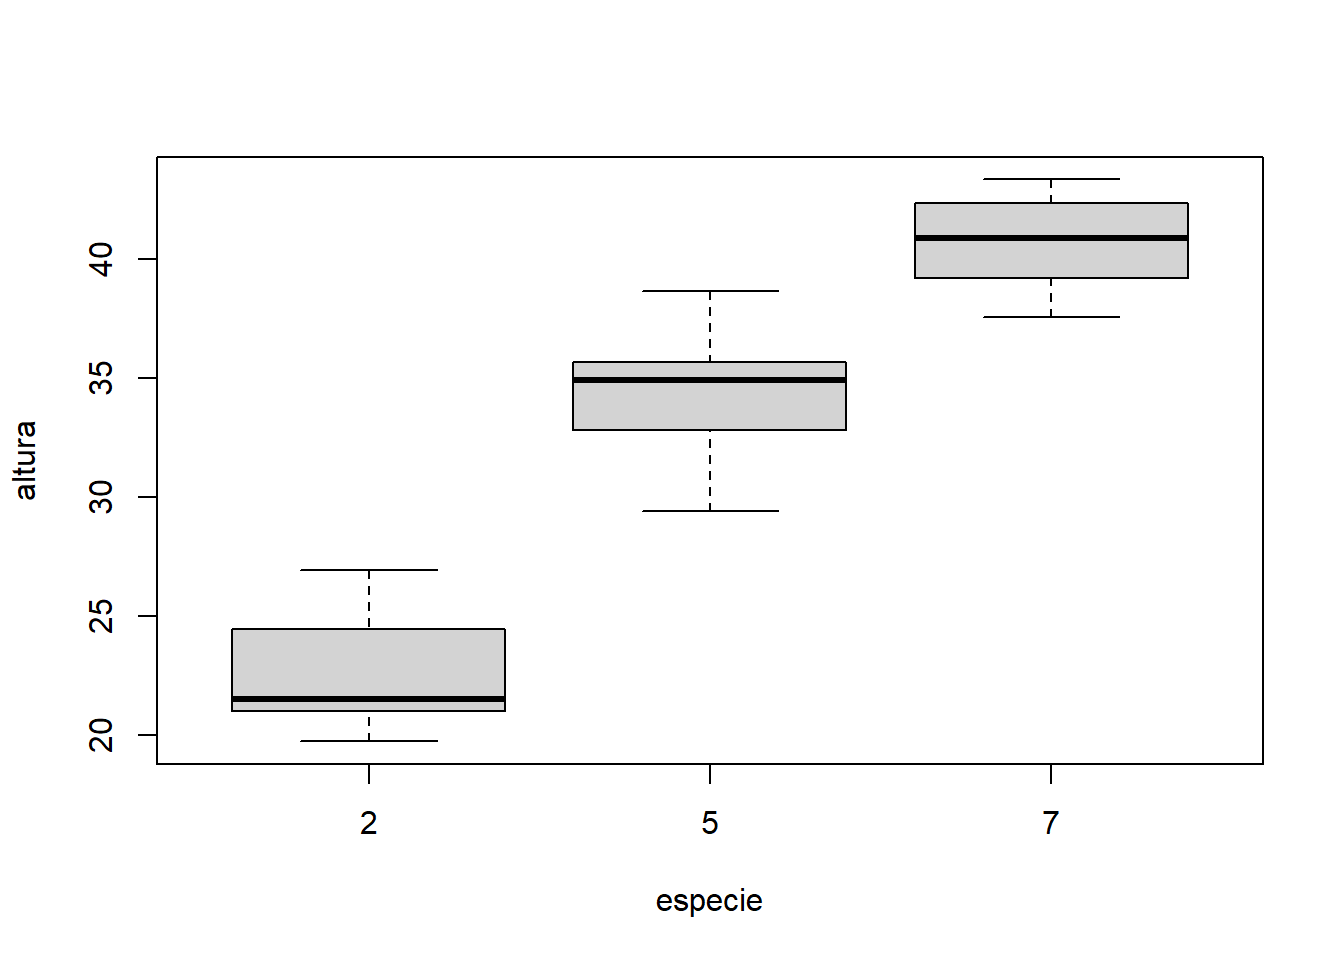
\includegraphics{bookdown_files/unnamed-chunk-119-1.png}

\begin{enumerate}
\def\labelenumi{\arabic{enumi}.}
\setcounter{enumi}{10}
\tightlist
\item
  Fixando dose igual a 75:
\end{enumerate}

\begin{Shaded}
\begin{Highlighting}[]
\KeywordTok{boxplot}\NormalTok{(}\DataTypeTok{data =}\NormalTok{ fatDBC1[fatDBC1}\OperatorTok{$}\NormalTok{dose }\OperatorTok{==}\StringTok{ }\DecValTok{75}\NormalTok{,], altura }\OperatorTok{~}\StringTok{ }\NormalTok{especie)}
\end{Highlighting}
\end{Shaded}

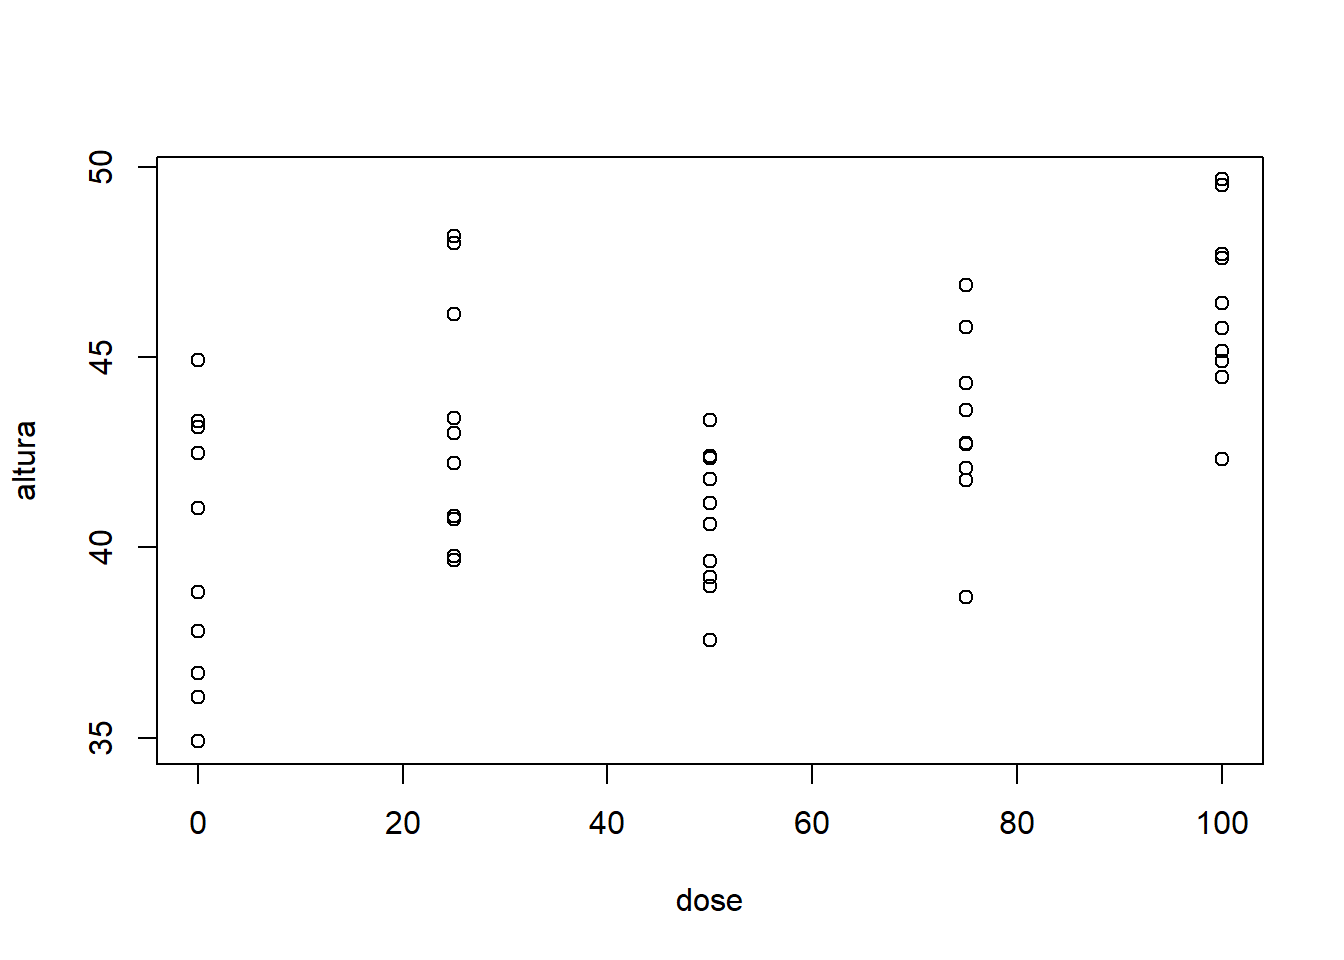
\includegraphics{bookdown_files/unnamed-chunk-120-1.png}

\begin{enumerate}
\def\labelenumi{\arabic{enumi}.}
\setcounter{enumi}{11}
\tightlist
\item
  Fixando dose igual a 100:
\end{enumerate}

\begin{Shaded}
\begin{Highlighting}[]
\KeywordTok{boxplot}\NormalTok{(}\DataTypeTok{data =}\NormalTok{ fatDBC1[fatDBC1}\OperatorTok{$}\NormalTok{dose }\OperatorTok{==}\StringTok{ }\DecValTok{100}\NormalTok{,], altura }\OperatorTok{~}\StringTok{ }\NormalTok{especie)}
\end{Highlighting}
\end{Shaded}

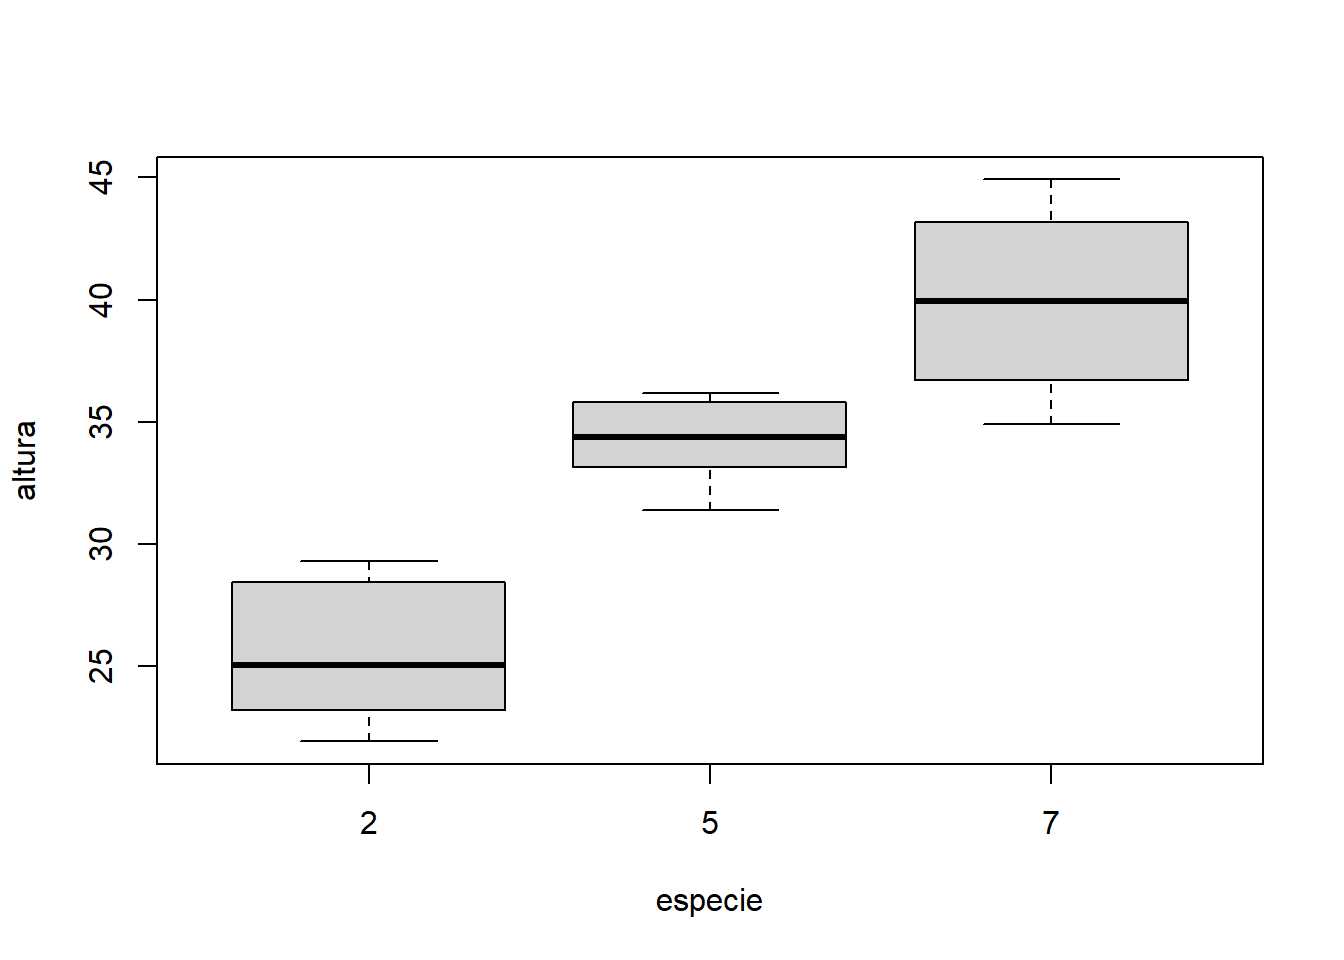
\includegraphics{bookdown_files/unnamed-chunk-121-1.png}

Com base nos gráficos apresentados, é razoável acreditar que há um efeito significativo da espécie, mas não fica muito evidente o efeito significativo da dose, da interação e do bloco. Nota-se que as doses possuem comportamentos diferentes, variando de uma tendência quadrática à uma tendência sigmoidal (cúbica).

Note que quanto mais fatores e interações estiverem presentes no experimento, mais complicado vai ficando a análise gráfica e também a análise estatística. E é por este motivo que desencoraja-se o uso de experimentos fatoriais triplos. Embora os pacotes de análise experimental possuam funções para experimentos fatoriais triplos, eles não serão apresentados aqui neste livro.

A análise estatística será feita pela função \texttt{fat2.dbc()} do pacote \texttt{ExpDes.pt}. A sintaxe básica da função pode ser vista acessando a página de ajuda da função:

\begin{Shaded}
\begin{Highlighting}[]
\KeywordTok{fat2.dbc}\NormalTok{(fator1, fator2, bloco, resp, }\DataTypeTok{quali =} \KeywordTok{c}\NormalTok{(}\OtherTok{TRUE}\NormalTok{, }\OtherTok{TRUE}\NormalTok{), }
         \DataTypeTok{mcomp =} \StringTok{"tukey"}\NormalTok{, }\DataTypeTok{fac.names =} \KeywordTok{c}\NormalTok{(}\StringTok{"F1"}\NormalTok{, }\StringTok{"F2"}\NormalTok{), }
         \DataTypeTok{sigT =} \FloatTok{0.05}\NormalTok{, }\DataTypeTok{sigF =} \FloatTok{0.05}\NormalTok{)}
\end{Highlighting}
\end{Shaded}

Lembrando que como se tem um fator quantitativo e um fator qualitativo, além dos parâmetros obrigatórios, será necessário ajustar o parâmetro \texttt{quali}:

\begin{Shaded}
\begin{Highlighting}[]
\KeywordTok{require}\NormalTok{(ExpDes.pt)}

\KeywordTok{fat2.dbc}\NormalTok{(fatDBC1}\OperatorTok{$}\NormalTok{dose, fatDBC1}\OperatorTok{$}\NormalTok{especie, fatDBC1}\OperatorTok{$}\NormalTok{bloco,}
\NormalTok{         fatDBC1}\OperatorTok{$}\NormalTok{altura, }\DataTypeTok{quali =} \KeywordTok{c}\NormalTok{(}\OtherTok{FALSE}\NormalTok{, }\OtherTok{TRUE}\NormalTok{), }
         \DataTypeTok{fac.names =} \KeywordTok{c}\NormalTok{(}\StringTok{"Dose"}\NormalTok{, }\StringTok{"Espécie"}\NormalTok{))}
\end{Highlighting}
\end{Shaded}

\begin{verbatim}
## ------------------------------------------------------------------------
## Legenda:
## FATOR 1:  Dose 
## FATOR 2:  Espécie 
## ------------------------------------------------------------------------
## 
## 
## Quadro da analise de variancia
## ------------------------------------------------------------------------
##               GL      SQ     QM     Fc   Pr>Fc
## Bloco          9    60.5    6.7   1.03 0.41738
## Dose           4   212.6   53.1   8.16 0.00001
## Espécie        2  9138.4 4569.2 702.07 0.00000
## Dose*Espécie   8   224.7   28.1   4.32 0.00013
## Residuo      126   820.0    6.5               
## Total        149 10456.2                      
## ------------------------------------------------------------------------
## CV = 7.5 %
## 
## ------------------------------------------------------------------------
## Teste de normalidade dos residuos (Shapiro-Wilk)
## valor-p:  0.6115979 
## De acordo com o teste de Shapiro-Wilk a 5% de significancia, os residuos podem ser considerados normais.
## ------------------------------------------------------------------------
## 
## 
## 
## Interacao significativa: desdobrando a interacao
## ------------------------------------------------------------------------
## 
## Desdobrando  Dose  dentro de cada nivel de  Espécie 
## ------------------------------------------------------------------------
## ------------------------------------------------------------------------
## Quadro da analise de variancia
## ------------------------------------------------------------------------
##                 GL          SQ         QM      Fc
## Bloco            9    60.52166    6.72463  1.0333
## Espécie          2  9138.36405 4569.18202 702.069
## Dose:Espécie 2   4    50.44803   12.61201  1.9379
## Dose:Espécie 5   4   128.29922   32.07481  4.9284
## Dose:Espécie 7   4   258.52025   64.63006  9.9306
## Residuo        126   820.02899    6.50817        
## Total          149 10456.18221   70.17572        
##                 Pr.Fc
## Bloco          0.4174
## Espécie        0.0000
## Dose:Espécie 2 0.1082
## Dose:Espécie 5 0.0010
## Dose:Espécie 7 0.0000
## Residuo            NA
## Total              NA
## ------------------------------------------------------------------------
## 
## 
## 
##  Dose  dentro do nivel  2  de  Espécie 
## 
## De acordo com o teste F, as medias desse fator sao estatisticamente iguais.
## ------------------------------------------------------------------------
##     Niveis     Medias
## 1        0   25.34115
## 2      100   24.10352
## 3       25   24.11965
## 4       50   22.59837
## 5       75   22.78412
## ------------------------------------------------------------------------
## 
## 
##  Dose  dentro do nivel  5  de  Espécie 
## ------------------------------------------------------------------------
## Ajuste de modelos polinomiais de regressao
## ------------------------------------------------------------------------
## 
## Modelo Linear
## =========================================
##    Estimativa Erro.padrao   tc    valor.p
## -----------------------------------------
## b0  33.5310     0.6249    53.6589    0   
## b1   0.0402     0.0102    3.9399  0.0001 
## -----------------------------------------
## 
## R2 do modelo linear
## --------
## 0.787434
## --------
## 
## Analise de variancia do modelo linear
## ========================================================
##                      GL     SQ       QM     Fc   valor.p
## --------------------------------------------------------
## Efeito linear         1  101.0272 101.0272 15.52 0.00013
## Desvios de Regressao  3  27.2720   9.0907   1.4  0.24689
## Residuos             126 820.0290  6.5082               
## --------------------------------------------------------
## ------------------------------------------------------------------------
## 
## Modelo quadratico
## =========================================
##    Estimativa Erro.padrao   tc    valor.p
## -----------------------------------------
## b0  33.9893     0.7592    44.7679    0   
## b1   0.0035     0.0360    0.0984  0.9217 
## b2   0.0004     0.0003    1.0628  0.2899 
## -----------------------------------------
## 
## R2 do modelo quadratico
## --------
## 0.844730
## --------
## 
## Analise de variancia do modelo quadratico
## ========================================================
##                      GL     SQ       QM     Fc   valor.p
## --------------------------------------------------------
## Efeito linear         1  101.0272 101.0272 15.52 0.00013
## Efeito quadratico     1   7.3510   7.3510  1.13  0.28991
## Desvios de Regressao  2  19.9210   9.9605  1.53  0.22043
## Residuos             126 820.0290  6.5082               
## --------------------------------------------------------
## ------------------------------------------------------------------------
## 
## Modelo cubico
## =========================================
##    Estimativa Erro.padrao   tc    valor.p
## -----------------------------------------
## b0  34.3340     0.8010    42.8666    0   
## b1  -0.0953     0.0815    -1.1688 0.2447 
## b2   0.0031     0.0021    1.5092  0.1337 
## b3  -0.00002    0.00001   -1.3510 0.1791 
## -----------------------------------------
## 
## R2 do modelo cubico
## --------
## 0.937316
## --------
## 
## Analise de variancia do modelo cubico
## ========================================================
##                      GL     SQ       QM     Fc   valor.p
## --------------------------------------------------------
## Efeito linear         1  101.0272 101.0272 15.52 0.00013
## Efeito quadratico     1   7.3510   7.3510  1.13  0.28991
## Efeito cubico         1  11.8787  11.8787  1.83  0.17912
## Desvios de Regressao  1   8.0423   8.0423  1.24  0.26841
## Residuos             126 820.0290  6.5082               
## --------------------------------------------------------
## ------------------------------------------------------------------------
## 
## 
##  Dose  dentro do nivel  7  de  Espécie 
## ------------------------------------------------------------------------
## Ajuste de modelos polinomiais de regressao
## ------------------------------------------------------------------------
## 
## Modelo Linear
## =========================================
##    Estimativa Erro.padrao   tc    valor.p
## -----------------------------------------
## b0  40.1029     0.6249    64.1758    0   
## b1   0.0525     0.0102    5.1402     0   
## -----------------------------------------
## 
## R2 do modelo linear
## --------
## 0.665151
## --------
## 
## Analise de variancia do modelo linear
## ========================================================
##                      GL     SQ       QM     Fc   valor.p
## --------------------------------------------------------
## Efeito linear         1  171.9549 171.9549 26.42    0   
## Desvios de Regressao  3  86.5653  28.8551  4.43  0.00535
## Residuos             126 820.0290  6.5082               
## --------------------------------------------------------
## ------------------------------------------------------------------------
## 
## Modelo quadratico
## =========================================
##    Estimativa Erro.padrao   tc    valor.p
## -----------------------------------------
## b0  40.7468     0.7592    53.6682    0   
## b1   0.0009     0.0360    0.0263  0.9790 
## b2   0.0005     0.0003    1.4930  0.1379 
## -----------------------------------------
## 
## R2 do modelo quadratico
## --------
## 0.721267
## --------
## 
## Analise de variancia do modelo quadratico
## ========================================================
##                      GL     SQ       QM     Fc   valor.p
## --------------------------------------------------------
## Efeito linear         1  171.9549 171.9549 26.42    0   
## Efeito quadratico     1  14.5073  14.5073  2.23  0.13793
## Desvios de Regressao  2  72.0581  36.0290  5.54  0.00496
## Residuos             126 820.0290  6.5082               
## --------------------------------------------------------
## ------------------------------------------------------------------------
## 
## Modelo cubico
## =========================================
##    Estimativa Erro.padrao   tc    valor.p
## -----------------------------------------
## b0  40.1520     0.8010    50.1305    0   
## b1   0.1715     0.0815    2.1037  0.0374 
## b2  -0.0042     0.0021    -2.0501 0.0424 
## b3  0.00003     0.00001   2.3315  0.0213 
## -----------------------------------------
## 
## R2 do modelo cubico
## --------
## 0.858116
## --------
## 
## Analise de variancia do modelo cubico
## ========================================================
##                      GL     SQ       QM     Fc   valor.p
## --------------------------------------------------------
## Efeito linear         1  171.9549 171.9549 26.42    0   
## Efeito quadratico     1  14.5073  14.5073  2.23  0.13793
## Efeito cubico         1  35.3782  35.3782  5.44  0.02131
## Desvios de Regressao  1  36.6798  36.6798  5.64  0.01911
## Residuos             126 820.0290  6.5082               
## --------------------------------------------------------
## ------------------------------------------------------------------------
## 
## 
## 
## Desdobrando  Espécie  dentro de cada nivel de  Dose 
## ------------------------------------------------------------------------
## ------------------------------------------------------------------------
## Quadro da analise de variancia
## ------------------------------------------------------------------------
##                   GL          SQ         QM
## Bloco              9    60.52166    6.72463
## Dose               4   212.55440   53.13860
## Espécie:Dose 0     2  1080.11237  540.05619
## Espécie:Dose 25    2  1820.84094  910.42047
## Espécie:Dose 50    2  1691.61319  845.80659
## Espécie:Dose 75    2  2258.11368 1129.05684
## Espécie:Dose 100   2  2512.39697 1256.19849
## Residuo          126   820.02899    6.50817
## Total            149 10456.18221   70.17572
##                        Fc  Pr.Fc
## Bloco              1.0333 0.4174
## Dose               8.1649 0.0000
## Espécie:Dose 0    82.9813 0.0000
## Espécie:Dose 25  139.8889 0.0000
## Espécie:Dose 50  129.9608 0.0000
## Espécie:Dose 75  173.4831 0.0000
## Espécie:Dose 100 193.0188 0.0000
## Residuo                       NA
## Total                         NA
## ------------------------------------------------------------------------
## 
## 
## 
##  Espécie  dentro do nivel  0  de  Dose 
## ------------------------------------------------------------------------
## Teste de Tukey
## ------------------------------------------------------------------------
## Grupos Tratamentos Medias
## a     7   39.92305 
##  b    5   34.22678 
##   c   2   25.34115 
## ------------------------------------------------------------------------
## 
## 
##  Espécie  dentro do nivel  25  de  Dose 
## ------------------------------------------------------------------------
## Teste de Tukey
## ------------------------------------------------------------------------
## Grupos Tratamentos Medias
## a     7   43.19759 
##  b    5   34.04644 
##   c   2   24.11965 
## ------------------------------------------------------------------------
## 
## 
##  Espécie  dentro do nivel  50  de  Dose 
## ------------------------------------------------------------------------
## Teste de Tukey
## ------------------------------------------------------------------------
## Grupos Tratamentos Medias
## a     7   40.70831 
##  b    5   34.43986 
##   c   2   22.59837 
## ------------------------------------------------------------------------
## 
## 
##  Espécie  dentro do nivel  75  de  Dose 
## ------------------------------------------------------------------------
## Teste de Tukey
## ------------------------------------------------------------------------
## Grupos Tratamentos Medias
## a     7   43.44104 
##  b    5   37.43531 
##   c   2   22.78412 
## ------------------------------------------------------------------------
## 
## 
##  Espécie  dentro do nivel  100  de  Dose 
## ------------------------------------------------------------------------
## Teste de Tukey
## ------------------------------------------------------------------------
## Grupos Tratamentos Medias
## a     7   46.35791 
##  b    5   37.55796 
##   c   2   24.10352 
## ------------------------------------------------------------------------
\end{verbatim}

Uma vez que os resíduos apresentaram normalidade, o modelo estatístico escolhido é adequado e a ANOVA pode ser então considerada. Com exceção do efeito do bloco, todos apresentaram significância, incluindo a interação. Desta forma, os efeitos devem ser analisados em conjunto através do desdobramento.

Fique atento! Não esqueça de definir na função se os fatores são qualitativos ou quantitativos. Experimentos qualitativos são desdobrados com teste de médias fixando um dos fatores, enquanto que fatores quantitativos são desdobrados através da análise de regressão fixando um dos fatores.

\hypertarget{o-caso-desbalanceado-3}{%
\subsection{O caso desbalanceado}\label{o-caso-desbalanceado-3}}

O exemplo desbalanceado trata de um experimento no qual se avalia a influência da intensidade do combate contra um determinado inseto na produção de sementes em duas espécies arbóreas, organizadas em 10 blocos:

\begin{itemize}
\tightlist
\item
  Fator 1: Percentuais de combate 100, 50 e 0
\item
  Fator 2: Espécies 2 e 5
\item
  10 blocos
\item
  Observação perdida: bloco 8 do combate 100 e espécie 2
\item
  Variável de interesse: peso de sementes produzidas em quilos
\end{itemize}

\begin{table}

\caption{\label{tab:unnamed-chunk-124}Dados de outro experimento em fatorial DBC}
\centering
\begin{tabular}[t]{r|r|r|r}
\hline
combate & especie & bloco & peso\\
\hline
100 & 2 & 1 & 21.6\\
\hline
100 & 2 & 2 & 23.6\\
\hline
100 & 2 & 3 & 27.6\\
\hline
100 & 2 & 4 & 22.3\\
\hline
100 & 2 & 5 & 24.1\\
\hline
100 & 2 & 6 & 19.9\\
\hline
100 & 2 & 7 & 22.7\\
\hline
100 & 2 & 9 & 23.3\\
\hline
100 & 2 & 10 & 22.6\\
\hline
50 & 2 & 1 & 22.5\\
\hline
50 & 2 & 2 & 22.8\\
\hline
50 & 2 & 3 & 21.8\\
\hline
50 & 2 & 4 & 25.8\\
\hline
50 & 2 & 5 & 21.8\\
\hline
50 & 2 & 6 & 24.0\\
\hline
50 & 2 & 7 & 19.2\\
\hline
50 & 2 & 8 & 20.3\\
\hline
50 & 2 & 9 & 21.0\\
\hline
50 & 2 & 10 & 21.0\\
\hline
0 & 2 & 1 & 30.0\\
\hline
0 & 2 & 2 & 25.8\\
\hline
0 & 2 & 3 & 27.8\\
\hline
0 & 2 & 4 & 26.1\\
\hline
0 & 2 & 5 & 28.9\\
\hline
0 & 2 & 6 & 34.1\\
\hline
0 & 2 & 7 & 23.9\\
\hline
0 & 2 & 8 & 29.5\\
\hline
0 & 2 & 9 & 21.4\\
\hline
0 & 2 & 10 & 30.5\\
\hline
100 & 5 & 1 & 36.0\\
\hline
100 & 5 & 2 & 40.5\\
\hline
100 & 5 & 3 & 37.5\\
\hline
100 & 5 & 4 & 33.0\\
\hline
100 & 5 & 5 & 38.3\\
\hline
100 & 5 & 6 & 37.5\\
\hline
100 & 5 & 7 & 37.5\\
\hline
100 & 5 & 8 & 39.0\\
\hline
100 & 5 & 9 & 36.0\\
\hline
100 & 5 & 10 & 40.5\\
\hline
50 & 5 & 1 & 32.8\\
\hline
50 & 5 & 2 & 35.7\\
\hline
50 & 5 & 3 & 32.4\\
\hline
50 & 5 & 4 & 37.5\\
\hline
50 & 5 & 5 & 35.9\\
\hline
50 & 5 & 6 & 34.2\\
\hline
50 & 5 & 7 & 40.5\\
\hline
50 & 5 & 8 & 33.2\\
\hline
50 & 5 & 9 & 27.5\\
\hline
50 & 5 & 10 & 32.9\\
\hline
0 & 5 & 1 & 34.5\\
\hline
0 & 5 & 2 & 33.0\\
\hline
0 & 5 & 3 & 37.5\\
\hline
0 & 5 & 4 & 37.5\\
\hline
0 & 5 & 5 & 34.5\\
\hline
0 & 5 & 6 & 28.5\\
\hline
0 & 5 & 7 & 30.0\\
\hline
0 & 5 & 8 & 34.5\\
\hline
0 & 5 & 9 & 34.5\\
\hline
0 & 5 & 10 & 46.5\\
\hline
\end{tabular}
\end{table}

O primeiro passo é importar o arquivo contendo os resultados do experimento para dentro do R. Esta tarefa pode ser realizada através do seguinte comando:

\begin{Shaded}
\begin{Highlighting}[]
\NormalTok{fatDBC2 =}\StringTok{ }\KeywordTok{read.csv}\NormalTok{(}\StringTok{'./data/Experimento Fatorial Duplo DBC 2.csv'}\NormalTok{, }
                   \DataTypeTok{sep =} \StringTok{","}\NormalTok{, }\DataTypeTok{dec =} \StringTok{"."}\NormalTok{)}
\end{Highlighting}
\end{Shaded}

Assim como no experimento balanceado, os dados devem ser explorados graficamente. Diversas opções podem ser utilizadas a partir do pacote gráfico básico.

\begin{enumerate}
\def\labelenumi{\arabic{enumi}.}
\tightlist
\item
  Considerando apenas fator 1:
\end{enumerate}

\begin{Shaded}
\begin{Highlighting}[]
\KeywordTok{plot}\NormalTok{(}\DataTypeTok{data =}\NormalTok{ fatDBC2, peso }\OperatorTok{~}\StringTok{ }\NormalTok{combate)}
\end{Highlighting}
\end{Shaded}

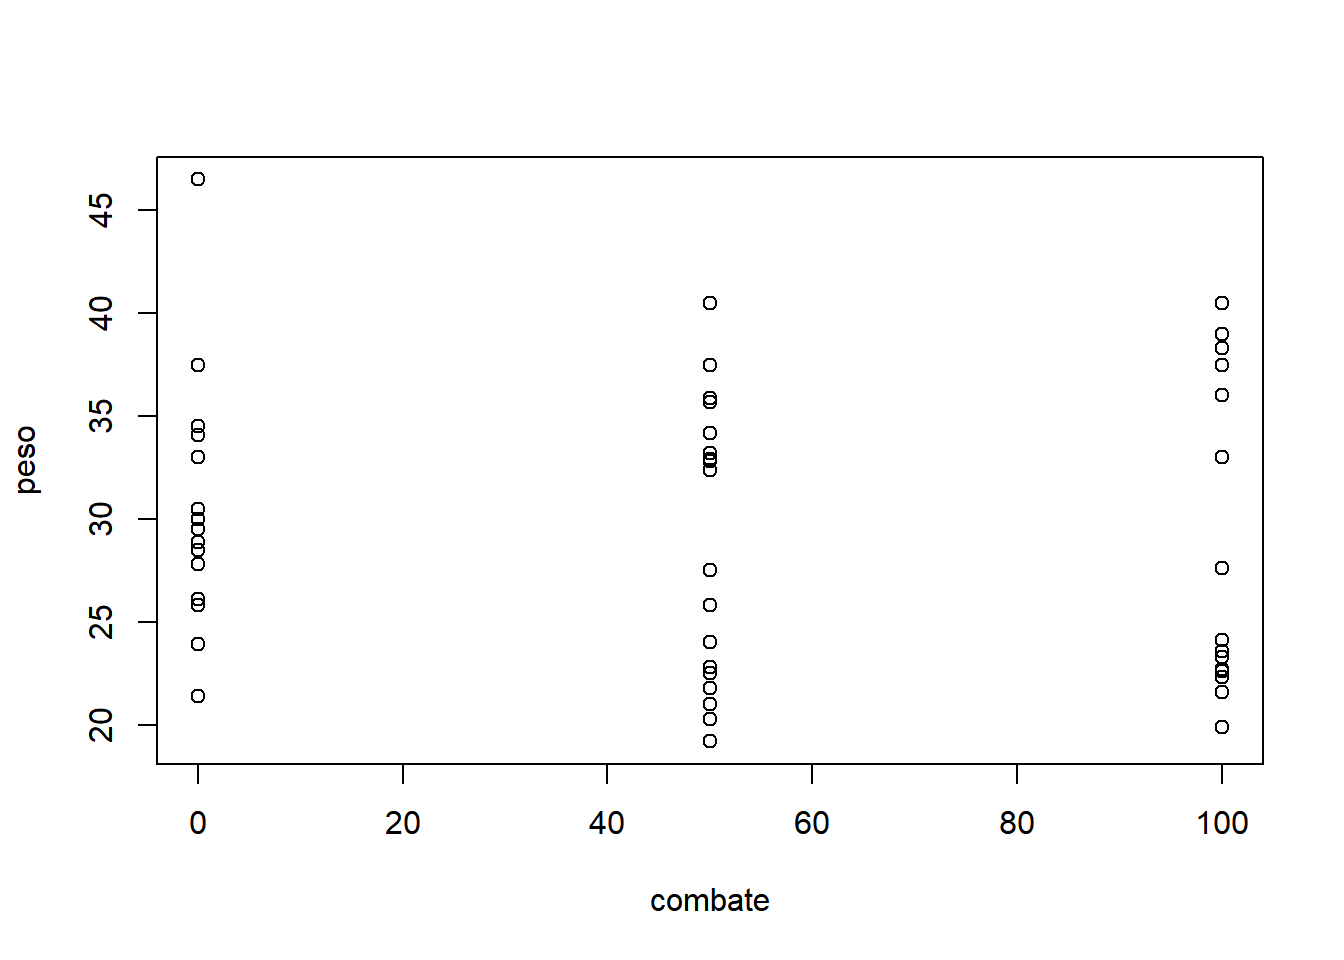
\includegraphics{bookdown_files/unnamed-chunk-126-1.png}

\begin{enumerate}
\def\labelenumi{\arabic{enumi}.}
\setcounter{enumi}{1}
\tightlist
\item
  Considerando apenas fator 2:
\end{enumerate}

\begin{Shaded}
\begin{Highlighting}[]
\KeywordTok{boxplot}\NormalTok{(}\DataTypeTok{data =}\NormalTok{ fatDBC2, peso }\OperatorTok{~}\StringTok{ }\NormalTok{especie)}
\end{Highlighting}
\end{Shaded}

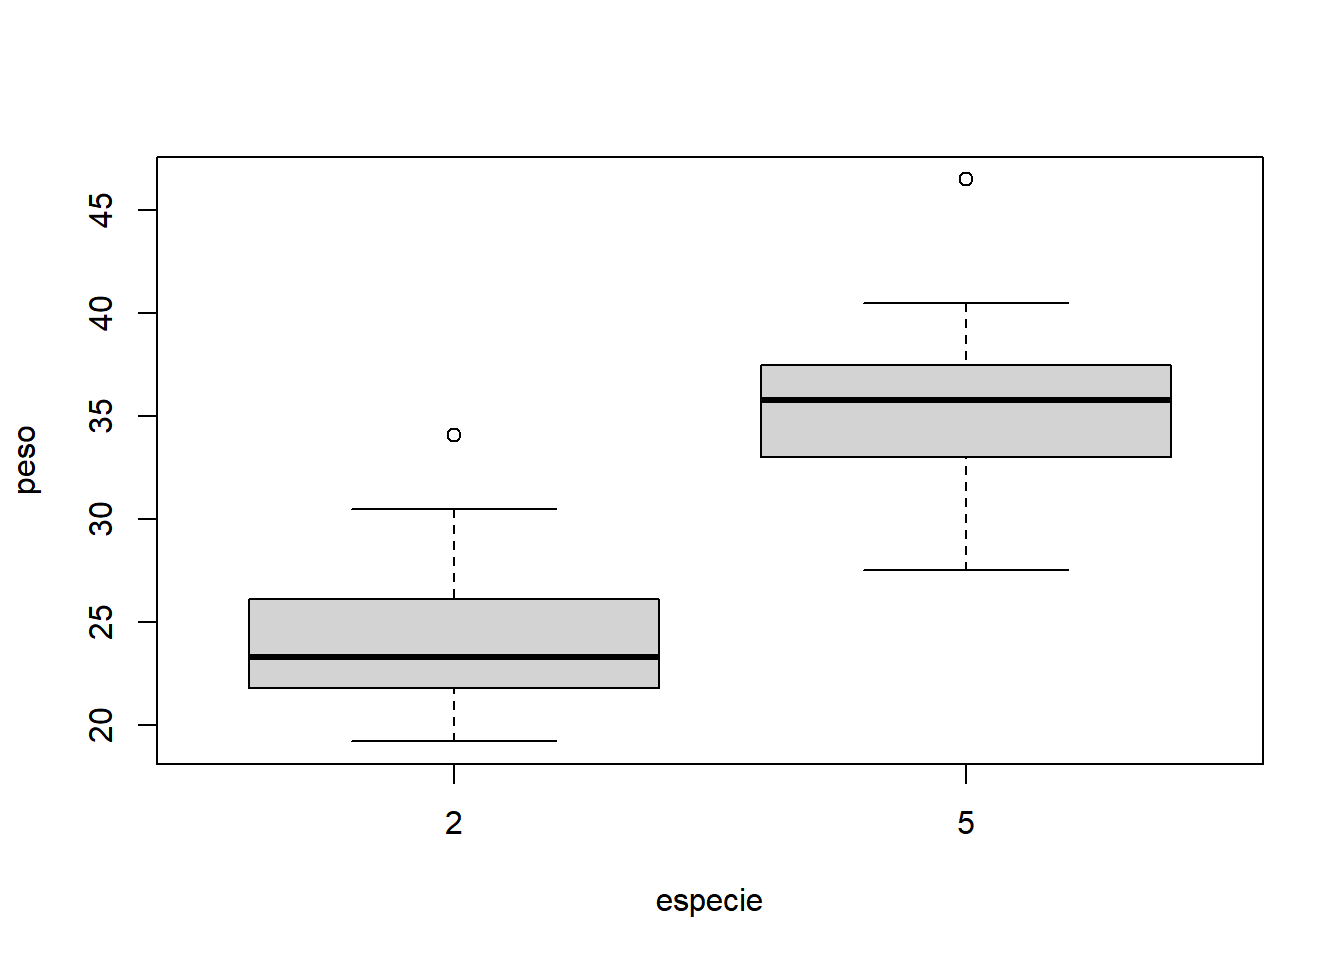
\includegraphics{bookdown_files/unnamed-chunk-127-1.png}

\begin{enumerate}
\def\labelenumi{\arabic{enumi}.}
\setcounter{enumi}{2}
\tightlist
\item
  Interação dos fatores:
\end{enumerate}

\begin{Shaded}
\begin{Highlighting}[]
\KeywordTok{boxplot}\NormalTok{(}\DataTypeTok{data =}\NormalTok{ fatDBC2, peso }\OperatorTok{~}\StringTok{ }\NormalTok{especie}\OperatorTok{/}\NormalTok{combate)}
\end{Highlighting}
\end{Shaded}

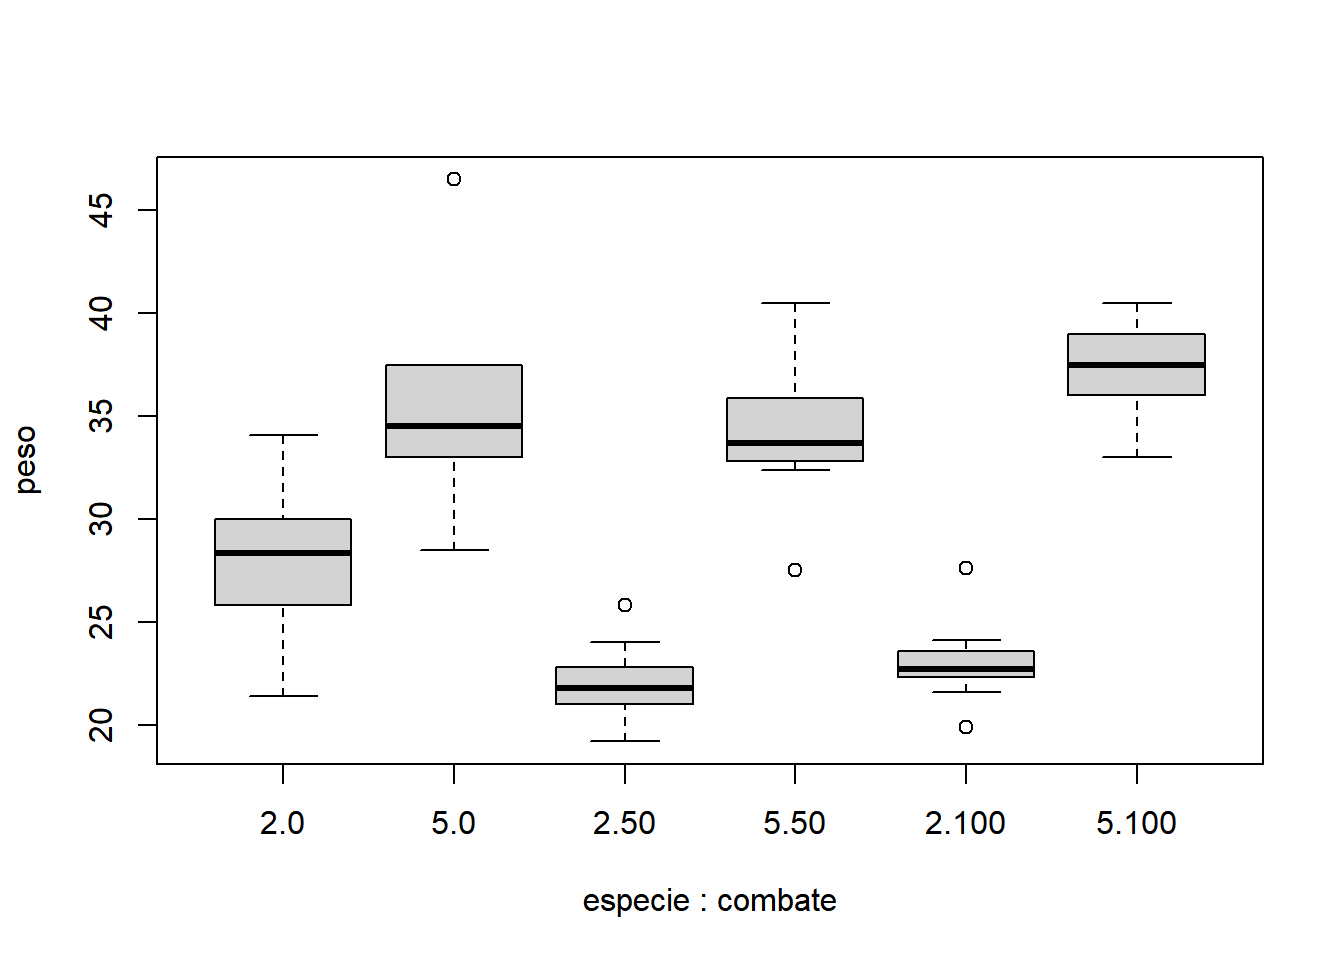
\includegraphics{bookdown_files/unnamed-chunk-128-1.png}

\begin{enumerate}
\def\labelenumi{\arabic{enumi}.}
\setcounter{enumi}{3}
\tightlist
\item
  Efeito dos blocos:
\end{enumerate}

\begin{Shaded}
\begin{Highlighting}[]
\KeywordTok{boxplot}\NormalTok{(}\DataTypeTok{data =}\NormalTok{ fatDBC2, peso }\OperatorTok{~}\StringTok{ }\NormalTok{especie}\OperatorTok{/}\NormalTok{bloco)}
\end{Highlighting}
\end{Shaded}

\includegraphics{bookdown_files/unnamed-chunk-129-1.png}

\begin{Shaded}
\begin{Highlighting}[]
\KeywordTok{boxplot}\NormalTok{(}\DataTypeTok{data =}\NormalTok{ fatDBC2, peso }\OperatorTok{~}\StringTok{ }\NormalTok{combate}\OperatorTok{/}\NormalTok{bloco)}
\end{Highlighting}
\end{Shaded}

\includegraphics{bookdown_files/unnamed-chunk-129-2.png}

\begin{enumerate}
\def\labelenumi{\arabic{enumi}.}
\setcounter{enumi}{4}
\tightlist
\item
  Fixando especie igual a 2:
\end{enumerate}

\begin{Shaded}
\begin{Highlighting}[]
\KeywordTok{plot}\NormalTok{(}\DataTypeTok{data =}\NormalTok{ fatDBC2[fatDBC2}\OperatorTok{$}\NormalTok{especie }\OperatorTok{==}\StringTok{ }\DecValTok{2}\NormalTok{,], peso }\OperatorTok{~}\StringTok{ }\NormalTok{combate)}
\end{Highlighting}
\end{Shaded}

\includegraphics{bookdown_files/unnamed-chunk-130-1.png}

\begin{enumerate}
\def\labelenumi{\arabic{enumi}.}
\setcounter{enumi}{5}
\tightlist
\item
  Fixando especie igual a 5:
\end{enumerate}

\begin{Shaded}
\begin{Highlighting}[]
\KeywordTok{plot}\NormalTok{(}\DataTypeTok{data =}\NormalTok{ fatDBC2[fatDBC2}\OperatorTok{$}\NormalTok{especie }\OperatorTok{==}\StringTok{ }\DecValTok{5}\NormalTok{,], peso }\OperatorTok{~}\StringTok{ }\NormalTok{combate)}
\end{Highlighting}
\end{Shaded}

\includegraphics{bookdown_files/unnamed-chunk-131-1.png}

\begin{enumerate}
\def\labelenumi{\arabic{enumi}.}
\setcounter{enumi}{6}
\tightlist
\item
  Fixando combate igual a 0:
\end{enumerate}

\begin{Shaded}
\begin{Highlighting}[]
\KeywordTok{boxplot}\NormalTok{(}\DataTypeTok{data =}\NormalTok{ fatDBC2[fatDBC2}\OperatorTok{$}\NormalTok{combate }\OperatorTok{==}\StringTok{ }\DecValTok{0}\NormalTok{,], peso }\OperatorTok{~}\StringTok{ }\NormalTok{especie)}
\end{Highlighting}
\end{Shaded}

\includegraphics{bookdown_files/unnamed-chunk-132-1.png}

\begin{enumerate}
\def\labelenumi{\arabic{enumi}.}
\setcounter{enumi}{7}
\tightlist
\item
  Fixando combate igual a 50:
\end{enumerate}

\begin{Shaded}
\begin{Highlighting}[]
\KeywordTok{boxplot}\NormalTok{(}\DataTypeTok{data =}\NormalTok{ fatDBC2[fatDBC2}\OperatorTok{$}\NormalTok{combate }\OperatorTok{==}\StringTok{ }\DecValTok{50}\NormalTok{,], peso }\OperatorTok{~}\StringTok{ }\NormalTok{especie)}
\end{Highlighting}
\end{Shaded}

\includegraphics{bookdown_files/unnamed-chunk-133-1.png}

\begin{enumerate}
\def\labelenumi{\arabic{enumi}.}
\setcounter{enumi}{8}
\tightlist
\item
  Fixando combate igual a 100:
\end{enumerate}

\begin{Shaded}
\begin{Highlighting}[]
\KeywordTok{boxplot}\NormalTok{(}\DataTypeTok{data =}\NormalTok{ fatDBC2[fatDBC2}\OperatorTok{$}\NormalTok{combate }\OperatorTok{==}\StringTok{ }\DecValTok{100}\NormalTok{,], peso }\OperatorTok{~}\StringTok{ }\NormalTok{especie)}
\end{Highlighting}
\end{Shaded}

\includegraphics{bookdown_files/unnamed-chunk-134-1.png}

Como o delineamento fatorial duplo em blocos casualizados pode ter a interação significativa, é fundamental considerar a análise através da ANOVA tipo III. A sintaxe da função é:

\begin{Shaded}
\begin{Highlighting}[]
\KeywordTok{ea2}\NormalTok{(data, }\DataTypeTok{design =} \DecValTok{1}\NormalTok{, }\DataTypeTok{alpha =} \FloatTok{0.05}\NormalTok{, }\DataTypeTok{cov =} \DecValTok{4}\NormalTok{, }\DataTypeTok{list =} \OtherTok{FALSE}\NormalTok{, }
    \DataTypeTok{p.adjust=}\DecValTok{1}\NormalTok{,}\DataTypeTok{plot=}\DecValTok{2}\NormalTok{)}
\end{Highlighting}
\end{Shaded}

Como já mencionado, o pacote \texttt{easyanova} exige que os dados sejam apresentados em forma de dataframe contendo apenas as colunas relevantes para a análise. No caso de um experimento fatorial duplo em blocos casualizados, a ordem esperada das colunas é:

\begin{enumerate}
\def\labelenumi{\arabic{enumi}.}
\tightlist
\item
  Fator A
\item
  Fator B
\item
  Bloco
\item
  Variável resposta
\end{enumerate}

Qualquer variável extra deve ser removida dos dados e a ordem acima deve ser respeitada para o correto uso do pacote. Além de apresentar os dados na estrutura correta, o parâmetro \texttt{design} deve ser ajustado para \texttt{2}, indicando fatorial duplo em blocos casualizados.

\begin{Shaded}
\begin{Highlighting}[]
\KeywordTok{require}\NormalTok{(easyanova)}
\NormalTok{r.aov =}\StringTok{ }\KeywordTok{ea2}\NormalTok{(fatDBC2, }\DataTypeTok{design =} \DecValTok{2}\NormalTok{)}
\end{Highlighting}
\end{Shaded}

\includegraphics{bookdown_files/unnamed-chunk-136-1.png}

Os resultados são armazenados numa lista de 10 posições, aqui salva numa variável denominada de \texttt{r.aov}. As 10 posições contém:

\begin{enumerate}
\def\labelenumi{\arabic{enumi}.}
\tightlist
\item
  Análise de variância
\item
  Comparação de médias do fator 1
\item
  Teste de comparação múltipla do fator 1
\item
  Comparação de médias do fator 2
\item
  Teste de comparação múltipla do fator 2
\item
  Comparação de médias do fator 1 dentro dos níveis do fator 2
\item
  Teste de comparação múltipla do fator 1 dentro dos níveis do fator 2
\item
  Comparação de médias do fator 2 dentro dos níveis do fator 1
\item
  Teste de comparação múltipla do fator 2 dentro dos níveis do fator 1
\item
  Análise das pressuposições
\end{enumerate}

Nota-se que o teste de Shapiro-Wilk não é significativo, aceitando-se portanto o teste de nulidade, e portanto de resíduos normais.

\begin{Shaded}
\begin{Highlighting}[]
\NormalTok{r.aov[}\DecValTok{10}\NormalTok{]}
\end{Highlighting}
\end{Shaded}

\begin{verbatim}
## $`Residual analysis`
## $`Residual analysis`$`residual analysis`
##                                     values
## p.value Shapiro-Wilk test           0.0847
## p.value Bartlett test (factor_1)    0.0888
## p.value Bartlett test (factor_2)    0.1543
## p.value Bartlett test (treatments)  0.2051
## coefficient of variation (%)       10.8100
## first value most discrepant        59.0000
## second value most discrepant       46.0000
## third value most discrepant        25.0000
## 
## $`Residual analysis`$residuals
##          1          2          3          4 
## -1.0666667  0.2666667  3.7333333 -1.1666667 
##          5          6          7          8 
##  0.4166667 -2.9000000  0.6333333  2.9166667 
##          9         10         11         12 
## -2.8333333  0.8853333  0.5186667 -1.0146667 
##         13         14         15         16 
##  3.3853333 -0.8313333  2.2520000 -1.8146667 
##         17         18         19         20 
## -1.6680000  1.6686667 -3.3813333  2.6053333 
##         21         22         23         24 
## -2.2613333 -0.7946667 -2.0946667  0.4886667 
##         25         26         27         28 
##  6.5720000 -2.8946667  1.7520000 -3.7113333 
##         29         30         31         32 
##  0.3386667 -1.1746667  2.6586667 -0.8746667 
##         33         34         35         36 
## -4.9746667  0.1086667  0.1920000  0.9253333 
##         37         38         39         40 
##  1.4720000  1.1086667  0.5586667 -1.0546667 
##         41         42         43         44 
##  1.1786667 -2.6546667  2.8453333  1.0286667 
##         45         46         47         48 
##  0.2120000  7.2453333 -1.0080000 -4.0713333 
##         49         50         51         52 
## -3.7213333 -0.1946667 -2.3613333  1.6053333 
##         53         54         55         56 
##  2.0053333 -1.2113333 -6.3280000 -4.0946667 
##         57         58         59 
## -0.5480000  2.0886667  9.0386667 
## 
## $`Residual analysis`$`standardized residuals`
##           1           2           3           4 
## -0.37654793  0.09413698  1.31791775 -0.41184930 
##           5           6           7           8 
##  0.14708903 -1.02373968  0.22357533  1.02962324 
##           9          10          11          12 
## -1.00020543  0.31253478  0.18309643 -0.35819122 
##          13          14          15          16 
##  1.19506899 -0.29347204  0.79498681 -0.64060216 
##          17          18          19          20 
## -0.58882682  0.58906216 -1.19365693  0.91971831 
##          21          22          23          24 
## -0.79828161 -0.28052821 -0.73944599  0.17250602 
##          25          26          27          28 
##  2.32000592 -1.02185694  0.61847997 -1.31015145 
##          29          30          31          32 
##  0.11955397 -0.41467341  0.93854571 -0.30876930 
##          33          34          35          36 
## -1.75612540  0.03836082  0.06777863  0.32665533 
##          37          38          39          40 
##  0.51963614  0.39137450  0.19721698 -0.37231176 
##          41          42          43          44 
##  0.41608546 -0.93713365  1.00444160  0.36313341 
##          45          46          47          48 
##  0.07483890  2.55770180 -0.35583779 -1.43723637 
##          49          50          51          52 
## -1.31368158 -0.06872000 -0.83358297  0.56670463 
##          53          54          55          56 
##  0.70791010 -0.42761724 -2.23387058 -1.44547336 
##          57          58          59 
## -0.19345150  0.73732791  3.19077300
\end{verbatim}

O quadro geral da ANOVA indica que os dois fatores, bem como a interação são significativos:

\begin{Shaded}
\begin{Highlighting}[]
\NormalTok{r.aov[}\DecValTok{1}\NormalTok{]}
\end{Highlighting}
\end{Shaded}

\begin{verbatim}
## $`Analysis of variance`
##                   df type III SS mean square
## factor_1           2    113.1605     56.5803
## factor_2           1   1890.1081   1890.1081
## blocks             9     91.7117     10.1902
## factor_1:factor_2  2    132.6536     66.3268
## residuals         44    465.4199     10.5777
##                    F value    p>F
## factor_1             5.349 0.0083
## factor_2          178.6876 <0.001
## blocks              0.9634 0.4825
## factor_1:factor_2   6.2704  0.004
## residuals                -      -
\end{verbatim}

Parte-se direto, portanto, para a análise dos respectivos desdobramentos presentes nas posições 6 e 8 da lista de resultados (\texttt{r.aov{[}6{]}} e \texttt{r.aov{[}8{]}}):

\begin{enumerate}
\def\labelenumi{\arabic{enumi}.}
\tightlist
\item
  Comparação de médias do fator 1 dentro do fator 2:
\end{enumerate}

\begin{Shaded}
\begin{Highlighting}[]
\NormalTok{r.aov[}\DecValTok{6}\NormalTok{]}
\end{Highlighting}
\end{Shaded}

\begin{verbatim}
## $`Adjusted means (factor 1 in levels of factor 2)`
## $`Adjusted means (factor 1 in levels of factor 2)`$`factor_1 in  2`
##   treatment adjusted.mean standard.error tukey snk
## 1       0.2        27.800         1.0285     a   a
## 3     100.2        23.072         1.0285     b   b
## 2      50.2        22.020         1.0285     b   b
##   duncan t scott_knott
## 1      a a           a
## 3      b b           b
## 2      b b           b
## 
## $`Adjusted means (factor 1 in levels of factor 2)`$`factor_1 in  5`
##   treatment adjusted.mean standard.error tukey snk
## 6     100.5         37.58         1.0285     a   a
## 4       0.5         35.10         1.0285     a   a
## 5      50.5         34.26         1.0285     a   a
##   duncan  t scott_knott
## 6      a  a           a
## 4     ab ab           a
## 5      b  b           a
\end{verbatim}

\begin{enumerate}
\def\labelenumi{\arabic{enumi}.}
\setcounter{enumi}{1}
\tightlist
\item
  Comparação de médias do fator 2 dentro do fator 1:
\end{enumerate}

\begin{Shaded}
\begin{Highlighting}[]
\NormalTok{r.aov[}\DecValTok{8}\NormalTok{]}
\end{Highlighting}
\end{Shaded}

\begin{verbatim}
## $`Adjusted means (factor 2 in levels of factor 1)`
## $`Adjusted means (factor 2 in levels of factor 1)`$`factor_2 in  0`
##   treatment adjusted.mean standard.error tukey snk
## 4       0.5          35.1         1.0285     a   a
## 1       0.2          27.8         1.0285     b   b
##   duncan t scott_knott
## 4      a a           a
## 1      b b           b
## 
## $`Adjusted means (factor 2 in levels of factor 1)`$`factor_2 in  50`
##   treatment adjusted.mean standard.error tukey snk
## 5      50.5         34.26         1.0285     a   a
## 2      50.2         22.02         1.0285     b   b
##   duncan t scott_knott
## 5      a a           a
## 2      b b           b
## 
## $`Adjusted means (factor 2 in levels of factor 1)`$`factor_2 in  100`
##   treatment adjusted.mean standard.error tukey snk
## 6     100.5        37.580         1.0285     a   a
## 3     100.2        23.072         1.0285     b   b
##   duncan t scott_knott
## 6      a a           a
## 3      b b           b
\end{verbatim}

Fique atento! O pacote \texttt{easyanova} não diferencia fatores qualitativos e quantitativos, analisando todos os fatores e seus desdobramentos com teste comparativo de média.

\hypertarget{parcela-subdividida}{%
\section{Parcela subdividida}\label{parcela-subdividida}}

No delineamento em parcelas subdivididas existem dois tipos de tratamento: o principal e o secundário. As parcelas são subdivididas no espaço, ou no tempo. Depois que os tratamentos principais (parcelas) são sorteados, sorteia-se o tratamento secundário (subparcelas) dentro das parcelas.

Indica-se o uso de parcelas subdivididas quando:

\begin{enumerate}
\def\labelenumi{\arabic{enumi}.}
\tightlist
\item
  A parcela é uma ``unidade'' que pode receber vários tratamentos secundários. No setor florestal esta unidade pode ser um vaso, ou mesmo uma árvore.
\item
  Não é possível instalar o experimento no esquema fatorial.
\item
  O tratamento principal exige parcelas custosas, seja do ponto de vista financeiro ou do esforço.
\item
  A busca pela precisão está no tratamento secundário.
\item
  Deseja-se que a variação entre subparcelas seja menor que entre as parcelas.
\end{enumerate}

O modelo estatístico do delineamento em parcela subdividida é:

\[Y = \bar{Y} + BLOCO + TRAT_A + Erro_{Parcela} + TRAT_B + (TRAT_A * TRAT_B) + Erro_{Subparcela}\]

\hypertarget{o-caso-balanceado-4}{%
\subsection{O caso balanceado}\label{o-caso-balanceado-4}}

Como exemplo de um desenho de parcela subdividida balanceado, tem-se um experimento de regeneração natural do sub bosque de três formações florestais. Nas parcelas de cada uma das área naturais estudadas, implantaram-se subparcelas correspondendo a três alturas de desrama. O efeito dos tratamentos foi medido através do número de indivíduos regenerantes.

\begin{itemize}
\tightlist
\item
  Fator na parcela: Floresta A, B e C
\item
  Fator nas subparcelas: Desrama a 2, 5 e 7 metros
\item
  3 repetições
\item
  Variável de interesse: número de indivíduos regenerantes
\end{itemize}

\begin{table}

\caption{\label{tab:unnamed-chunk-141}Dados de experimento em parcela subdividida}
\centering
\begin{tabular}[t]{l|r|r|r}
\hline
floresta & rep & desrama & indiv\\
\hline
A & 1 & 2 & 48\\
\hline
A & 2 & 2 & 47\\
\hline
A & 3 & 2 & 47\\
\hline
A & 1 & 5 & 79\\
\hline
A & 2 & 5 & 62\\
\hline
A & 3 & 5 & 65\\
\hline
A & 1 & 7 & 101\\
\hline
A & 2 & 7 & 105\\
\hline
A & 3 & 7 & 112\\
\hline
B & 1 & 2 & 90\\
\hline
B & 2 & 2 & 97\\
\hline
B & 3 & 2 & 114\\
\hline
B & 1 & 5 & 123\\
\hline
B & 2 & 5 & 145\\
\hline
B & 3 & 5 & 122\\
\hline
B & 1 & 7 & 172\\
\hline
B & 2 & 7 & 157\\
\hline
B & 3 & 7 & 177\\
\hline
C & 1 & 2 & 100\\
\hline
C & 2 & 2 & 101\\
\hline
C & 3 & 2 & 103\\
\hline
C & 1 & 5 & 130\\
\hline
C & 2 & 5 & 133\\
\hline
C & 3 & 5 & 140\\
\hline
C & 1 & 7 & 144\\
\hline
C & 2 & 7 & 147\\
\hline
C & 3 & 7 & 148\\
\hline
\end{tabular}
\end{table}

O primeiro passo é importar o arquivo contendo os resultados do experimento para dentro do R. Esta tarefa pode ser realizada através do seguinte comando:

\begin{Shaded}
\begin{Highlighting}[]
\NormalTok{sub =}\StringTok{ }\KeywordTok{read.csv}\NormalTok{(}\StringTok{"./data/Experimento Subdividida.csv"}\NormalTok{, }
               \DataTypeTok{sep =} \StringTok{","}\NormalTok{, }\DataTypeTok{dec =} \StringTok{"."}\NormalTok{)}
\end{Highlighting}
\end{Shaded}

Você já sabe! Antes de ir para análise estatística explore graficamente os dados.

\begin{enumerate}
\def\labelenumi{\arabic{enumi}.}
\tightlist
\item
  Considerando apenas tratamento principal:
\end{enumerate}

\begin{Shaded}
\begin{Highlighting}[]
\KeywordTok{boxplot}\NormalTok{(}\DataTypeTok{data =}\NormalTok{ sub, indiv }\OperatorTok{~}\StringTok{ }\NormalTok{floresta)}
\end{Highlighting}
\end{Shaded}

\includegraphics{bookdown_files/unnamed-chunk-143-1.png}

\begin{enumerate}
\def\labelenumi{\arabic{enumi}.}
\setcounter{enumi}{1}
\tightlist
\item
  Considerando apenas tratamento secundário:
\end{enumerate}

\begin{Shaded}
\begin{Highlighting}[]
\KeywordTok{plot}\NormalTok{(}\DataTypeTok{data =}\NormalTok{ sub, indiv }\OperatorTok{~}\StringTok{ }\NormalTok{desrama)}
\end{Highlighting}
\end{Shaded}

\includegraphics{bookdown_files/unnamed-chunk-144-1.png}

\begin{enumerate}
\def\labelenumi{\arabic{enumi}.}
\setcounter{enumi}{2}
\tightlist
\item
  Interação dos tratamentos:
\end{enumerate}

\begin{Shaded}
\begin{Highlighting}[]
\KeywordTok{boxplot}\NormalTok{(}\DataTypeTok{data =}\NormalTok{ sub, indiv }\OperatorTok{~}\StringTok{ }\NormalTok{floresta}\OperatorTok{/}\NormalTok{desrama)}
\end{Highlighting}
\end{Shaded}

\includegraphics{bookdown_files/unnamed-chunk-145-1.png}

\begin{enumerate}
\def\labelenumi{\arabic{enumi}.}
\setcounter{enumi}{3}
\tightlist
\item
  Fixando desrana até 2 metros:
\end{enumerate}

\begin{Shaded}
\begin{Highlighting}[]
\KeywordTok{boxplot}\NormalTok{(}\DataTypeTok{data =}\NormalTok{ sub[sub}\OperatorTok{$}\NormalTok{desrama }\OperatorTok{==}\StringTok{ }\DecValTok{2}\NormalTok{,], indiv }\OperatorTok{~}\StringTok{ }\NormalTok{floresta)}
\end{Highlighting}
\end{Shaded}

\includegraphics{bookdown_files/unnamed-chunk-146-1.png}

\begin{enumerate}
\def\labelenumi{\arabic{enumi}.}
\setcounter{enumi}{4}
\tightlist
\item
  Fixando desrana até 5 metros:
\end{enumerate}

\begin{Shaded}
\begin{Highlighting}[]
\KeywordTok{boxplot}\NormalTok{(}\DataTypeTok{data =}\NormalTok{ sub[sub}\OperatorTok{$}\NormalTok{desrama }\OperatorTok{==}\StringTok{ }\DecValTok{5}\NormalTok{,], indiv }\OperatorTok{~}\StringTok{ }\NormalTok{floresta)}
\end{Highlighting}
\end{Shaded}

\includegraphics{bookdown_files/unnamed-chunk-147-1.png}

\begin{enumerate}
\def\labelenumi{\arabic{enumi}.}
\setcounter{enumi}{5}
\tightlist
\item
  Fixando desrana até 7 metros:
\end{enumerate}

\begin{Shaded}
\begin{Highlighting}[]
\KeywordTok{boxplot}\NormalTok{(}\DataTypeTok{data =}\NormalTok{ sub[sub}\OperatorTok{$}\NormalTok{desrama }\OperatorTok{==}\StringTok{ }\DecValTok{7}\NormalTok{,], indiv }\OperatorTok{~}\StringTok{ }\NormalTok{floresta)}
\end{Highlighting}
\end{Shaded}

\includegraphics{bookdown_files/unnamed-chunk-148-1.png}

\begin{enumerate}
\def\labelenumi{\arabic{enumi}.}
\setcounter{enumi}{6}
\tightlist
\item
  Fixando floresta igual a A:
\end{enumerate}

\begin{Shaded}
\begin{Highlighting}[]
\KeywordTok{plot}\NormalTok{(}\DataTypeTok{data =}\NormalTok{ sub[sub}\OperatorTok{$}\NormalTok{floresta }\OperatorTok{==}\StringTok{ "A"}\NormalTok{,], indiv }\OperatorTok{~}\StringTok{ }\NormalTok{desrama)}
\end{Highlighting}
\end{Shaded}

\includegraphics{bookdown_files/unnamed-chunk-149-1.png}

\begin{enumerate}
\def\labelenumi{\arabic{enumi}.}
\setcounter{enumi}{7}
\tightlist
\item
  Fixando floresta igual a B:
\end{enumerate}

\begin{Shaded}
\begin{Highlighting}[]
\KeywordTok{plot}\NormalTok{(}\DataTypeTok{data =}\NormalTok{ sub[sub}\OperatorTok{$}\NormalTok{floresta }\OperatorTok{==}\StringTok{ "B"}\NormalTok{,], indiv }\OperatorTok{~}\StringTok{ }\NormalTok{desrama)}
\end{Highlighting}
\end{Shaded}

\includegraphics{bookdown_files/unnamed-chunk-150-1.png}

\begin{enumerate}
\def\labelenumi{\arabic{enumi}.}
\setcounter{enumi}{8}
\tightlist
\item
  Fixando floresta igual a C:
\end{enumerate}

\begin{Shaded}
\begin{Highlighting}[]
\KeywordTok{plot}\NormalTok{(}\DataTypeTok{data =}\NormalTok{ sub[sub}\OperatorTok{$}\NormalTok{floresta }\OperatorTok{==}\StringTok{ "C"}\NormalTok{,], indiv }\OperatorTok{~}\StringTok{ }\NormalTok{desrama)}
\end{Highlighting}
\end{Shaded}

\includegraphics{bookdown_files/unnamed-chunk-151-1.png}

Analisando os gráficos acima, os fatores parecem significativos, assim como a interação. Quando o interesse é verificar a questão das pressuposições considerando os tratamentos (Parcela e Subparcela juntos), além das colunas referentes a parcela e subparcela, teria que ser acrescentado uma coluna para tratamentos. Ou seja, é como se fosse uma análise preliminar como DIC ou DBC.

O pacote \texttt{ExpDes.pt} não inclui as análises de pressuposições para o delineamento de parcelas subdivididas. Existem várias maneiras de contornar esta questão, uma delas é combinar as qualidades de diferentes pacotes. Aqui por exemplo, utiliza-se os testes estatísticos das pressuposições de um pacote e a ANOVA e desdobramentos do outro.

\begin{Shaded}
\begin{Highlighting}[]
\KeywordTok{require}\NormalTok{(easyanova)}
\NormalTok{r.aov =}\StringTok{ }\KeywordTok{ea2}\NormalTok{(sub, }\DataTypeTok{design=}\DecValTok{4}\NormalTok{)}
\end{Highlighting}
\end{Shaded}

\includegraphics{bookdown_files/unnamed-chunk-152-1.png}

Como já foi visto, o teste de normalidade e de homogeneidade podem ser obtidos na posição 10 da função \texttt{ea2()} do pacote \texttt{easyanova}.

\begin{Shaded}
\begin{Highlighting}[]
\NormalTok{r.aov[}\DecValTok{10}\NormalTok{]}
\end{Highlighting}
\end{Shaded}

\begin{verbatim}
## $`Residual analysis`
## $`Residual analysis`$values
##                                           values
## p.value Shapiro-Wilk test                 0.4583
## p.value Bartlett test (plot)              0.0036
## p.value Bartlett test (split.plot)        0.5945
## p.value Bartlett test (plot*split.plot)   0.0264
## AIC                                     171.9126
## BIC                                     182.5971
## first value most discrepant              14.0000
## second value most discrepant             12.0000
## third value most discrepant              17.0000
## Mean Square of Error a                   35.6667
## Mean Square of Error b                   64.0009
## Coefficient of Variation a                5.3589
## Coefficient of Variation b                7.1785
## 
## $`Residual analysis`$residuals
##           1           2           3           4 
##   0.6605916  -0.3252332  -0.3353584  10.3272582 
##           5           6           7           8 
##  -6.6585666  -3.6686917  -5.0060751  -0.9918999 
##           9          10          11          12 
##   5.9979750 -10.3191581  -3.3333333  13.6524915 
##          13          14          15          16 
##  -6.9858248  15.0000000  -8.0141752   3.3475085 
##          17          18          19          20 
## -11.6666667   8.3191581  -1.3252332  -0.3323208 
##          21          22          23          24 
##   1.6575540  -4.3252332  -1.3323208   5.6575540 
##          25          26          27 
##  -2.3252332   0.6676792   1.6575540 
## attr(,"label")
## [1] "Residuals"
## 
## $`Residual analysis`$`standardized residuals`
##           1           2           3           4 
##  0.09926874 -0.04887361 -0.05039514  1.55190283 
##           5           6           7           8 
## -1.00059939 -0.55130344 -0.75227538 -0.14905527 
##           9          10          11          12 
##  0.90133065 -1.55068561 -0.50090831  2.05159391 
##          13          14          15          16 
## -1.04977730  2.25408738 -1.20431008  0.50303845 
##          17          18          19          20 
## -1.75317907  1.25014062 -0.19914610 -0.04993868 
##          21          22          23          24 
##  0.24908478 -0.64996357 -0.20021117  0.85017474 
##          25          26          27 
## -0.34941859  0.10033381  0.24908478
\end{verbatim}

Uma vez confirmadas as pressuposições, retorna-se ao pacote \texttt{ExpDes.pt}. A sintaxe da função para análise de parcela subdividida no pacote é:

\begin{Shaded}
\begin{Highlighting}[]
\KeywordTok{psub2.dic}\NormalTok{(fator1, fator2, repet, resp, }\DataTypeTok{quali =} \KeywordTok{c}\NormalTok{(}\OtherTok{TRUE}\NormalTok{, }\OtherTok{TRUE}\NormalTok{),}
          \DataTypeTok{mcomp =} \StringTok{"tukey"}\NormalTok{, }\DataTypeTok{fac.names =} \KeywordTok{c}\NormalTok{(}\StringTok{"F1"}\NormalTok{, }\StringTok{"F2"}\NormalTok{), }
          \DataTypeTok{sigT =} \FloatTok{0.05}\NormalTok{, }\DataTypeTok{sigF =} \FloatTok{0.05}\NormalTok{)}
\end{Highlighting}
\end{Shaded}

No exemplo tem-se o fator principal (fator 1) como qualitativo e o fator secundário (fator 2) como quantitativo. Assim informando os parâmetros obrigatórios juntamente com os parâmetros \texttt{quali} e \texttt{fac.names} (nomes dos fatores) tem-se:

\begin{Shaded}
\begin{Highlighting}[]
\KeywordTok{require}\NormalTok{(ExpDes.pt)}
\KeywordTok{psub2.dic}\NormalTok{(sub}\OperatorTok{$}\NormalTok{floresta, sub}\OperatorTok{$}\NormalTok{desrama, sub}\OperatorTok{$}\NormalTok{rep, sub}\OperatorTok{$}\NormalTok{indiv,}
          \DataTypeTok{quali =} \KeywordTok{c}\NormalTok{(}\OtherTok{TRUE}\NormalTok{, }\OtherTok{FALSE}\NormalTok{), }
          \DataTypeTok{fac.names =} \KeywordTok{c}\NormalTok{(}\StringTok{"Floresta"}\NormalTok{, }\StringTok{"Desrama"}\NormalTok{))}
\end{Highlighting}
\end{Shaded}

\begin{verbatim}
## ------------------------------------------------------------------------
## Legenda:
## FATOR 1    (parcela):  Floresta 
## FATOR 2 (subparcela):  Desrama 
## ------------------------------------------------------------------------
## 
## ------------------------------------------------------------------------
## $`Quadro da analise de variancia`
##                  GL    SQ     QM      Fc Pr(>Fc)
## Floresta          2 19073 9536.3 267.374   1e-06
## Erro a            6   214   35.7                
## Desrama           2 14795 7397.3  94.568 < 2e-16
## Floresta*Desrama  4   799  199.7   2.553 0.09349
## Erro b           12   939   78.2                
## Total            26 35819                       
##                     
## Floresta         ***
## Erro a              
## Desrama          ***
## Floresta*Desrama .  
## Erro b              
## Total               
## ---
## Signif. codes:  
## 0 '***' 0.001 '**' 0.01 '*' 0.05 '.' 0.1 ' ' 1
## 
## ------------------------------------------------------------------------
## CV 1 = 5.358865 %
## CV 2 = 7.936091 %
## 
## ------------------------------------------------------------------------
## #Teste de normalidade dos residuos (Shapiro-Wilk)
## valor-p:  0.5769146 
## De acordo com o teste de Shapiro-Wilk a 5% de significancia, os residuos podem ser considerados normais.
## ------------------------------------------------------------------------
## 
## Interacao nao significativa: analisando os efeitos simples
## ------------------------------------------------------------------------
## Floresta
## Teste de Tukey
## ------------------------------------------------------------------------
## Grupos Tratamentos Medias
## a     B   133 
## a     C   127.3333 
##  b    A   74 
## ------------------------------------------------------------------------
## 
## Desrama
## Ajuste de modelos polinomiais de regressao
## ------------------------------------------------------------------------
## 
## Modelo Linear
## =========================================
##    Estimativa Erro.padrao   tc    valor.p
## -----------------------------------------
## b0  58.7193     4.2238    13.9021    0   
## b1  11.2982     0.8284    13.6395    0   
## -----------------------------------------
## 
## R2 do modelo linear
## --------
## 0.983607
## --------
## 
## Analise de variancia do modelo linear
## ==============================================================
##                      GL     SQ          QM        Fc   valor.p
## --------------------------------------------------------------
## Efeito linear        1  14,552.1400 14,552.1400 186.04    0   
## Desvios de Regressao 1   242.5263    242.5263    3.1   0.10371
## Residuos             12  938.6667     78.2222                 
## --------------------------------------------------------------
## ------------------------------------------------------------------------
## 
## Modelo quadratico
## ========================================
##    Estimativa Erro.padrao   tc   valor.p
## ----------------------------------------
## b0     75       10.1652   7.3781 0.00001
## b1   1.8667     5.4200    0.3444 0.7365 
## b2   1.0667     0.6058    1.7608 0.1037 
## ----------------------------------------
## 
## R2 do modelo quadratico
## -
## 1
## -
## 
## Analise de variancia do modelo quadratico
## ==============================================================
##                      GL     SQ          QM        Fc   valor.p
## --------------------------------------------------------------
## Efeito linear        1  14,552.1400 14,552.1400 186.04    0   
## Efeito quadratico    1   242.5263    242.5263    3.1   0.10371
## Desvios de Regressao 0       0           0        0       1   
## Residuos             12  938.6667     78.2222                 
## --------------------------------------------------------------
## ------------------------------------------------------------------------
\end{verbatim}

Como esperado, foi observado a significância dos fatores: floresta e desrama. No entanto, a interação não foi significativa a 5\%. Desta forma, não é necessário analisar a interação entre os fatores.

\hypertarget{o-caso-desbalanceado-4}{%
\subsection{O caso desbalanceado}\label{o-caso-desbalanceado-4}}

Neste exemplo desbalanceado será analisado um experimento em que três alturas de desrama são subdivididos em três espécies florestais. O efeito dos tratamentos foi medido através da produção de madeira em metros cúbicos.

\begin{itemize}
\tightlist
\item
  Fator na parcela: Espécie florestal: A, B ou C.
\item
  Fator nas subparcelas: Desrama 2, 5 e 7 metros.
\item
  3 repetições.
\item
  Observações perdidas: Espécie A, desrama 2 metros e repetição 2. Espécie C, desrama 2 metros e repetição 2. Espécie C, desrama 5 metros e repetição 1. Espécie C, desrama 7 metros e repetição 1.
\item
  Variável de interesse: número de indivíduos regenerantes.
\end{itemize}

\begin{table}

\caption{\label{tab:unnamed-chunk-156}Dados de outro experimento em parcela subdividida, porém desbalanceado.}
\centering
\begin{tabular}[t]{l|r|r|r}
\hline
especie & rep & desrama & volume\\
\hline
A & 1 & 2 & 48\\
\hline
A & 3 & 2 & 47\\
\hline
A & 1 & 5 & 79\\
\hline
A & 2 & 5 & 62\\
\hline
A & 3 & 5 & 65\\
\hline
A & 1 & 7 & 131\\
\hline
A & 2 & 7 & 65\\
\hline
A & 3 & 7 & 112\\
\hline
B & 1 & 2 & 80\\
\hline
B & 2 & 2 & 97\\
\hline
B & 3 & 2 & 114\\
\hline
B & 1 & 5 & 123\\
\hline
B & 2 & 5 & 145\\
\hline
B & 3 & 5 & 122\\
\hline
B & 1 & 7 & 172\\
\hline
B & 2 & 7 & 157\\
\hline
B & 3 & 7 & 177\\
\hline
C & 1 & 2 & 100\\
\hline
C & 3 & 2 & 103\\
\hline
C & 2 & 5 & 133\\
\hline
C & 3 & 5 & 104\\
\hline
C & 2 & 7 & 147\\
\hline
C & 3 & 7 & 119\\
\hline
\end{tabular}
\end{table}

O primeiro passo é importar o arquivo contendo os resultados do experimento para dentro do R. Esta tarefa pode ser realizada através do seguinte comando:

\begin{Shaded}
\begin{Highlighting}[]
\NormalTok{sub2 =}\StringTok{ }\KeywordTok{read.csv}\NormalTok{(}\StringTok{"./data/Experimento Subdividida 2.csv"}\NormalTok{, }\DataTypeTok{sep =} \StringTok{","}\NormalTok{, }\DataTypeTok{dec =} \StringTok{"."}\NormalTok{)}
\end{Highlighting}
\end{Shaded}

Os dados devem ser explorados graficamente antes de seguir com a análise de variância do experimento.

\begin{enumerate}
\def\labelenumi{\arabic{enumi}.}
\tightlist
\item
  Considerando apenas tratamento principal:
\end{enumerate}

\begin{Shaded}
\begin{Highlighting}[]
\KeywordTok{boxplot}\NormalTok{(}\DataTypeTok{data =}\NormalTok{ sub2, volume }\OperatorTok{~}\StringTok{ }\NormalTok{especie)}
\end{Highlighting}
\end{Shaded}

\includegraphics{bookdown_files/unnamed-chunk-158-1.png}

\begin{enumerate}
\def\labelenumi{\arabic{enumi}.}
\setcounter{enumi}{1}
\tightlist
\item
  Considerando apenas tratamento secundário:
\end{enumerate}

\begin{Shaded}
\begin{Highlighting}[]
\KeywordTok{plot}\NormalTok{(}\DataTypeTok{data =}\NormalTok{ sub2, volume }\OperatorTok{~}\StringTok{ }\NormalTok{desrama)}
\end{Highlighting}
\end{Shaded}

\includegraphics{bookdown_files/unnamed-chunk-159-1.png}

\begin{enumerate}
\def\labelenumi{\arabic{enumi}.}
\setcounter{enumi}{2}
\tightlist
\item
  Interação dos tratamentos:
\end{enumerate}

\begin{Shaded}
\begin{Highlighting}[]
\KeywordTok{boxplot}\NormalTok{(}\DataTypeTok{data =}\NormalTok{ sub2, volume }\OperatorTok{~}\StringTok{ }\NormalTok{especie}\OperatorTok{/}\NormalTok{desrama)}
\end{Highlighting}
\end{Shaded}

\includegraphics{bookdown_files/unnamed-chunk-160-1.png}

\begin{enumerate}
\def\labelenumi{\arabic{enumi}.}
\setcounter{enumi}{3}
\tightlist
\item
  Fixando desrana até 2 metros:
\end{enumerate}

\begin{Shaded}
\begin{Highlighting}[]
\KeywordTok{boxplot}\NormalTok{(}\DataTypeTok{data =}\NormalTok{ sub2[sub2}\OperatorTok{$}\NormalTok{desrama }\OperatorTok{==}\StringTok{ }\DecValTok{2}\NormalTok{,], volume }\OperatorTok{~}\StringTok{ }\NormalTok{especie)}
\end{Highlighting}
\end{Shaded}

\includegraphics{bookdown_files/unnamed-chunk-161-1.png}

\begin{enumerate}
\def\labelenumi{\arabic{enumi}.}
\setcounter{enumi}{4}
\tightlist
\item
  Fixando desrama até 5 metros:
\end{enumerate}

\begin{Shaded}
\begin{Highlighting}[]
\KeywordTok{boxplot}\NormalTok{(}\DataTypeTok{data =}\NormalTok{ sub2[sub2}\OperatorTok{$}\NormalTok{desrama }\OperatorTok{==}\StringTok{ }\DecValTok{5}\NormalTok{,], volume }\OperatorTok{~}\StringTok{ }\NormalTok{especie)}
\end{Highlighting}
\end{Shaded}

\includegraphics{bookdown_files/unnamed-chunk-162-1.png}

\begin{enumerate}
\def\labelenumi{\arabic{enumi}.}
\setcounter{enumi}{5}
\tightlist
\item
  Fixando desrama até 7 metros:
\end{enumerate}

\begin{Shaded}
\begin{Highlighting}[]
\KeywordTok{boxplot}\NormalTok{(}\DataTypeTok{data =}\NormalTok{ sub2[sub2}\OperatorTok{$}\NormalTok{desrama }\OperatorTok{==}\StringTok{ }\DecValTok{7}\NormalTok{,], volume }\OperatorTok{~}\StringTok{ }\NormalTok{especie)}
\end{Highlighting}
\end{Shaded}

\includegraphics{bookdown_files/unnamed-chunk-163-1.png}

\begin{enumerate}
\def\labelenumi{\arabic{enumi}.}
\setcounter{enumi}{6}
\tightlist
\item
  Fixando espécie igual a A:
\end{enumerate}

\begin{Shaded}
\begin{Highlighting}[]
\KeywordTok{plot}\NormalTok{(}\DataTypeTok{data =}\NormalTok{ sub2[sub2}\OperatorTok{$}\NormalTok{especie }\OperatorTok{==}\StringTok{ "A"}\NormalTok{,], volume }\OperatorTok{~}\StringTok{ }\NormalTok{desrama)}
\end{Highlighting}
\end{Shaded}

\includegraphics{bookdown_files/unnamed-chunk-164-1.png}

\begin{enumerate}
\def\labelenumi{\arabic{enumi}.}
\setcounter{enumi}{7}
\tightlist
\item
  Fixando espécie igual a B:
\end{enumerate}

\begin{Shaded}
\begin{Highlighting}[]
\KeywordTok{plot}\NormalTok{(}\DataTypeTok{data =}\NormalTok{ sub2[sub2}\OperatorTok{$}\NormalTok{especie }\OperatorTok{==}\StringTok{ "B"}\NormalTok{,], volume }\OperatorTok{~}\StringTok{ }\NormalTok{desrama)}
\end{Highlighting}
\end{Shaded}

\includegraphics{bookdown_files/unnamed-chunk-165-1.png}

\begin{enumerate}
\def\labelenumi{\arabic{enumi}.}
\setcounter{enumi}{8}
\tightlist
\item
  Fixando espécie igual a C:
\end{enumerate}

\begin{Shaded}
\begin{Highlighting}[]
\KeywordTok{plot}\NormalTok{(}\DataTypeTok{data =}\NormalTok{ sub2[sub2}\OperatorTok{$}\NormalTok{especie }\OperatorTok{==}\StringTok{ "C"}\NormalTok{,], volume }\OperatorTok{~}\StringTok{ }\NormalTok{desrama)}
\end{Highlighting}
\end{Shaded}

\includegraphics{bookdown_files/unnamed-chunk-166-1.png}

Os dados por se tratarem de experimento desbalanceados com efeito da interação relevante devem ser analisados com o pacote \texttt{easyanova}. A função será \texttt{ea2()} e possui a sintaxe básica:

\begin{Shaded}
\begin{Highlighting}[]
\KeywordTok{ea2}\NormalTok{(data, }\DataTypeTok{design =} \DecValTok{1}\NormalTok{, }\DataTypeTok{alpha =} \FloatTok{0.05}\NormalTok{, }\DataTypeTok{cov =} \DecValTok{4}\NormalTok{, }\DataTypeTok{list =} \OtherTok{FALSE}\NormalTok{, }
    \DataTypeTok{p.adjust=}\DecValTok{1}\NormalTok{, }\DataTypeTok{plot=}\DecValTok{2}\NormalTok{)}
\end{Highlighting}
\end{Shaded}

Os dados devem ser apresentados na ordem:

\begin{enumerate}
\def\labelenumi{\arabic{enumi}.}
\tightlist
\item
  Fator nas parcelas
\item
  Repetição
\item
  Fator nas subparcelas
\item
  Variável resposta
\end{enumerate}

O parâmetro \texttt{design} deve ser definido como \texttt{4}, resultando no seguinte comando:

\begin{Shaded}
\begin{Highlighting}[]
\KeywordTok{require}\NormalTok{(easyanova)}
\NormalTok{r.aov =}\StringTok{ }\KeywordTok{ea2}\NormalTok{(sub2, }\DataTypeTok{design=}\DecValTok{4}\NormalTok{)}
\end{Highlighting}
\end{Shaded}

\includegraphics{bookdown_files/unnamed-chunk-168-1.png}

Os resultados podem ser acessados escolhendo um dos elementos da lista:

\begin{Shaded}
\begin{Highlighting}[]
\NormalTok{r.aov[}\DecValTok{10}\NormalTok{]}
\end{Highlighting}
\end{Shaded}

\begin{verbatim}
## $`Residual analysis`
## $`Residual analysis`$values
##                                           values
## p.value Shapiro-Wilk test                 0.8313
## p.value Bartlett test (plot)              0.4160
## p.value Bartlett test (split.plot)        0.2427
## p.value Bartlett test (plot*split.plot)   0.6827
## AIC                                     165.0415
## BIC                                     172.7102
## first value most discrepant               7.0000
## second value most discrepant              6.0000
## third value most discrepant              13.0000
## Mean Square of Error a                  402.7662
## Mean Square of Error b                  220.3501
## Coefficient of Variation a               18.4488
## Coefficient of Variation b               13.6457
## 
## $`Residual analysis`$residuals
##           1           2           3           4 
##  -2.8241221   2.8241221   1.6212788   4.1091983 
##           5           6           7           8 
##  -5.7304770  19.6212788 -26.8908017   7.2695230 
##           9          10          11          12 
## -12.9589104  -0.6517886  13.6106990  -2.9589104 
##          13          14          15          16 
##  14.3482114 -11.3893010   7.3744229 -12.3184553 
##          17          18          19          20 
##   4.9440324  -3.5066019   3.5066019   7.9988237 
##          21          22          23 
##  -7.9988237   7.4988237  -7.4988237 
## attr(,"label")
## [1] "Residuals"
## 
## $`Residual analysis`$`standardized residuals`
##           1           2           3           4 
## -0.26911379  0.26911379  0.15449349  0.39157015 
##           5           6           7           8 
## -0.54606364  1.86973386 -2.56245492  0.69272107 
##           9          10          11          12 
## -1.23486923 -0.06210968  1.29697891 -0.28195792 
##          13          14          15          16 
##  1.36725729 -1.08529938  0.70271711 -1.17383954 
##          17          18          19          20 
##  0.47112244 -0.33414806  0.33414806  0.76221696 
##          21          22          23 
## -0.76221696  0.71457139 -0.71457139
\end{verbatim}

O teste de normalidade apresentou valor não significativo, indicando assim que não há evidências para rejeitar a normalidade dos resíduos.

\begin{Shaded}
\begin{Highlighting}[]
\NormalTok{r.aov[}\DecValTok{1}\NormalTok{]}
\end{Highlighting}
\end{Shaded}

\begin{verbatim}
## $`Marginal anova (Type III Sum of Squares)`
##                 numDF denDF  F-value p-value
## plot                2     6 16.07861  0.0039
## split.plot          2     8 21.60633  0.0006
## plot:split.plot     4     8  1.27547  0.3555
\end{verbatim}

Sendo a interação não significativa, os fatores (da parcela e da subparcela) devem ser analisados de forma independente.

\begin{enumerate}
\def\labelenumi{\arabic{enumi}.}
\tightlist
\item
  Comparação das parcelas:
\end{enumerate}

\begin{Shaded}
\begin{Highlighting}[]
\NormalTok{r.aov[}\DecValTok{2}\NormalTok{]}
\end{Highlighting}
\end{Shaded}

\begin{verbatim}
## $`Adjusted means (plot)`
##   plot adjusted.mean standard.error tukey snk
## 1    B      131.8889         7.6958     a   a
## 2    C      118.3355         8.6638     a   a
## 3    A       71.1485         8.0186     b   b
##   duncan t
## 1      a a
## 2      a a
## 3      b b
\end{verbatim}

\begin{enumerate}
\def\labelenumi{\arabic{enumi}.}
\setcounter{enumi}{1}
\tightlist
\item
  Comparação das subdivisões:
\end{enumerate}

\begin{Shaded}
\begin{Highlighting}[]
\NormalTok{r.aov[}\DecValTok{4}\NormalTok{]}
\end{Highlighting}
\end{Shaded}

\begin{verbatim}
## $`Adjusted means (split.plot)`
##   split.plot adjusted.mean standard.error tukey
## 1          7      134.5013         6.4491     a
## 2          5      105.4458         6.4491     b
## 3          2       81.4258         6.8129     c
##   snk duncan t
## 1   a      a a
## 2   b      b b
## 3   c      c c
\end{verbatim}

\hypertarget{anuxe1lise-experimental-nuxe3o-paramuxe9trica}{%
\section{Análise experimental não paramétrica}\label{anuxe1lise-experimental-nuxe3o-paramuxe9trica}}

Os testes estatísticos não paramétricos não levam em consideração a distribuição original dos resíduos. Em geral eles seguem o mesmo procedimento que os testes paramétricos, iniciando pela formulação da hipótese, computando o valor da estatística do teste com base nos dados obtidos de amostras aleatórias e comparando a grandeza estatística do valor calculado com a referência. Assim como os teste paramétricos, existem inúmeros testes não-paramétricos para as diferentes hipóteses a serem testadas.

\begin{verbatim}
## Warning in read.table(file = file, header = header,
## sep = sep, quote = quote, : incomplete final line
## found by readTableHeader on './data/naoParam.csv'
\end{verbatim}

\begin{table}

\caption{\label{tab:unnamed-chunk-173}Testes não paramétricos e referência para utilização}
\centering
\begin{tabular}[t]{l|l|l|l}
\hline
Tipo & Numero.de.variaveis & Parametrico & Nao.parametrico\\
\hline
Dependente & 2 & Teste t & Mann-Whitney\\
\hline
Independente & 2 & Teste t & Wilcoxon\\
\hline
Independente & > 2 & ANOVA DIC & Kruskal-Wallis\\
\hline
Independente & > 2 & ANOVA DBC & Friedman\\
\hline
\end{tabular}
\end{table}

Aqui será apresentado um exemplo de análise não-paramétrica de um experimento inteiramente casualizado (DIC) e outro em blocos casualizados (DBC).

\hypertarget{kruskal-wallis-equivalente-ao-dic}{%
\subsection{Kruskal-Wallis (equivalente ao DIC)}\label{kruskal-wallis-equivalente-ao-dic}}

Neste exemplo sera analisado um experimento que avalia o crescimento em altura das árvores remanescentes em de três intensidades de desbaste.

\begin{table}

\caption{\label{tab:unnamed-chunk-174}Experimento em delineamento inteiramente casualizado.}
\centering
\begin{tabular}[t]{r|r|r}
\hline
desbaste & rep & dap\\
\hline
30 & 1 & 0.62\\
\hline
30 & 2 & 0.62\\
\hline
30 & 3 & 0.62\\
\hline
30 & 4 & 0.11\\
\hline
30 & 5 & 0.21\\
\hline
30 & 6 & 0.11\\
\hline
30 & 7 & 0.62\\
\hline
30 & 8 & 0.62\\
\hline
30 & 9 & 0.12\\
\hline
30 & 10 & 0.62\\
\hline
40 & 1 & 0.33\\
\hline
40 & 2 & 0.34\\
\hline
40 & 3 & 0.86\\
\hline
40 & 4 & 0.81\\
\hline
40 & 5 & 0.86\\
\hline
40 & 6 & 0.88\\
\hline
40 & 7 & 0.10\\
\hline
40 & 8 & 0.14\\
\hline
40 & 9 & 0.12\\
\hline
40 & 10 & 0.83\\
\hline
60 & 1 & 1.11\\
\hline
60 & 2 & 0.24\\
\hline
60 & 3 & 1.11\\
\hline
60 & 4 & 0.24\\
\hline
60 & 5 & 0.25\\
\hline
60 & 6 & 1.11\\
\hline
60 & 7 & 1.02\\
\hline
60 & 8 & 1.09\\
\hline
60 & 9 & 1.11\\
\hline
60 & 10 & 1.11\\
\hline
\end{tabular}
\end{table}

O primeiro passo é importar o arquivo contendo os resultados do experimento para dentro do R. Esta tarefa pode ser realizada através do seguinte comando:

\begin{Shaded}
\begin{Highlighting}[]
\NormalTok{dic.np =}\StringTok{ }\KeywordTok{read.csv}\NormalTok{(}\StringTok{"./data/Experimento DIC NP.csv"}\NormalTok{)}
\end{Highlighting}
\end{Shaded}

Em seguida, os dados devem ser explorados por meio de gráficos:

\begin{Shaded}
\begin{Highlighting}[]
\KeywordTok{plot}\NormalTok{(}\DataTypeTok{data =}\NormalTok{ dic.np, dap }\OperatorTok{~}\StringTok{ }\NormalTok{desbaste)}
\end{Highlighting}
\end{Shaded}

\includegraphics{bookdown_files/unnamed-chunk-176-1.png}

Os dados indicam que o incremento médio das árvores remanescentes de um desbaste de 60\% da área basal cresceram aproximadamente 0.8 cm, ao passo que as árvores remanescentes de um desbaste de 40 \% e 30 \%, cresceram apenas \textasciitilde{} 0.6 e 0.5 cm respectivamente. Espera-se que o desbaste 60\% seja significativamente diferente dos demais.

\begin{Shaded}
\begin{Highlighting}[]
\KeywordTok{require}\NormalTok{(ExpDes.pt)}
\KeywordTok{dic}\NormalTok{(dic.np}\OperatorTok{$}\NormalTok{desbaste, dic.np}\OperatorTok{$}\NormalTok{dap, }\DataTypeTok{quali =} \OtherTok{FALSE}\NormalTok{)}
\end{Highlighting}
\end{Shaded}

\begin{verbatim}
## ------------------------------------------------------------------------
## Quadro da analise de variancia
## ------------------------------------------------------------------------
##            GL     SQ      QM     Fc    Pr>Fc
## Tratamento  2 0.9236 0.46181 3.9172 0.032084
## Residuo    27 3.1831 0.11789                
## Total      29 4.1067                        
## ------------------------------------------------------------------------
## CV = 57.45 %
## 
## ------------------------------------------------------------------------
## Teste de normalidade dos residuos ( Shapiro-Wilk ) 
## Valor-p:  0.0001554767 
## ATENCAO: a 5% de significancia, os residuos nao podem ser considerados normais!
## ------------------------------------------------------------------------
## 
## ------------------------------------------------------------------------
## Teste de homogeneidade de variancia 
## valor-p:  0.3609866 
## De acordo com o teste de bartlett a 5% de significancia, as variancias podem ser consideradas homogeneas.
## ------------------------------------------------------------------------
## 
## Ajuste de modelos polinomiais de regressao
## ------------------------------------------------------------------------
## 
## Modelo Linear
## =========================================
##    Estimativa Erro.padrao   tc    valor.p
## -----------------------------------------
## b0  -0.0090     0.2266    -0.0397 0.9686 
## b1   0.0140     0.0050    2.7854  0.0097 
## -----------------------------------------
## 
## R2 do modelo linear
## --------
## 0.990299
## --------
## 
## Analise de variancia do modelo linear
## ==================================================
##                      GL   SQ     QM    Fc  valor.p
## --------------------------------------------------
## Efeito linear        1  0.9147 0.9147 7.76 0.00966
## Desvios de Regressao 1  0.0090 0.0090 0.08 0.78489
## Residuos             27 3.1831 0.1179             
## --------------------------------------------------
## ------------------------------------------------------------------------
## 
## Modelo quadratico
## =========================================
##    Estimativa Erro.padrao   tc    valor.p
## -----------------------------------------
## b0   0.3510     1.3254    0.2648  0.7932 
## b1  -0.0031     0.0621    -0.0494 0.9610 
## b2   0.0002     0.0007    0.2757  0.7849 
## -----------------------------------------
## 
## R2 do modelo quadratico
## -
## 1
## -
## 
## Analise de variancia do modelo quadratico
## ==================================================
##                      GL   SQ     QM    Fc  valor.p
## --------------------------------------------------
## Efeito linear        1  0.9147 0.9147 7.76 0.00966
## Efeito quadratico    1  0.0090 0.0090 0.08 0.78489
## Desvios de Regressao 0    0      0     0      1   
## Residuos             27 3.1831 0.1179             
## --------------------------------------------------
## ------------------------------------------------------------------------
\end{verbatim}

O teste de normalidade de resíduos é significativo, indicando que o modelo estatístico paramétrico não é adequado aos dados, e mesmo transformando, a normalidade de resíduos continua sendo rejeitada. Neste caso, recomenda-se o uso do teste não-paramétrico de \emph{Kruskal-Wallis}.

\begin{Shaded}
\begin{Highlighting}[]
\KeywordTok{kruskal.test}\NormalTok{(dic.np}\OperatorTok{$}\NormalTok{dap, dic.np}\OperatorTok{$}\NormalTok{desbaste)}
\end{Highlighting}
\end{Shaded}

\begin{verbatim}
## 
##  Kruskal-Wallis rank sum test
## 
## data:  dic.np$dap and dic.np$desbaste
## Kruskal-Wallis chi-squared = 7.8861, df = 2,
## p-value = 0.01939
\end{verbatim}

O teste indica que o tratamento é significativo, e portanto, as médias dos diferentes desbastes não podem ser consideradas iguais. Como foi antecipado pelo gráfico, pelo menos um nível de desbaste se difere dos demais. Não há desdobramento específico para os testes não-paramétricos, sendo a interpretação gráfica e a estatística descritiva o caminho ideal para avaliar desdobramento.

\hypertarget{friedman-equivalente-ao-dbc}{%
\subsection{Friedman (equivalente ao DBC)}\label{friedman-equivalente-ao-dbc}}

Neste exemplo, sera analisado um experimento que avalia o crescimento em diâmetro das árvores remanescente após duas intensidades de desbaste. O delineamento foi construído considerando blocos.

\begin{table}

\caption{\label{tab:unnamed-chunk-179}Experimento em delineamento em blocos casualizados.}
\centering
\begin{tabular}[t]{r|r|r|r}
\hline
desbaste & bloco & rep & diametro\\
\hline
30 & 1 & 1 & 29.700\\
\hline
30 & 1 & 2 & 34.980\\
\hline
30 & 1 & 3 & 24.420\\
\hline
30 & 1 & 4 & 28.380\\
\hline
30 & 2 & 1 & 25.740\\
\hline
30 & 2 & 2 & 23.100\\
\hline
30 & 2 & 3 & 27.060\\
\hline
30 & 2 & 4 & 15.180\\
\hline
30 & 3 & 1 & 30.360\\
\hline
30 & 3 & 2 & 27.060\\
\hline
30 & 3 & 3 & 33.660\\
\hline
30 & 3 & 4 & 22.440\\
\hline
30 & 4 & 1 & 32.340\\
\hline
30 & 4 & 2 & 29.040\\
\hline
30 & 4 & 3 & 14.520\\
\hline
30 & 4 & 4 & 31.680\\
\hline
30 & 5 & 1 & 32.340\\
\hline
30 & 5 & 2 & 19.140\\
\hline
30 & 5 & 3 & 32.340\\
\hline
30 & 5 & 4 & 31.680\\
\hline
50 & 1 & 1 & 33.660\\
\hline
50 & 1 & 2 & 33.660\\
\hline
50 & 1 & 3 & 33.660\\
\hline
50 & 1 & 4 & 30.360\\
\hline
50 & 2 & 1 & 31.020\\
\hline
50 & 2 & 2 & 31.680\\
\hline
50 & 2 & 3 & 28.380\\
\hline
50 & 2 & 4 & 31.416\\
\hline
50 & 3 & 1 & 26.400\\
\hline
50 & 3 & 2 & 32.340\\
\hline
50 & 3 & 3 & 33.000\\
\hline
50 & 3 & 4 & 31.680\\
\hline
50 & 4 & 1 & 34.980\\
\hline
50 & 4 & 2 & 31.680\\
\hline
50 & 4 & 3 & 33.000\\
\hline
50 & 4 & 4 & 23.100\\
\hline
50 & 5 & 1 & 28.380\\
\hline
50 & 5 & 2 & 32.340\\
\hline
50 & 5 & 3 & 32.340\\
\hline
50 & 5 & 4 & 22.440\\
\hline
\end{tabular}
\end{table}

O primeiro passo é importar o arquivo contendo os resultados do experimento para dentro do R. Esta tarefa pode ser realizada através do seguinte comando:

\begin{Shaded}
\begin{Highlighting}[]
\NormalTok{dbc.np =}\StringTok{ }\KeywordTok{read.csv}\NormalTok{(}\StringTok{"./data/Experimento DBC 3.csv"}\NormalTok{)}
\end{Highlighting}
\end{Shaded}

É fundamental explorar os dados de forma gráfica para antecipar o resultado da análise estatística. A construção do gráfico ajuda na compreensão do fenômeno estudado e na validação da análise estatística escolhida. Por se tratar de um experimento com o tratamento formado por níveis qualitativos, recomenda-se o uso do boxplot.

\begin{Shaded}
\begin{Highlighting}[]
\KeywordTok{boxplot}\NormalTok{(}\DataTypeTok{data =}\NormalTok{ dbc.np, diametro }\OperatorTok{~}\StringTok{ }\NormalTok{desbaste)}
\end{Highlighting}
\end{Shaded}

\includegraphics{bookdown_files/unnamed-chunk-181-1.png}

\begin{Shaded}
\begin{Highlighting}[]
\KeywordTok{boxplot}\NormalTok{(}\DataTypeTok{data =}\NormalTok{ dbc.np, diametro }\OperatorTok{~}\StringTok{ }\NormalTok{bloco)}
\end{Highlighting}
\end{Shaded}

\includegraphics{bookdown_files/unnamed-chunk-182-1.png}

A análise do experimento em questão pode ser então realizada construindo a função \texttt{dbc()} da seguinte maneira:

\begin{Shaded}
\begin{Highlighting}[]
\KeywordTok{require}\NormalTok{(ExpDes.pt)}
\KeywordTok{dbc}\NormalTok{(dbc.np}\OperatorTok{$}\NormalTok{desbaste, dbc.np}\OperatorTok{$}\NormalTok{bloco, dbc.np}\OperatorTok{$}\NormalTok{diametro, }\DataTypeTok{hvar =} \StringTok{'han'}\NormalTok{)}
\end{Highlighting}
\end{Shaded}

\begin{verbatim}
## ------------------------------------------------------------------------
## Quadro da analise de variancia
## ------------------------------------------------------------------------
##            GL      SQ      QM     Fc   Pr>Fc
## Tratamento  1  123.75 123.749 5.2404 0.02840
## Bloco       4   81.30  20.326 0.8607 0.49731
## Residuo    34  802.89  23.614               
## Total      39 1007.94                       
## ------------------------------------------------------------------------
## CV = 16.75 %
## 
## ------------------------------------------------------------------------
## Teste de normalidade dos residuos 
## valor-p:  0.002575723 
## ATENCAO: a 5% de significancia, os residuos nao podem ser considerados normais!
## ------------------------------------------------------------------------
## 
## ------------------------------------------------------------------------
## Teste de homogeneidade de variancia 
## valor-p:  0.1026776 
## De acordo com o teste de han a 5% de significancia, as variancias podem ser consideradas homogeneas.
## ------------------------------------------------------------------------
## 
## Teste de Tukey
## ------------------------------------------------------------------------
## Grupos Tratamentos Medias
## a     50      30.7758 
##  b    30      27.258 
## ------------------------------------------------------------------------
\end{verbatim}

Veja que o teste de normalidade deu significativo, indicando assim que a hipótese de normalidade de resíduos deve ser rejeitada. A variável diametro é contínua e portanto a transformação logarítmica é a mais indicada para a transformação dos dados.

\begin{Shaded}
\begin{Highlighting}[]
\KeywordTok{dbc}\NormalTok{(dbc.np}\OperatorTok{$}\NormalTok{desbaste, dbc.np}\OperatorTok{$}\NormalTok{bloco, }\KeywordTok{log}\NormalTok{(dbc.np}\OperatorTok{$}\NormalTok{diametro), }\DataTypeTok{hvar =} \StringTok{'han'}\NormalTok{)}
\end{Highlighting}
\end{Shaded}

\begin{verbatim}
## ------------------------------------------------------------------------
## Quadro da analise de variancia
## ------------------------------------------------------------------------
##            GL      SQ       QM     Fc   Pr>Fc
## Tratamento  1 0.20102 0.201023 5.0766 0.03081
## Bloco       4 0.12703 0.031759 0.8020 0.53242
## Residuo    34 1.34633 0.039598               
## Total      39 1.67439                        
## ------------------------------------------------------------------------
## CV = 5.94 %
## 
## ------------------------------------------------------------------------
## Teste de normalidade dos residuos 
## valor-p:  0.0003432296 
## ATENCAO: a 5% de significancia, os residuos nao podem ser considerados normais!
## ------------------------------------------------------------------------
## 
## ------------------------------------------------------------------------
## Teste de homogeneidade de variancia 
## valor-p:  0.06966806 
## De acordo com o teste de han a 5% de significancia, as variancias podem ser consideradas homogeneas.
## ------------------------------------------------------------------------
## 
## Teste de Tukey
## ------------------------------------------------------------------------
## Grupos Tratamentos Medias
## a     50      3.420159 
##  b    30      3.278376 
## ------------------------------------------------------------------------
\end{verbatim}

Infelizmente, mesmo com a transformação os resíduos continuam não apresentando normalidade. A recomendação portanto é seguir com a análise não paramétrica. Por se tratar de um DBC, o teste indicado é o Teste de Friedman. O teste de Friedman não aceita repetições dentro do bloco. Por isso, será necessário agregar as repetições através de média.

\begin{Shaded}
\begin{Highlighting}[]
\NormalTok{dbc.aggr =}\StringTok{ }\KeywordTok{aggregate}\NormalTok{(dbc.np}\OperatorTok{$}\NormalTok{diametro, }
                     \DataTypeTok{by =} \KeywordTok{list}\NormalTok{(}\DataTypeTok{desb =}\NormalTok{ dbc.np}\OperatorTok{$}\NormalTok{desbaste,}
                               \DataTypeTok{bloco =}\NormalTok{ dbc.np}\OperatorTok{$}\NormalTok{bloco), }
                     \DataTypeTok{FUN =}\NormalTok{ mean)}
\KeywordTok{print}\NormalTok{(dbc.aggr)}
\end{Highlighting}
\end{Shaded}

\begin{verbatim}
##    desb bloco      x
## 1    30     1 29.370
## 2    50     1 32.835
## 3    30     2 22.770
## 4    50     2 30.624
## 5    30     3 28.380
## 6    50     3 30.855
## 7    30     4 26.895
## 8    50     4 30.690
## 9    30     5 28.875
## 10   50     5 28.875
\end{verbatim}

O teste de Friedman pode ser assim chamado:

\begin{Shaded}
\begin{Highlighting}[]
\KeywordTok{friedman.test}\NormalTok{(x }\OperatorTok{~}\StringTok{ }\NormalTok{desb }\OperatorTok{|}\StringTok{ }\NormalTok{bloco, }\DataTypeTok{data =}\NormalTok{ dbc.aggr)}
\end{Highlighting}
\end{Shaded}

\begin{verbatim}
## 
##  Friedman rank sum test
## 
## data:  x and desb and bloco
## Friedman chi-squared = 4, df = 1, p-value =
## 0.0455
\end{verbatim}

Segundo o teste de Friedman, existe uma diferença significativa entre os desbaste. Uma exploração gráfica dos dados, ou uma análise estatística descritiva podem auxiliar no desdobramento do tratamento.

\hypertarget{pruxf3ximos-passos}{%
\section{Próximos passos}\label{pruxf3ximos-passos}}

Este livro não tem a pretenção de esgotar o assunto relacionado à análise de expermentos. Ao longo do texto foi possível se familiarizar com os comandos, funções e pacotes estátisticos disponíveis no R.

Sem dúvida existem muitos materiais interessante que podem ser acessados para ir mais a fundo no tema. Programas de pós graduação, bem como cursos de extensão também são um excelente caminho para o desevolvimento das habilidades.

Sucesso na sua caminhada.

\end{document}
